\documentclass[11pt]{article}
\usepackage[margin=0.82in]{geometry}
\usepackage[T1]{fontenc}
\usepackage{lmodern,amsmath,amssymb,mathtools,bm,array,booktabs,longtable,graphicx,microtype}
\usepackage[font=small,labelfont=bf]{caption}
\usepackage[colorlinks=true,linkcolor=blue,citecolor=blue,urlcolor=blue]{hyperref}
\usepackage{fancyhdr}
\pagestyle{fancy}\fancyhf{}\fancyhead[L]{Relative entropy of mixtures}\fancyhead[R]{\thepage}
\setlength{\headheight}{14pt}
\setcounter{totalnumber}{6}
\setcounter{tocdepth}{2}
\makeatletter
\setlength{\@fpsep}{6pt}
\makeatother
\newcommand{\Tr}{\operatorname{Tr}}
\newcommand{\ket}[1]{\lvert #1\rangle}
\newcommand{\bra}[1]{\langle #1\rvert}
\newcommand{\eps}{\varepsilon}
\newcommand{\OO}{\mathcal O}
\newcommand{\Dab}{D_{a\mid b}}
\newcommand{\id}{\mathbb I}
\title{Relative entropy of mixtures - Numerics}
\author{Yuntai Song}
\date{\today}
\begin{document}
\maketitle
\tableofcontents
\section{From conformal fields to explicit lattice states}
\label{sec:construction}
\subsection{What is being constructed and measured?}
A periodic chain contains $N$ two-level sites. A basis configuration is
$\ket{n_0\cdots n_{N-1}}$, with $n_j=0,1$. A wavefunction is a table of
complex amplitudes, $\ket{a}=\sum_{\bm n}\psi_a(\bm n)\ket{\bm n}$,
normalized so that $\sum_{\bm n}|\psi_a(\bm n)|^2=1$.
An interval $A$ consists of the first $\ell$ consecutive sites; its complement
is $\bar A$. We trace out $\bar A$ to form
\begin{equation}
 (\rho_A^a)_{uv}=\sum_w\psi_a(u,w)\psi_a(v,w)^*,\qquad x=\ell/N.
 \label{eq:rdm}
\end{equation}
Here $u,v$ label interval configurations, $w$ labels the complement, and
the star denotes complex conjugation. Throughout this report,
\begin{equation}
 m_{ab}=\tfrac12(\rho_A^a+\rho_A^b),\qquad
 \Dab=\Tr\rho_A^a(\log\rho_A^a-\log m_{ab}).
 \label{eq:observable}
\end{equation}
Logarithms are natural, so relative entropy is measured in nats. The
mixture probability is $p=1/2$ and $0\leq\Dab\leq\log2$. This is an
incoherent mixture of density matrices, not a coherent sum of state vectors.
The ordering $a\mid b$ identifies the numerator; reversing it gives a
different observable unless a specific symmetry proves equality.

Conformal field theory (CFT) describes the long-distance limit of a critical
chain. A \emph{primary field} creates a basic excitation; its left and right
scaling weights are $h,\bar h$, its scaling dimension is $h+\bar h$, and its
conformal spin is $h-\bar h$. Descendants are obtained by acting with modes
of the symmetry generators. A \emph{conformal block} is a correlation
amplitude with specified intermediate fusion channels, that is, specified
outcomes when fields are brought together. We turn these amplitudes into
wavefunction coefficients by associating the field components or fusion
channels with the physical basis configurations. This construction chooses
a lattice representative; it does not guarantee that every arbitrary field
insertion is an eigenstate of a chosen lattice Hamiltonian.

The production constructions are given in Secs.~\ref{sec:bosonconstruction}
and \ref{sec:ising-production}. Independent state-quality
checks and their error definitions are collected in
Appendix~\ref{sec:method-audit}.

\subsection{What the three supplied papers provide}
Reference~\cite{Herwerth} constructs the $SU(2)_1$ spin chain using vertex
fields and current-mode insertions, including fields at zero and infinity.
Reference~\cite{Montes2016} explains how fusion channels themselves encode
Ising spins, and tests the critical Ising ground-state block.
Reference~\cite{Liu} relates $SU(n)_k$ blocks to projected fermion states:
an auxiliary fermion state is projected onto the allowed on-site spin
representation, facilitating conversion to a matrix product state (MPS).
For $SU(2)_1$ this recovers the projected Fermi-sea/Haldane--Shastry
construction. It does not supply an Ising $\sigma$ eigenstate construction;
$SU(2)_2$ has central charge $3/2$, whereas Ising has $1/2$.

Reference~\cite{Montes2017} relates the homogeneous Ising block vacuum
to the exact fermion pairing state. The covariance reduction is described
in Ref.~\cite{PeschelEisler}. Together these provide the basis for the
Ising production construction in Sec.~\ref{sec:ising-production}. Endpoint-block and projected-state
constructions serve as independent validation and are documented in
Appendix~\ref{sec:ising-independent}.

\subsection{Compact boson: from nonchiral primaries to vertex blocks}
\label{sec:bosonconstruction}
The target theory has independent left and right bosons $\phi_L(z)$ and
$\phi_R(\bar z)$, normalized by logarithmic two-point functions in $z$
and $\bar z$, respectively; mixed left--right contractions vanish.
We use the compactification convention $R=\sqrt2$,
with momentum integer $m$ and winding integer $w$:
\begin{equation}
 Q_L=\frac mR+\frac{wR}{2},\qquad
 Q_R=\frac mR-\frac{wR}{2}.
 \label{eq:bosoncharges}
\end{equation}
Here $R$ fixes the allowed charge lattice. The nonchiral vertex primary is
\begin{equation}
 \mathcal V_{a,b}(z,\bar z)
 ={:}\exp\!\left[\frac{ia}{\sqrt2}\phi_L(z)
                  +\frac{ib}{\sqrt2}\phi_R(\bar z)\right]{:},
 \quad a=m+w,\quad b=m-w.
 \label{eq:fullvertex}
\end{equation}
Colons denote normal ordering, which removes contractions of a field
with itself at the same point. The state created at the origin by this
field is denoted $\ket{as,bs}$, where $s=1/\sqrt2$:
$\ket{as,bs}=\mathcal V_{a,b}(0,0)\ket0$.
This is the state--operator correspondence: a field inserted at the
origin specifies a state on a circle surrounding it.
Each chiral charge $Q$ contributes weight $Q^2/2$, hence
$h=a^2/4$ and $\bar h=b^2/4$. This follows from the stress-tensor
operator product
$T(z)V_Q(0)\sim(Q^2/2)z^{-2}V_Q(0)+z^{-1}\partial V_Q(0)$,
where $T$ generates conformal transformations.

To obtain a finite spin-chain vector we use the auxiliary chiral
endpoint construction of Ref.~\cite{Herwerth}, with the chosen charge
labels at zero and infinity. The resulting chain has a nonchiral
continuum limit; the two endpoint labels specify the target charge
sectors. The auxiliary chiral correlator is the wavefunction amplitude:
we do not multiply it by its complex conjugate to construct a different
state. Its absolute square is taken only when computing probabilities.

The chiral boson is normalized by
$\langle\phi(z)\phi(w)\rangle=-\log(z-w)$. Its vertex field
$V_q(z)={:}\exp(iq\phi(z)){:}$ has weight $q^2/2$. Gaussian contraction gives
\begin{equation}
 \left\langle\prod_r V_{q_r}(z_r)\right\rangle
 =\delta_{\sum_rq_r,0}\prod_{r<t}(z_r-z_t)^{q_rq_t}.
 \label{eq:vertex}
\end{equation}
The neutrality symbol sets the amplitude to zero unless the charges sum to
zero. It fixes the allowed occupation sector, reducing the computation.
More explicitly, a pair of exponentials contributes
$\exp[-q_rq_t\langle\phi(z_r)\phi(z_t)\rangle]
=(z_r-z_t)^{q_rq_t}$, while integration over the spatially constant
boson mode imposes the neutrality condition. Thus the product in
Eq.~\eqref{eq:vertex} is determined by the two-point function.

\begin{enumerate}
\item Put the sites at $z_j=\exp(2\pi i j/N)$, $j=0,\ldots,N-1$.
Associate occupation $n_j$ with a vertex charge $s_j/\sqrt2$, where
$s_j=2n_j-1$. The symbol $s_j$ is a site sign; the state-label symbol
$s=1/\sqrt2$ used below is a continuum charge unit.
\item Insert charges $a/\sqrt2$ at the origin and $b/\sqrt2$ at infinity.
The latter is defined by
$V_q(\infty)=\lim_{W\to\infty}W^{q^2}V_q(W)$.
Neutrality gives $M=\sum_j n_j=(N-a-b)/2$, leaving
$\binom NM$ allowed configurations. These specify the state;
the production contraction in Sec.~\ref{sec:extension} avoids
enumerating them on large chains.
\item Multiply Eq.~\eqref{eq:vertex} by the Marshall sign
$\chi(\bm n)=\exp(i\pi\sum_j jn_j)$, which fixes the spin-basis convention.
After dropping factors independent of $\bm n$, the amplitude is
\begin{equation}
 \psi_{a,b}(\bm n)\propto
 \chi(\bm n)\prod_{i<j}(z_i-z_j)^{s_is_j/2}
 \prod_j(-z_j)^{a s_j/2}
 \prod_j(1-z_j/W)^{b s_j/2}.
 \label{eq:bosonblock}
\end{equation}
Set the last product to one at strict infinity. To reproduce the original
numerics, use $W=10^8$.
\item Evaluate logarithms with one consistent principal branch for each
unordered pair. Subtract the largest real log amplitude before
exponentiating, then normalize. For the occupied set $O$, the implemented
configuration-dependent logarithm is
\begin{align}
 L(O)={}&2\sum_{i<j\in O}\log(z_i-z_j)
 -\sum_{i\in O}\sum_{j\ne i}\log(z_{\min(i,j)}-z_{\max(i,j)})\notag\\
 &+i\pi\sum_{i\in O}i
 +a\sum_{i\in O}\log(-z_i)
 +b\sum_{i\in O}\log(1-z_i/W).
 \label{eq:logblock}
\end{align}
\item Use $(a,b)=(0,0),(1,1),(3,1)$ for the three states. Their
continuum charges and weights are
\begin{center}
\begin{tabular}{lccc}\toprule
State & $(Q_L,Q_R)$ & $(h,\bar h)$ & $M$\\\midrule
$\ket{00}$ & $(0,0)$ & $(0,0)$ & $N/2$\\
$\ket{ss}$ & $(1,1)/\sqrt2$ & $(1/4,1/4)$ & $N/2-1$\\
$\ket{3s,s}$ & $(3,1)/\sqrt2$ & $(9/4,1/4)$ & $N/2-2$\\\bottomrule
\end{tabular}
\end{center}
The different $M$ values ensure exact orthogonality. No orthogonalization
is applied to these states.
\end{enumerate}

The charge-three vertex is a primary of the free-boson Virasoro algebra.
In the extended $SU(2)_1$ current algebra it is a level-two descendant of
the spin-half field, consistent with Ref.~\cite{Herwerth}. These are
compatible uses of ``primary'' for different symmetry algebras.
Algebraically expanding $s_j=2n_j-1$ in Eq.~\eqref{eq:bosonblock} gives the
same Laughlin/Jastrow amplitude as the original generator. We use bit $j$
for site $j$ throughout the production calculation. The explicit numerical
comparison, including conversion of the original basis ordering, is
reported in Appendices~\ref{sec:boson-sanity} and
\ref{sec:state-comparisons}.

\subsubsection{Deriving the Laughlin/Jastrow form}
The following reduction makes the boson construction a directly
reproducible example of the conformal-block method. Let
$O=\{i_1<\cdots<i_M\}$ be the occupied sites and write $d_{ij}=z_i-z_j$
for $i<j$.
\begin{enumerate}
\item Expand the site-charge exponent:
\begin{equation}
 \frac{s_i s_j}{2}=2n_i n_j-n_i-n_j+\frac12.
\end{equation}
The last term contributes the same factor to every configuration and
can be absorbed into normalization. The first term produces
$\prod_{\mu<\nu}(z_{i_\mu}-z_{i_\nu})^2$.
\item Collect the two terms linear in occupation into one factor per
occupied site. Define
\begin{equation}
 D_i=\prod_{j<i}(z_j-z_i)\prod_{j>i}(z_i-z_j).
\end{equation}
Then the configuration-dependent pair product is
$\prod_{\mu<\nu}(z_{i_\mu}-z_{i_\nu})^2\prod_{i\in O}D_i^{-1}$.
The endpoint factors similarly reduce to
$\prod_{i\in O}(-z_i)^a(1-z_i/W)^b$.
\item Use the fact that the $z_j$ are the roots of $z^N-1$:
\begin{equation}
 \prod_{j\ne i}(z_i-z_j)=Nz_i^{N-1},\qquad
 D_i=(-1)^iNz_i^{N-1}.
\end{equation}
The factors $(-1)^i$ cancel the Marshall signs. Since $z_i^N=1$,
$z_i^{-(N-1)}=z_i$. For integer $a$, the remaining
$(-1)^{aM}$ is a configuration-independent phase.
\item The explicit polynomial amplitude is therefore
\begin{align}
 \psi_{a,b}(O)&=\frac{\mathcal P_{a,b}(O;W)}{\sqrt{\mathcal Z_{a,b}(W)}},
 \notag\\
 \mathcal P_{a,b}(O;W)&=
 \prod_{\mu<\nu}(z_{i_\mu}-z_{i_\nu})^2
 \prod_{\mu=1}^{M}z_{i_\mu}^{a+1}(1-z_{i_\mu}/W)^b ,
 \label{eq:bosonpolynomial}
\end{align}
where $\mathcal Z_{a,b}(W)=\sum_{|O|=M}|\mathcal P_{a,b}(O;W)|^2$.
An overall phase is immaterial. Equation~\eqref{eq:bosonpolynomial}
is the exponent-two Laughlin/Jastrow form used by the original method.
At strict infinity, set every $(1-z_i/W)^b$ to one.
\end{enumerate}
Although $b$ disappears from the explicit position factors at infinity,
it still fixes $M=(N-a-b)/2$. Thus changing $b$ changes the state.
The block and polynomial formulas give the same normalized vector,
up to one overall phase; taking an absolute square would destroy this
equivalence.

\subsubsection{Three canonical nonchiral examples}
For each example, the displayed polynomial and its normalization
$\mathcal Z$ specify the amplitudes in the common $2^N$-dimensional spin
basis. The production Pfaffian contraction uses this definition without
storing the full vector. The expressions below are at strict infinity.
\begin{enumerate}
\item \textbf{Vacuum $\ket{00}$.}
Choose $(a,b)=(0,0)$, or momentum/winding $(m,w)=(0,0)$.
The continuum vertex is the identity, with $(h,\bar h)=(0,0)$.
Neutrality requires $M=N/2$, and
\begin{equation}
 \mathcal P_{0,0}(O;\infty)=
 \prod_{\mu<\nu}(z_{i_\mu}-z_{i_\nu})^2\prod_{\mu=1}^{N/2}z_{i_\mu}.
\end{equation}
This is the half-filled Haldane--Shastry ground-state amplitude.
\item \textbf{Vertex primary $\ket{ss}$.}
Choose $(a,b)=(1,1)$, or $(m,w)=(1,0)$. The continuum field is
$\mathopen{:}\exp[i(\phi_L+\phi_R)/\sqrt2]\mathclose{:}$, with
$(h,\bar h)=(1/4,1/4)$, dimension $1/2$, and conformal spin zero.
Neutrality requires $M=N/2-1$, and
\begin{equation}
 \mathcal P_{1,1}(O;\infty)=
 \prod_{\mu<\nu}(z_{i_\mu}-z_{i_\nu})^2
 \prod_{\mu=1}^{N/2-1}z_{i_\mu}^{2}.
\end{equation}
\item \textbf{Vertex primary $\ket{3s,s}$.}
Choose $(a,b)=(3,1)$, or $(m,w)=(2,1)$. The continuum field is
$\mathopen{:}\exp[i(3\phi_L+\phi_R)/\sqrt2]\mathclose{:}$, with
$(h,\bar h)=(9/4,1/4)$, dimension $5/2$, and conformal spin two.
Neutrality requires $M=N/2-2$, and
\begin{equation}
 \mathcal P_{3,1}(O;\infty)=
 \prod_{\mu<\nu}(z_{i_\mu}-z_{i_\nu})^2
 \prod_{\mu=1}^{N/2-2}z_{i_\mu}^{4}.
\end{equation}
Its status as a Virasoro primary follows from the vertex-field
stress-tensor product in Sec.~\ref{sec:bosonconstruction}. Calling it a descendant of the extended
$SU(2)_1$ current algebra refers to a different symmetry algebra.
\end{enumerate}
For the original data convention, multiply the last two polynomials by
$\prod_{\mu}(1-z_{i_\mu}/10^8)$ before normalization; the vacuum is
unchanged. The three vectors have different occupation numbers and
are exactly orthogonal without a Gram--Schmidt procedure. The total
spin component in the convention $S_j^z=s_j/2$ is
$S^z_{\rm tot}=M-N/2=-(a+b)/2$.

The production data use these same normalized vertex/Jastrow states,
with $W=10^8$ fixed to match the original implementation. For larger
chains, their interval matrices are obtained by the exact Pfaffian
contraction in Sec.~\ref{sec:extension}; this preserves the amplitudes
while avoiding full-chain enumeration. The independent polynomial/block
comparison and the Haldane--Shastry sanity check are given in
Appendix~\ref{sec:boson-sanity}.


\subsection{Ising: exact fermion states}
\label{sec:ising-production}
The nonchiral states required by Eqs.~(4.13)--(4.18) of the supplied
manuscript~\cite{theory} are
$I:(0,0)$, $\sigma:(1/16,1/16)$, and $\eps:(1/2,1/2)$, where each
pair gives $(h,\bar h)$. The energy primary $\eps$ contains both
left and right fermions and has scaling dimension one. The production
calculation uses the exact Jordan--Wigner solution for all three states.

The Hamiltonian that identifies these lattice states is
\begin{equation}
 H=-\sum_{j=0}^{N-1}X_jX_{j+1}-\sum_{j=0}^{N-1}Z_j,
 \qquad X_N=X_0,
 \label{eq:Hising}
\end{equation}
with coupling and transverse field both one. These are periodic
\emph{spin} boundary conditions. Define $P=\prod_j Z_j$ and let
$\mathsf T$ translate the spins by one site. The three desired states
have $\mathsf T=1$, corresponding to zero momentum, and are identified by
\begin{center}
\begin{tabular}{lcll}\toprule
State & $P$ & Energy ordering & Production sector\\\midrule
$I$ & $+1$ & Ground state & Antiperiodic vacuum\\
$\eps$ & $+1$ & First excited even state & Two antiperiodic quasiparticles\\
$\sigma$ & $-1$ & Lowest odd state & Periodic vacuum; odd zero mode\\
\bottomrule\end{tabular}
\end{center}
Here $\mathsf T$ is distinct from the stress tensor $T(z)$.

The exact finite-chain energies of these sectors are
\begin{equation}
 E_I=-2\csc\frac\pi{2N},\qquad
 E_\sigma=-2\cot\frac\pi{2N},\qquad
 E_\eps=E_I+8\sin\frac\pi{2N}.
 \label{eq:ising-energies}
\end{equation}
For the velocity $v=2$ of Eq.~\eqref{eq:Hising},
$E_a-E_I\sim(2\pi v/N)(h_a+\bar h_a)$ identifies the spin and energy
primaries with scaling dimensions $1/8$ and $1$. We construct these
sectors directly by their fermion occupations.

\subsubsection{Exact fermion construction used for the production data}
For all three Ising states, the production interval
matrices use the exact Jordan--Wigner solution. It is efficient
because a fermionic Gaussian state is specified by a $2N$ by $2N$
covariance matrix, rather than all $2^N$ amplitudes.
For the spin-to-fermion solution see Ref.~\cite{Montes2017}, Sec.~VIII
and Appendix C; for reduction by correlations see
Ref.~\cite{PeschelEisler}, Sec.~3.3(II), Eqs.~(14)--(18) and the
Majorana discussion immediately following them. The zero-mode parity
selection below fixes the conventions of our implementation explicitly.
\begin{enumerate}
\item \textbf{Transform spins to Majorana fermions.}
Define the Hermitian operators
\begin{equation}
 a_{2j}=\left(\prod_{k<j}Z_k\right)X_j,\qquad
 a_{2j+1}=\left(\prod_{k<j}Z_k\right)Y_j.
\end{equation}
They satisfy $a_ra_s+a_sa_r=2\delta_{rs}$.
In a fixed parity sector,
$H=(i/4)\sum_{r,s}\mathcal A_{rs}a_ra_s$, where the real
antisymmetric matrix has $\mathcal A_{r,r+1}=2$,
$\mathcal A_{r+1,r}=-2$, and boundary entry
$\mathcal A_{2N-1,0}=-2P$.
\item \textbf{Select the correct boundary sector.}
Even spin parity gives antiperiodic fermions, with momenta
$k=(2m+1)\pi/N$. Odd spin parity gives periodic fermions, with
$k=2m\pi/N$. In both cases $m=0,\ldots,N-1$, with momenta understood
modulo $2\pi$. These are two sectors of the same periodic \emph{spin}
Hamiltonian; we have not changed its physical boundary condition.
\item \textbf{Choose the occupation pattern for each primary.}
Diagonalizing the quadratic Hamiltonian defines fermion annihilation
operators $\gamma_k$ with excitation energies
$\omega_k=4|\sin(k/2)|$.
The identity state is their vacuum in the antiperiodic sector:
$\gamma_k\ket{I_N}=0$.
The energy primary occupies the two lowest modes in that sector:
\begin{equation}
 \ket{\eps_N}=\gamma_{\pi/N}^\dagger\gamma_{-\pi/N}^\dagger\ket{I_N}.
\end{equation}
For $\sigma$, use the periodic sector, empty its nonzero-energy modes,
and choose the zero-mode occupation that gives $P=-1$.
The zero mode must be fixed: a covariance with an unresolved zero mode
does not describe the required pure parity eigenstate.
\item \textbf{Construct the covariance in the implemented basis.}
Let $i\mathcal A=U\operatorname{diag}(\lambda_\mu)U^\dagger$.
For the identity, assign mode signs $\nu_\mu=\operatorname{sgn}\lambda_\mu$.
For $\eps$, reverse the signs for the two lowest positive-energy modes
and their negative-energy partners. Then set
\begin{equation}
 G=\operatorname{Re}\!\left[
 iU\operatorname{diag}(\nu_\mu)U^\dagger\right],
 \qquad G_{rs}=\langle ia_ra_s\rangle\quad(r\ne s),\quad G_{rr}=0.
\end{equation}
The mode signs are bookkeeping for the covariance, not occupation
probabilities. In the periodic sector start with $\nu_\mu=0$ on the
zero modes, take real orthonormal null vectors $u,v$ of $\mathcal A$,
and add either $uv^T-vu^T$ or its negative. Choose the sign such that
$(-1)^N\operatorname{Pf}(G)=-1$. The Pfaffian is the antisymmetric-matrix
polynomial obeying $\operatorname{Pf}(G)^2=\det G$; its sign here fixes
the physical fermion parity.
\item \textbf{Check purity and compute the interval matrix.}
Verify $G^T=-G$ and $G^2=-\id$. Compare the energy
$E=\frac14\sum_{r,s}\mathcal A_{rs}G_{rs}$ with
Eq.~\eqref{eq:ising-energies}.
Restrict the covariance to the interval and reconstruct its density
matrix using Eq.~\eqref{eq:gaussian}.
\end{enumerate}
This calculation is performed by \texttt{majorana\_covariance} and
\texttt{gaussian\_rdm}. The numerical purity and full-vector comparisons
are documented in Appendices~\ref{sec:state-comparisons} and
\ref{sec:large-sanity}.


Restrict $G$ to the first $2\ell$ indices. An orthogonal transformation
brings it into $2\times2$ blocks with off-diagonal entries $g_r$. If $b_r$
are the correspondingly rotated Majoranas, the interval state is
\begin{equation}
 \rho_A=\prod_{r=0}^{\ell-1}
 \frac{\id+g_r i b_{2r}b_{2r+1}}2.
 \label{eq:gaussian}
\end{equation}
We build this $2^\ell\times2^\ell$ matrix explicitly. Each component
state is Gaussian; their mixture generally is not. We diagonalize the
actual matrix $m_{ab}$, not an averaged covariance matrix.
For the compact boson, the production Pfaffian contraction evaluates
Eq.~\eqref{eq:rdm} for the fixed-occupation Jastrow states without
explicitly forming the full coefficient matrix. The connected large-chain
procedures for both CFTs are developed in Sec.~\ref{sec:extension}.

% \subsubsection{Why use exact fermion states for production?}
% \label{sec:methodchoice}
% The Ising Hamiltonian is quadratic after the Jordan--Wigner
% transformation. Its covariance construction therefore supplies the
% finite-chain eigenstates directly, with no variational bond-dimension
% truncation or iterative full-vector projection in the production step.
% Fixing the periodic zero-mode parity selects the spin primary, and
% restricting the covariance produces its interval matrix without storing
% $2^N$ amplitudes. This makes the same method applicable across the full
% system-size grid.

% We use the conformal-block and projected vectors as independent checks
% of the state identification, and compare with the supplied periodic
% uniform matrix product states (puMPS). Their construction details are in
% Appendix~\ref{sec:ising-independent}; the numerical overlap, energy,
% residual and reduced-state comparisons are in
% Appendices~\ref{sec:state-comparisons} and
% \ref{sec:ising-spin-validation}. These checks support the production
% choice for this integrable Hamiltonian and the supplied checkpoints;
% they do not establish a general accuracy advantage over fully converged
% puMPS. Exact lattice states still retain finite-size and interval-cutoff
% effects when compared with CFT.

\clearpage
\section{Coefficients available in the manuscript}
\label{sec:coefficients}
We separate an explicit result in the supplied manuscript~\cite{theory}
from a coefficient estimated by fitting finite-chain data. Throughout this
section, $\alpha$ denotes the leading power-law exponent. Every reported
coefficient $c_r$ multiplies $x^r$ itself and includes all powers of $\pi$.
For example, the boson vacuum--spin coefficient is $\pi^2/12$, not
$1/12$. The same convention applies to $y^\beta$ for large intervals.
These expansions concern the continuum,
small-interval limit; they are not exact formulas at fixed two-site or
three-site intervals.

The previous report added derivations of boson $x^4,x^6$ coefficients and
Ising spin-channel $x^4$ coefficients. Those were additional calculations,
not coefficients stated in the original paper. They are excluded from the
current theoretical comparisons and preserved separately in the task's
archive. No missing subleading coefficient is derived in this revision.

\subsection{Ising: two explicit subleading coefficients}
At $p=y=1/2$, Eqs.~(4.15)--(4.16) of the supplied manuscript~\cite{theory} give
\begin{align}
 D_{I\mid\eps}
 &=\frac{2\pi^4}{15}x^4-\frac{8\pi^6}{45}x^6+\OO(x^8),
 \label{eq:Ieps}\\
 D_{\eps\mid I}
 &=\frac{2\pi^4}{15}x^4-\frac{8\pi^6}{21}x^6+\OO(x^8).
 \label{eq:epsI}
\end{align}
Here $D_{a\mid b}=S(\rho_A^a\|(\rho_A^a+\rho_A^b)/2)$, where
$\rho_A^a$ is the reduced density matrix of state $a$ on the interval $A$.
The substitution into the paper's general-weight expressions is
$(8/15)(1/4)=2/15$ for the leading coefficient and
$(32/315)(1/4)(8-15)=-8/45$ or
$(32/315)(1/4)(8-23)=-8/21$ for the subleading coefficient.
Thus the coefficients of $x^6$ itself are $-8\pi^6/45$ and
$-8\pi^6/21$, respectively.

For each of $I\mid\sigma$, $\sigma\mid I$, $\sigma\mid\eps$, and
$\eps\mid\sigma$, Eqs.~(4.13), (4.14), (4.17), and (4.18)
of the supplied manuscript~\cite{theory} give only
\begin{equation}
 D_{a\mid b}=\frac{\pi^2}{48}x^2+\OO(x^4).
 \label{eq:spinleading}
\end{equation}
The paper explicitly leaves the fourth-order four-energy-field
contribution unevaluated. Its discussion identifies additional sectors
at this order, but does not give a complete $x^4$ coefficient for these
four directions. The shared leading coefficient does not assert equality
of the complete directed relative entropies.

\begin{table}[htbp]\centering
\begin{tabular}{lrrrl}\toprule
Direction & $\alpha$ & $c_\alpha$ & $c_{\alpha+2}$ & Supplied equation\\\midrule
$I\mid\sigma$ &2&$\pi^2/48$&---&(4.13)\\
$\sigma\mid I$ &2&$\pi^2/48$&---&(4.14)\\
$I\mid\eps$ &4&$2\pi^4/15$&$-8\pi^6/45$&(4.15)\\
$\eps\mid I$ &4&$2\pi^4/15$&$-8\pi^6/21$&(4.16)\\
$\sigma\mid\eps$ &2&$\pi^2/48$&---&(4.17)\\
$\eps\mid\sigma$ &2&$\pi^2/48$&---&(4.18)\\\bottomrule
\end{tabular}
\caption{Complete coefficients supplied for the six Ising directions at
$p=1/2$, in powers of $x$. A dash means that the complete coefficient
is not supplied; it does not mean zero. Equation numbers in the last column
refer to the supplied manuscript~\cite{theory}. Higher coefficients beyond those
shown are not supplied for these directed mixture formulas.}
\label{tab:isingcoeff}
\end{table}

\subsection{Compact boson: leading coefficients only}
Write the left and right charge vector as $\boldsymbol Q_a$:
$\boldsymbol Q_{00}=(0,0)$,
$\boldsymbol Q_{ss}=(1/\sqrt2,1/\sqrt2)$, and
$\boldsymbol Q_{3s,s}=(3/\sqrt2,1/\sqrt2)$.
These are the charges denoted by $(Q_L,Q_R)$ in
Sec.~\ref{sec:bosonconstruction}; $\alpha$ denotes the leading exponent.
Define the squared charge separation
$\kappa_{ab}=\|\boldsymbol Q_a-\boldsymbol Q_b\|^2$.
Applying the paper's leading current-sector formula at $p=1/2$ gives
\begin{equation}
 \Dab=\frac{\kappa_{ab}\pi^2}{12}x^2+\OO(x^4).
 \label{eq:bosonresult}
\end{equation}
The original manuscript does not provide complete $x^4$ or $x^6$
coefficients for these six equal-mixture directions. General formulas
for individual subleading sectors do not supply the sum of all
contributions at the same order.

\begin{table}[htbp]\centering
\begin{tabular}{lrrr}\toprule
Directions, each separately & $\kappa_{ab}$ & $\alpha$ & $c_\alpha$\\\midrule
$00\mid ss,\quad ss\mid00$ &1&2&$\pi^2/12$\\
$00\mid3s,s,\quad3s,s\mid00$ &5&2&$5\pi^2/12$\\
$ss\mid3s,s,\quad3s,s\mid ss$ &2&2&$\pi^2/6$\\\bottomrule
\end{tabular}
\caption{Boson leading coefficients at $p=1/2$ in powers of $x$.
Each direction has an $\OO(x^4)$ remainder whose complete coefficient
is not supplied. Equal leading coefficients do not constrain
finite-chain reverse directions to be equal.}
\label{tab:bosoncoeff}
\end{table}

\subsection{Unknown coefficients in the fitting ansatz}
To test corrections numerically without deriving their coefficients,
we use only the leading and the next remainder power identified here:
\begin{equation}
 F_1(x)=c_0x^\alpha,\qquad F_2(x)=c_0x^\alpha+c_1x^{\alpha+2},
 \qquad
 \alpha=\begin{cases}
 4,&\{a,b\}=\{I,\eps\},\\
 2,&\text{all other requested pairs}.
 \end{cases}
 \label{eq:hierarchy}
\end{equation}
The subscripts 0 and 1 label the two coefficients, not their exponents.
The paper fixes the leading exponent and the next remainder order for
these cases. A remainder does not establish a nonzero coefficient, and
we do not assume an infinite sequence of even powers. Both coefficients
in $F_2$ are fitted. Section~\ref{sec:fits} additionally fits a single
power with its exponent free, to test whether the data recover $\alpha$.

\clearpage
\section{Computing larger chains and larger subsystems step by step}
\label{sec:extension}
\subsection{Step 1: choose both physical length scales}
\label{sec:large-scales}
The small-interval expansion concerns an interval short compared with the
whole system, while a continuum description also requires that interval
to contain many lattice spacings. With lattice spacing set to one, these
are the two conditions $\ell/N\ll1$ and $\ell\gg1$. Increasing $N$ at
fixed $\ell=1$ only addresses the first condition. We retain the
six-to-ten-site intervals for all current fits and figures. The previous reference grid was
\begin{align}
 \mathcal N={}&\{32,48,64,82,96,112,128\}\notag\\
 &{}\cup\{144,160,176,192,208,224,240,256\},\notag\\
 &N\in\mathcal N,\qquad \ell\in\{6,7,8,9,10\},\qquad x=\ell/N.
 \label{eq:large-grid}
\end{align}
The symbol $\mathcal N$ denotes this reference subset;
$N=82$ is used literally. Each CFT has $15\times5=75$ retained geometries on this subset; the 30 additional $\ell=4,5$ geometries remain archived. The new active grid is Eq.~\eqref{eq:extended-grid}.
The historical comparison on that subset used the windows
\begin{equation}
 x\leq x_{\rm fit}=0.08\quad\hbox{for fitting},\qquad
 x\leq x_{\rm show}=0.20\quad\hbox{for figures}.
 \label{eq:fit-display-windows}
\end{equation}
On this reference subset there are 51 fitted and 70 displayed observations per directed pair.
The smallest retained ratio is $6/256=0.0234375$; the largest fitted and
displayed ratios are $5/64=0.078125$ and $9/48=0.1875$,
respectively. The sampled grid contains no point between $5/64$ and
the historical fitting cutoff. The active mixture fits instead use
the CFT-wide windows in Eq.~\eqref{eq:common-fit-windows} on the
extended grid. The small-Ising cutoff excludes the reference subset,
whereas the wider small-boson window includes part of it. Increasing $N$ at fixed $\ell=6,\ldots,10$
improves the small-$x$ range while retaining the same lattice resolution;
it does not by itself remove finite-$\ell$ cutoff effects.

\subsection{Step 2: identify the matrix that must be computed}
\label{sec:large-target-matrix}
For a normalized primary state $\ket{\psi_a^{(N)}}$, split the spin basis
into an interval configuration $u$ on $A=\{0,\ldots,\ell-1\}$ and an
environment configuration $y$ on its complement $B$. If
$\Psi_a(u,y)=\langle u,y|\psi_a^{(N)}\rangle$, the exact partial trace is
\begin{equation}
 (\rho_{a,A})_{uv}=\sum_y\Psi_a(u,y)\Psi_a(v,y)^*,\qquad
 \Tr\rho_{a,A}=1.
 \label{eq:large-partial-trace}
\end{equation}
We need the full interval matrix, including its off-diagonal entries,
because the equal mixture and directed relative entropy are
\begin{equation}
 \mu_{ab,A}=\tfrac12(\rho_{a,A}+\rho_{b,A}),\qquad
 D_{a\mid b}=\Tr\rho_{a,A}\log\rho_{a,A}
              -\Tr\rho_{a,A}\log\mu_{ab,A}.
 \label{eq:large-target}
\end{equation}
The logarithm is natural and $p=1/2$. A full-chain vector has $2^N$
entries, whereas $\rho_{a,A}$ has dimension only $2^\ell$, at most 1024
here. The next two steps evaluate Eq.~\eqref{eq:large-partial-trace}
without constructing that vector: fermion covariance matrices for Ising,
and an exact sum of Jastrow amplitudes for the compact boson.

\subsection{Step 3: obtain the Ising interval matrix from its primary sector}
\label{sec:large-ising}
The ingredients are the Jordan--Wigner solution in
Ref.~\cite{Montes2017}, Sec.~VIII and Appendix C, and Gaussian
reduction in Ref.~\cite{PeschelEisler}, Sec.~3.3(II).
The states remain those specified in Sec.~\ref{sec:ising-production},
with independent validation in Appendix~\ref{sec:state-comparisons}.
To make the large-chain calculation explicit,
start from $H=-\sum_jX_jX_{j+1}-\sum_jZ_j$ with periodic spin boundaries.
The Jordan--Wigner Majoranas are
$a_{2j}=(\prod_{k<j}Z_k)X_j$ and
$a_{2j+1}=(\prod_{k<j}Z_k)Y_j$. They obey
$\{a_r,a_s\}=2\delta_{rs}$ and give
\begin{equation}
 H=\frac i4\sum_{r,s=0}^{2N-1}\mathcal A_{rs}a_ra_s,
 \quad \mathcal A_{r,r+1}=2,\quad
 \mathcal A_{2N-1,0}=-2P,\quad \mathcal A^T=-\mathcal A,
\end{equation}
where $P=\prod_jZ_j=\pm1$ is the global parity. All other independent
entries vanish. The following operations determine the state and its reduction.
\begin{enumerate}
\item \textbf{Select the primary and diagonalize the quadratic Hamiltonian.}
For $I,\eps$ take $P=+1$, which gives antiperiodic fermions; for
$\sigma$ take $P=-1$, which gives periodic fermions. Diagonalize the
Hermitian matrix $i\mathcal A=U\operatorname{diag}(\lambda_\mu)U^\dagger$.
For $I$, use signs $\nu_\mu=\operatorname{sgn}\lambda_\mu$.
For $\eps$, reverse the signs of the two smallest positive modes and
their negative-energy partners. This occupies the quasiparticles at
momenta $\pm\pi/N$, with excitation energy $8\sin[\pi/(2N)]$.
\item \textbf{Construct the real covariance and fix the spin state.}
Set $G=\operatorname{Re}[iU\operatorname{diag}(\nu_\mu)U^\dagger]$;
its off-diagonal entries are $G_{rs}=\langle ia_ra_s\rangle$.
In the periodic sector, initially set $\nu_\mu=0$ on the zero modes,
choose real orthonormal null vectors $u,v$ of $\mathcal A$, and add
$\pm(uv^T-vu^T)$. Choose the sign giving $(-1)^N\operatorname{Pf}(G)=-1$.
This resolves the zero-mode occupation and produces the required pure
odd-parity $\sigma$ state. Check $G^T=-G$ and $G^2=-\id$.
The independent finite-chain energy checks are
\begin{equation}
 E_I=-2\csc\frac\pi{2N},\quad E_\sigma=-2\cot\frac\pi{2N},\quad
 E_\eps=E_I+8\sin\frac\pi{2N},\quad
 E=\tfrac14\sum_{rs}\mathcal A_{rs}G_{rs}.
\end{equation}
\item \textbf{Restrict to the interval and reconstruct its density matrix.}
Take $G_A=G_{0:2\ell,0:2\ell}$. A real Schur decomposition gives an
orthogonal matrix $O$ such that
\begin{equation}
 O^TG_AO=\bigoplus_{j=0}^{\ell-1}
 \begin{pmatrix}0&g_j\\-g_j&0\end{pmatrix},\qquad |g_j|\leq1.
\end{equation}
Define interval Majorana matrices using the same spin strings, and
rotate them as $b_r=\sum_sO_{sr}a_s$. The commuting operators
$ib_{2j}b_{2j+1}$ have eigenvalues $\pm1$; therefore
\begin{equation}
 \rho_{a,A}=2^{-\ell}\prod_{j=0}^{\ell-1}
      [\id+g_j i b_{2j}b_{2j+1}].
 \label{eq:large-ising-rdm}
\end{equation}
Each factor supplies probabilities $(1\pm g_j)/2$ for one canonical
mode, so the product is normalized and has the required covariance.
It is the unique Gaussian reduction of the chosen primary.
Because the interval starts at site zero, all its Jordan--Wigner strings
lie inside $A$, making this also the spin reduced density matrix.
\end{enumerate}
The largest full covariance has dimension 512. The global spectral step
has cubic cost and quadratic storage in $N$, while reconstructing
Eq.~\eqref{eq:large-ising-rdm} depends exponentially on $\ell$, not $N$.
We compute the ten-site reduction once for each state and obtain every
smaller requested interval by the further partial trace in
Sec.~\ref{sec:interval-entropy}.

\subsection{Step 4: sum the compact-boson amplitudes exactly}
\label{sec:boson-contraction}
Direct enumeration of $\binom NM$ occupation configurations becomes
impractical as $N$ increases. We instead sum the same Jastrow amplitudes
algebraically. This changes the contraction algorithm, not the primary
state or its endpoint convention. Pfaffian expressions for diagonal
observables in the Haldane--Shastry Jastrow state are established in
Ref.~\cite{Stephan}, Appendix A.1, Eqs.~(A5)--(A11), and Appendix A.2,
Eqs.~(A14)--(A15). The off-diagonal reduced-state formula in
Eq.~\eqref{eq:pf-rdm} is an
implementation derivation in this report. 

Here are the steps in a form that specifies every matrix used in the calculation.
The three charge codes are $(a,b)=(0,0),(1,1),(3,1)$; $M=(N-a-b)/2$ is
the number of occupied sites. To specify one basis configuration
$\ket{n_0\cdots n_{N-1}}$, with $n_j=0,1$, it suffices to list the sites
whose bit is one. This list is the \emph{occupied set}
\begin{equation}
 O=\{j\in\{0,\ldots,N-1\}:n_j=1\},\qquad
 |O|=\sum_{j=0}^{N-1}n_j=M.
 \label{eq:occupied-set}
\end{equation}
Thus $O$ contains site indices, and $|O|$ denotes their number. In the
boson spin convention $s_j=2n_j-1$, ``occupied'' means $s_j=+1$. For
example, on an illustrative six-site chain, $\ket{010101}$ has
$O=\{1,3,5\}$ and $M=3$, with sites numbered from zero.
Every allowed configuration corresponds to one subset of $M$ sites;
this is why there are $\binom NM$ amplitudes.

The coordinate of site $j$ is $z_j=e^{2\pi i j/N}$.
Write the unnormalized coefficient of the basis configuration specified
by $O$ as
\begin{equation}
 P(O)=\Delta(O)^2\prod_{j\in O}z_j^{a+1}g(z_j),\quad
 \Delta(O)=\prod_{i<j\in O}(z_j-z_i),\quad
 g(z)=(1-z/W)^b,\quad W=10^8.
 \label{eq:pf-amplitude}
\end{equation}
This is the polynomial form of the previously validated vertex block.
Let the interval be $A=\{0,\ldots,\ell-1\}$ and its complement be $B$.
With $Z=\sum_{|O|=M}|P(O)|^2$, the normalized amplitude is
$\Psi(O)=P(O)/\sqrt Z$. To label a matrix element, let $U,V\subset A$
be the occupied sets of its row and column configurations, respectively,
and let $Y\subset B$ be the occupied set in the traced-out environment.
The two full-chain configurations are therefore $U\cup Y$ and $V\cup Y$.
The partial trace uses the same $Y$ in both amplitudes and sums over
all such environment configurations. For $|U|=|V|=k$, fixed total
occupation requires $|Y|=M-k$. Thus Eq.~\eqref{eq:large-partial-trace} becomes
\begin{equation}
 (\rho_A)_{UV}=\frac1Z
 \sum_{\substack{Y\subset B\\|Y|=M-k}}
 P(U\cup Y)P(V\cup Y)^*,\qquad |U|=|V|=k.
 \label{eq:boson-environment-sum}
\end{equation}
For unequal $|U|,|V|$ the matrix element is zero, because no common
environment can satisfy the fixed total occupation $M$. The remaining
steps evaluate this numerator and its normalization without enumeration.

\begin{enumerate}
\item \textbf{Convert the environment sum into a moment matrix.}
Set $w(z)=z^{-2(M-1)}|g(z)|^2$. For indices $r,s=0,\ldots,2M-1$, define
\begin{equation}
 \mathsf A_{rs}=(s-r)\sum_{j=0}^{N-1}w(z_j)z_j^{r+s-1}.
 \label{eq:pf-moment}
\end{equation}
The matrix is antisymmetric. Its Pfaffian, denoted $\operatorname{Pf}$,
is the signed sum over all pairings of its indices; for a $2\times2$
matrix it is the upper-right entry, and its square is the determinant.
The empty Pfaffian is one. A confluent Vandermonde determinant uses
two columns $v(z),v'(z)$ for each summed site, where $v_r(z)=z^r$ and
$v'_r(z)=rz^{r-1}$ (zero at $r=0$). Expanding this determinant and summing
over site subsets gives
\begin{equation}
 Z=\sum_{|O|=M}|P(O)|^2=\operatorname{Pf}(\mathsf A).
 \label{eq:pf-norm}
\end{equation}
Indeed, on the unit circle $|P(O)|^2=\Delta(O)^4\prod_{j\in O}w(z_j)$.
Each summed site supplies a pair of columns, so its contribution to
the moment matrix is $w(z)[v(z)v'(z)^T-v'(z)v(z)^T]$.
This is the discrete weighted form of the confluent-determinant sum in
Ref.~\cite{Stephan}, Appendix A.1. That reference uses $L$ for our site
number $N$, and $N$ for our particle number $M$.

\item \textbf{Remove the interval sites with a small matrix update.}
Let $T$ have columns $v(z_j),v'(z_j)$ for $j\in A$, in site order,
and let $C$ be block diagonal with blocks
$-w(z_j)\begin{psmallmatrix}0&1\\-1&0\end{psmallmatrix}$.
Then $\mathsf A_B=\mathsf A+TCT^T$ sums only the environment sites.
All following small matrices have dimension $2\ell$:
\begin{align}
 K_0&=T^T\mathsf A^{-1}T,& Q&=C^{-1}+K_0,\notag\\
 p_\varnothing&=\operatorname{Pf}(Q)\prod_{j\in A}w(z_j),&
 K_B&=K_0-K_0Q^{-1}K_0.
 \label{eq:pf-small}
\end{align}
Here $p_\varnothing=\operatorname{Pf}(\mathsf A_B)/Z$ is the probability
that the interval is empty; it is a reference for the algebra, not a
conditioning applied to the final physical state. All transposes in
these antisymmetric identities are ordinary transposes.
Equation~\eqref{eq:pf-small} follows from two explicit matrix identities:
\begin{align}
 \mathsf A_B^{-1}
 &=\mathsf A^{-1}-\mathsf A^{-1}TQ^{-1}T^T\mathsf A^{-1},\notag\\
 \frac{\operatorname{Pf}(\mathsf A+TCT^T)}{\operatorname{Pf}(\mathsf A)}
 &=(-1)^\ell\operatorname{Pf}(C)\operatorname{Pf}(Q)
 =\left[\prod_{j\in A}w(z_j)\right]\operatorname{Pf}(Q).
\end{align}
The first identity can be verified by multiplying by $\mathsf A_B$;
left and right multiplication by $T^T,T$ gives the stated $K_B$.
In the second, $\operatorname{Pf}(C)=(-1)^\ell\prod_jw(z_j)$.
The empty-interval probability is nonzero on the grid, so the reference
inverse exists even when some individual occupation blocks are small.

\item \textbf{Retain the bra and ket configurations explicitly.}
An interval matrix element is labelled by occupied sets $U,V\subset A$.
It vanishes unless $|U|=|V|=k$, because the global particle number is fixed.
Set $m_j=\mathbf1_{j\in U}+\mathbf1_{j\in V}$. A site with $m_j=1$
selects its evaluation column in $T$; one with $m_j=2$ selects both its
evaluation and derivative columns. Denote the resulting ordered column
indices by $I_{UV}$ and define
\begin{equation}
 \Delta_{UV}=\prod_{i<j\in A}(z_j-z_i)^{m_i m_j}.
\end{equation}
The exact normalized reduced-state element is
\begin{equation}
 (\rho_A)_{UV}=
 P(U)P(V)^*\!\prod_{v\in V}z_v^{-2(M-k)}
 \frac{(-1)^k p_\varnothing
 \operatorname{Pf}[(K_B)_{I_{UV},I_{UV}}]}{\Delta_{UV}}.
 \label{eq:pf-rdm}
\end{equation}
To see the phase and powers, write the common occupied environment as
$Y\subset B$, $|Y|=M-k$. The product of amplitudes factors as
\begin{align}
 P(U\cup Y)P(V\cup Y)^*
 &=P(U)P(V)^*\prod_{v\in V}z_v^{-2(M-k)}
 \Delta(Y)^4\prod_{y\in Y}w(z_y)\notag\\[-2pt]
 &\quad\times\prod_{u\in U,\,y\in Y}(z_u-z_y)^2
 \prod_{v\in V,\,y\in Y}(z_v-z_y)^2.
 \label{eq:pf-factorization}
\end{align}
The fixed columns for $U,V$ and the paired columns for $Y$ give a
confluent Vandermonde determinant with an extra factor $\Delta_{UV}$.
For clarity, let $T_{UV}$ consist of those fixed columns and let
$\mathcal S_{UV}$ denote the sum of the environment-dependent factors
on the right-hand side of Eq.~\eqref{eq:pf-factorization}. Summing each remaining
column pair gives the bordered Pfaffian identity
\begin{align}
 \Delta_{UV}\mathcal S_{UV}
 &=(-1)^k\operatorname{Pf}
 \begin{pmatrix}\mathsf A_B&T_{UV}\\-T_{UV}^T&0\end{pmatrix}\notag\\
 &=(-1)^k\operatorname{Pf}(\mathsf A_B)
       \operatorname{Pf}(T_{UV}^T\mathsf A_B^{-1}T_{UV}).
 \label{eq:pf-bordered}
\end{align}
The first equality is the same pairing expansion as
Eq.~\eqref{eq:pf-norm}, with $2k$ unsummed columns; moving these fixed
columns to the end produces $(-1)^k$. The second follows by block
elimination with determinant-one triangular matrices. Substituting
$K_B=T^T\mathsf A_B^{-1}T$ and
$\operatorname{Pf}(\mathsf A_B)/Z=p_\varnothing$ yields
Eq.~\eqref{eq:pf-rdm}. Thus both off-diagonal phases and normalization
are carried through the environment sum explicitly.
The Pfaffian elimination uses
$\operatorname{Pf}(BAB^T)=\det(B)\operatorname{Pf}(A)$, given in
Ref.~\cite{Wimmer}, Eq.~(5); this identity also fixes the sign rather
than extracting a square root of a determinant.

\item \textbf{Exploit the roots of unity and check precision.}
The identity $\sum_jz_j^n=N$ when $n$ is a multiple of $N$, and zero
otherwise, makes $\mathsf A R$ tridiagonal; $R_{rs}=\delta_{r,2M-1-s}$
reverses the basis order. Put $L=2M-1$. Its nonzero entries are
\begin{align}
 (\mathsf A R)_{rr}&=N(L-2r)(1+b/W^2),\notag\\
 (\mathsf A R)_{r,r+1}&=(\mathsf A R)_{r+1,r}
 =-N(L-2r-1)b/W.
\end{align}
Solving this tridiagonal system gives $\mathsf A^{-1}T$ without a dense
inverse. Only the $2\ell$ matrices and Pfaffians in
Eq.~\eqref{eq:pf-small} remain. For fixed $\ell\leq10$, the dependence
on $N$ is linear; the dependence on interval length is still exponential.
At $\ell=10$ the same principal Pfaffian appears in many bra--ket
pairs. We compute it once and reuse it. For an ordered even index set
$I=\{i_1,\ldots,i_{2k}\}$, the recursion is
\begin{equation}
 f(I)=\sum_{j=2}^{2k}(-1)^j(K_B)_{i_1i_j}
 f(I\setminus\{i_1,i_j\}),\qquad f(\varnothing)=1.
\end{equation}
It is the first-row Pfaffian expansion in Ref.~\cite{Wimmer}, Eq.~(4),
with memoization added here. The denominator
$\Delta_{UV}$ and the Pfaffian depend on the site multiplicities, so
their ratio is also reused for pairs with identical $U\cup V,U\cap V$.
There are at most $(3^\ell+1)/2$ even multiplicity patterns; intermediate
index sets in the recursion are cached separately. This reduces repeated
work without changing Eq.~\eqref{eq:pf-rdm}.
The reference calculation through $N=256$ uses 100 decimal digits internally to handle cancellation in
the empty-interval update and Pfaffian recursion. Before converting to
complex double precision, the trace defect and imaginary part of every
diagonal element must be below $10^{-25}$. Neither a normalization repair
nor eigenvalue clipping is used to pass this check. Independent 130-digit
calculations test the final output accuracy. No sampling or Gaussian
approximation of the boson state is used.
\end{enumerate}

\subsection{Step 5: reduce shorter intervals and evaluate the mixture}
\label{sec:interval-entropy}
The ten-site matrix from either model contains every requested smaller
interval. With site zero the least significant bit, write a ten-site
configuration as $u+2^\ell h$, where $u$ labels the retained sites and
$h$ the sites to trace out. Then
\begin{equation}
 (\rho_{a,\ell})_{uv}=\sum_{h=0}^{2^{10-\ell}-1}
 (\rho_{a,10})_{u+2^\ell h,\,v+2^\ell h}.
 \label{eq:large-trace-short}
\end{equation}
This makes the matrices at different interval lengths mutually
consistent and avoids repeating the most expensive construction.

To evaluate Eq.~\eqref{eq:large-target} efficiently, use its exact local
symmetry. A global Ising parity eigenstate gives a reduced state
commuting with $P_A=\prod_{j\in A}Z_j$; tracing out $B$ removes terms
of odd local parity. A fixed-number boson state gives a reduced state
commuting with the interval number $Q_A=\sum_{j\in A}n_j$, since the
same environment must occur in its bra and ket. Both primaries and
their mixture therefore have a common direct-sum decomposition
\begin{equation}
 \rho_{a,A}=\bigoplus_q\rho_{a,q},\qquad
 \mu_{ab,A}=\bigoplus_q\mu_q,\qquad
 \mu_q=\tfrac12(\rho_{a,q}+\rho_{b,q}).
\end{equation}
For Ising $q$ labels even/odd parity; for the boson it labels occupation
number $0,\ldots,\ell$. At $\ell=10$, the Ising blocks have dimension
512 and the largest boson block has dimension $\binom{10}{5}=252$.
The blocks are \emph{not} separately normalized: their traces are the
physical probabilities of their symmetry sectors.

Let $r_{a,q,i}$ be the eigenvalues of $\rho_{a,q}$ and diagonalize
$\mu_q=V_q\operatorname{diag}(w_{q,j})V_q^\dagger$. Define
$d_{a,q,j}=(V_q^\dagger\rho_{a,q}V_q)_{jj}$. The complete matrix
relative entropy is
\begin{equation}
 D_{a\mid b}=\sum_{q,i}r_{a,q,i}\log r_{a,q,i}
 -\sum_{q,j}d_{a,q,j}\log w_{q,j}.
 \label{eq:large-block-entropy}
\end{equation}
One diagonalization of each unordered mixture serves both directions:
$d_{b,q,j}=2w_{q,j}-d_{a,q,j}$. This is an exact block evaluation of the
matrix logarithm; the mixture is not assumed Gaussian.

Numerically, use $0\log0=0$ and omit eigenvalues at or below $10^{-15}$.
Reject a primary or mixture eigenvalue below $-2\times10^{-12}$ and
reject a discarded mixture-support weight
$\sum_{q,j:w_{q,j}\leq10^{-15}}d_{a,q,j}$ above $10^{-12}$.
Check Hermiticity, unit total trace, and $0\leq D_{a\mid b}\leq\log2$,
allowing roundoff. The upper bound follows from
$\mu_{ab,A}\geq\rho_{a,A}/2$. Repeating the entropy calculation
with threshold $10^{-16}$ measures sensitivity to the numerical cutoff.

\subsection{Step 6: validate the contraction before interpreting a fit}
\label{sec:large-validation-method}
The validation protocol follows the same chain of operations as the
production calculation: identify the primary, construct its interval
matrix, take shorter partial traces, and evaluate the mixture entropy.
We compare against full-vector reductions where enumeration is feasible,
vary arithmetic precision and eigenvalue thresholds, and compare direct
and symmetry-block evaluations of the same matrix logarithm.
The numerical results, error definitions and tested sizes are collected
in Appendix~\ref{sec:large-sanity}; the independent primary-state
comparisons are in Appendices~\ref{sec:boson-sanity} and
\ref{sec:state-comparisons}. These checks assess finite-lattice numerical
accuracy. The new $N=256$ endpoint is checked before generating the
intervening sizes. Its covariance has $512\times512$ entries, and its
interval matrix still has only $1024\times1024$ entries at $\ell=10$.
For the boson, the moment solve grows with $N$ while the cached minors
depend on $\ell$. The 100-digit production contraction is compared
with 130 digits at the new endpoint. These checks and the additional
production diagnostics are reported in Appendix~\ref{sec:n256-sanity}.
The following step addresses the separate comparison with CFT.

\subsection{Step 7: compare with the small-interval prediction}
\label{sec:large-cft-comparison}
To compare each datum with the leading CFT prediction without adding a
fitting law, define the dimensionless ratio
\begin{equation}
 R_{a\mid b}(N,\ell)=
 \frac{D_{a\mid b}(N,\ell)}{c_\alpha^{\rm CFT}(\ell/N)^\alpha}.
 \label{eq:small-x-ratio}
\end{equation}
The CFT leading term corresponds to $R=1$. Increasing $\ell$ at fixed
$N$ changes both the lattice cutoff sensitivity and $x$, so the ratio
need not move monotonically toward one. The retained curves in
Fig.~\ref{fig:small-x} compare $\ell=6,\ldots,10$ at each size.
Doubling $N$ reduces $x$ at fixed interval length; the remaining
variation with $\ell$ shows why smaller $x$ alone does not establish
the continuum coefficient. The excluded $\ell=4,5$ values remain
in the raw data and do not appear in the figures or tables.

A complementary comparison holds $x$ fixed and scales both lengths.
The following directly computed ratios all have $x=1/16$:
\begin{center}
\begin{tabular}{rrrr}\toprule
$N$ & $\ell$ & Ising $R_{\sigma\mid\eps}$ & Boson $R_{ss\mid3s,s}$\\\midrule
32&2&1.09914&0.78366\\
96&6&1.22690&0.97729\\
128&8&1.23071&0.98529\\
160&10&1.23216&0.98886\\\bottomrule
\end{tabular}
\end{center}
The first row is a historical reference and is excluded from the present
fit. The successive changes shrink for both pairs. For Ising the values
stabilize away from one: convergence with lattice resolution at fixed
$x$ need not equal the leading term alone. A coarse interval can appear
closer to that term because lattice and higher-order corrections partly
cancel. These observations motivate the larger-subsystem selection;
they do not specify a functional form for a lattice correction.

The active analysis uses the extended grid of Eq.~\eqref{eq:extended-grid}
with free powers, $F_1$, and $F_2$. Section~\ref{sec:fits} specifies
estimation, residuals and size cross-validation. No missing analytical
subleading coefficient is derived or declared zero.

\begin{figure}[p]\centering
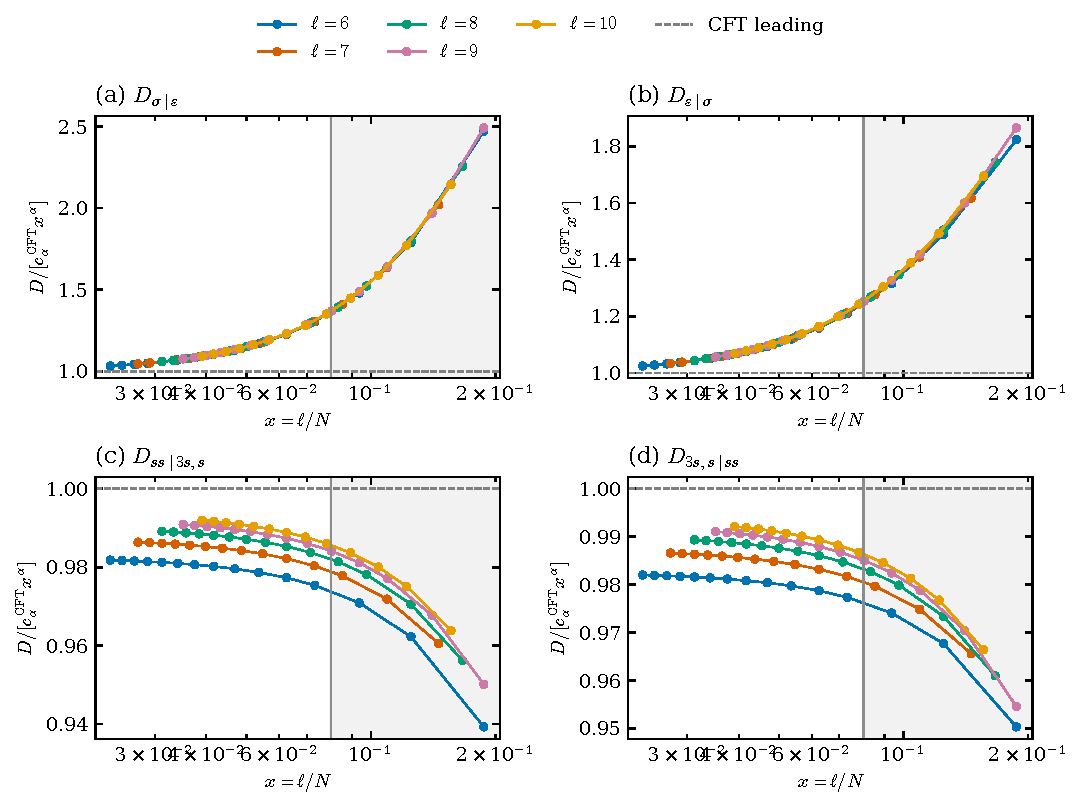
\includegraphics[width=.98\linewidth]{../figs/small_x_diagnostics.pdf}
\caption{Historical smaller-$x$ comparison, without fitting a lattice correction.
The ordinate is $R$ in Eq.~\eqref{eq:small-x-ratio}, with $\alpha=2$,
$c_2^{\rm CFT}=\pi^2/48$ in (a,b), and $c_2^{\rm CFT}=\pi^2/6$ in (c,d).
All data use $p=1/2$, natural logarithms, the 15 sizes through $N=256$
in Eq.~\eqref{eq:large-grid}, $\ell=6,\ldots,10$, and
$\ell/N\leq0.20$. Colors identify fixed $\ell$; line segments only connect
the computed sizes, not fitted curves. The horizontal dashed line is the
CFT leading prediction. Ising uses the critical periodic Hamiltonian
$H=-\sum XX-\sum Z$ and exact covariance matrices; the boson uses
charge codes $(1,1),(3,1)$, $q=2$, $z_j=e^{2\pi i j/N}$, $w_1=0$,
$W=10^8$, and the same normalized vertex/Jastrow states as the original
method. The small-$x$ ends of the curves compare intervals containing
different numbers of lattice sites; every panel contains 70 observations.
The vertical line marks $x_{\rm fit}=0.08$ and the shaded region contains
data excluded from fitting. The ratios themselves use no fitted parameters.}
\label{fig:small-x}
\end{figure}

\subsection{Step 8: extend the chain while retaining numerical precision}
\label{sec:extended-production}
\begin{equation}\mathcal D=\{2\operatorname{round}[30\,100^{j/48}]:j=0,\ldots,48\},\qquad \mathcal R=\{200+4j:j=0,\ldots,200\}.\label{eq:dense-grid}\end{equation}
\begin{align}
\mathcal N_{\rm ising}&=\mathcal N\cup\mathcal D\cup\mathcal R\cup\{4096+256j:j=0,\ldots,16\}\nonumber\\
&\quad\cup\{152,1024,1118,1146,1232,1356,1492,1528,1604,1644\}\nonumber\\
&\quad\cup\{1808,1852,1972,2048,2190,2354,2412,2654,2890,3000\}\nonumber\\
&\quad\cup\{3140,3216,3294,3436,3500,3552,3606,3660,3784,3854\}\nonumber\\
&\quad\cup\{3926,4000,4158,4222,4286,4426,4670,4734,4798,5000\}\nonumber\\
&\quad\cup\{5246,5310,5542,5758,6270,6526,6782,7038,7294,7550\}\nonumber\\
&\quad\cup\{7806,8000,8016,8032,8048,8064,8080,8096,8112,8128\}\nonumber\\
&\quad\cup\{8144\},\nonumber\\
\mathcal N_{\rm boson}&=\mathcal N\cup\mathcal D\cup\{100,104,168,292,322,354,428,472,512,762\}\nonumber\\
&\quad\cup\{924,1024,1118,1356,1492,1644,1808,2048,2412,2922\}\nonumber\\
&\quad\cup\{3540,3750,3916,4096,4234,4376,4608,4720,4834,5000\}\nonumber\\
&\quad\cup\{5222,5626,5810,6250,6466,6688,6918,7156,7402,7656\}\nonumber\\
&\quad\cup\{7920,8192,8436,8688,8948,9216,9462,9714,9974,10240\}\nonumber\\
&\quad\cup\{10488,10740,10998,11264,11764,12288,12800,13312,13814,14336\}\nonumber\\
&\quad\cup\{14840,15360,15864,16384\}.
\label{eq:extended-grid}\end{align}
All indices $j$ in these set definitions are integers within the stated bounds.

The earlier grid in Eq.~\eqref{eq:large-grid} remains a reference subset.
The active mixture fits use Eq.~\eqref{eq:extended-grid}; no intervals
longer than ten sites are added. The primary-to-primary sanity check
in Appendix~\ref{sec:primary-relative-entropy} retains its original
$N\leq256$ grid. The methods below change how the same finite-chain
states and entropies are evaluated, not their definitions.

\subsubsection{Fourier construction and local Ising transition solves}
At criticality the Majorana matrix is uniform apart from its boundary
twist, so its eigenmodes are known Fourier waves. Let $L=2N$ count
Majoranas, with indices $j=0,\ldots,L-1$, and set
$k_m=2\pi(m+t)/L$. The twist is $t=1/2$ for $I,\eps$ and $t=0$
for $\sigma$. Define $w_m=-\operatorname{sgn}(\sin k_m)$.
For the energy state reverse $w_m$ at $m=0,N-1,N,L-1$.
For the spin state set the two zero-mode weights $w_0,w_N$ to zero
and supply their parity explicitly. Then
\begin{equation}
 (\Gamma_a)_{ij}=\frac{i}{L}\sum_{m=0}^{L-1}w_m
 e^{ik_m(i-j)}+\begin{cases}
 [(-1)^i-(-1)^j]/L,&a=\sigma,\\0,&a=I,\eps.
 \end{cases}
 \label{eq:fourier-covariance}
\end{equation}
The imaginary notation in the Fourier sum yields a real antisymmetric
matrix. The last term is $vu^T-uv^T$, with $u_j=L^{-1/2}$ and
$v_j=(-1)^jL^{-1/2}$; it selects the same odd Ramond state as
Sec.~\ref{sec:large-ising}. This is an exact finite-chain construction,
using the free-fermion mode description of Refs.~\cite{Montes2017,PeschelEisler}.
Its energies are
\begin{equation}
 E_I=-2\csc\frac{\pi}{2N},\quad
 E_\sigma=-2\cot\frac{\pi}{2N},\quad
 E_\eps=E_I+8\sin\frac{\pi}{2N}.
 \label{eq:fourier-energies}
\end{equation}
A fast Fourier transform applies $\Gamma_a$ to a vector in
$O(N\log N)$ work. Thus the Hamiltonian eigensolve is unnecessary.

For the anchored transition in Sec.~\ref{sec:complement-ising}, let
$\Gamma'_b$ be the covariance after applying the local anchor.
Form $K=\id-\Gamma_a\Gamma'_b$ by applying the Fourier transform to
batches of columns. Factor the real matrix $K$ once with pivoted LU
(lower and upper triangular factors). Let $E_A$ be the first $2\ell$
columns of the identity. Solve only
\begin{equation}
 KZ=(\id-i\Gamma_a)E_A,\qquad
 \Gamma_{ab,A}=i\{E_A^T(\id-i\Gamma'_b)Z-\id_{2\ell}\}.
 \label{eq:local-transition-solve}
\end{equation}
The real and imaginary right-hand sides reuse the same LU factors.
The anchor overlap is $|\det K|^{1/4}/2^{N/2}$; its logarithm is
obtained from the LU diagonal. Reconstruct the local Gaussian operator
and restore the anchor, exactly as in the earlier Gram calculation.
We never construct a full complex transition covariance or its inverse.
The remaining dense factorization costs $O(N^3)$ arithmetic and the
stored real matrices cost $O(N^2)$ memory. The interval density matrices
still have dimension at most $2^{10}=1024$.

\subsubsection{Direct evaluation of small entropy remainders}
\label{sec:stable-entropy}
At very small fractions, subtracting $\log2-D^B$ or two almost equal
entropy traces loses relative precision. Instead, evaluate their
remainder directly with matrix-function divided differences
\cite{Higham}. The following identity is an algebraic numerical device,
not a CFT expansion or a new analytical entropy coefficient.

Set $f(t)=t\log t$, with $f(0)=0$. In a basis where a positive reference
matrix is $D=\operatorname{diag}(d_i)$, write
$H=D+E=V\operatorname{diag}(\lambda_k)V^\dagger$.
The first-order matrix derivative has diagonal $f'(d_i)E_{ii}$.
For the remainder diagonal, use
\begin{equation}
 \mathcal R_i=[f(H)-f(D)]_{ii}-f'(d_i)E_{ii}
 =\sum_k |(V^\dagger E)_{ki}|^2\,
 \frac{\lambda_k\log(\lambda_k/d_i)-\lambda_k+d_i}
      {(\lambda_k-d_i)^2}.
 \label{eq:stable-remainder}
\end{equation}
To verify it, expand $[f(H)]_{ii}=\sum_k|V_{ik}|^2f(\lambda_k)$,
use $\sum_k|V_{ik}|^2=1$ and
$E_{ii}=\sum_k|V_{ik}|^2(\lambda_k-d_i)$, and factor the scalar
Taylor remainder. Finally,
$(\lambda_k-d_i)V_{ik}=(EV)_{ik}$ converts its squared factor to
the numerator weight in Eq.~\eqref{eq:stable-remainder}.
At equal arguments the quotient is $1/(2d_i)$.
With $u=(\lambda-d)/d$, compute it as
\begin{equation}
 \frac1d\frac{(1+u)\log(1+u)-u}{u^2}
 =\frac1d\sum_{n=0}^{\infty}\frac{(-u)^n}{(n+1)(n+2)}.
 \label{eq:stable-scalar}
\end{equation}
The code uses ten terms only for $|u|<0.02$, where the omitted
tail is below double-precision accuracy, and the closed expression
otherwise. This series stabilizes a scalar matrix-function evaluation;
it is unrelated to a small-interval power-law fit.

For $D$ the eigenvalue matrix of the mixture on $A$ and $H$ the source
state in that basis, equal unit traces give
$S(\rho\|\mu)=\sum_i\mathcal R_i$. For the complement, first define
the local transition $T_{ab}^A=\Tr_B\ket a\bra b$.
The unweighted Gram matrix has blocks
$H=\left(\begin{smallmatrix}\rho_a^A&T_{ab}^A\\
(T_{ab}^A)^\dagger&\rho_b^A\end{smallmatrix}\right)$.
Its relation $H=2\mathcal G^*$ to the weighted Gram matrix is derived
in Sec.~\ref{sec:complement-gram}. Transform the two diagonal blocks
to their separate Schmidt eigenbases and let $D$ contain their
eigenvalues on its diagonal.
Then $E$ contains only the off-diagonal transition blocks, so its
first-order diagonal vanishes. If $P_a,P_b$ select the two state blocks,
the Gram entropy identity gives the deficit
$\delta_{a\mid b}\equiv\log2-D^B_{a\mid b}$ directly:
\begin{equation}
 \delta_{a\mid b}=\Tr P_a[f(H)-f(D)]
       =\sum_{i\in a}\mathcal R_i,\qquad
 \delta_{b\mid a}=\sum_{i\in b}\mathcal R_i.
 \label{eq:stable-deficit}
\end{equation}
Complex conjugating the entire Gram matrix preserves these real block
traces. Thus even a deficit much smaller than machine precision
relative to $\log2$ can be stored accurately on its own.

The identities are exact on a positive support. In double precision
we retain reference eigenvalues above $\tau=10^{-15}$ in each
symmetry sector. The discarded tails are a numerical approximation;
they are checked by varying $\tau$ to $10^{-14}$ and $10^{-16}$ at
every new size for $\ell=4,10$. We additionally compare with the original
trace-log and Gram formulas and with a high-precision, noncommuting
two-dimensional example. These checks, together with the larger-size
state-contraction tests, are reported in Appendix~\ref{sec:scaling-checks}.

\subsubsection{Boson scaling and the practical boundary}
The boson continues to use the exact sparse moment and small Pfaffian
reductions in Sec.~\ref{sec:boson-contraction} and
Appendix~\ref{sec:complement-pf-details}. The dense high-precision
minors depend on $\ell$, not on $N$. At the added sizes the moment
algebra uses 120 decimal digits before its final conversion to double
precision. Independent sampled entries use 160 digits and direct
pivoted Pfaffians instead of cached recursive minors.
Although the physical moment matrices are sparse, the current Python
pivot searches scan remaining indices. Their bookkeeping can cost
$O(N^2)$ time, in addition to the arithmetic and the $O(N\ell)$ stored
right-hand sides. This becomes the main practical obstacle before the
$2^\ell$ interval dimension changes. The measured limits and timings
below refer to this implementation on this machine; they are not
mathematical maximum chain lengths.
\begin{longtable}{lrrrr}
\caption{Measured largest completed chains, with three diagonal states, three transitions, both directions, and every $\ell=4,\ldots,10$. Wall time includes both interval calculations and endpoint cutoff checks. Memory is the process high-water resident set (GiB), not the size of one matrix; it may include allocations retained from preceding stages. The host has 32 GiB RAM. These are validated endpoints, not absolute mathematical limits.}
\label{tab:scaling-resources}\\\toprule
CFT & Largest $N$ & Seconds & Peak GiB & Minimum retained fraction\\\midrule
\endfirsthead
\toprule
CFT & Largest $N$ & Seconds & Peak GiB & Minimum retained fraction\\\midrule
\endhead
\bottomrule\endfoot
ising & 8192 & 93.46 & 9.0882 & $7.324\!\times\!10^{-4}$\\
boson & 16384 & 506.34 & 0.73204 & $3.662\!\times\!10^{-4}$\\
\end{longtable}
For Ising, doubling the largest tested $N$ would multiply the dominant stored matrix sizes by four, giving an estimated 36.4 GiB with the present allocation pattern, above this host\textquotesingle s RAM. The dense LU arithmetic would grow by about eight. For the boson, sparse index scans still permit further growth but become costly: doubling $N$ can quadruple that bookkeeping. Such extrapolations are estimates, not executed benchmarks. No larger size is claimed as validated.



\clearpage
\section{Small-interval fits and the leading-power test}
\label{sec:fits}
\subsection{Data selection and coefficient convention}
\label{sec:fit-selection}
The active mixture data use the grid in Eq.~\eqref{eq:extended-grid},
$\ell=6,\ldots,10$, and $p=1/2$. Let $x=\ell/N$ for the small
interval $A$, and $y=\ell/N$ for the small complement of the large
interval $B$. The common fitting windows are
\begin{align}
 W_x^{\rm Ising}&=(0,0.02],& W_x^{\rm boson}&=(0,0.1],\nonumber\\
 W_y^{\rm Ising}&=(0,0.002],& W_y^{\rm boson}&=(0,0.005].
 \label{eq:common-fit-windows}
\end{align}
Each window is shared by all six ordered pairs and by Free, $F_1$,
and $F_2$ for its CFT and interval type. Zero is an open lower bound;
there is no observation at zero. The two small-interval windows are
frozen. The large-boson upper cutoff is prescribed as $0.005$; the updated
coefficient and neighboring-cutoff checks are documented in
Appendix~\ref{sec:common-window-results}. In this revision,
the large-boson cutoff changes from $0.0047$ to $0.005$; the other
three windows are unchanged.
Every full fit and every omitted-size training set has at least forty
distinct $(N,\ell)$ observations. Exact counts and sampled endpoints
are in Appendix~\ref{sec:window-comparison}.
The overview figures show data through $x,y=0.20$ so the entire fitted
range is visible, with excluded data shaded. Per-pair figures in
Sec.~\ref{sec:window-selection} also provide fitting-window zooms.
Historical primary-to-primary comparisons on $N\leq256$ retain their
separately stated fitting window.
\begin{longtable}{llrrrrr}
\caption{Active mixture geometries, with all $\ell=6,\ldots,10$ at each listed size. The full grids are Eq.~\eqref{eq:extended-grid}. Counts are per direction. The four common fitting windows are Eq.~\eqref{eq:common-fit-windows}; all figures show fractions through $0.2$. Historical $\ell=11,12$ values remain archived and are excluded from this revision.}
\label{tab:scaling-grid}\\\toprule
Interval & CFT & $N_{\max}$ & Retained & Fit & Shown & Minimum fraction\\\midrule
\endfirsthead
\toprule
Interval & CFT & $N_{\max}$ & Retained & Fit & Shown & Minimum fraction\\\midrule
\endhead
\bottomrule\endfoot
small & ising & 8192 & 1650 & 1255 & 1645 & $7.324\!\times\!10^{-4}$\\
small & boson & 16384 & 630 & 598 & 625 & $3.662\!\times\!10^{-4}$\\
large & ising & 8192 & 1650 & 260 & 1645 & $7.324\!\times\!10^{-4}$\\
large & boson & 16384 & 630 & 317 & 625 & $3.662\!\times\!10^{-4}$\\
\end{longtable}

All coefficient tables report amplitudes of $x^r$ or $y^r$ itself.
Thus, if an archived file writes $\widetilde C(\pi x)^r$, its amplitude
in this report is $C=\pi^r\widetilde C$. For a free exponent the
conversion uses the \emph{fitted} exponent, whereas the theoretical
amplitude uses the theoretical exponent. Omitting this distinction
changes the coefficient error whenever those exponents differ.

\subsection{Free powers, one-term fits, and two-term fits}
The overview figures, the per-pair figures, and the principal tables
in Appendices~\ref{sec:allfits} and \ref{sec:complement-checks} all
use Eq.~\eqref{eq:common-fit-windows}. Consequently every comparison
of Free, $F_1$, and $F_2$ within a CFT and interval type uses the same
observations, including both directions of each primary pair.

To state the same procedure for both intervals, let $z$ denote $x$ for
the small interval or $y$ for its large complement. Let $q_i$ be the
observed $D^A_{a\mid b}$ or $\delta_{a\mid b}$, respectively, at $z_i$.
The theoretical leading power is $r_0=\alpha_{\rm CFT}$ in the first
case and $r_0=\beta_{\rm CFT}$ in the second; $r_1$ denotes the next
power listed in the corresponding theory table. We compare
\begin{align}
 F_{\rm free}(z)&=Cz^r,\qquad C>0,\quad r\ \hbox{free},\nonumber\\
 F_1(z)&=c_0z^{r_0},\qquad
 F_2(z)=c_0z^{r_0}+c_1z^{r_1}.
 \label{eq:fit}
\end{align}
The subscripts on $F_1,F_2$ count fitted coefficients. They have one
and two fitted parameters, respectively; the free-power fit also has
two. The exponent of $F_1$ is imposed, so its agreement cannot validate
that exponent independently. $F_2$ holds both powers fixed and fits
both coefficients without sign constraints. There is no constant term.
The CFT curve has no fitted parameters: it contains the supplied
$x^4,x^6$ terms for $I\leftrightarrow\eps$, the leading term for the
other small-interval pairs, and only the leading term for large intervals.

For every fitted model, use unweighted least squares in the observable:
\begin{equation}
 r_i=q_i-M(z_i),\qquad
 \widehat\theta=\underset{\theta}{\operatorname{argmin}}
       \sum_{i=1}^m r_i^2 .
 \label{eq:objective}
\end{equation}
Here $m$ is the retained sample count and $\theta$ the fitted parameters.
The symbol $r_i$ with a sample index denotes a residual, while $r$
without an index in Eq.~\eqref{eq:fit} is an exponent.
For the free fit we write $F=\exp(u)(z/z_\star)^r$, where $z_\star$
is the fitting cutoff; $C=\exp(u)z_\star^{-r}$. A logarithmic regression
of the data supplies only an initial guess. No theoretical exponent or
coefficient enters this optimization. An independent scalar search
profiles out the amplitude at each exponent and checks the predictions.
For $F_1,F_2$, a scaled design matrix
$X_{ij}=(z_i/z_\star)^{r_j}$ gives a linear least-squares solve;
its coefficients are divided by $z_\star^{r_j}$ before reporting.

\subsection{Residuals and validation measures}
For the theory amplitude $c_0^{\rm CFT}$, define
\begin{align}
 \mathrm{SSE}&=\sum_i r_i^2,&
 \mathrm{RMSE}&=\sqrt{\mathrm{SSE}/m},& R_i[\%]&=100r_i/q_i,\nonumber\\
 \mathrm{RMSrel}[\%]&=\sqrt{m^{-1}\sum_i R_i^2},&
 \mathrm{MAPE}[\%]&=m^{-1}\sum_i|R_i|,\nonumber\\
 \eta_c[\%]&=100(\widehat c_0/c_0^{\rm CFT}-1),&
 \eta_r[\%]&=100(\widehat r/r_0-1),\nonumber\\
 G[\%]&=100(1-\mathrm{RMSE}_M/\mathrm{RMSE}_{F_1}).
 \label{eq:metrics}
\end{align}
For the free fit, $\widehat c_0=C$. An imposed exponent has no measured
exponent deviation. Every residual ordinate is linear and shows ordinary
percentage tick values; only the horizontal interval fraction is logarithmic.
All reported indicators use the fitting window, even though figures
also show excluded data. A negative $G$ means a larger residual than $F_1$.
Because $F_1$ is nested in $F_2$, a smaller training residual for $F_2$
alone does not establish predictive improvement.

We therefore omit every point at one chain size, refit the remaining
sizes, and predict the omitted points. With $M^{(-N_i)}$ denoting that
refit, define
\begin{equation}
 \mathrm{CVRMSE}=\sqrt{m^{-1}\sum_i[q_i-M^{(-N_i)}(z_i)]^2},\qquad
 G_{\rm CV}[\%]=100(1-\mathrm{CVRMSE}_M/\mathrm{CVRMSE}_{F_1}).
 \label{eq:cv}
\end{equation}
The CSV retains every omitted-size fit, the maximum absolute residual,
parameter ranges across folds, and descriptive standard errors from
$[\mathrm{SSE}/(m-k)](J^TJ)^{-1}$, where $k$ is the parameter count
and $J$ is the prediction Jacobian. These deterministic data do not
support interpreting those errors as statistical confidence intervals.

\subsection{What the free-power test establishes}
An unweighted fit over a fixed window is most sensitive to its larger
observations. Adding tiny-$x$ points need not move its fitted exponent
to the asymptotic value. Appendix~\ref{sec:window-comparison} records
the retained fraction range and enforces the minimum sample count;
smaller trial windows with fewer than forty points are excluded.
The exponent is estimated without changing the objective or imposing
the predicted power. A stable exponent close
to CFT supports the leading-power prediction; a remaining amplitude
offset at fixed $\ell$ can still reflect finite lattice resolution.
Increasing $N$ alone does not take $\ell\to\infty$.
Ising full-window free-exponent deviations range from $-0.348\%$ to $+1.188\%$. $F_2$ improves size-holdout RMSE over $F_1$ in 6 of six directions. These statements use the prescribed fitting window and the sample-count requirements in Appendix~\ref{sec:window-comparison}.\par
Compact-boson full-window free-exponent deviations range from $-1.756\%$ to $-0.087\%$. $F_2$ improves size-holdout RMSE over $F_1$ in 4 of six directions. These statements use the prescribed fitting window and the sample-count requirements in Appendix~\ref{sec:window-comparison}.\par
The supplied next coefficients provide a separate test: the adopted common-window $x\leq0.02$ $F_2$ fits give $c_1=-170.71,-355.38$ for $I\mid\eps$ and $\eps\mid I$, respectively, whereas CFT gives $-8\pi^6/45$ and $-8\pi^6/21$. Their signed next-coefficient discrepancies are approximately $-0.122\%$ and $-2.966\%$. Table~\ref{tab:ising-small-parameters} gives all parameters from these same fits. Agreement of the leading exponent does not establish agreement of the next-order amplitude.\par
For the difficult Ising spin--energy pair, the window $x\leq0.001$ gives free exponents $1.999324,1.999296$, compared with two. The corresponding full amplitudes are $0.204756,0.204713$, compared with $\pi^2/48$. The order is $\sigma\mid\eps$, then $\eps\mid\sigma$. No analytical exponent is imposed in these fits.\par

The complete small-interval parameters and residual comparisons are in
Appendix~\ref{sec:allfits}. The plots below show every retained model;
curves outside the fitting window are extrapolations of a truncated
description. Nonpositive extrapolated values cannot be drawn on a
logarithmic entropy ordinate and are omitted from that curve only;
their signed residuals remain displayed.
\begin{figure}[p]\centering
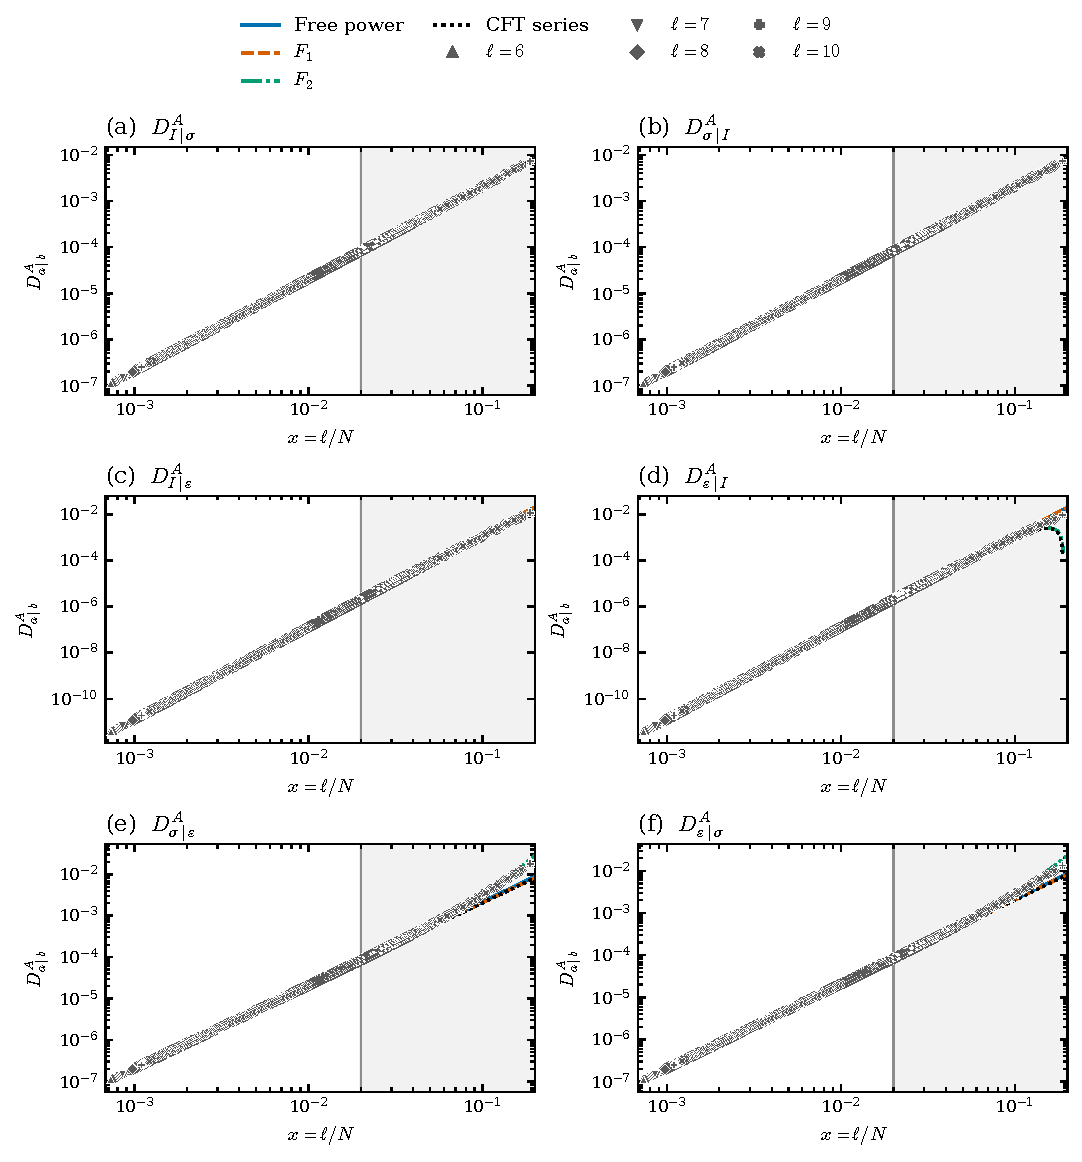
\includegraphics[width=.88\linewidth]{../figs/ising_small_value.pdf}
\caption{Both axes are logarithmic. Nonpositive values of an extrapolated truncated curve are omitted only from this logarithmic panel, while residual panels retain their predictions. Ising mixtures at $p=1/2$, $\ell=6,7,8,9,10$, and the chain-size set in Eq.~\eqref{eq:extended-grid}, with $32\leq N\leq8192$. There are 1645 displayed geometries per direction at $x\leq0.2$, of which 1255 satisfy $x\leq0.02$ and enter every fit. Marker shape identifies $\ell$; the vertical boundary and gray shading mark the fitting cutoff and excluded data. The periodic Ising Hamiltonian is $H=-\sum_jX_jX_{j+1}-\sum_jZ_j$; primaries use exact fermionic covariances, including the odd Ramond ground state for $\sigma$. Natural logarithms apply. Added sizes use the direct entropy remainder in Sec.~\ref{sec:stable-entropy}, with support cutoff $10^{-15}$. Blue solid is the free-power fit (two fitted parameters), orange dashed is $F_1$ (one), green dash--dot is $F_2$ (two), and black dotted is the supplied CFT series (zero). Powers and amplitudes use Eqs.~\eqref{eq:fit} and \eqref{eq:hierarchy}; all coefficients include powers of $\pi$. Fits minimize unweighted squared residuals in $D^A$. These curves use \texttt{scaling\_fit\_summary.csv}. The identical fits in Tables~\ref{tab:ising-small-parameters} and \ref{tab:ising-small-metrics} also have per-pair full-range and fitting-window views in Sec.~\ref{sec:pair-small_ising}.}
\label{fig:isingfits}
\end{figure}

\begin{figure}[p]\centering
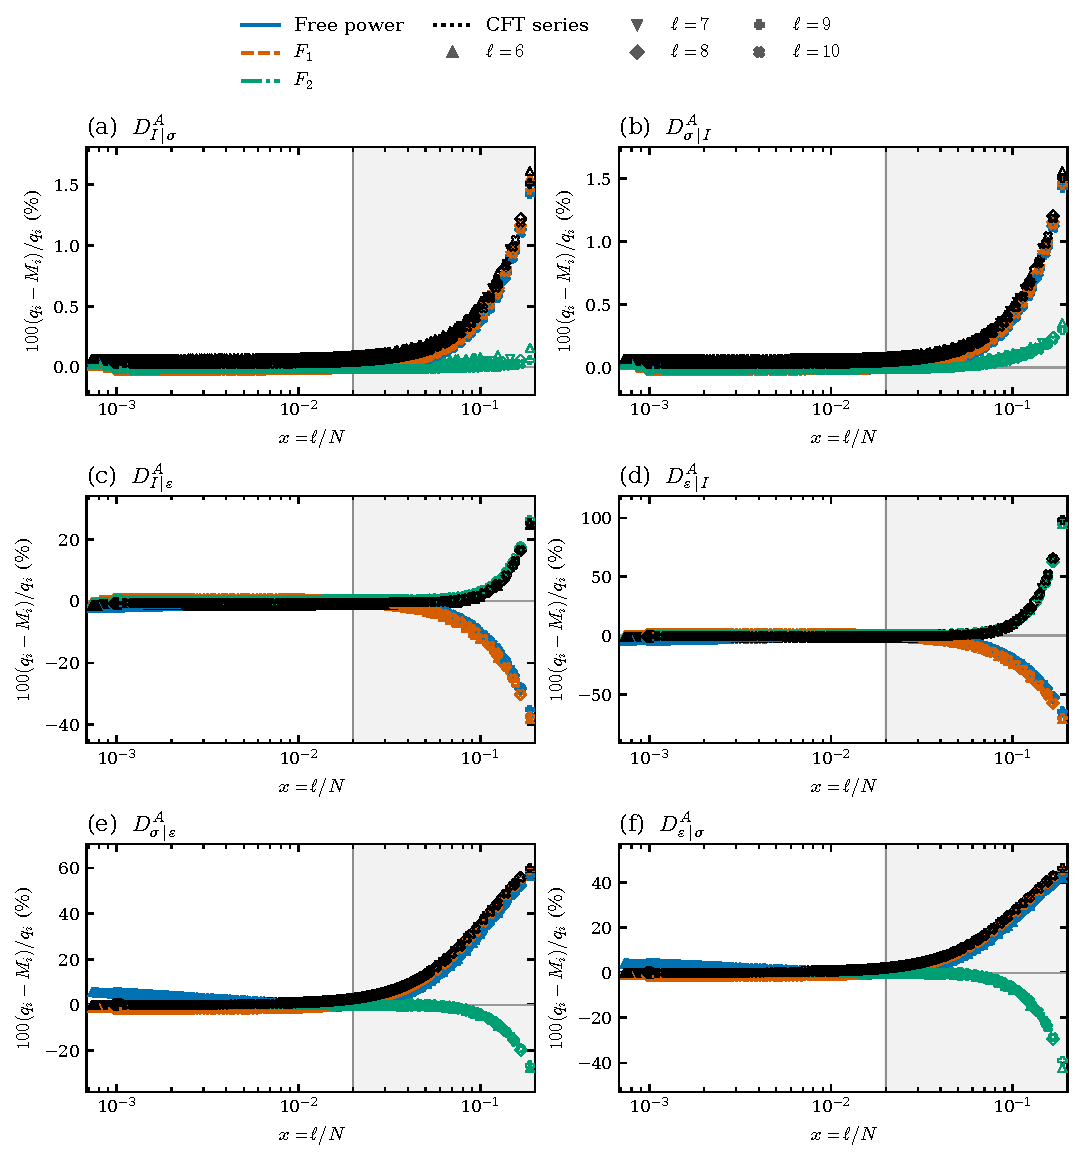
\includegraphics[width=.88\linewidth]{../figs/ising_small_residual.pdf}
\caption{The ordinate is $100(q_i-M_i)/q_i$ percent, with $q_i=D^A_i$ for a small interval and $q_i=\delta_i$ for a large interval; the horizontal zero line aids comparison. All four models have residual markers, colored as their curves. The residual ordinate is linear; the fraction axis is logarithmic. Ising mixtures at $p=1/2$, $\ell=6,7,8,9,10$, and the chain-size set in Eq.~\eqref{eq:extended-grid}, with $32\leq N\leq8192$. There are 1645 displayed geometries per direction at $x\leq0.2$, of which 1255 satisfy $x\leq0.02$ and enter every fit. Marker shape identifies $\ell$; the vertical boundary and gray shading mark the fitting cutoff and excluded data. The periodic Ising Hamiltonian is $H=-\sum_jX_jX_{j+1}-\sum_jZ_j$; primaries use exact fermionic covariances, including the odd Ramond ground state for $\sigma$. Natural logarithms apply. Added sizes use the direct entropy remainder in Sec.~\ref{sec:stable-entropy}, with support cutoff $10^{-15}$. Blue solid is the free-power fit (two fitted parameters), orange dashed is $F_1$ (one), green dash--dot is $F_2$ (two), and black dotted is the supplied CFT series (zero). Powers and amplitudes use Eqs.~\eqref{eq:fit} and \eqref{eq:hierarchy}; all coefficients include powers of $\pi$. Fits minimize unweighted squared residuals in $D^A$. These curves use \texttt{scaling\_fit\_summary.csv}. The identical fits in Tables~\ref{tab:ising-small-parameters} and \ref{tab:ising-small-metrics} also have per-pair full-range and fitting-window views in Sec.~\ref{sec:pair-small_ising}.}
\label{fig:isingresid}
\end{figure}

\begin{figure}[p]\centering
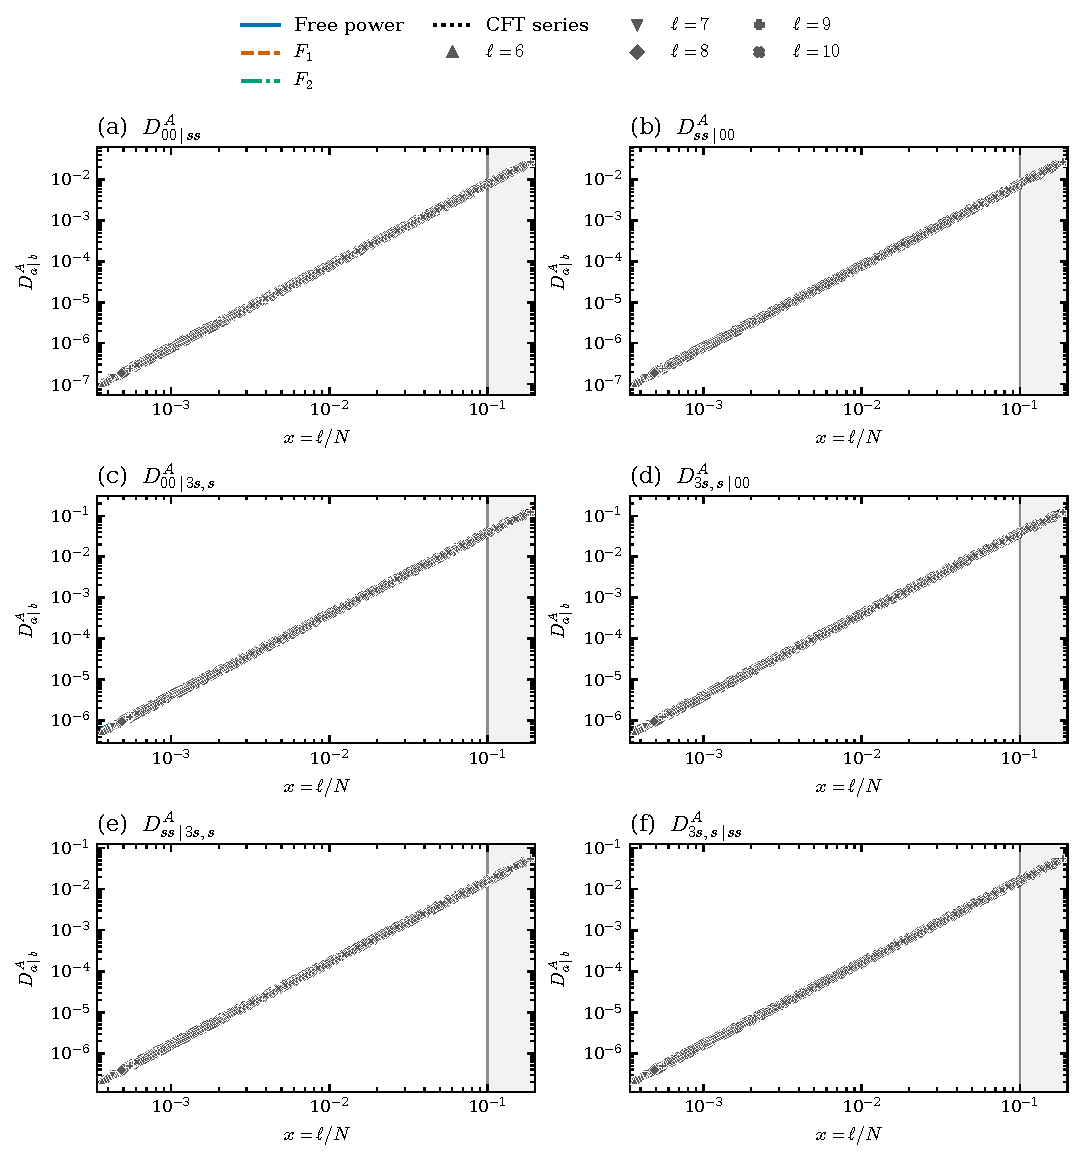
\includegraphics[width=.88\linewidth]{../figs/boson_small_value.pdf}
\caption{Both axes are logarithmic. Nonpositive values of an extrapolated truncated curve are omitted only from this logarithmic panel, while residual panels retain their predictions. Compact-boson mixtures at $p=1/2$, $\ell=6,7,8,9,10$, and the chain-size set in Eq.~\eqref{eq:extended-grid}, with $32\leq N\leq16384$. There are 625 displayed geometries per direction at $x\leq0.2$, of which 598 satisfy $x\leq0.1$ and enter every fit. Marker shape identifies $\ell$; the vertical boundary and gray shading mark the fitting cutoff and excluded data. The boson uses $s=1/\sqrt2$, $q=2$, charge codes $(0,0),(1,1),(3,1)$, $z_j=e^{2\pi i j/N}$, $w_1=0$, and $W=10^8$; moment algebra uses 100 digits through $N=256$ and 120 digits at the added sizes. Natural logarithms apply. Added sizes use the direct entropy remainder in Sec.~\ref{sec:stable-entropy}, with support cutoff $10^{-15}$. Blue solid is the free-power fit (two fitted parameters), orange dashed is $F_1$ (one), green dash--dot is $F_2$ (two), and black dotted is the supplied CFT series (zero). Powers and amplitudes use Eqs.~\eqref{eq:fit} and \eqref{eq:hierarchy}; all coefficients include powers of $\pi$. Fits minimize unweighted squared residuals in $D^A$. These curves use \texttt{scaling\_fit\_summary.csv}. The identical fits in Tables~\ref{tab:boson-small-parameters} and \ref{tab:boson-small-metrics} also have per-pair full-range and fitting-window views in Sec.~\ref{sec:pair-small_boson}.}
\label{fig:bosonfits}
\end{figure}

\begin{figure}[p]\centering
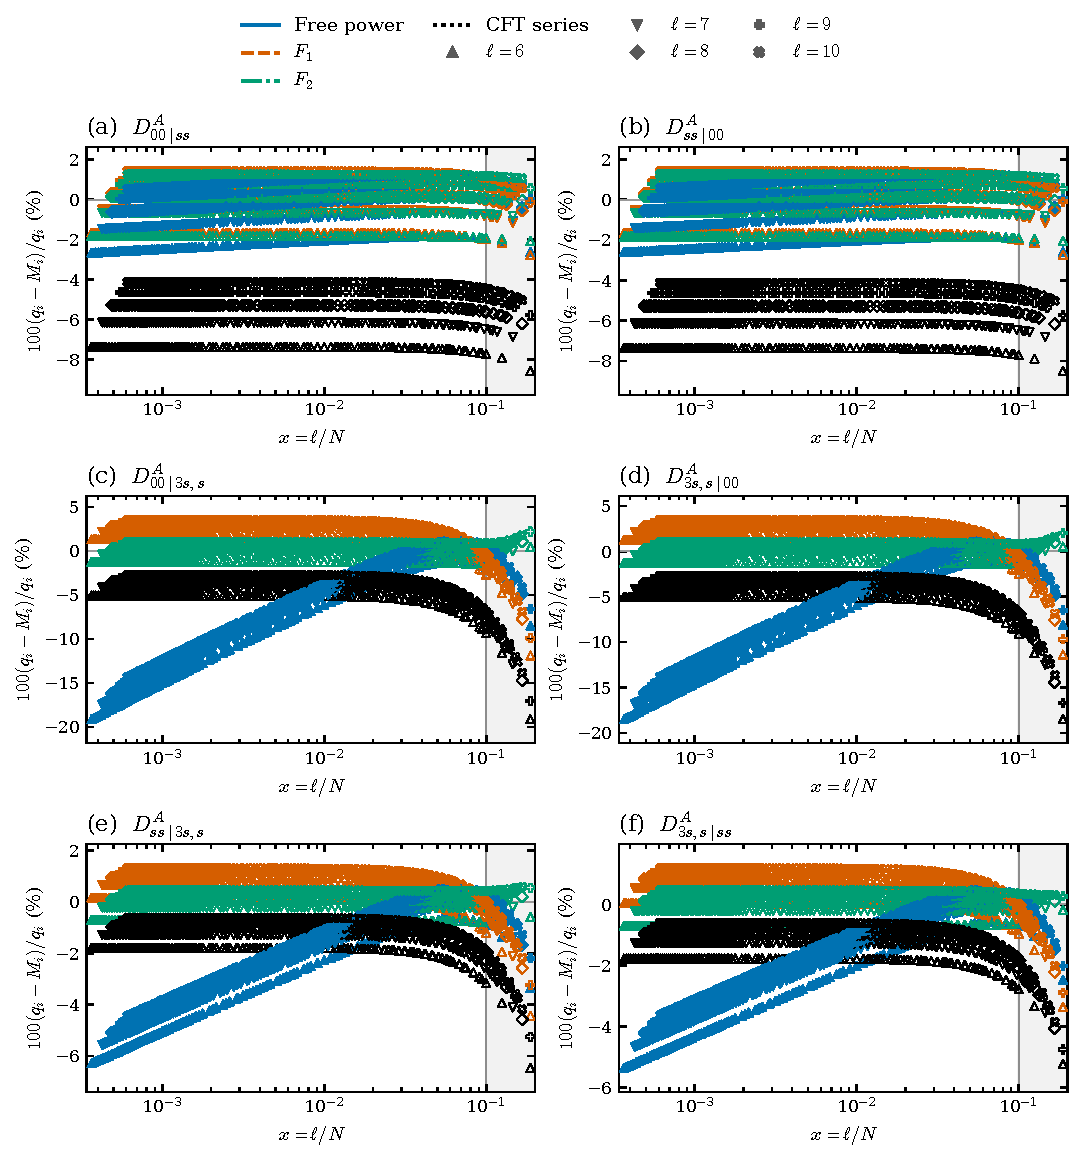
\includegraphics[width=.88\linewidth]{../figs/boson_small_residual.pdf}
\caption{The ordinate is $100(q_i-M_i)/q_i$ percent, with $q_i=D^A_i$ for a small interval and $q_i=\delta_i$ for a large interval; the horizontal zero line aids comparison. All four models have residual markers, colored as their curves. The residual ordinate is linear; the fraction axis is logarithmic. Compact-boson mixtures at $p=1/2$, $\ell=6,7,8,9,10$, and the chain-size set in Eq.~\eqref{eq:extended-grid}, with $32\leq N\leq16384$. There are 625 displayed geometries per direction at $x\leq0.2$, of which 598 satisfy $x\leq0.1$ and enter every fit. Marker shape identifies $\ell$; the vertical boundary and gray shading mark the fitting cutoff and excluded data. The boson uses $s=1/\sqrt2$, $q=2$, charge codes $(0,0),(1,1),(3,1)$, $z_j=e^{2\pi i j/N}$, $w_1=0$, and $W=10^8$; moment algebra uses 100 digits through $N=256$ and 120 digits at the added sizes. Natural logarithms apply. Added sizes use the direct entropy remainder in Sec.~\ref{sec:stable-entropy}, with support cutoff $10^{-15}$. Blue solid is the free-power fit (two fitted parameters), orange dashed is $F_1$ (one), green dash--dot is $F_2$ (two), and black dotted is the supplied CFT series (zero). Powers and amplitudes use Eqs.~\eqref{eq:fit} and \eqref{eq:hierarchy}; all coefficients include powers of $\pi$. Fits minimize unweighted squared residuals in $D^A$. These curves use \texttt{scaling\_fit\_summary.csv}. The identical fits in Tables~\ref{tab:boson-small-parameters} and \ref{tab:boson-small-metrics} also have per-pair full-range and fitting-window views in Sec.~\ref{sec:pair-small_boson}.}
\label{fig:bosonresid}
\end{figure}


\clearpage
\section{Large complementary intervals}
\label{sec:complement}

Throughout this report, $\alpha$ denotes the leading small-interval
power and $\beta$ the leading large-interval deficit power.
For the latter, $\beta_{\rm CFT}$ is the analytical prediction and
$\widehat\beta$ is the freely fitted exponent.

\subsection{Step 1: specify the interval and the observable}
The primaries and their lattice representatives are the same as in
Secs.~\ref{sec:construction} and \ref{sec:large-scales}.
Let $A=\{0,\ldots,\ell-1\}$ contain $\ell$ consecutive sites, and let
$B=\{\ell,\ldots,N-1\}$ be its complement on the periodic chain.
Define
\begin{equation}
 y=\frac{\ell}{N},\qquad x_B=1-y,\qquad
 \rho_a^B=\Tr_A\ket a\bra a,\qquad
 \bar\rho_{ab}^B=\frac{\rho_a^B+\rho_b^B}{2}.
 \label{eq:complement-geometry}
\end{equation}
Here $a,b$ label distinct primaries, $p=1/2$ is the mixing probability,
and $y$ always denotes the small complement fraction in this section.
The theory manuscript uses $y$ for a mixing probability in some formulas;
that manuscript variable is set to $1/2$ here. Its small parameter
$\epsilon=1-x$ is our $y$.
For each ordered pair we calculate
\begin{equation}
 D^B_{a\mid b}=\Tr\rho_a^B(\log\rho_a^B-\log\bar\rho_{ab}^B),
 \qquad \delta_{a\mid b}(y)=\log2-D^B_{a\mid b}.
 \label{eq:complement-deficit}
\end{equation}
All logarithms are natural. The two directions use the same incoherent
mixture; the source state changes. Positivity and
$\bar\rho_{ab}^B\geq\rho_a^B/2$ imply $0\leq D^B_{a\mid b}\leq\log2$.
The manuscript predicts $D^B_{a\mid b}\to\log2$ as $y\to0$.
The deficit resolves the approach to this limit more clearly than
$D^B_{a\mid b}$ alone.

The active mixture grid is Eq.~\eqref{eq:extended-grid}, with
$\ell=6,\ldots,10$. All models and all six directions use
$0<y\leq0.002$ for Ising or $0<y\leq0.005$ for the boson,
as in Eq.~\eqref{eq:common-fit-windows}. The boson window is prescribed;
its coefficient comparisons are in Appendix~\ref{sec:common-window-results}.
On the adopted large-interval windows, $F_2$ improves the leading coefficient over $F_1$ in 6 of six Ising directions and 4 of six compact-boson directions. Omitted-size prediction improves in 6 of six Ising directions and 2 of six compact-boson directions. The boson uses $0<y\leq0.005$; Appendix~\ref{sec:common-window-results} gives the full comparison.

The displayed range is $y\leq0.20$, or $x_B\geq0.80$.
Fits use $x_B\geq0.998$ for Ising and $x_B\geq0.995$ for the
boson. Counts are in Table~\ref{tab:scaling-grid}. Previously computed
$\ell=4,5,11,12$ observations remain archived and are excluded.
The overview figures and summary tables use the same fits as the
per-pair views in Sec.~\ref{sec:window-selection}.

\subsection{Step 2: replace the large matrix by a Gram matrix}
\label{sec:complement-gram}
Although $\rho_a^B$ acts on $2^{N-\ell}$ basis states, a pure global
state has Schmidt rank at most $2^\ell$ across this cut. A mixture of
two such states has rank at most $2^{\ell+1}$. To use this fact we need
both the individual matrices on $A$ and the transition matrix
\begin{equation}
 \rho_a^A=\Tr_B\ket a\bra a,\qquad
 T_{ab}^A=\Tr_B\ket a\bra b .
 \label{eq:complement-transition}
\end{equation}
The transition is generally neither Hermitian nor a density matrix.
It records how the two Schmidt supports overlap on $B$; the individual
$\rho_a^A,\rho_b^A$ do not determine that overlap.

For the derivation only, write
$\ket a=\sum_{u,v}X_a(v,u)\ket u_A\ket v_B$,
where $u$ and $v$ enumerate spin configurations.
Let $Z=(X_a,X_b)/\sqrt2$. Then
$ZZ^\dagger=\bar\rho_{ab}^B$, while its small Gram matrix is
\begin{equation}
 {\cal G}=Z^\dagger Z
 =\frac12\begin{pmatrix}
  (\rho_a^A)^T &(T_{ab}^A)^*\\
  (T_{ab}^A)^T&(\rho_b^A)^T
 \end{pmatrix}.
 \label{eq:complement-gram}
\end{equation}
The transpose and complex conjugation follow from assigning the $A$
configuration to the column of $X_a$; they must not be dropped.
The nonzero eigenvalues $\lambda_k$ of $\mathcal G$ are exactly those
of $\bar\rho_{ab}^B$. If $v_k$ is its normalized eigenvector, define
$P_a=\operatorname{diag}(\id_{2^\ell},0)$ and
$P_b=\operatorname{diag}(0,\id_{2^\ell})$.
The corresponding normalized large-space vector is
$w_k=Zv_k/\sqrt{\lambda_k}$.
Using $X_a=\sqrt2 ZE_a$, where $E_a$ embeds the first block, gives
$\bra{w_k}\rho_a^B\ket{w_k}=2\lambda_k v_k^\dagger P_a v_k$.
Purity equates the nonzero spectra of $\rho_a^A$ and $\rho_a^B$.
Therefore the complete entropy is
\begin{equation}
 D^B_{a\mid b}
 =\Tr(\rho_a^A\log\rho_a^A)
   -2\sum_{\lambda_k>0}\lambda_k
       (v_k^\dagger P_a v_k)\log\lambda_k .
 \label{eq:complement-entropy}
\end{equation}
Replace $P_a$ by $P_b$ and $\rho_a^A$ by $\rho_b^A$ for the other
direction. This form avoids division by small eigenvalues.
Multiplying $T_{ab}^A$ by one constant phase only conjugates
$\mathcal G$ by a block-diagonal unitary and leaves both entropies unchanged.

We diagonalize common quantum-number blocks on $B$. An Ising block
has parity $\mathfrak p_a(-1)^{|u|}$, with
$\mathfrak p_I=\mathfrak p_\varepsilon=1$,
$\mathfrak p_\sigma=-1$, and $|u|$ the number of occupied sites in $u$.
The scalar parity $\mathfrak p_a$ is distinct from the block projector $P_a$.
A boson block has $M_a-|u|$ occupied sites on $B$, where
$M_a$ is the total occupation in state $a$.
At $\ell=12$ the full Gram dimension is 8192; the largest symmetry
blocks are 4096 for Ising and 1716 for the boson pairs. We construct
each common-$B$ block directly, avoiding the full Gram allocation.
The production calculation constructs no state or matrix of dimension $2^{N-\ell}$.

For the new $\ell=11,12$ data, an additional numerical reduction
retains the occupied Schmidt vectors. In each local symmetry sector,
diagonalize $\rho_a^A$ and collect eigenvectors with eigenvalues
$\mu_{a,j}>\tau_s=10^{-16}$ in $U_a$; let
$\Lambda_a=\operatorname{diag}(\mu_{a,j})$ contain the retained values.
Use $U_b,\Lambda_b$ for the other state. Here these matrices collect
the retained vectors and values from all local sectors; the calculation
still diagonalizes each common-$B$ sector separately. With
$V=\operatorname{diag}(U_a^*,U_b^*)$, the projected Gram is
\begin{equation}
 {\cal G}_s=V^\dagger{\cal G}V
 =\frac12\begin{pmatrix}
 \Lambda_a &(U_a^\dagger T_{ab}^A U_b)^*\\
 (U_a^\dagger T_{ab}^A U_b)^T&\Lambda_b
 \end{pmatrix}.
 \label{eq:complement-support}
\end{equation}
Use the same source-weight formula in Eq.~\eqref{eq:complement-entropy},
with projectors onto the two retained blocks. The diagonal
$\Tr\rho_a^A\log\rho_a^A$ is evaluated from the corresponding
eigenvalues with the original entropy threshold $10^{-15}$.
This discards small Schmidt weights and is a numerical approximation.
We record $|1-\Tr\Lambda_a|$ and check the entropies against the full
Gram calculation and against $\tau_s=10^{-17},10^{-15}$ in
Sec.~\ref{sec:complement-extension-checks}. The $N=256$ benchmark
data themselves use the full Gram matrices.

\subsection{Step 3: obtain Ising transitions from anchored Gaussian states}
\label{sec:complement-ising}
Use the exact parity-resolved covariance $G_a$ of
Sec.~\ref{sec:large-ising} for each of $I,\sigma,\varepsilon$.
In our convention $\langle\gamma_r\gamma_s\rangle
=\delta_{rs}-i(G_a)_{rs}$ and $G_a^2=-\id$.
The $\gamma_r$ are Jordan--Wigner Majorana operators, with site zero
first. Distinct primaries are orthogonal, so a transition formula that
divides by $\langle b|a\rangle$ is singular. We remove that singularity
by acting on the bra state with a local Hermitian unitary:
\begin{equation}
 U_A=\begin{cases}
  \gamma_0=X_0,&\text{pairs containing }\sigma,\\
  i\gamma_0\gamma_1=-Z_0,& I,\varepsilon\text{ pair},
 \end{cases}
 \qquad \ket{b'}=U_A\ket b .
 \label{eq:complement-anchor}
\end{equation}
Here $X_0,Z_0$ are Pauli matrices on site zero.
The first choice changes parity; the second couples the two even
states. Both give a nonzero overlap with $\ket a$ on the tested grid.
They are computational devices and do not change the production
primary states.

Conjugation gives $G_{b'}=R G_bR^T$, where $R$ is diagonal with minus
signs at index $0$ for the first case or at $0,1$ for the second case,
and plus signs elsewhere. In the first case the true Majorana
reflection differs by an overall minus sign, which cancels in the covariance.
The Gaussian overlap and product rules
\cite{Bravyi,Surace} give, in our convention,
\begin{align}
 K&=\id-G_aG_{b'},&
 o&=|\langle b'|a\rangle|
   =2^{-N/2}\det(K)^{1/4},\nonumber\\
 Q&=(\id-iG_{b'})K^{-1}(\id-iG_a),&
 G_*&=i(Q-\id).
 \label{eq:complement-transition-covariance}
\end{align}
The inverse denotes a linear solve. We evaluate
$\log o=\tfrac14\sum_j\log s_j(K)-\tfrac N2\log2$
from the positive singular values $s_j(K)$, avoiding a large determinant.
The matrix $G_*$ is complex antisymmetric and describes the trace-one
operator $\ket a\bra{b'}/\langle b'|a\rangle$.
It need not describe a physical density matrix.

Restrict $G_*$ to its first $2\ell$ Majoranas. For any complex
antisymmetric matrix $H$ on those modes define the operator
\begin{equation}
 {\cal R}(H)=2^{-\ell}
   \sum_{\substack{S\subset\{0,\ldots,2\ell-1\}\\ |S|\ {\rm even}}}
   i^{|S|/2}\operatorname{Pf}(H_S)
   \prod_{r\in S}^{\longrightarrow}\gamma_r ,
 \qquad \operatorname{Pf}(H_\varnothing)=1 .
 \label{eq:complement-wick}
\end{equation}
$H_S$ is the principal submatrix on $S$, the product is in increasing
index order, and $\operatorname{Pf}$ denotes the Pfaffian introduced in
Sec.~\ref{sec:boson-contraction}. This is Wick's theorem expressed in
the Majorana operator basis. Undoing the local anchor gives
\begin{equation}
 T_{ab}^A=o\,{\cal R}((G_*)_A)U_A
 \quad\text{up to one overall phase}.
 \label{eq:complement-ising-transition}
\end{equation}
The code evaluates all principal Pfaffians recursively and converts
the Pauli-string coefficients to matrix entries with a Walsh transform.
It requires $O(\ell^2 4^\ell)$ local work and a $2N$-dimensional
covariance solve, without a full-chain wavefunction.
For the added diagonal matrices at $\ell=12$, the same reconstruction
gives $\rho_a^A={\cal R}((G_a)_A)$. It avoids forming and rotating
all 24 dense Majorana matrices; its reduction to $\ell=10$ is checked
against the existing Schur-based diagonal matrices.
The anchor and this reconstruction are project adaptations of the
published Gaussian identities. Their explicit-wavefunction checks are
reported in Sec.~\ref{sec:complement-checks}.

\subsection{Step 4: contract different boson occupation sectors exactly}
\label{sec:complement-boson}
The same conformal-block/Jastrow amplitudes of
Eq.~\eqref{eq:pf-amplitude} are used, with endpoint $W=10^8$.
To distinguish charge labels from state names, denote ket charges by
$(a_1,b_1)$ and bra charges by $(a_2,b_2)$, with
$(0,0),(1,1),(3,1)$ representing $00,ss,3s,s$.
Their occupied-site counts are $M_i=(N-a_i-b_i)/2$.
Let $U,V\subset A$ be the occupied sites in the ket and bra configurations;
$Y\subset B$ is their common occupied environment. A transition element
can be nonzero only when
\begin{equation}
 m=M_1-|U|=M_2-|V|,\qquad 0\leq m\leq N-\ell .
 \label{eq:complement-charge-selection}
\end{equation}
Thus different occupation numbers of the global primaries are fully
compatible with a nonzero transition on $A$.

Set $z_j=e^{2\pi i j/N}$, $g_i(z)=(1-z/W)^{b_i}$,
and define the unnormalized local polynomial
\begin{equation}
 L_i(U)=\prod_{j\in U}z_j^{a_i+1}g_i(z_j)
        \prod_{\substack{j<k\\j,k\in U}}(z_j-z_k)^2 .
 \label{eq:complement-local-boson}
\end{equation}
Splitting the full occupied set into $U\cup Y$ in the ket and
$V\cup Y$ in the bra, and using
$\overline{z_i-z_j}=-(z_i-z_j)/(z_i z_j)$, yields
\begin{align}
 (T_{12}^A)_{UV}
 &=\frac{L_1(U)\overline{L_2(V)}}{\sqrt{{\cal Z}_1{\cal Z}_2}}
       \prod_{j\in V}z_j^{-2m}\ {\cal E}_{UV},\nonumber\\
 {\cal E}_{UV}
 &=\sum_{\substack{Y\subset B\\|Y|=m}}
   \prod_{\substack{i<j\\i,j\in Y}}(z_i-z_j)^4
   \prod_{i\in Y}\left[
       w(z_i)\prod_{j\in A}(z_j-z_i)^{2\nu_j}\right],\nonumber\\
 \nu_j&=\mathbf1_{j\in U}+\mathbf1_{j\in V},\nonumber\\
 w(z)&=z^\kappa g_1(z)\overline{g_2(z)},\qquad
 \kappa=a_1-a_2-2M_2+2 .
 \label{eq:complement-environment}
\end{align}
Here $\mathcal Z_i$ is the full norm sum of state $i$.
The key identity is $2m+\sum_j\nu_j=M_1+M_2=:d$:
the moment-matrix dimension $d$ is independent of $U,V$.

To evaluate the environment sum, introduce the column
$f(z)=(1,z,\ldots,z^{d-1})^T$ and its derivative $f'(z)$.
The skew moment matrix on the environment is
\begin{equation}
 D_B=\sum_{j\in B}w(z_j)
       [f(z_j)f'(z_j)^T-f'(z_j)f(z_j)^T].
 \label{eq:complement-cross-moment}
\end{equation}
At each site $j\in A$, include no column if $\nu_j=0$,
$f(z_j)$ if $\nu_j=1$, and the two columns $f(z_j),f'(z_j)$
if $\nu_j=2$. Put these columns, in site order, in $E_{UV}$.
With $q=\sum_j\nu_j$ and
$\Delta_{\rm ext}=\prod_{i<j\in A}(z_j-z_i)^{\nu_i\nu_j}$,
the discrete confluent-Vandermonde identity gives
\begin{equation}
 {\cal E}_{UV}=
 \frac{(-1)^{q(q-1)/2}}{\Delta_{\rm ext}}\,
 \operatorname{Pf}
 \begin{pmatrix}D_B&E_{UV}\\-E_{UV}^T&0\end{pmatrix}.
 \label{eq:complement-bordered-pf}
\end{equation}
This follows by expanding the moment Pfaffian over distinct environment
sites. The confluent determinant contains their fourth-power Vandermonde,
the external factor $\Delta_{\rm ext}$, and the cross factors in
Eq.~\eqref{eq:complement-environment}. It extends the norm-sum construction
of St\'ephan and Pollmann \cite{Stephan} to a bra and ket with different
charges. It is an exact contraction of the interacting spin wavefunction.

Computing a new $d$-dimensional Pfaffian for every $U,V$ would waste
work. We instead use full-circle root-of-unity moments, remove the
$\ell$ sites of $A$ by a rank-$2\ell$ update, and cache the resulting
small Pfaffian minors. Odd $d$ and singular even cross moments require
the exact border/regularizer construction in
Sec.~\ref{sec:complement-pf-details}. All large-$N$ moment work then
uses sparse matrices; the final minors have at most $2\ell+1$ indices.
Through $N=256$ we evaluate the cancellation-prone moment algebra at 100 decimal digits
before converting $T_{12}^A$ to double precision.

\subsection{Step 5: test leading and next powers from CFT}
\label{sec:complement-theory}
The analytical source is \texttt{manuscript\_theory/main3.tex}
\cite{theoryLarge}. Its compiled \texttt{main.pdf} is an older version
without the worked examples used here. In the mixing operator product
expansion, let $\Delta$ be the lowest exchanged scaling dimension and
$c_{ab}$ its normalized coefficient. At $p=1/2$ the leading deficit is
\begin{equation}
 \delta_{a\mid b}(y)=B_{ab}y^{\beta_{\rm CFT}}+\cdots,\qquad
 \beta_{\rm CFT}=2\Delta,\qquad
 B_{ab}=\pi^{2\Delta}|c_{ab}|^2
 \frac{\sqrt\pi\,\Gamma(1+\Delta)}{4\Gamma(3/2+\Delta)}.
 \label{eq:complement-leading}
\end{equation}
$\Gamma$ is Euler's gamma function. In particular, $B_{ab}$ includes
$\pi^{\beta_{\rm CFT}}$. Each leading coefficient is shared by the
two directions; their higher-order coefficients need not coincide.
\begin{table}[htbp]\centering\small
\begin{tabular}{llccc}\toprule
CFT & Pair (both directions) & $\beta_{\rm CFT}$ & $B_{ab}$ & Next power\\\midrule
Ising & $I,\sigma$ & $1/4$ & $\pi^{3/4}\Gamma(9/8)/[4\Gamma(13/8)]$ & $1/2$\\
Ising & $I,\eps$ & $2$ & $\pi^2/3$ & $4$\\
Ising & $\sigma,\eps$ & $1/4$ & $\pi^{3/4}\Gamma(9/8)/[16\Gamma(13/8)]$ & $1/2$\\
Boson & $00,ss$ & $1$ & $\pi^2/8$ & $2$\\
Boson & $00,3s,s$ & $5$ & $5\pi^6/64$ & $6$\\
Boson & $ss,3s,s$ & $2$ & $\pi^2/3$ & $3$ (allowed)\\\bottomrule
\end{tabular}
\caption{Leading large-interval amplitudes multiplying $y^\beta$ and
next powers used in $F_2$, at $p=1/2$ and $s=1/\sqrt2$.
The Ising spin--energy channel includes $|c_{\sigma\eps}|^2=1/4$.
For boson charge codes $(a_i,b_i)$,
$\Delta=[(a_1-a_2)^2+(b_1-b_2)^2]/4$ and $|c_{ab}|=1$.
The last next power follows from the manuscript's general three-point
sector rather than a separately evaluated example; its coefficient may
vanish. No next-order coefficient is supplied or derived here.}
\label{tab:complement-theory}
\end{table}

The manuscript's Ising examples explicitly identify four-spin terms
of order $y^{1/2}$ and later two-spin--energy terms of order $y^{5/4}$;
the first correction retained in $F_2$ is $y^{1/2}$. The identity--energy
example specifies a remainder of order $y^4$. The boson vacuum examples
specify orders $y^2$ and $y^6$. For the remaining boson pair, the general
subsection ``Three point function'' contains powers
$2\Delta_{L'}+\Delta_L$: the exchanged vertex has $\Delta_{L'}=1$
and a current has $\Delta_L=1$, giving the candidate power three.
This identifies an allowed sector, not a proved nonzero total
coefficient after replica continuation. We consequently interpret
that pair's $F_2$ as a test of the next allowed power. This qualification
also prevents an $O(y^r)$ remainder from being mistaken for a known
coefficient. No universal increment of two is imposed for large intervals.

\begin{equation}
 F_{\rm free}(y)=Cy^{\widehat\beta},\qquad
 F_1(y)=c_0y^{\beta_{\rm CFT}},\qquad
 F_2(y)=c_0y^{\beta_{\rm CFT}}+c_1y^{\beta_1}.
 \label{eq:complement-fit}
\end{equation}
Here $\beta_1$ is the next power in Table~\ref{tab:complement-theory}.
Only the exponents of $F_1,F_2$ are imposed; all their coefficients
are fitted separately in each direction. ``CFT leading'' always means
$B_{ab}y^{\beta_{\rm CFT}}$, with neither parameter fitted.
For completeness, the one-term solution is
\begin{equation}
 c_0=\frac{\sum_i y_i^{\beta_{\rm CFT}}\delta_i}
                 {\sum_i y_i^{2\beta_{\rm CFT}}}.
 \label{eq:complement-fixed-fit}
\end{equation}
The fits use the CFT-wide windows in Eq.~\eqref{eq:common-fit-windows}:
$y\leq0.002$ for Ising and $y\leq0.005$ for the boson. Every
direction uses the same window as its reverse. Figures show data
through $y\leq0.20$, with fitting-window zooms in the per-pair views.
The objective, coefficient convention, residuals and size cross-validation
are exactly Eqs.~\eqref{eq:objective}, \eqref{eq:metrics} and \eqref{eq:cv}.
\begin{equation}
 R_i=100[\delta_i-M(y_i)]/\delta_i,\qquad
 \eta_\beta=100(\widehat\beta/\beta_{\rm CFT}-1).
 \label{eq:complement-fit-metrics}
\end{equation}
\begin{equation}
 \mathrm{CVRMSE}=\sqrt{m^{-1}\sum_i[\delta_i-M^{(-N_i)}(y_i)]^2}.
 \label{eq:complement-cv}
\end{equation}
The residual sign in the entropy $D^B=\log2-\delta$ is opposite to
the deficit residual. Tables in Appendix~\ref{sec:complement-checks}
separate Free, $F_1$, $F_2$ and CFT rows for all twelve directions.
\subsection{Results}
\label{sec:complement-results}
Ising full-window free-exponent deviations range from $-0.074\%$ to $+5.861\%$. $F_2$ improves size-holdout RMSE over $F_1$ in 6 of six directions. These statements use the prescribed fitting window and the sample-count requirements in Appendix~\ref{sec:window-comparison}.\par
Compact-boson full-window free-exponent deviations range from $-0.438\%$ to $-0.074\%$. $F_2$ improves size-holdout RMSE over $F_1$ in 2 of six directions. These statements use the prescribed fitting window and the sample-count requirements in Appendix~\ref{sec:window-comparison}.\par

\begin{figure}[p]\centering
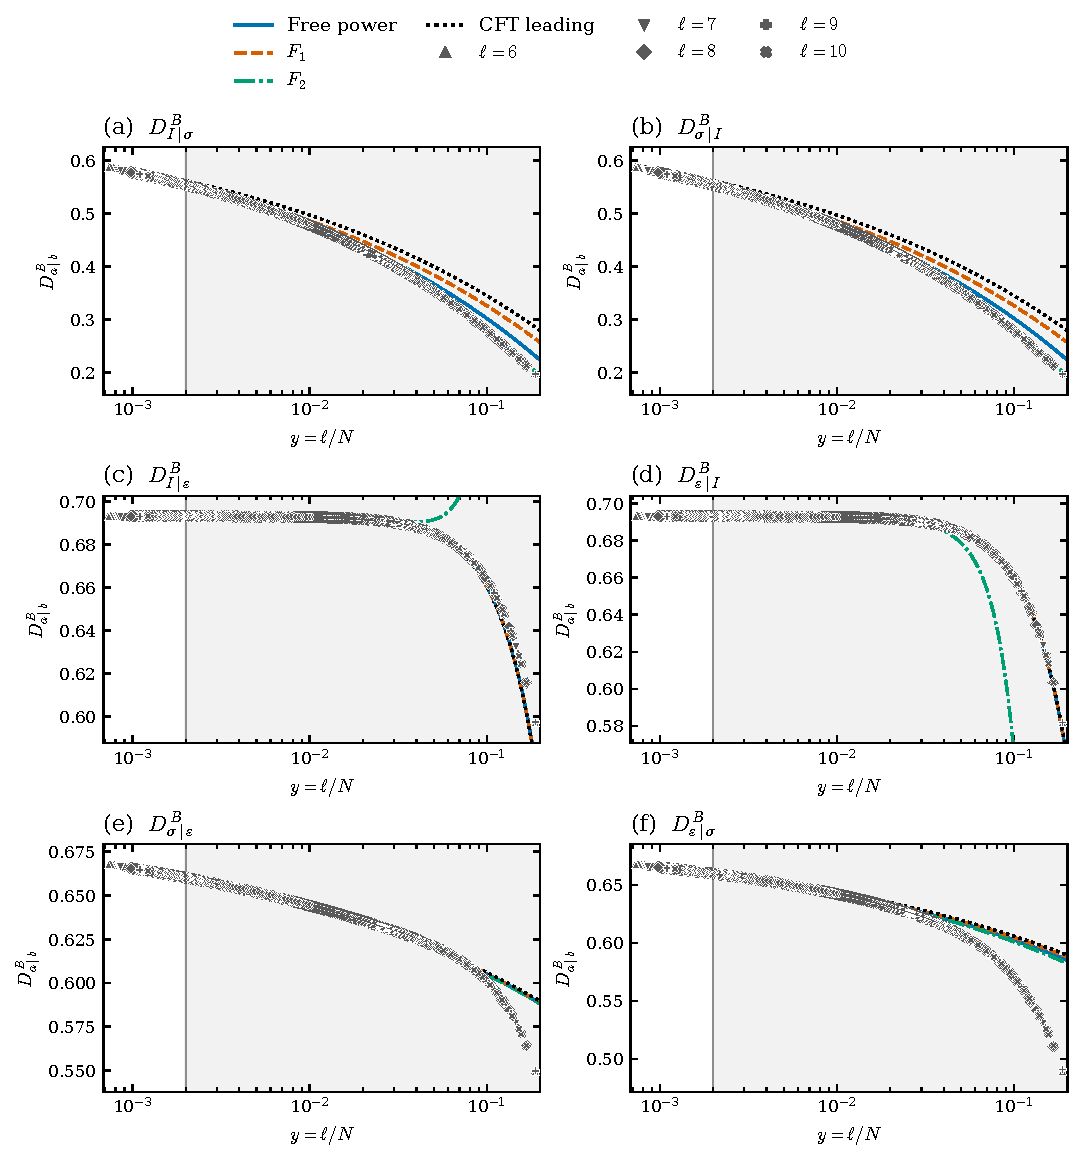
\includegraphics[width=.88\linewidth]{../figs/ising_large_entropy.pdf}
\caption{The ordinate is $D^B=\log2-\delta$, on a linear scale; tick labels give its value directly, without an additive offset. The fraction axis is logarithmic. Ising mixtures at $p=1/2$, $\ell=6,7,8,9,10$, and the chain-size set in Eq.~\eqref{eq:extended-grid}, with $32\leq N\leq8192$. There are 1645 displayed geometries per direction at $y\leq0.2$, of which 260 satisfy $y\leq0.002$ and enter every fit. Marker shape identifies $\ell$; the vertical boundary and gray shading mark the fitting cutoff and excluded data. The periodic Ising Hamiltonian is $H=-\sum_jX_jX_{j+1}-\sum_jZ_j$; primaries use exact fermionic covariances, including the odd Ramond ground state for $\sigma$. Natural logarithms apply. Added sizes use the direct entropy remainder in Sec.~\ref{sec:stable-entropy}, with support cutoff $10^{-15}$. Blue solid is the free-power fit (two fitted parameters), orange dashed is $F_1$ (one), green dash--dot is $F_2$ (two), and black dotted is the analytical CFT leading term (zero). Powers and amplitudes use Eqs.~\eqref{eq:fit} and \eqref{eq:complement-fit}; all coefficients include powers of $\pi$. Fits minimize unweighted squared residuals in $\delta$. These curves use \texttt{scaling\_fit\_summary.csv}. The identical fits in Tables~\ref{tab:ising-large-parameters} and \ref{tab:ising-large-metrics} also have per-pair full-range and fitting-window views in Sec.~\ref{sec:pair-large_ising}.}
\label{fig:ising-complement-entropy}
\end{figure}

\begin{figure}[p]\centering
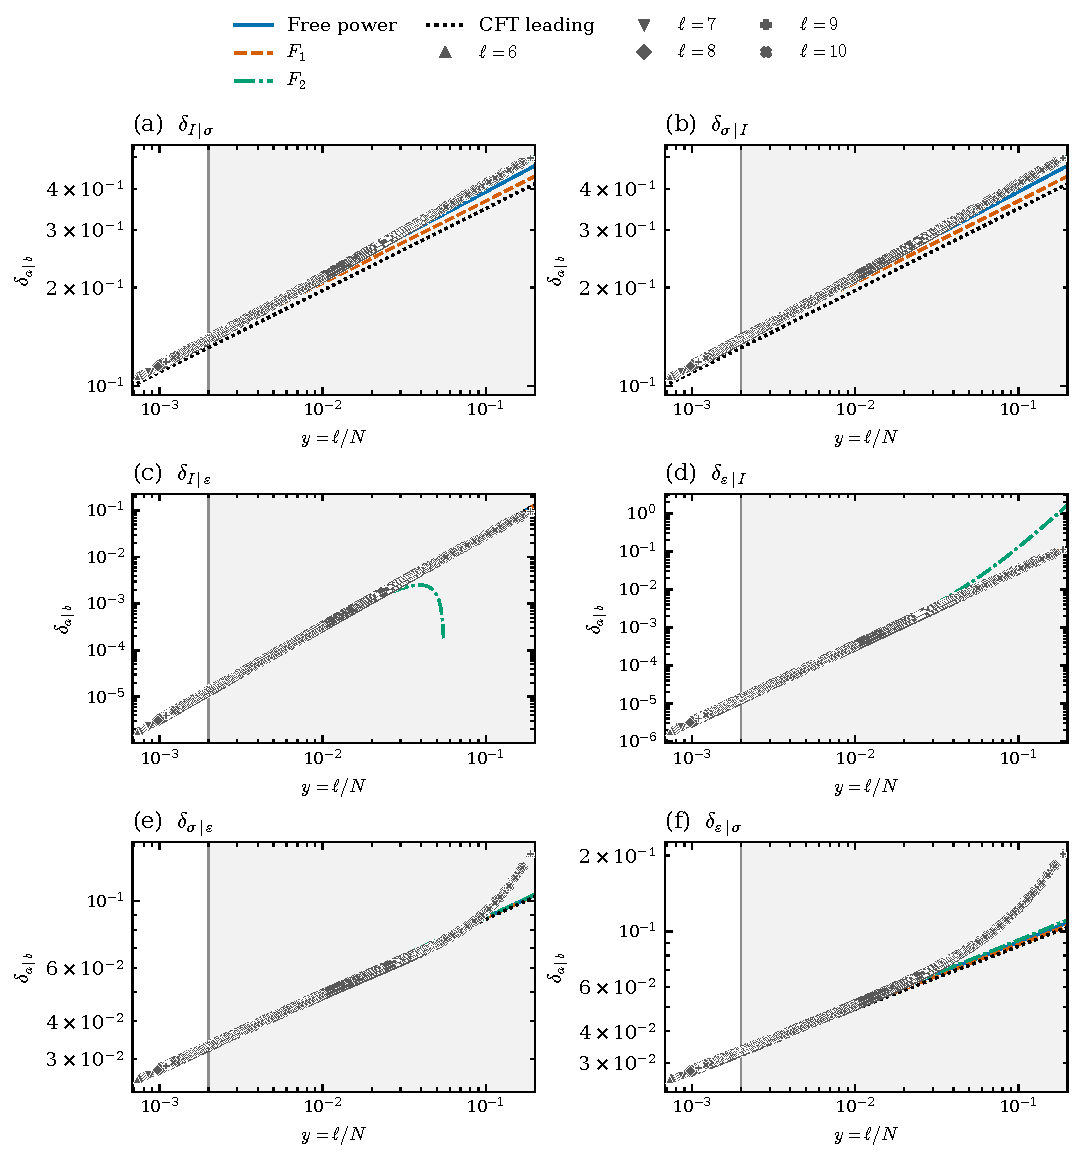
\includegraphics[width=.88\linewidth]{../figs/ising_large_value.pdf}
\caption{Both axes are logarithmic. Nonpositive values of an extrapolated truncated curve are omitted only from this logarithmic panel, while residual panels retain their predictions. Ising mixtures at $p=1/2$, $\ell=6,7,8,9,10$, and the chain-size set in Eq.~\eqref{eq:extended-grid}, with $32\leq N\leq8192$. There are 1645 displayed geometries per direction at $y\leq0.2$, of which 260 satisfy $y\leq0.002$ and enter every fit. Marker shape identifies $\ell$; the vertical boundary and gray shading mark the fitting cutoff and excluded data. The periodic Ising Hamiltonian is $H=-\sum_jX_jX_{j+1}-\sum_jZ_j$; primaries use exact fermionic covariances, including the odd Ramond ground state for $\sigma$. Natural logarithms apply. Added sizes use the direct entropy remainder in Sec.~\ref{sec:stable-entropy}, with support cutoff $10^{-15}$. Blue solid is the free-power fit (two fitted parameters), orange dashed is $F_1$ (one), green dash--dot is $F_2$ (two), and black dotted is the analytical CFT leading term (zero). Powers and amplitudes use Eqs.~\eqref{eq:fit} and \eqref{eq:complement-fit}; all coefficients include powers of $\pi$. Fits minimize unweighted squared residuals in $\delta$. These curves use \texttt{scaling\_fit\_summary.csv}. The identical fits in Tables~\ref{tab:ising-large-parameters} and \ref{tab:ising-large-metrics} also have per-pair full-range and fitting-window views in Sec.~\ref{sec:pair-large_ising}.}
\label{fig:ising-complement-deficit}
\end{figure}

\begin{figure}[p]\centering
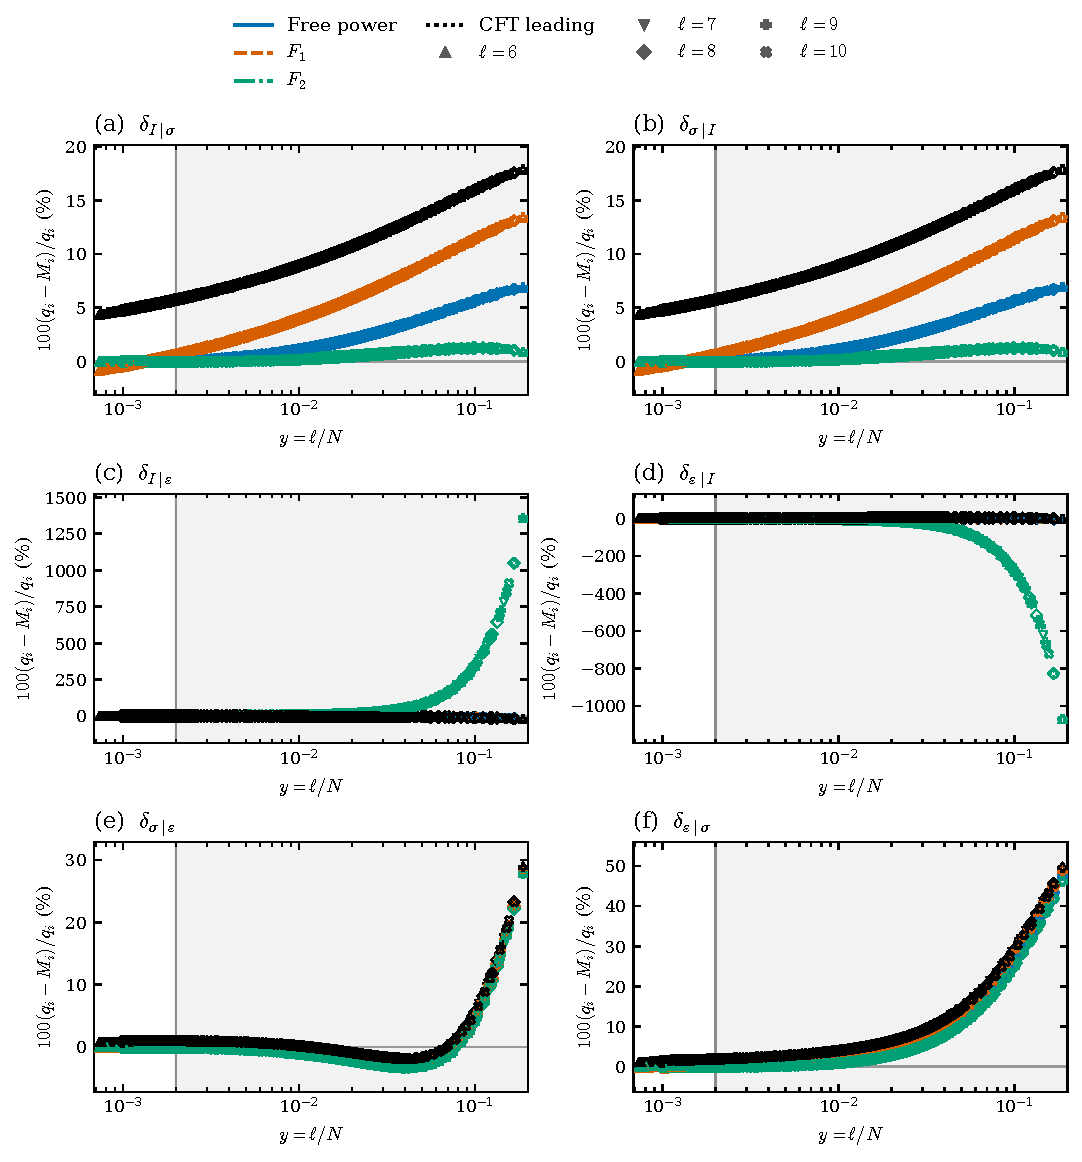
\includegraphics[width=.88\linewidth]{../figs/ising_large_residual.pdf}
\caption{The ordinate is $100(q_i-M_i)/q_i$ percent, with $q_i=D^A_i$ for a small interval and $q_i=\delta_i$ for a large interval; the horizontal zero line aids comparison. All four models have residual markers, colored as their curves. The residual ordinate is linear; the fraction axis is logarithmic. Ising mixtures at $p=1/2$, $\ell=6,7,8,9,10$, and the chain-size set in Eq.~\eqref{eq:extended-grid}, with $32\leq N\leq8192$. There are 1645 displayed geometries per direction at $y\leq0.2$, of which 260 satisfy $y\leq0.002$ and enter every fit. Marker shape identifies $\ell$; the vertical boundary and gray shading mark the fitting cutoff and excluded data. The periodic Ising Hamiltonian is $H=-\sum_jX_jX_{j+1}-\sum_jZ_j$; primaries use exact fermionic covariances, including the odd Ramond ground state for $\sigma$. Natural logarithms apply. Added sizes use the direct entropy remainder in Sec.~\ref{sec:stable-entropy}, with support cutoff $10^{-15}$. Blue solid is the free-power fit (two fitted parameters), orange dashed is $F_1$ (one), green dash--dot is $F_2$ (two), and black dotted is the analytical CFT leading term (zero). Powers and amplitudes use Eqs.~\eqref{eq:fit} and \eqref{eq:complement-fit}; all coefficients include powers of $\pi$. Fits minimize unweighted squared residuals in $\delta$. These curves use \texttt{scaling\_fit\_summary.csv}. The identical fits in Tables~\ref{tab:ising-large-parameters} and \ref{tab:ising-large-metrics} also have per-pair full-range and fitting-window views in Sec.~\ref{sec:pair-large_ising}.}
\label{fig:ising-complement-residuals}
\end{figure}

\begin{figure}[p]\centering
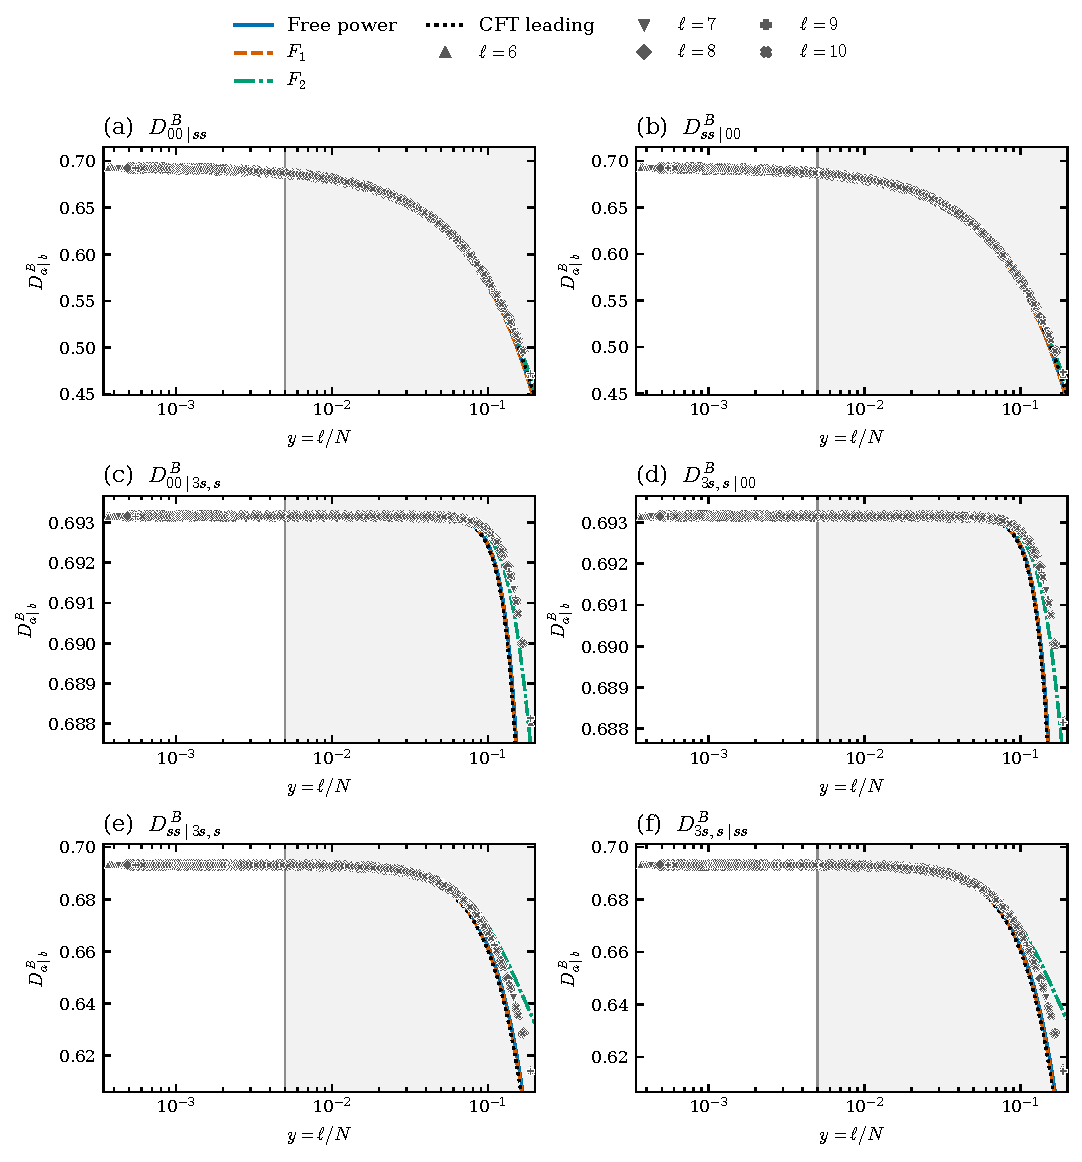
\includegraphics[width=.88\linewidth]{../figs/boson_large_entropy.pdf}
\caption{The ordinate is $D^B=\log2-\delta$, on a linear scale; tick labels give its value directly, without an additive offset. The fraction axis is logarithmic. Compact-boson mixtures at $p=1/2$, $\ell=6,7,8,9,10$, and the chain-size set in Eq.~\eqref{eq:extended-grid}, with $32\leq N\leq16384$. There are 625 displayed geometries per direction at $y\leq0.2$, of which 317 satisfy $y\leq0.005$ and enter every fit. Marker shape identifies $\ell$; the vertical boundary and gray shading mark the fitting cutoff and excluded data. The boson uses $s=1/\sqrt2$, $q=2$, charge codes $(0,0),(1,1),(3,1)$, $z_j=e^{2\pi i j/N}$, $w_1=0$, and $W=10^8$; moment algebra uses 100 digits through $N=256$ and 120 digits at the added sizes. Natural logarithms apply. Added sizes use the direct entropy remainder in Sec.~\ref{sec:stable-entropy}, with support cutoff $10^{-15}$. Blue solid is the free-power fit (two fitted parameters), orange dashed is $F_1$ (one), green dash--dot is $F_2$ (two), and black dotted is the analytical CFT leading term (zero). Powers and amplitudes use Eqs.~\eqref{eq:fit} and \eqref{eq:complement-fit}; all coefficients include powers of $\pi$. Fits minimize unweighted squared residuals in $\delta$. These curves use \texttt{scaling\_fit\_summary.csv}. The identical fits in Tables~\ref{tab:boson-large-parameters} and \ref{tab:boson-large-metrics} also have per-pair full-range and fitting-window views in Sec.~\ref{sec:pair-large_boson}.}
\label{fig:boson-complement-entropy}
\end{figure}

\begin{figure}[p]\centering
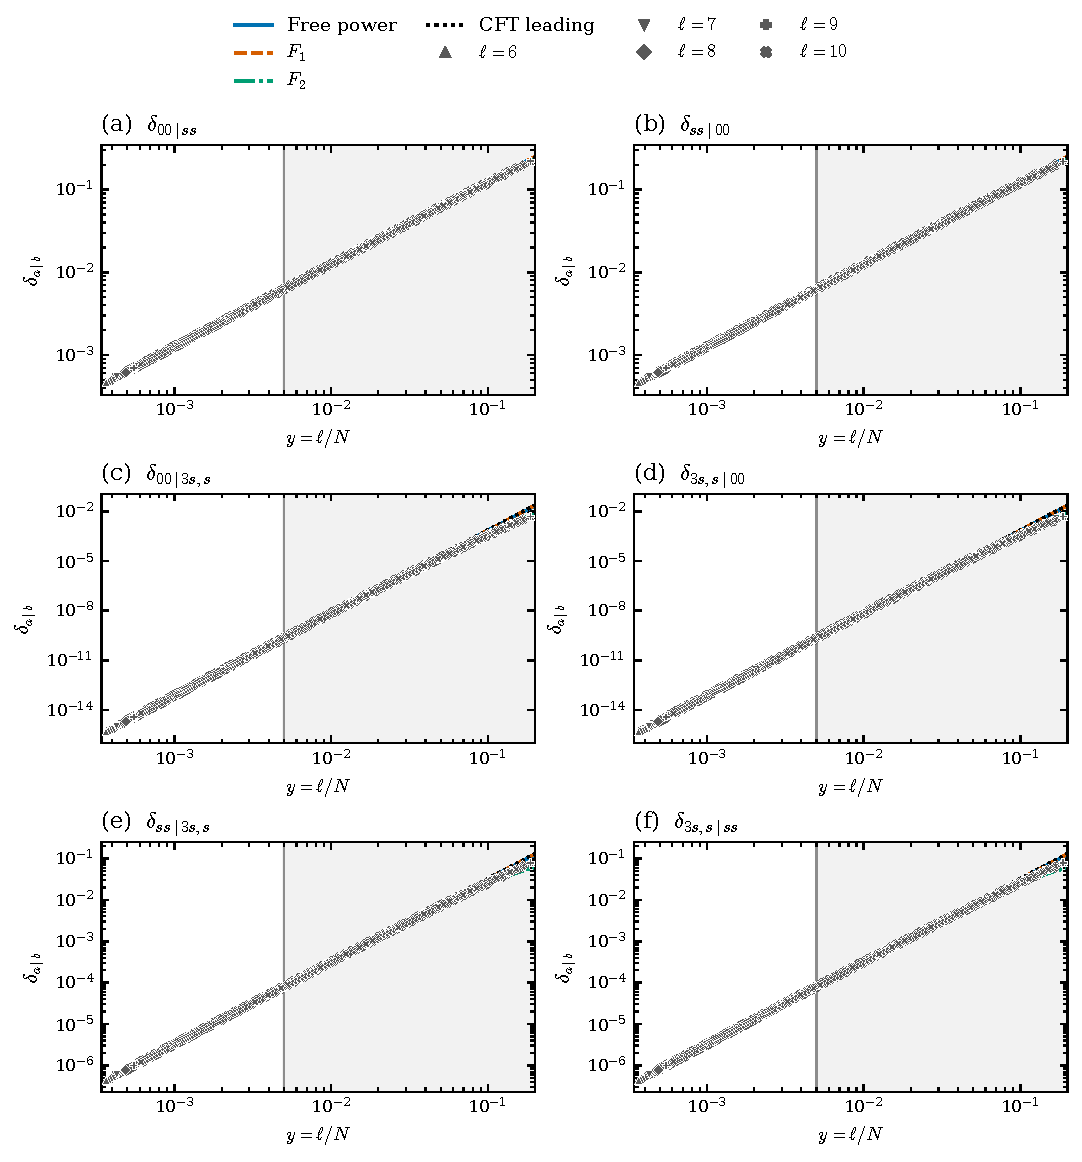
\includegraphics[width=.88\linewidth]{../figs/boson_large_value.pdf}
\caption{Both axes are logarithmic. Nonpositive values of an extrapolated truncated curve are omitted only from this logarithmic panel, while residual panels retain their predictions. Compact-boson mixtures at $p=1/2$, $\ell=6,7,8,9,10$, and the chain-size set in Eq.~\eqref{eq:extended-grid}, with $32\leq N\leq16384$. There are 625 displayed geometries per direction at $y\leq0.2$, of which 317 satisfy $y\leq0.005$ and enter every fit. Marker shape identifies $\ell$; the vertical boundary and gray shading mark the fitting cutoff and excluded data. The boson uses $s=1/\sqrt2$, $q=2$, charge codes $(0,0),(1,1),(3,1)$, $z_j=e^{2\pi i j/N}$, $w_1=0$, and $W=10^8$; moment algebra uses 100 digits through $N=256$ and 120 digits at the added sizes. Natural logarithms apply. Added sizes use the direct entropy remainder in Sec.~\ref{sec:stable-entropy}, with support cutoff $10^{-15}$. Blue solid is the free-power fit (two fitted parameters), orange dashed is $F_1$ (one), green dash--dot is $F_2$ (two), and black dotted is the analytical CFT leading term (zero). Powers and amplitudes use Eqs.~\eqref{eq:fit} and \eqref{eq:complement-fit}; all coefficients include powers of $\pi$. Fits minimize unweighted squared residuals in $\delta$. These curves use \texttt{scaling\_fit\_summary.csv}. The identical fits in Tables~\ref{tab:boson-large-parameters} and \ref{tab:boson-large-metrics} also have per-pair full-range and fitting-window views in Sec.~\ref{sec:pair-large_boson}.}
\label{fig:boson-complement-deficit}
\end{figure}

\begin{figure}[p]\centering
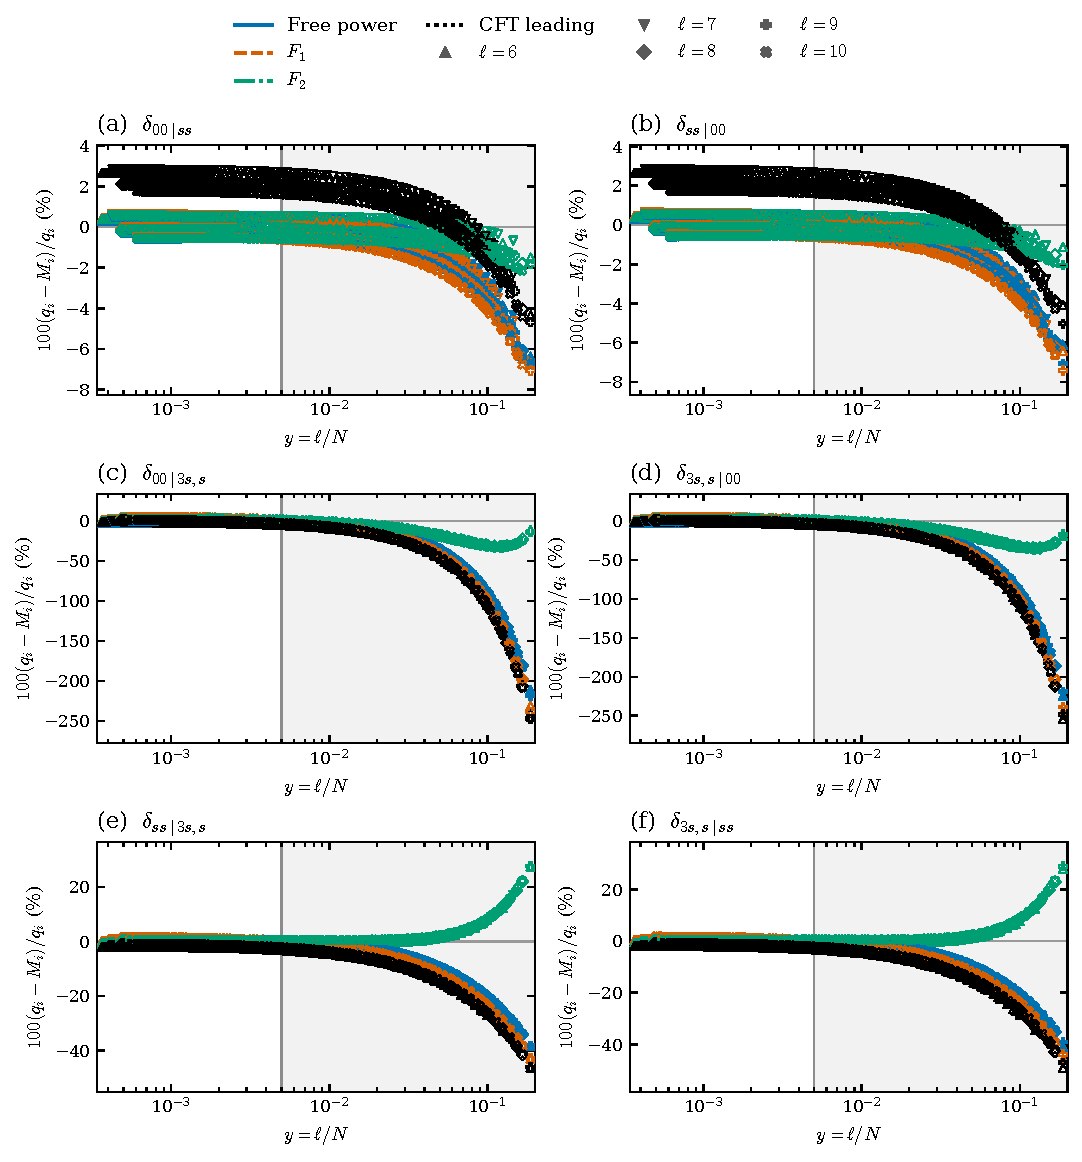
\includegraphics[width=.88\linewidth]{../figs/boson_large_residual.pdf}
\caption{The ordinate is $100(q_i-M_i)/q_i$ percent, with $q_i=D^A_i$ for a small interval and $q_i=\delta_i$ for a large interval; the horizontal zero line aids comparison. All four models have residual markers, colored as their curves. The residual ordinate is linear; the fraction axis is logarithmic. Compact-boson mixtures at $p=1/2$, $\ell=6,7,8,9,10$, and the chain-size set in Eq.~\eqref{eq:extended-grid}, with $32\leq N\leq16384$. There are 625 displayed geometries per direction at $y\leq0.2$, of which 317 satisfy $y\leq0.005$ and enter every fit. Marker shape identifies $\ell$; the vertical boundary and gray shading mark the fitting cutoff and excluded data. The boson uses $s=1/\sqrt2$, $q=2$, charge codes $(0,0),(1,1),(3,1)$, $z_j=e^{2\pi i j/N}$, $w_1=0$, and $W=10^8$; moment algebra uses 100 digits through $N=256$ and 120 digits at the added sizes. Natural logarithms apply. Added sizes use the direct entropy remainder in Sec.~\ref{sec:stable-entropy}, with support cutoff $10^{-15}$. Blue solid is the free-power fit (two fitted parameters), orange dashed is $F_1$ (one), green dash--dot is $F_2$ (two), and black dotted is the analytical CFT leading term (zero). Powers and amplitudes use Eqs.~\eqref{eq:fit} and \eqref{eq:complement-fit}; all coefficients include powers of $\pi$. Fits minimize unweighted squared residuals in $\delta$. These curves use \texttt{scaling\_fit\_summary.csv}. The identical fits in Tables~\ref{tab:boson-large-parameters} and \ref{tab:boson-large-metrics} also have per-pair full-range and fitting-window views in Sec.~\ref{sec:pair-large_boson}.}
\label{fig:boson-complement-residuals}
\end{figure}



\clearpage
\section{Visual comparison of fits for each ordered pair}
\label{sec:window-selection}
\subsection{Question, data, and models}
For each ordered pair we display the fitting models, their actual
intervals, their residuals, and the supplied analytical curve together.
Each figure compares the principal summary-table fits in its left column
with the varying-window fits in its right column. We compare Free 1,
$F_1$, and $F_2$. Each column uses one common interval for all three
models, so adding the second term can be assessed on identical observations.

We use every previously computed mixture geometry in
Eq.~\eqref{eq:extended-grid}, with $p=1/2$ and $\ell=6,\ldots,10$.
The raw $\ell=4,5$ observations remain archived but enter neither estimation nor display.
This restores the five-length analysis on its original chain grid;
the subsequent $\ell=11,12$ extension and complete-seven-length-block
study remain separate archived comparisons. In the current analysis,
each observation with $\ell\in\{6,7,8,9,10\}$ is selected individually
using its fraction $\ell/N$ and the group's fitting window; a size need
not contribute every length inside that window.
The dense scan adds 235 Ising and 47 boson sizes, all below the previously validated maxima; see Appendix~\ref{sec:dense-second-order}. Write $z=x=\ell/N$
and $q=D^A$ for small intervals; write $z=y=\ell/N$ and
$q=\delta=\log2-D^B$ for large complementary intervals. Thus $\alpha$
always denotes a small-interval leading power and $\beta$ a
large-interval leading power. All active models use the four common windows in
Eq.~\eqref{eq:common-fit-windows}; the small-interval choices are
frozen and the large-boson upper cutoff is prescribed as $0.005$.
The same fits appear in the overview figures and the principal
tables in Appendices~\ref{sec:allfits} and \ref{sec:complement-checks}.
The earlier $(0,0.001]$ free-power fits remain a separate diagnostic.

For a window $W=[u,v]$, we compare
\begin{align}
 F_1(z)&=c_1z^{r_0},&
 F_{\mathrm{free},1}(z)&=c_1z^{r^{(1)}},\nonumber\\
 F_2(z)&=c_1z^{r_0}+c_2z^{r_{\rm next}}.
 \label{eq:window-models}
\end{align}
Here $r_0,r_{\rm next}$ are the pair-specific manuscript powers;
$F_2$ fixes both, since a general separation between freely estimated
leading and next powers is not established. Free 1 estimates only the
leading power. In this section $c_1$ is the leading amplitude and $c_2$ the
next amplitude, corresponding to $c_0,c_1$ in
Eq.~\eqref{eq:fit}. They multiply $z^r$ itself and include all powers
of $\pi$. There are one, two, and two fitted parameters in
$F_1$, Free 1, and $F_2$, respectively. The objective is always
\begin{equation}
 \mathrm{SSE}_W=\sum_{i:z_i\in W}[q_i-M(z_i)]^2.
 \label{eq:window-objective}
\end{equation}
All geometries receive equal weight, including distinct $(N,\ell)$
that have the same fraction. No logarithmic residual objective or
extra lattice-correction term is fitted.

The theory comparison uses the source
\texttt{manuscript\_theory/main3.tex}~\cite{theoryLarge}, especially its
non-chiral compact-boson and Ising examples. The small-interval powers
and complete supplied coefficients are in
Tables~\ref{tab:isingcoeff} and \ref{tab:bosoncoeff}:
$r_{\rm next}=\alpha+2$. Only $I\mid\eps$ and $\eps\mid I$ have
complete supplied next coefficients. Large intervals use
Table~\ref{tab:complement-theory}; no common increment is assumed.
For large boson $ss\leftrightarrow3s,s$, power three is an allowed
sector, not a proved nonzero coefficient. An empty analytical cell
in the new tables means that the complete coefficient is unavailable.

\subsection{Fitting formulas and plotted quantities}
For fixed powers, the coefficients follow from linear least squares.
Use $t_i=\log(z_i/v)$ and $A_j=c_jv^{r_j}$. Define
\begin{equation}
 X_{ij}=\exp(r_jt_i),\qquad
 \widehat{\boldsymbol A}=X^+\boldsymbol q,\qquad
 c_j=\widehat A_j/v^{r_j}.
 \label{eq:window-profile}
\end{equation}
$X^+$ is the Moore--Penrose pseudoinverse, computed by singular-value
decomposition. For $F_1$ the design matrix has one column with power
$r_0$; for $F_2$ it has two columns with powers $r_0,r_{\rm next}$.
Free 1 uses one column and minimizes the residual over its single
trial power. Eliminating the linear coefficient before this search
is variable projection~\cite{GolubPereyra}. Dividing all $q_i$ by their
root-mean-square value improves numerical scaling and does not change
the least-squares optimum.

In the figures, the upper panels show $q$ and the fitted curves.
Solid colored segments lie inside the corresponding interval $W$;
thin dotted segments show extrapolation. The lower residual panels
show only the observations used by each fit, with
$R_i=100[q_i-M(z_i)]/q_i$ on a linear ordinate. The interval bars and
parameter block specify $W$ separately for every model. A zero lower
endpoint is open; it includes the smallest positive observation.
The left column shows all available data through $z=0.20$; the
right column zooms into the common fitting window using the same
curves. Both residual columns show the same fitted observations on
linear ordinates. The shared parameter block lists each fit once.

For the numerical-error tables, define
\begin{equation}
 E_{\rm fit}=100\sqrt{\frac{\sum_{i\in W}[q_i-M(z_i)]^2}
                              {\sum_{i\in W}q_i^2}},\qquad
 E_{\rm CV}=100\sqrt{\frac{\sum_{i\in W}[q_i-M^{(-N_i)}(z_i)]^2}
                             {\sum_{i\in W}q_i^2}}.
 \label{eq:pair-errors}
\end{equation}
Here $M^{(-N_i)}$ is refitted after omitting all observations at chain
size $N_i$, as in Eq.~\eqref{eq:cv}. These aggregate percentages differ
from the pointwise percentages in the residual panels. Every displayed
fit and omitted-size training set contains at least forty observations.
Different fitting intervals contain different observations, so their
absolute RMSEs should not be ranked directly.

\subsection{Comparison with theory and results}
Compare the fitted parameters with the manuscript using
\begin{equation}
 \eta_{c,j}=100\left(\frac{c_j}{c_j^{\rm CFT}}-1\right),\qquad
 \eta_{r,j}=100\left(\frac{r^{(j)}}{r_j^{\rm CFT}}-1\right),
 \qquad j=1,2.
 \label{eq:window-discrepancies}
\end{equation}
An unknown analytical coefficient leaves both its comparison cell
and its percentage discrepancy empty. Fixed exponents are identified
as imposed rather than estimated. All models and all six directions within one CFT and interval type
use the same window. Both columns show the same fitted models. The current omitted-size
controls are in \path{data/f2_summary_cv.csv}; the principal-table gains
use Eq.~\eqref{eq:table-window-gains}.
The known small-Ising next coefficients provide a direct comparison: $F_2$ gives $c_2=-170.71,-355.38$ for $I\mid\eps$ and $\eps\mid I$, whereas the manuscript gives $-8\pi^6/45$ and $-8\pi^6/21$. The signed discrepancies are $-0.12\%,-2.97\%$. These fits use the common small-Ising window in both columns; Appendix~\ref{sec:dense-second-order} examines the stability of both coefficients. The tables retain every fitted value and compare all supplied theoretical powers and coefficients.\par

\begingroup\setlength{\tabcolsep}{2pt}
\begin{longtable}{lll}
\caption{Ising small intervals: fitting intervals for the models shown in the right-hand panels of Sec.~\ref{sec:pair-small_ising}. All three models share the displayed interval, providing an identical-data comparison. Zero is an open lower bound, with no observation at zero.}
\label{tab:window-small_ising-ranges}\\\toprule
Direction & Free 1 and $F_1$ & $F_2$\\\midrule
\endfirsthead
\toprule
Direction & Free 1 and $F_1$ & $F_2$\\\midrule
\endhead
\bottomrule\endfoot
$I\mid \sigma$ & $(0,0.02]$ & $(0,0.02]$\\
$\sigma\mid I$ & $(0,0.02]$ & $(0,0.02]$\\
$I\mid \varepsilon$ & $(0,0.02]$ & $(0,0.02]$\\
$\varepsilon\mid I$ & $(0,0.02]$ & $(0,0.02]$\\
$\sigma\mid \varepsilon$ & $(0,0.02]$ & $(0,0.02]$\\
$\varepsilon\mid \sigma$ & $(0,0.02]$ & $(0,0.02]$\\
\end{longtable}
\endgroup

\begingroup\setlength{\tabcolsep}{2pt}
\begin{longtable}{lll}
\caption{Compact boson small intervals: fitting intervals for the models shown in the right-hand panels of Sec.~\ref{sec:pair-small_boson}. All three models share the displayed interval, providing an identical-data comparison. Zero is an open lower bound, with no observation at zero.}
\label{tab:window-small_boson-ranges}\\\toprule
Direction & Free 1 and $F_1$ & $F_2$\\\midrule
\endfirsthead
\toprule
Direction & Free 1 and $F_1$ & $F_2$\\\midrule
\endhead
\bottomrule\endfoot
$00\mid ss$ & $(0,0.1]$ & $(0,0.1]$\\
$ss\mid 00$ & $(0,0.1]$ & $(0,0.1]$\\
$00\mid 3s,s$ & $(0,0.1]$ & $(0,0.1]$\\
$3s,s\mid 00$ & $(0,0.1]$ & $(0,0.1]$\\
$ss\mid 3s,s$ & $(0,0.1]$ & $(0,0.1]$\\
$3s,s\mid ss$ & $(0,0.1]$ & $(0,0.1]$\\
\end{longtable}
\endgroup

\begingroup\setlength{\tabcolsep}{2pt}
\begin{longtable}{lll}
\caption{Ising large intervals: fitting intervals for the models shown in the right-hand panels of Sec.~\ref{sec:pair-large_ising}. All three models share the displayed interval, providing an identical-data comparison. Zero is an open lower bound, with no observation at zero.}
\label{tab:window-large_ising-ranges}\\\toprule
Direction & Free 1 and $F_1$ & $F_2$\\\midrule
\endfirsthead
\toprule
Direction & Free 1 and $F_1$ & $F_2$\\\midrule
\endhead
\bottomrule\endfoot
$I\mid \sigma$ & $(0,0.002]$ & $(0,0.002]$\\
$\sigma\mid I$ & $(0,0.002]$ & $(0,0.002]$\\
$I\mid \varepsilon$ & $(0,0.002]$ & $(0,0.002]$\\
$\varepsilon\mid I$ & $(0,0.002]$ & $(0,0.002]$\\
$\sigma\mid \varepsilon$ & $(0,0.002]$ & $(0,0.002]$\\
$\varepsilon\mid \sigma$ & $(0,0.002]$ & $(0,0.002]$\\
\end{longtable}
\endgroup

\begingroup\setlength{\tabcolsep}{2pt}
\begin{longtable}{lll}
\caption{Compact boson large intervals: fitting intervals for the models shown in the right-hand panels of Sec.~\ref{sec:pair-large_boson}. All three models share the displayed interval, providing an identical-data comparison. Zero is an open lower bound, with no observation at zero.}
\label{tab:window-large_boson-ranges}\\\toprule
Direction & Free 1 and $F_1$ & $F_2$\\\midrule
\endfirsthead
\toprule
Direction & Free 1 and $F_1$ & $F_2$\\\midrule
\endhead
\bottomrule\endfoot
$00\mid ss$ & $(0,0.005]$ & $(0,0.005]$\\
$ss\mid 00$ & $(0,0.005]$ & $(0,0.005]$\\
$00\mid 3s,s$ & $(0,0.005]$ & $(0,0.005]$\\
$3s,s\mid 00$ & $(0,0.005]$ & $(0,0.005]$\\
$ss\mid 3s,s$ & $(0,0.005]$ & $(0,0.005]$\\
$3s,s\mid ss$ & $(0,0.005]$ & $(0,0.005]$\\
\end{longtable}
\endgroup

The full amplitudes, powers, and theoretical comparisons are in
Appendix~\ref{sec:window-appendix}. Each figure below treats one
ordered pair. Its parameter block lists every displayed fit and the common window
used in both columns. Window sensitivity is examined separately in
Appendix~\ref{sec:dense-second-order}.
The analytical curve has no fitted
parameters. All retained-model results remain visible without window
classifications or acceptance labels.
\clearpage
\subsection{Ising, small intervals}
\label{sec:pair-small_ising}
\begin{figure}[!htbp]\centering
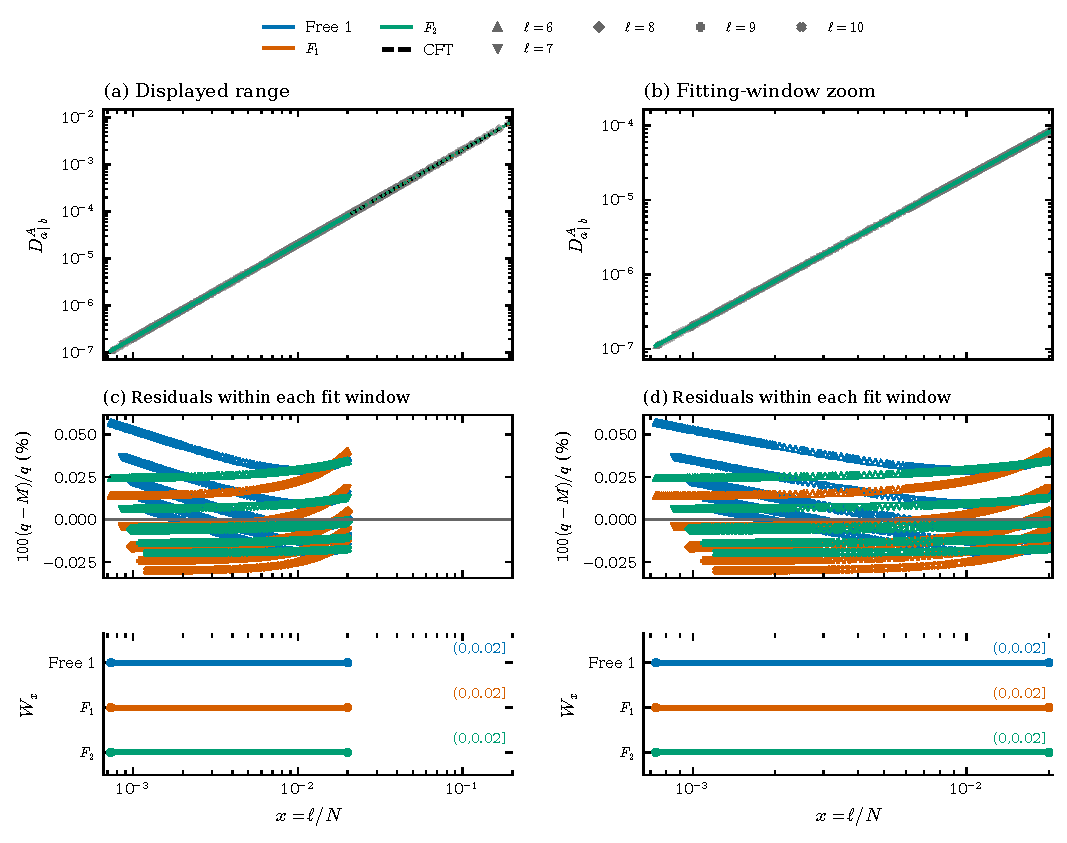
\includegraphics[width=.94\linewidth]{../figs/pair_small_ising_I_sigma.pdf}\par\smallskip
\begingroup\scriptsize\setlength{\tabcolsep}{4pt}
\begin{tabular}{lllrrrrr}\toprule
Set & Model & $W_z$ & $m$ & $c_0$ & $r^{(0)}$ & $c_1$ & $r^{(1)}$\\\midrule
Both & Free 1 & $(0,0.02]$ & 1255 & 0.20585 & 2.0001419 & --- & ---\\
Both & $F_1$ & $(0,0.02]$ & 1255 & 0.20573 & 2 & --- & ---\\
Both & $F_2$ & $(0,0.02]$ & 1255 & 0.20571 & 2 & 0.083833 & 4\\
\midrule
Both & CFT & --- & --- & 0.20562 & 2 & --- & ---\\
\bottomrule\end{tabular}
\endgroup
\caption{Ising, small intervals, $I\mid \sigma$, at $p=1/2$, $\ell=6,\ldots,10$, and the complete size grid in Eq.~\eqref{eq:extended-grid}. Here $z=x$ and $q=D^A$. Left: all computed data through $z=0.20$; right: a zoom into the common fitting window. Both columns show the same Free 1, $F_1$, and $F_2$ fits. All six directions of this CFT and interval type use the same window. Gray markers denote the data. Colored solid segments lie inside each model\textquotesingle s fitting interval; dotted segments are extrapolations. Black dashed is the supplied CFT series. The observable axes are logarithmic and span the measured data; nonpositive predictions cannot appear there and out-of-range extrapolations leave the panel. Residual ordinates are linear and show $100(q-M)/q$ only on each model\textquotesingle s fitted observations. Bars give the exact fitting intervals. The parameter block follows Eq.~\eqref{eq:fit}, with $c_0,c_1$ multiplying $z^{r^{(0)}},z^{r^{(1)}}$; all coefficients include powers of $\pi$. A dash means an absent fitted term, or no fitting window for CFT. Values shown are rounded; curves use full precision.}
\label{fig:pair-small_ising-I-sigma}
\end{figure}
\begin{figure}[!htbp]\centering
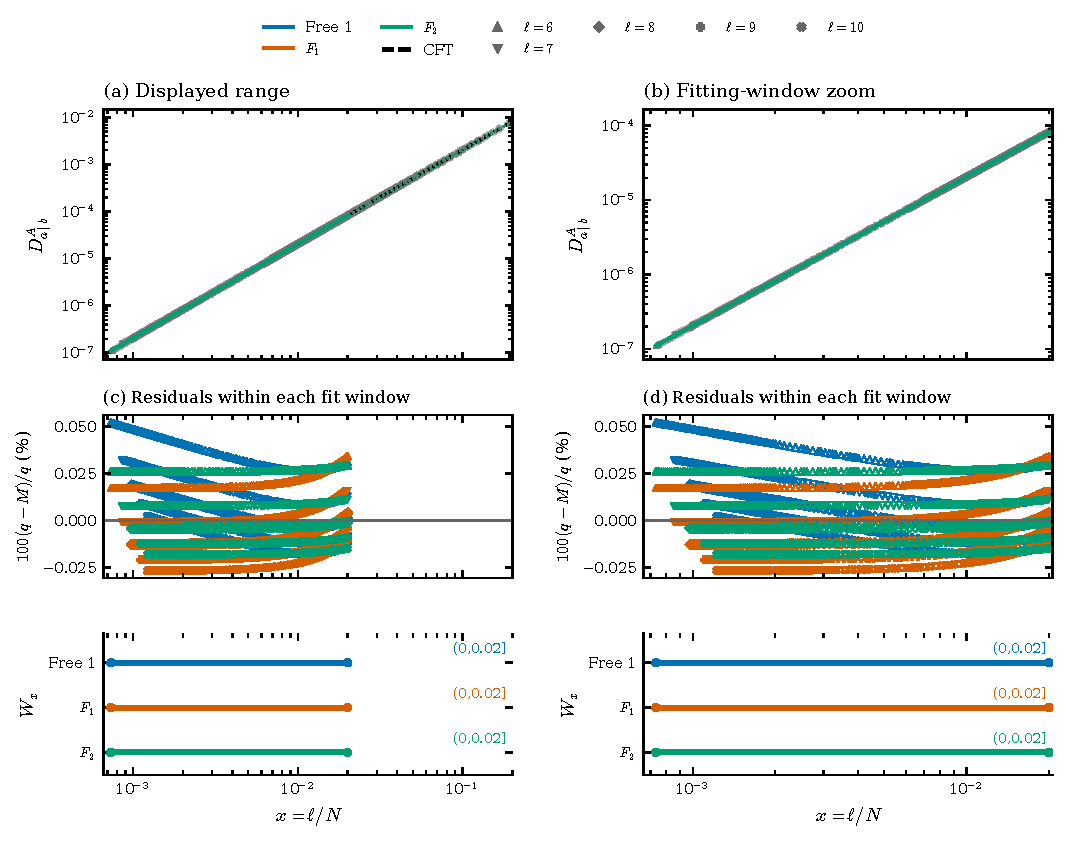
\includegraphics[width=.94\linewidth]{../figs/pair_small_ising_sigma_I.pdf}\par\smallskip
\begingroup\scriptsize\setlength{\tabcolsep}{4pt}
\begin{tabular}{lllrrrrr}\toprule
Set & Model & $W_z$ & $m$ & $c_0$ & $r^{(0)}$ & $c_1$ & $r^{(1)}$\\\midrule
Both & Free 1 & $(0,0.02]$ & 1255 & 0.20582 & 2.0001141 & --- & ---\\
Both & $F_1$ & $(0,0.02]$ & 1255 & 0.20572 & 2 & --- & ---\\
Both & $F_2$ & $(0,0.02]$ & 1255 & 0.2057 & 2 & 0.069099 & 4\\
\midrule
Both & CFT & --- & --- & 0.20562 & 2 & --- & ---\\
\bottomrule\end{tabular}
\endgroup
\caption{Ising, small intervals, $\sigma\mid I$, at $p=1/2$, $\ell=6,\ldots,10$, and the complete size grid in Eq.~\eqref{eq:extended-grid}. Here $z=x$ and $q=D^A$. Left: all computed data through $z=0.20$; right: a zoom into the common fitting window. Both columns show the same Free 1, $F_1$, and $F_2$ fits. All six directions of this CFT and interval type use the same window. Gray markers denote the data. Colored solid segments lie inside each model\textquotesingle s fitting interval; dotted segments are extrapolations. Black dashed is the supplied CFT series. The observable axes are logarithmic and span the measured data; nonpositive predictions cannot appear there and out-of-range extrapolations leave the panel. Residual ordinates are linear and show $100(q-M)/q$ only on each model\textquotesingle s fitted observations. Bars give the exact fitting intervals. The parameter block follows Eq.~\eqref{eq:fit}, with $c_0,c_1$ multiplying $z^{r^{(0)}},z^{r^{(1)}}$; all coefficients include powers of $\pi$. A dash means an absent fitted term, or no fitting window for CFT. Values shown are rounded; curves use full precision.}
\label{fig:pair-small_ising-sigma-I}
\end{figure}
\begin{figure}[!htbp]\centering
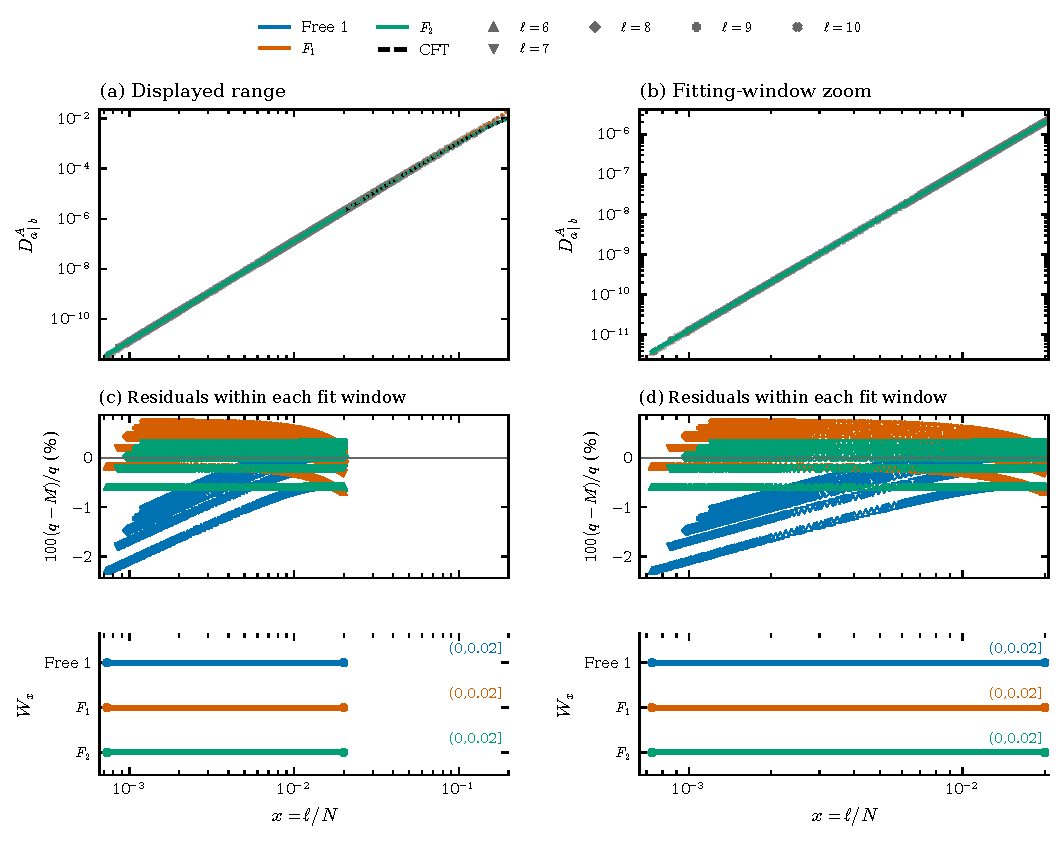
\includegraphics[width=.94\linewidth]{../figs/pair_small_ising_I_epsilon.pdf}\par\smallskip
\begingroup\scriptsize\setlength{\tabcolsep}{4pt}
\begin{tabular}{lllrrrrr}\toprule
Set & Model & $W_z$ & $m$ & $c_0$ & $r^{(0)}$ & $c_1$ & $r^{(1)}$\\\midrule
Both & Free 1 & $(0,0.02]$ & 1255 & 12.491 & 3.9933972 & --- & ---\\
Both & $F_1$ & $(0,0.02]$ & 1255 & 12.83 & 4 & --- & ---\\
Both & $F_2$ & $(0,0.02]$ & 1255 & 12.883 & 4 & -170.71 & 6\\
\midrule
Both & CFT & --- & --- & 12.988 & 4 & -170.91 & 6\\
\bottomrule\end{tabular}
\endgroup
\caption{Ising, small intervals, $I\mid \varepsilon$, at $p=1/2$, $\ell=6,\ldots,10$, and the complete size grid in Eq.~\eqref{eq:extended-grid}. Here $z=x$ and $q=D^A$. Left: all computed data through $z=0.20$; right: a zoom into the common fitting window. Both columns show the same Free 1, $F_1$, and $F_2$ fits. All six directions of this CFT and interval type use the same window. Gray markers denote the data. Colored solid segments lie inside each model\textquotesingle s fitting interval; dotted segments are extrapolations. Black dashed is the supplied CFT series. The observable axes are logarithmic and span the measured data; nonpositive predictions cannot appear there and out-of-range extrapolations leave the panel. Residual ordinates are linear and show $100(q-M)/q$ only on each model\textquotesingle s fitted observations. Bars give the exact fitting intervals. The parameter block follows Eq.~\eqref{eq:fit}, with $c_0,c_1$ multiplying $z^{r^{(0)}},z^{r^{(1)}}$; all coefficients include powers of $\pi$. A dash means an absent fitted term, or no fitting window for CFT. Values shown are rounded; curves use full precision.}
\label{fig:pair-small_ising-I-epsilon}
\end{figure}
\begin{figure}[!htbp]\centering
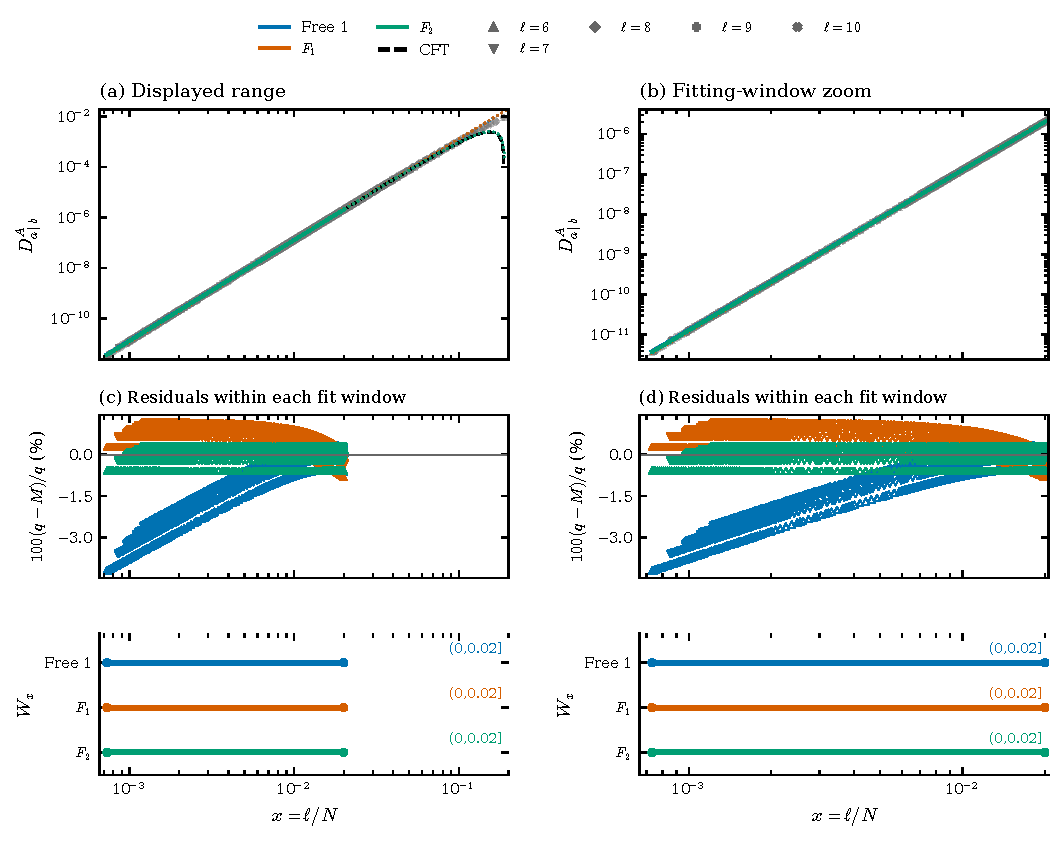
\includegraphics[width=.94\linewidth]{../figs/pair_small_ising_epsilon_I.pdf}\par\smallskip
\begingroup\scriptsize\setlength{\tabcolsep}{4pt}
\begin{tabular}{lllrrrrr}\toprule
Set & Model & $W_z$ & $m$ & $c_0$ & $r^{(0)}$ & $c_1$ & $r^{(1)}$\\\midrule
Both & Free 1 & $(0,0.02]$ & 1255 & 12.07 & 3.9860672 & --- & ---\\
Both & $F_1$ & $(0,0.02]$ & 1255 & 12.77 & 4 & --- & ---\\
Both & $F_2$ & $(0,0.02]$ & 1255 & 12.882 & 4 & -355.38 & 6\\
\midrule
Both & CFT & --- & --- & 12.988 & 4 & -366.24 & 6\\
\bottomrule\end{tabular}
\endgroup
\caption{Ising, small intervals, $\varepsilon\mid I$, at $p=1/2$, $\ell=6,\ldots,10$, and the complete size grid in Eq.~\eqref{eq:extended-grid}. Here $z=x$ and $q=D^A$. Left: all computed data through $z=0.20$; right: a zoom into the common fitting window. Both columns show the same Free 1, $F_1$, and $F_2$ fits. All six directions of this CFT and interval type use the same window. Gray markers denote the data. Colored solid segments lie inside each model\textquotesingle s fitting interval; dotted segments are extrapolations. Black dashed is the supplied CFT series. The observable axes are logarithmic and span the measured data; nonpositive predictions cannot appear there and out-of-range extrapolations leave the panel. Residual ordinates are linear and show $100(q-M)/q$ only on each model\textquotesingle s fitted observations. Bars give the exact fitting intervals. The parameter block follows Eq.~\eqref{eq:fit}, with $c_0,c_1$ multiplying $z^{r^{(0)}},z^{r^{(1)}}$; all coefficients include powers of $\pi$. A dash means an absent fitted term, or no fitting window for CFT. Values shown are rounded; curves use full precision.}
\label{fig:pair-small_ising-epsilon-I}
\end{figure}
\begin{figure}[!htbp]\centering
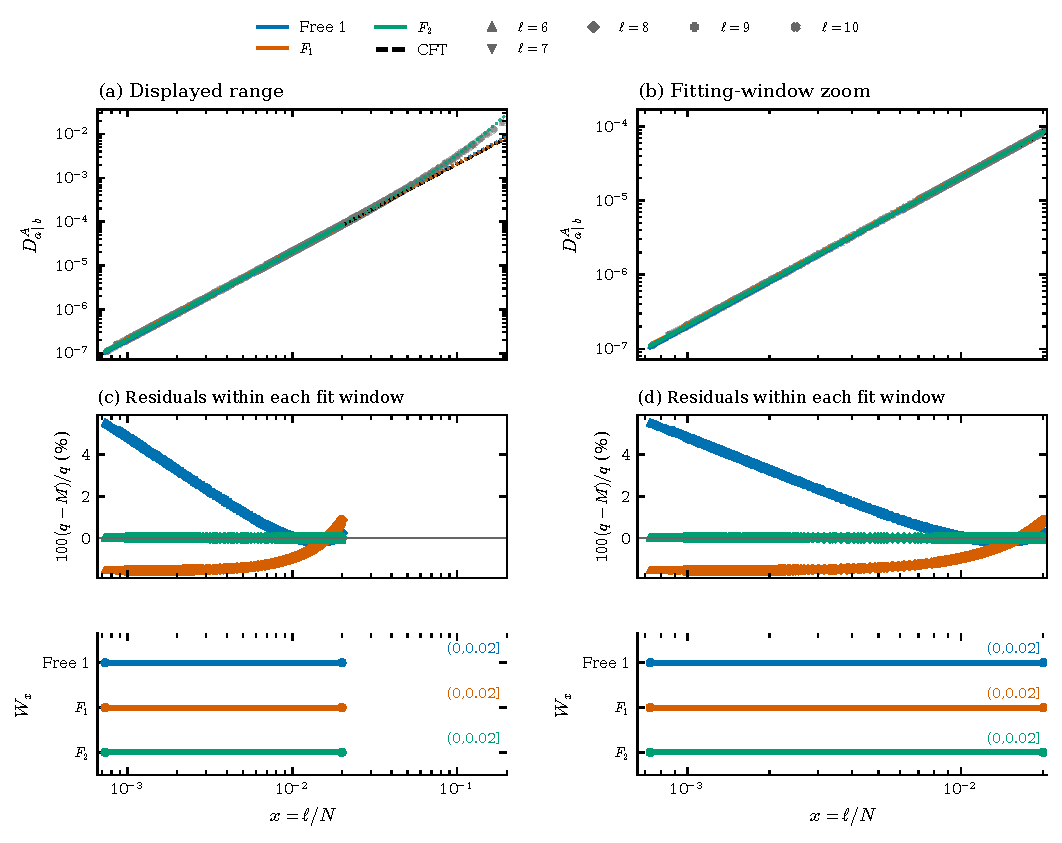
\includegraphics[width=.94\linewidth]{../figs/pair_small_ising_sigma_epsilon.pdf}\par\smallskip
\begingroup\scriptsize\setlength{\tabcolsep}{4pt}
\begin{tabular}{lllrrrrr}\toprule
Set & Model & $W_z$ & $m$ & $c_0$ & $r^{(0)}$ & $c_1$ & $r^{(1)}$\\\midrule
Both & Free 1 & $(0,0.02]$ & 1255 & 0.23069 & 2.0237554 & --- & ---\\
Both & $F_1$ & $(0,0.02]$ & 1255 & 0.2089 & 2 & --- & ---\\
Both & $F_2$ & $(0,0.02]$ & 1255 & 0.20565 & 2 & 12.604 & 4\\
\midrule
Both & CFT & --- & --- & 0.20562 & 2 & --- & ---\\
\bottomrule\end{tabular}
\endgroup
\caption{Ising, small intervals, $\sigma\mid \varepsilon$, at $p=1/2$, $\ell=6,\ldots,10$, and the complete size grid in Eq.~\eqref{eq:extended-grid}. Here $z=x$ and $q=D^A$. Left: all computed data through $z=0.20$; right: a zoom into the common fitting window. Both columns show the same Free 1, $F_1$, and $F_2$ fits. All six directions of this CFT and interval type use the same window. Gray markers denote the data. Colored solid segments lie inside each model\textquotesingle s fitting interval; dotted segments are extrapolations. Black dashed is the supplied CFT series. The observable axes are logarithmic and span the measured data; nonpositive predictions cannot appear there and out-of-range extrapolations leave the panel. Residual ordinates are linear and show $100(q-M)/q$ only on each model\textquotesingle s fitted observations. Bars give the exact fitting intervals. The parameter block follows Eq.~\eqref{eq:fit}, with $c_0,c_1$ multiplying $z^{r^{(0)}},z^{r^{(1)}}$; all coefficients include powers of $\pi$. A dash means an absent fitted term, or no fitting window for CFT. Values shown are rounded; curves use full precision.}
\label{fig:pair-small_ising-sigma-epsilon}
\end{figure}
\begin{figure}[!htbp]\centering
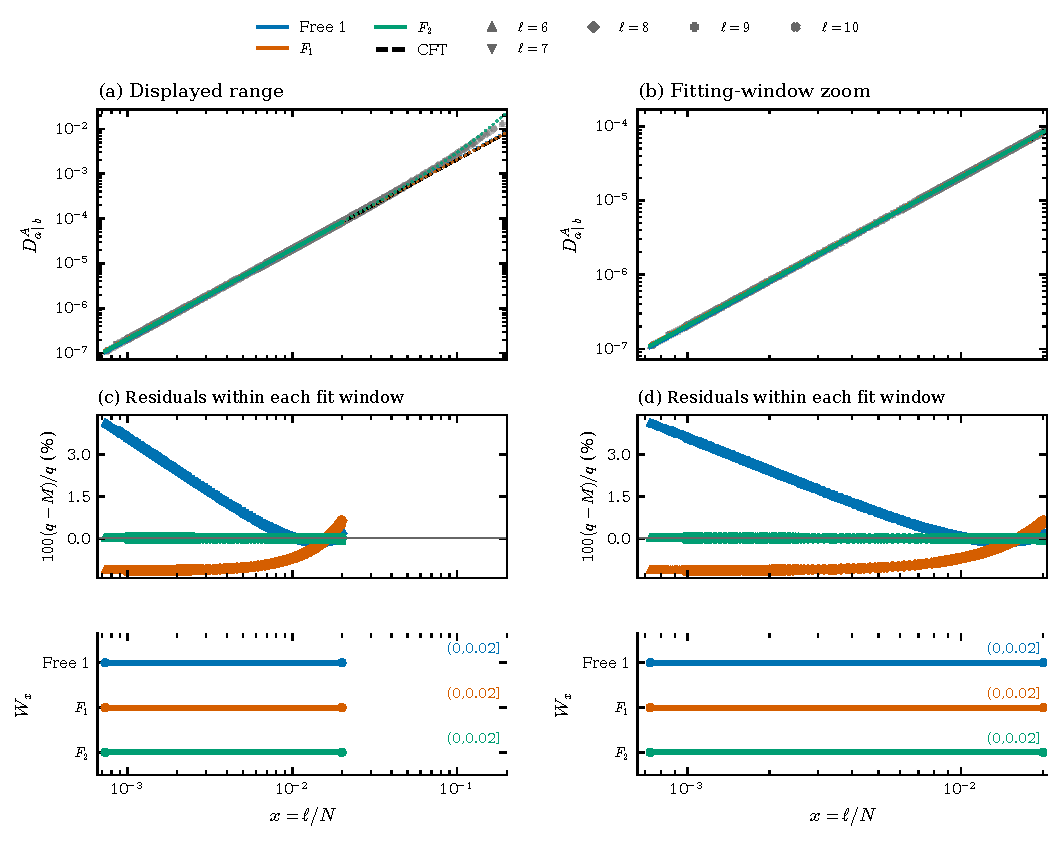
\includegraphics[width=.94\linewidth]{../figs/pair_small_ising_epsilon_sigma.pdf}\par\smallskip
\begingroup\scriptsize\setlength{\tabcolsep}{4pt}
\begin{tabular}{lllrrrrr}\toprule
Set & Model & $W_z$ & $m$ & $c_0$ & $r^{(0)}$ & $c_1$ & $r^{(1)}$\\\midrule
Both & Free 1 & $(0,0.02]$ & 1255 & 0.22393 & 2.0176011 & --- & ---\\
Both & $F_1$ & $(0,0.02]$ & 1255 & 0.20806 & 2 & --- & ---\\
Both & $F_2$ & $(0,0.02]$ & 1255 & 0.20566 & 2 & 9.3133 & 4\\
\midrule
Both & CFT & --- & --- & 0.20562 & 2 & --- & ---\\
\bottomrule\end{tabular}
\endgroup
\caption{Ising, small intervals, $\varepsilon\mid \sigma$, at $p=1/2$, $\ell=6,\ldots,10$, and the complete size grid in Eq.~\eqref{eq:extended-grid}. Here $z=x$ and $q=D^A$. Left: all computed data through $z=0.20$; right: a zoom into the common fitting window. Both columns show the same Free 1, $F_1$, and $F_2$ fits. All six directions of this CFT and interval type use the same window. Gray markers denote the data. Colored solid segments lie inside each model\textquotesingle s fitting interval; dotted segments are extrapolations. Black dashed is the supplied CFT series. The observable axes are logarithmic and span the measured data; nonpositive predictions cannot appear there and out-of-range extrapolations leave the panel. Residual ordinates are linear and show $100(q-M)/q$ only on each model\textquotesingle s fitted observations. Bars give the exact fitting intervals. The parameter block follows Eq.~\eqref{eq:fit}, with $c_0,c_1$ multiplying $z^{r^{(0)}},z^{r^{(1)}}$; all coefficients include powers of $\pi$. A dash means an absent fitted term, or no fitting window for CFT. Values shown are rounded; curves use full precision.}
\label{fig:pair-small_ising-epsilon-sigma}
\end{figure}

\clearpage
\subsection{Compact boson, small intervals}
\label{sec:pair-small_boson}
\begin{figure}[!htbp]\centering
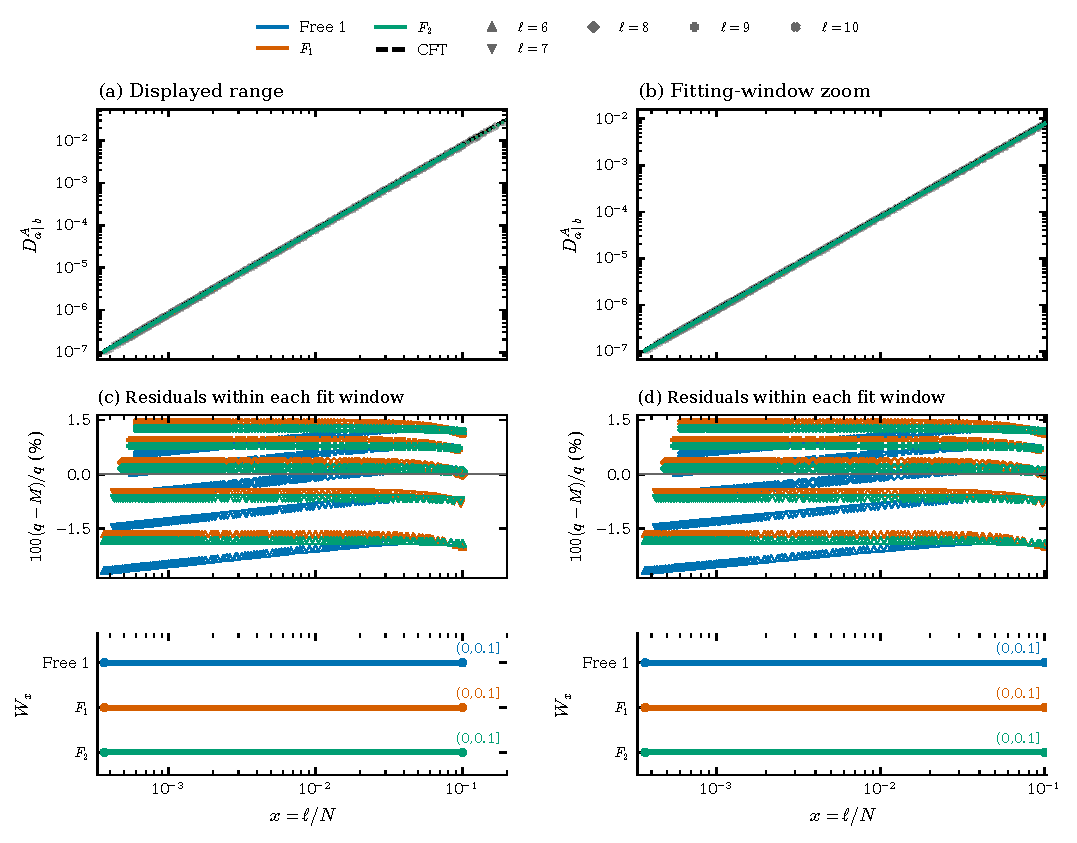
\includegraphics[width=.94\linewidth]{../figs/pair_small_boson_00_ss.pdf}\par\smallskip
\begingroup\scriptsize\setlength{\tabcolsep}{4pt}
\begin{tabular}{lllrrrrr}\toprule
Set & Model & $W_z$ & $m$ & $c_0$ & $r^{(0)}$ & $c_1$ & $r^{(1)}$\\\midrule
Both & Free 1 & $(0,0.1]$ & 598 & 0.77501 & 1.998159 & --- & ---\\
Both & $F_1$ & $(0,0.1]$ & 598 & 0.77866 & 2 & --- & ---\\
Both & $F_2$ & $(0,0.1]$ & 598 & 0.77996 & 2 & -0.1917 & 4\\
\midrule
Both & CFT & --- & --- & 0.82247 & 2 & --- & ---\\
\bottomrule\end{tabular}
\endgroup
\caption{Compact boson, small intervals, $00\mid ss$, at $p=1/2$, $\ell=6,\ldots,10$, and the complete size grid in Eq.~\eqref{eq:extended-grid}. Here $z=x$ and $q=D^A$. Left: all computed data through $z=0.20$; right: a zoom into the common fitting window. Both columns show the same Free 1, $F_1$, and $F_2$ fits. All six directions of this CFT and interval type use the same window. Gray markers denote the data. Colored solid segments lie inside each model\textquotesingle s fitting interval; dotted segments are extrapolations. Black dashed is the supplied CFT series. The observable axes are logarithmic and span the measured data; nonpositive predictions cannot appear there and out-of-range extrapolations leave the panel. Residual ordinates are linear and show $100(q-M)/q$ only on each model\textquotesingle s fitted observations. Bars give the exact fitting intervals. The parameter block follows Eq.~\eqref{eq:fit}, with $c_0,c_1$ multiplying $z^{r^{(0)}},z^{r^{(1)}}$; all coefficients include powers of $\pi$. A dash means an absent fitted term, or no fitting window for CFT. Values shown are rounded; curves use full precision.}
\label{fig:pair-small_boson-00-ss}
\end{figure}
\begin{figure}[!htbp]\centering
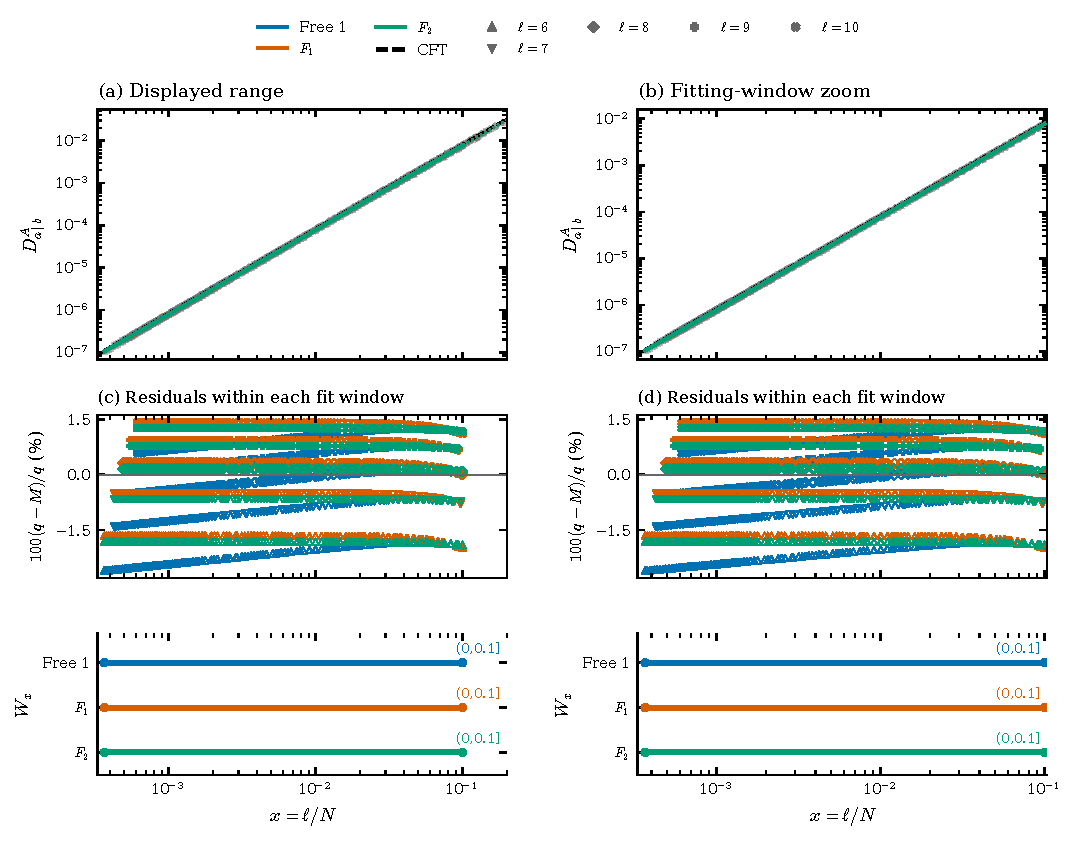
\includegraphics[width=.94\linewidth]{../figs/pair_small_boson_ss_00.pdf}\par\smallskip
\begingroup\scriptsize\setlength{\tabcolsep}{4pt}
\begin{tabular}{lllrrrrr}\toprule
Set & Model & $W_z$ & $m$ & $c_0$ & $r^{(0)}$ & $c_1$ & $r^{(1)}$\\\midrule
Both & Free 1 & $(0,0.1]$ & 598 & 0.77529 & 1.9982698 & --- & ---\\
Both & $F_1$ & $(0,0.1]$ & 598 & 0.77871 & 2 & --- & ---\\
Both & $F_2$ & $(0,0.1]$ & 598 & 0.77995 & 2 & -0.18219 & 4\\
\midrule
Both & CFT & --- & --- & 0.82247 & 2 & --- & ---\\
\bottomrule\end{tabular}
\endgroup
\caption{Compact boson, small intervals, $ss\mid 00$, at $p=1/2$, $\ell=6,\ldots,10$, and the complete size grid in Eq.~\eqref{eq:extended-grid}. Here $z=x$ and $q=D^A$. Left: all computed data through $z=0.20$; right: a zoom into the common fitting window. Both columns show the same Free 1, $F_1$, and $F_2$ fits. All six directions of this CFT and interval type use the same window. Gray markers denote the data. Colored solid segments lie inside each model\textquotesingle s fitting interval; dotted segments are extrapolations. Black dashed is the supplied CFT series. The observable axes are logarithmic and span the measured data; nonpositive predictions cannot appear there and out-of-range extrapolations leave the panel. Residual ordinates are linear and show $100(q-M)/q$ only on each model\textquotesingle s fitted observations. Bars give the exact fitting intervals. The parameter block follows Eq.~\eqref{eq:fit}, with $c_0,c_1$ multiplying $z^{r^{(0)}},z^{r^{(1)}}$; all coefficients include powers of $\pi$. A dash means an absent fitted term, or no fitting window for CFT. Values shown are rounded; curves use full precision.}
\label{fig:pair-small_boson-ss-00}
\end{figure}
\begin{figure}[!htbp]\centering
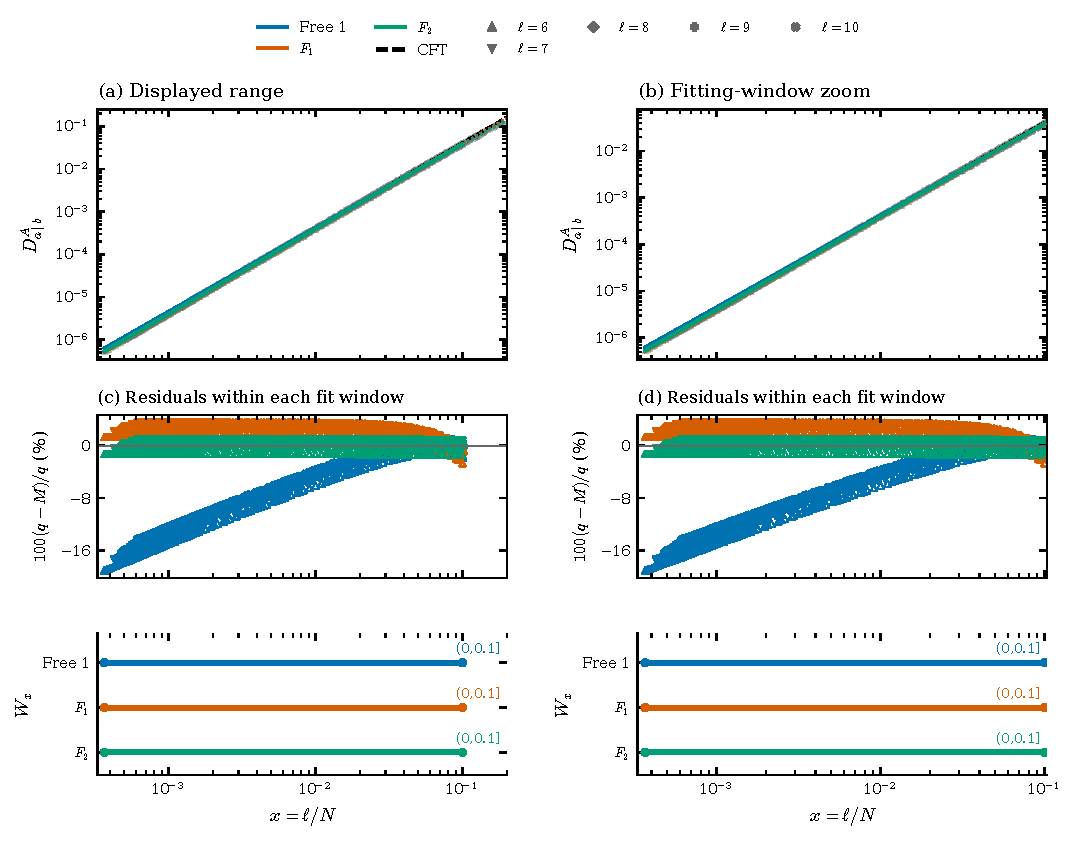
\includegraphics[width=.94\linewidth]{../figs/pair_small_boson_00_3s_s.pdf}\par\smallskip
\begingroup\scriptsize\setlength{\tabcolsep}{4pt}
\begin{tabular}{lllrrrrr}\toprule
Set & Model & $W_z$ & $m$ & $c_0$ & $r^{(0)}$ & $c_1$ & $r^{(1)}$\\\midrule
Both & Free 1 & $(0,0.1]$ & 598 & 3.5315 & 1.9648776 & --- & ---\\
Both & $F_1$ & $(0,0.1]$ & 598 & 3.8623 & 2 & --- & ---\\
Both & $F_2$ & $(0,0.1]$ & 598 & 3.964 & 2 & -15.02 & 4\\
\midrule
Both & CFT & --- & --- & 4.1123 & 2 & --- & ---\\
\bottomrule\end{tabular}
\endgroup
\caption{Compact boson, small intervals, $00\mid 3s,s$, at $p=1/2$, $\ell=6,\ldots,10$, and the complete size grid in Eq.~\eqref{eq:extended-grid}. Here $z=x$ and $q=D^A$. Left: all computed data through $z=0.20$; right: a zoom into the common fitting window. Both columns show the same Free 1, $F_1$, and $F_2$ fits. All six directions of this CFT and interval type use the same window. Gray markers denote the data. Colored solid segments lie inside each model\textquotesingle s fitting interval; dotted segments are extrapolations. Black dashed is the supplied CFT series. The observable axes are logarithmic and span the measured data; nonpositive predictions cannot appear there and out-of-range extrapolations leave the panel. Residual ordinates are linear and show $100(q-M)/q$ only on each model\textquotesingle s fitted observations. Bars give the exact fitting intervals. The parameter block follows Eq.~\eqref{eq:fit}, with $c_0,c_1$ multiplying $z^{r^{(0)}},z^{r^{(1)}}$; all coefficients include powers of $\pi$. A dash means an absent fitted term, or no fitting window for CFT. Values shown are rounded; curves use full precision.}
\label{fig:pair-small_boson-00-3s_s}
\end{figure}
\begin{figure}[!htbp]\centering
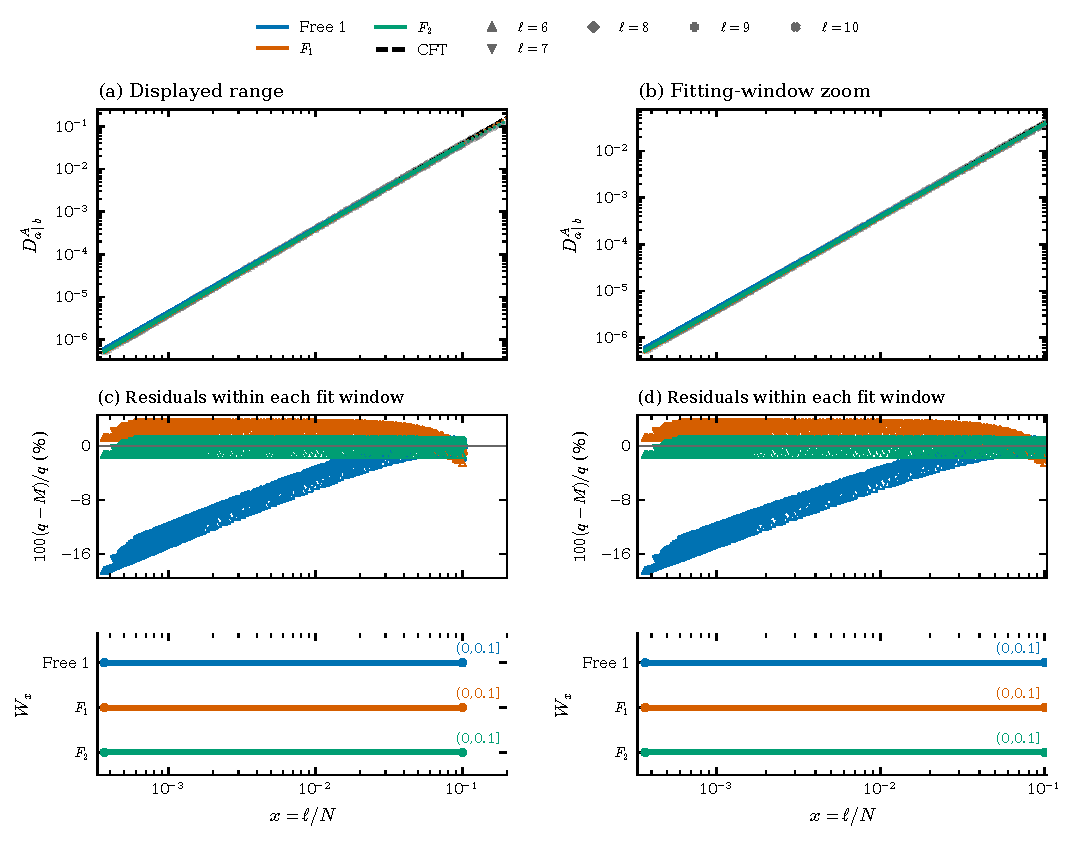
\includegraphics[width=.94\linewidth]{../figs/pair_small_boson_3s_s_00.pdf}\par\smallskip
\begingroup\scriptsize\setlength{\tabcolsep}{4pt}
\begin{tabular}{lllrrrrr}\toprule
Set & Model & $W_z$ & $m$ & $c_0$ & $r^{(0)}$ & $c_1$ & $r^{(1)}$\\\midrule
Both & Free 1 & $(0,0.1]$ & 598 & 3.545 & 1.9660249 & --- & ---\\
Both & $F_1$ & $(0,0.1]$ & 598 & 3.8657 & 2 & --- & ---\\
Both & $F_2$ & $(0,0.1]$ & 598 & 3.9643 & 2 & -14.541 & 4\\
\midrule
Both & CFT & --- & --- & 4.1123 & 2 & --- & ---\\
\bottomrule\end{tabular}
\endgroup
\caption{Compact boson, small intervals, $3s,s\mid 00$, at $p=1/2$, $\ell=6,\ldots,10$, and the complete size grid in Eq.~\eqref{eq:extended-grid}. Here $z=x$ and $q=D^A$. Left: all computed data through $z=0.20$; right: a zoom into the common fitting window. Both columns show the same Free 1, $F_1$, and $F_2$ fits. All six directions of this CFT and interval type use the same window. Gray markers denote the data. Colored solid segments lie inside each model\textquotesingle s fitting interval; dotted segments are extrapolations. Black dashed is the supplied CFT series. The observable axes are logarithmic and span the measured data; nonpositive predictions cannot appear there and out-of-range extrapolations leave the panel. Residual ordinates are linear and show $100(q-M)/q$ only on each model\textquotesingle s fitted observations. Bars give the exact fitting intervals. The parameter block follows Eq.~\eqref{eq:fit}, with $c_0,c_1$ multiplying $z^{r^{(0)}},z^{r^{(1)}}$; all coefficients include powers of $\pi$. A dash means an absent fitted term, or no fitting window for CFT. Values shown are rounded; curves use full precision.}
\label{fig:pair-small_boson-3s_s-00}
\end{figure}
\begin{figure}[!htbp]\centering
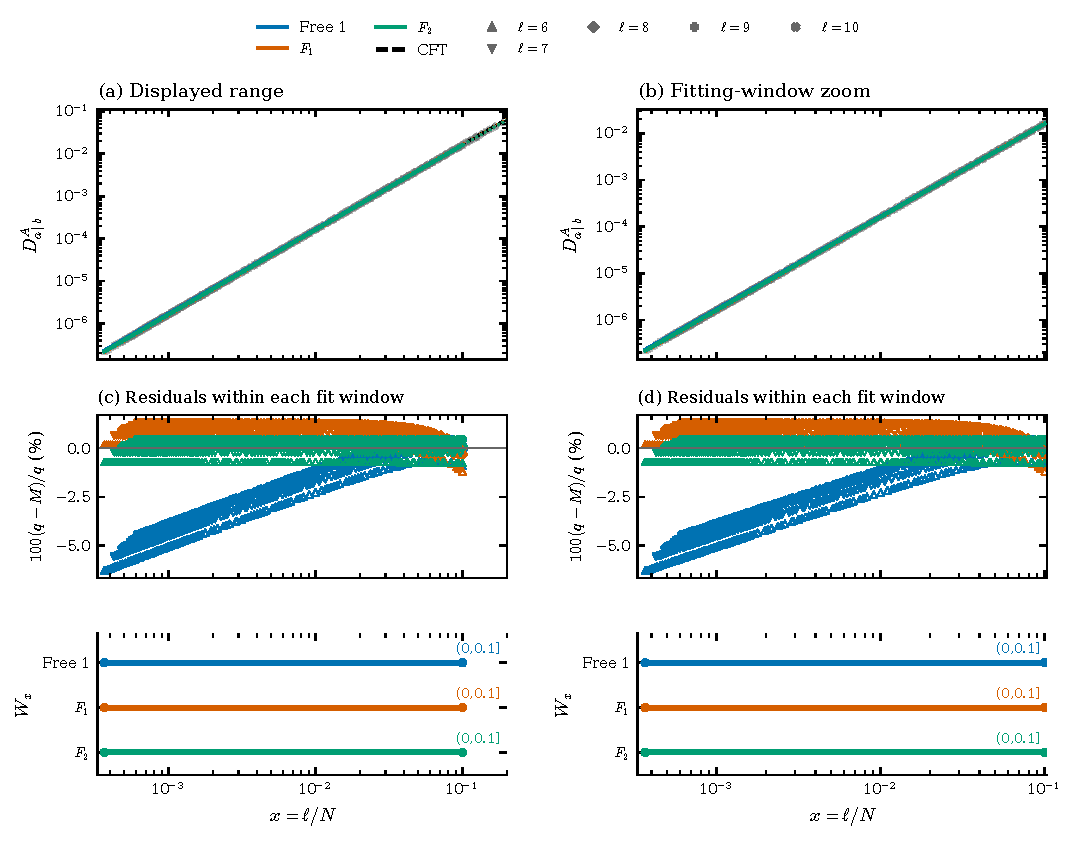
\includegraphics[width=.94\linewidth]{../figs/pair_small_boson_ss_3s_s.pdf}\par\smallskip
\begingroup\scriptsize\setlength{\tabcolsep}{4pt}
\begin{tabular}{lllrrrrr}\toprule
Set & Model & $W_z$ & $m$ & $c_0$ & $r^{(0)}$ & $c_1$ & $r^{(1)}$\\\midrule
Both & Free 1 & $(0,0.1]$ & 598 & 1.5661 & 1.9883068 & --- & ---\\
Both & $F_1$ & $(0,0.1]$ & 598 & 1.6134 & 2 & --- & ---\\
Both & $F_2$ & $(0,0.1]$ & 598 & 1.6276 & 2 & -2.0896 & 4\\
\midrule
Both & CFT & --- & --- & 1.6449 & 2 & --- & ---\\
\bottomrule\end{tabular}
\endgroup
\caption{Compact boson, small intervals, $ss\mid 3s,s$, at $p=1/2$, $\ell=6,\ldots,10$, and the complete size grid in Eq.~\eqref{eq:extended-grid}. Here $z=x$ and $q=D^A$. Left: all computed data through $z=0.20$; right: a zoom into the common fitting window. Both columns show the same Free 1, $F_1$, and $F_2$ fits. All six directions of this CFT and interval type use the same window. Gray markers denote the data. Colored solid segments lie inside each model\textquotesingle s fitting interval; dotted segments are extrapolations. Black dashed is the supplied CFT series. The observable axes are logarithmic and span the measured data; nonpositive predictions cannot appear there and out-of-range extrapolations leave the panel. Residual ordinates are linear and show $100(q-M)/q$ only on each model\textquotesingle s fitted observations. Bars give the exact fitting intervals. The parameter block follows Eq.~\eqref{eq:fit}, with $c_0,c_1$ multiplying $z^{r^{(0)}},z^{r^{(1)}}$; all coefficients include powers of $\pi$. A dash means an absent fitted term, or no fitting window for CFT. Values shown are rounded; curves use full precision.}
\label{fig:pair-small_boson-ss-3s_s}
\end{figure}
\begin{figure}[!htbp]\centering
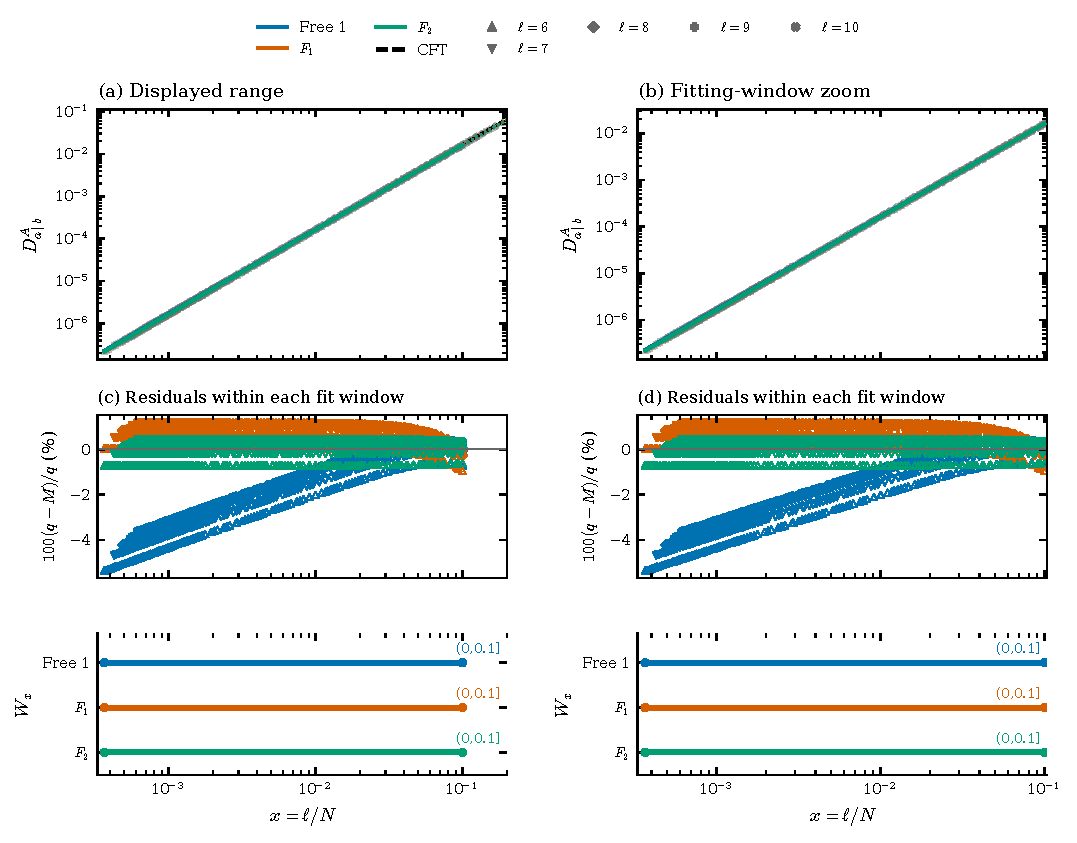
\includegraphics[width=.94\linewidth]{../figs/pair_small_boson_3s_s_ss.pdf}\par\smallskip
\begingroup\scriptsize\setlength{\tabcolsep}{4pt}
\begin{tabular}{lllrrrrr}\toprule
Set & Model & $W_z$ & $m$ & $c_0$ & $r^{(0)}$ & $c_1$ & $r^{(1)}$\\\midrule
Both & Free 1 & $(0,0.1]$ & 598 & 1.576 & 1.9902202 & --- & ---\\
Both & $F_1$ & $(0,0.1]$ & 598 & 1.6157 & 2 & --- & ---\\
Both & $F_2$ & $(0,0.1]$ & 598 & 1.6276 & 2 & -1.7507 & 4\\
\midrule
Both & CFT & --- & --- & 1.6449 & 2 & --- & ---\\
\bottomrule\end{tabular}
\endgroup
\caption{Compact boson, small intervals, $3s,s\mid ss$, at $p=1/2$, $\ell=6,\ldots,10$, and the complete size grid in Eq.~\eqref{eq:extended-grid}. Here $z=x$ and $q=D^A$. Left: all computed data through $z=0.20$; right: a zoom into the common fitting window. Both columns show the same Free 1, $F_1$, and $F_2$ fits. All six directions of this CFT and interval type use the same window. Gray markers denote the data. Colored solid segments lie inside each model\textquotesingle s fitting interval; dotted segments are extrapolations. Black dashed is the supplied CFT series. The observable axes are logarithmic and span the measured data; nonpositive predictions cannot appear there and out-of-range extrapolations leave the panel. Residual ordinates are linear and show $100(q-M)/q$ only on each model\textquotesingle s fitted observations. Bars give the exact fitting intervals. The parameter block follows Eq.~\eqref{eq:fit}, with $c_0,c_1$ multiplying $z^{r^{(0)}},z^{r^{(1)}}$; all coefficients include powers of $\pi$. A dash means an absent fitted term, or no fitting window for CFT. Values shown are rounded; curves use full precision.}
\label{fig:pair-small_boson-3s_s-ss}
\end{figure}

\clearpage
\subsection{Ising, large intervals}
\label{sec:pair-large_ising}
\begin{figure}[!htbp]\centering
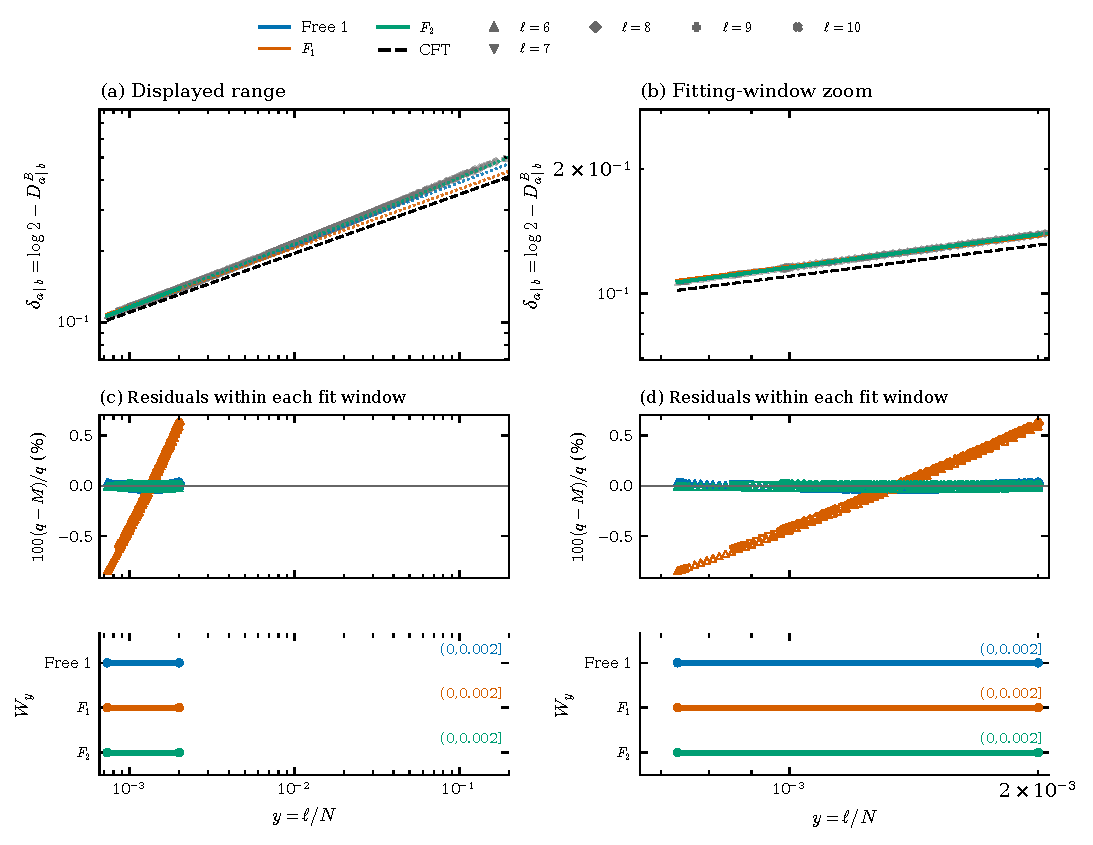
\includegraphics[width=.94\linewidth]{../figs/pair_large_ising_I_sigma.pdf}\par\smallskip
\begingroup\scriptsize\setlength{\tabcolsep}{4pt}
\begin{tabular}{lllrrrrr}\toprule
Set & Model & $W_z$ & $m$ & $c_0$ & $r^{(0)}$ & $c_1$ & $r^{(1)}$\\\midrule
Both & Free 1 & $(0,0.002]$ & 260 & 0.71994 & 0.2646516 & --- & ---\\
Both & $F_1$ & $(0,0.002]$ & 260 & 0.65339 & 0.25 & --- & ---\\
Both & $F_2$ & $(0,0.002]$ & 260 & 0.61463 & 0.25 & 0.20243 & 0.5\\
\midrule
Both & CFT & --- & --- & 0.61965 & 0.25 & --- & ---\\
\bottomrule\end{tabular}
\endgroup
\caption{Ising, large intervals, $I\mid \sigma$, at $p=1/2$, $\ell=6,\ldots,10$, and the complete size grid in Eq.~\eqref{eq:extended-grid}. Here $z=y$ and $q=\delta=\log2-D^B$. Left: all computed data through $z=0.20$; right: a zoom into the common fitting window. Both columns show the same Free 1, $F_1$, and $F_2$ fits. All six directions of this CFT and interval type use the same window. Gray markers denote the data. Colored solid segments lie inside each model\textquotesingle s fitting interval; dotted segments are extrapolations. Black dashed is the analytical CFT leading deficit. The observable axes are logarithmic and span the measured data; nonpositive predictions cannot appear there and out-of-range extrapolations leave the panel. Residual ordinates are linear and show $100(q-M)/q$ only on each model\textquotesingle s fitted observations. Bars give the exact fitting intervals. The parameter block follows Eq.~\eqref{eq:fit}, with $c_0,c_1$ multiplying $z^{r^{(0)}},z^{r^{(1)}}$; all coefficients include powers of $\pi$. A dash means an absent fitted term, or no fitting window for CFT. Values shown are rounded; curves use full precision.}
\label{fig:pair-large_ising-I-sigma}
\end{figure}
\begin{figure}[!htbp]\centering
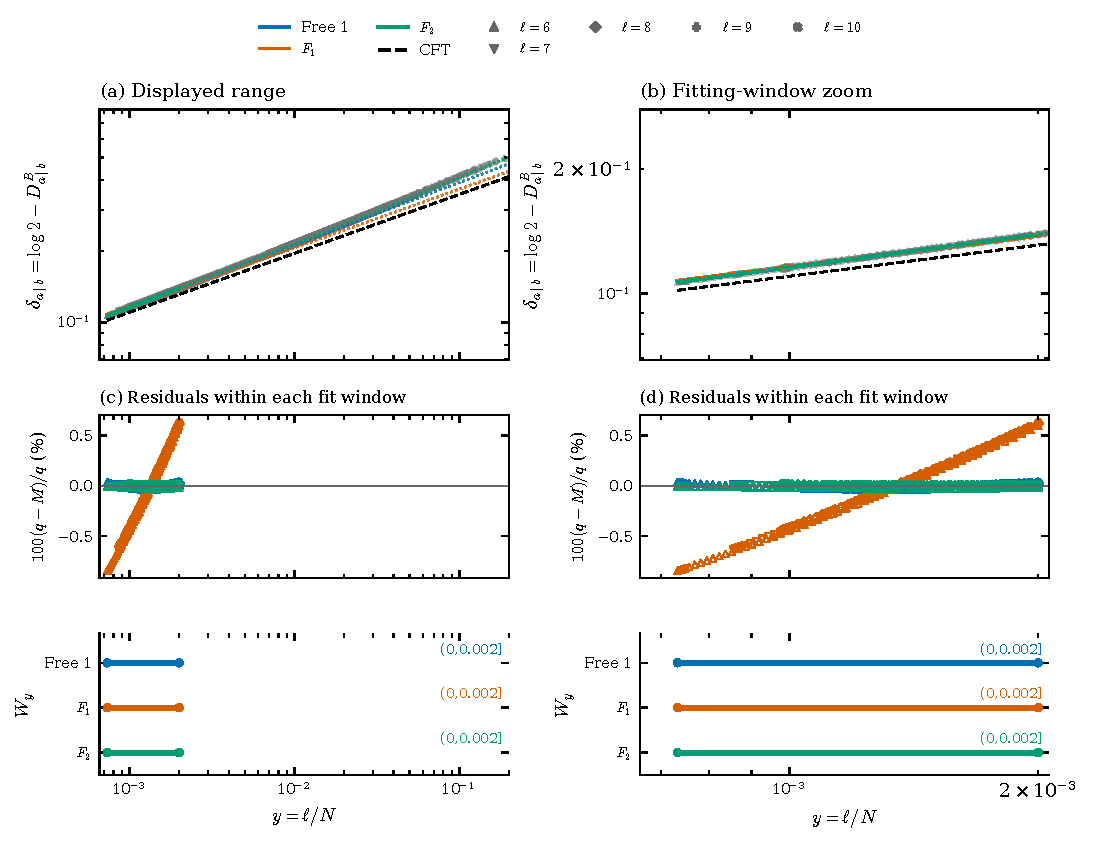
\includegraphics[width=.94\linewidth]{../figs/pair_large_ising_sigma_I.pdf}\par\smallskip
\begingroup\scriptsize\setlength{\tabcolsep}{4pt}
\begin{tabular}{lllrrrrr}\toprule
Set & Model & $W_z$ & $m$ & $c_0$ & $r^{(0)}$ & $c_1$ & $r^{(1)}$\\\midrule
Both & Free 1 & $(0,0.002]$ & 260 & 0.71995 & 0.2646531 & --- & ---\\
Both & $F_1$ & $(0,0.002]$ & 260 & 0.65339 & 0.25 & --- & ---\\
Both & $F_2$ & $(0,0.002]$ & 260 & 0.61462 & 0.25 & 0.20245 & 0.5\\
\midrule
Both & CFT & --- & --- & 0.61965 & 0.25 & --- & ---\\
\bottomrule\end{tabular}
\endgroup
\caption{Ising, large intervals, $\sigma\mid I$, at $p=1/2$, $\ell=6,\ldots,10$, and the complete size grid in Eq.~\eqref{eq:extended-grid}. Here $z=y$ and $q=\delta=\log2-D^B$. Left: all computed data through $z=0.20$; right: a zoom into the common fitting window. Both columns show the same Free 1, $F_1$, and $F_2$ fits. All six directions of this CFT and interval type use the same window. Gray markers denote the data. Colored solid segments lie inside each model\textquotesingle s fitting interval; dotted segments are extrapolations. Black dashed is the analytical CFT leading deficit. The observable axes are logarithmic and span the measured data; nonpositive predictions cannot appear there and out-of-range extrapolations leave the panel. Residual ordinates are linear and show $100(q-M)/q$ only on each model\textquotesingle s fitted observations. Bars give the exact fitting intervals. The parameter block follows Eq.~\eqref{eq:fit}, with $c_0,c_1$ multiplying $z^{r^{(0)}},z^{r^{(1)}}$; all coefficients include powers of $\pi$. A dash means an absent fitted term, or no fitting window for CFT. Values shown are rounded; curves use full precision.}
\label{fig:pair-large_ising-sigma-I}
\end{figure}
\begin{figure}[!htbp]\centering
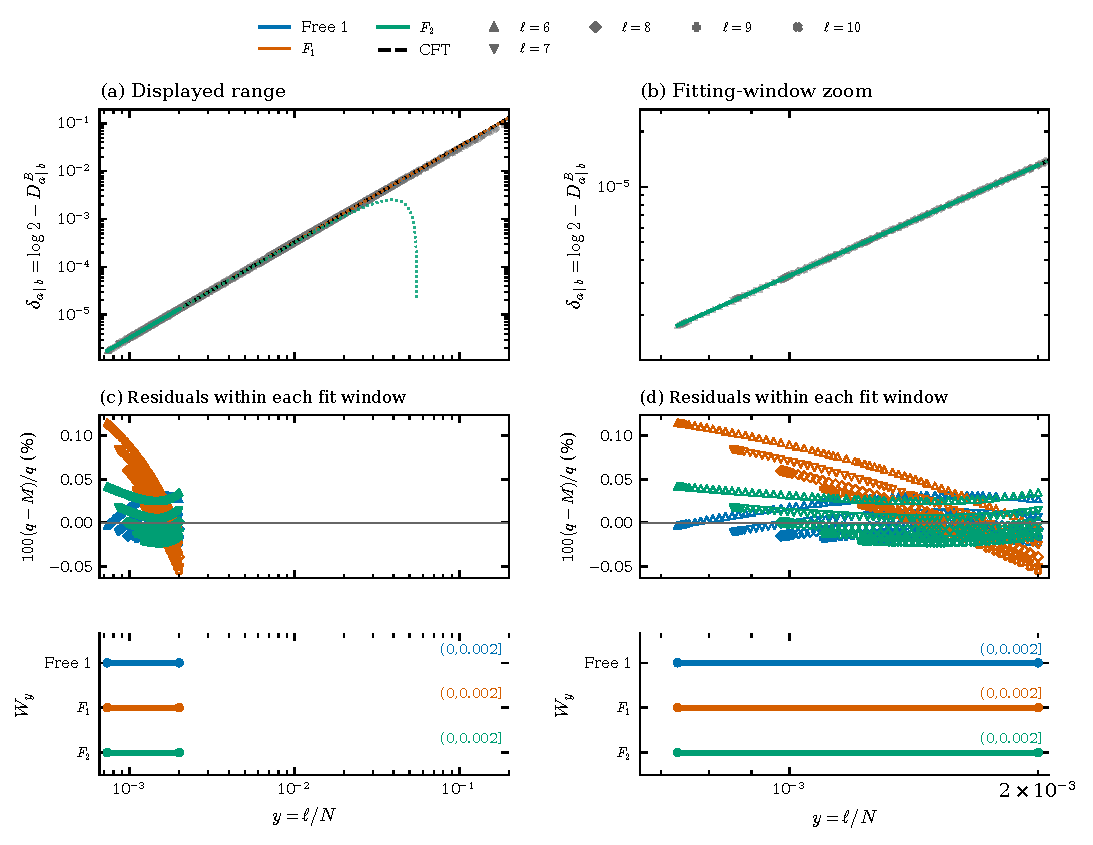
\includegraphics[width=.94\linewidth]{../figs/pair_large_ising_I_epsilon.pdf}\par\smallskip
\begingroup\scriptsize\setlength{\tabcolsep}{4pt}
\begin{tabular}{lllrrrrr}\toprule
Set & Model & $W_z$ & $m$ & $c_0$ & $r^{(0)}$ & $c_1$ & $r^{(1)}$\\\midrule
Both & Free 1 & $(0,0.002]$ & 260 & 3.2548 & 1.9985103 & --- & ---\\
Both & $F_1$ & $(0,0.002]$ & 260 & 3.2861 & 2 & --- & ---\\
Both & $F_2$ & $(0,0.002]$ & 260 & 3.289 & 2 & -1070.2 & 4\\
\midrule
Both & CFT & --- & --- & 3.2899 & 2 & --- & ---\\
\bottomrule\end{tabular}
\endgroup
\caption{Ising, large intervals, $I\mid \varepsilon$, at $p=1/2$, $\ell=6,\ldots,10$, and the complete size grid in Eq.~\eqref{eq:extended-grid}. Here $z=y$ and $q=\delta=\log2-D^B$. Left: all computed data through $z=0.20$; right: a zoom into the common fitting window. Both columns show the same Free 1, $F_1$, and $F_2$ fits. All six directions of this CFT and interval type use the same window. Gray markers denote the data. Colored solid segments lie inside each model\textquotesingle s fitting interval; dotted segments are extrapolations. Black dashed is the analytical CFT leading deficit. The observable axes are logarithmic and span the measured data; nonpositive predictions cannot appear there and out-of-range extrapolations leave the panel. Residual ordinates are linear and show $100(q-M)/q$ only on each model\textquotesingle s fitted observations. Bars give the exact fitting intervals. The parameter block follows Eq.~\eqref{eq:fit}, with $c_0,c_1$ multiplying $z^{r^{(0)}},z^{r^{(1)}}$; all coefficients include powers of $\pi$. A dash means an absent fitted term, or no fitting window for CFT. Values shown are rounded; curves use full precision.}
\label{fig:pair-large_ising-I-epsilon}
\end{figure}
\begin{figure}[!htbp]\centering
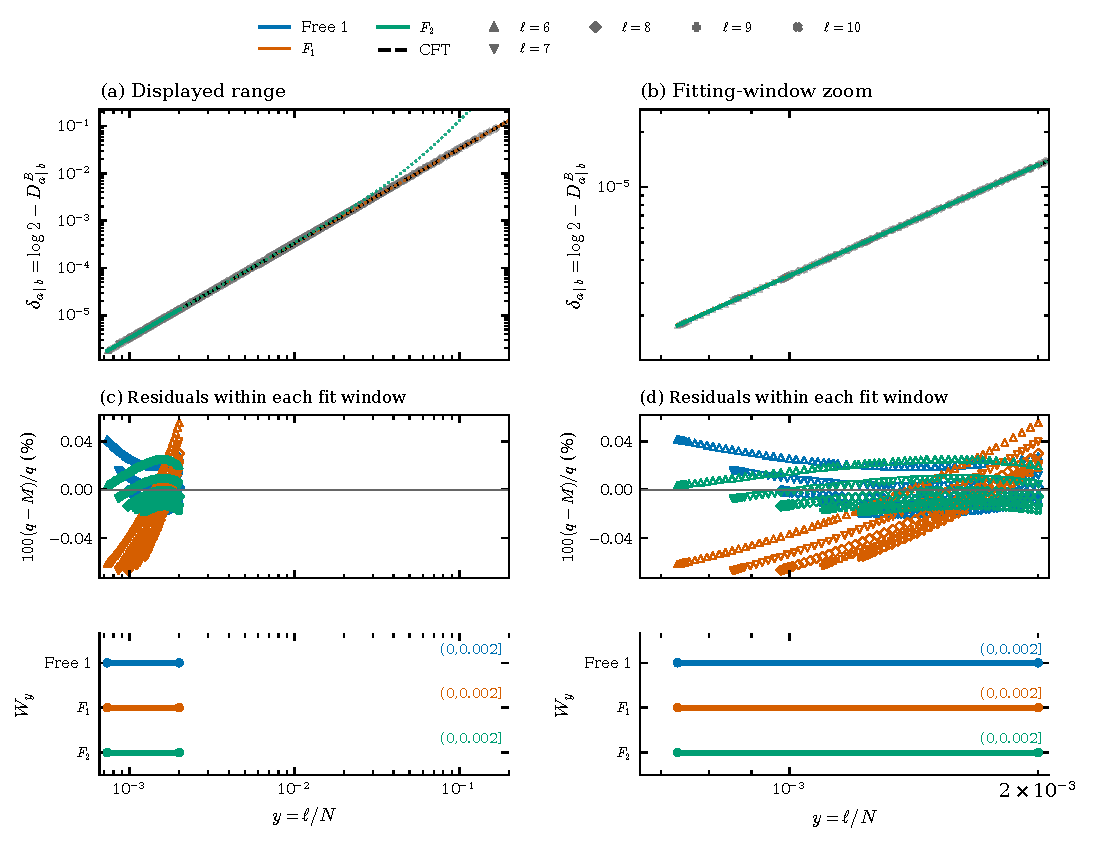
\includegraphics[width=.94\linewidth]{../figs/pair_large_ising_epsilon_I.pdf}\par\smallskip
\begingroup\scriptsize\setlength{\tabcolsep}{4pt}
\begin{tabular}{lllrrrrr}\toprule
Set & Model & $W_z$ & $m$ & $c_0$ & $r^{(0)}$ & $c_1$ & $r^{(1)}$\\\midrule
Both & Free 1 & $(0,0.002]$ & 260 & 3.3242 & 2.0013063 & --- & ---\\
Both & $F_1$ & $(0,0.002]$ & 260 & 3.2964 & 2 & --- & ---\\
Both & $F_2$ & $(0,0.002]$ & 260 & 3.2938 & 2 & 959.21 & 4\\
\midrule
Both & CFT & --- & --- & 3.2899 & 2 & --- & ---\\
\bottomrule\end{tabular}
\endgroup
\caption{Ising, large intervals, $\varepsilon\mid I$, at $p=1/2$, $\ell=6,\ldots,10$, and the complete size grid in Eq.~\eqref{eq:extended-grid}. Here $z=y$ and $q=\delta=\log2-D^B$. Left: all computed data through $z=0.20$; right: a zoom into the common fitting window. Both columns show the same Free 1, $F_1$, and $F_2$ fits. All six directions of this CFT and interval type use the same window. Gray markers denote the data. Colored solid segments lie inside each model\textquotesingle s fitting interval; dotted segments are extrapolations. Black dashed is the analytical CFT leading deficit. The observable axes are logarithmic and span the measured data; nonpositive predictions cannot appear there and out-of-range extrapolations leave the panel. Residual ordinates are linear and show $100(q-M)/q$ only on each model\textquotesingle s fitted observations. Bars give the exact fitting intervals. The parameter block follows Eq.~\eqref{eq:fit}, with $c_0,c_1$ multiplying $z^{r^{(0)}},z^{r^{(1)}}$; all coefficients include powers of $\pi$. A dash means an absent fitted term, or no fitting window for CFT. Values shown are rounded; curves use full precision.}
\label{fig:pair-large_ising-epsilon-I}
\end{figure}
\begin{figure}[!htbp]\centering
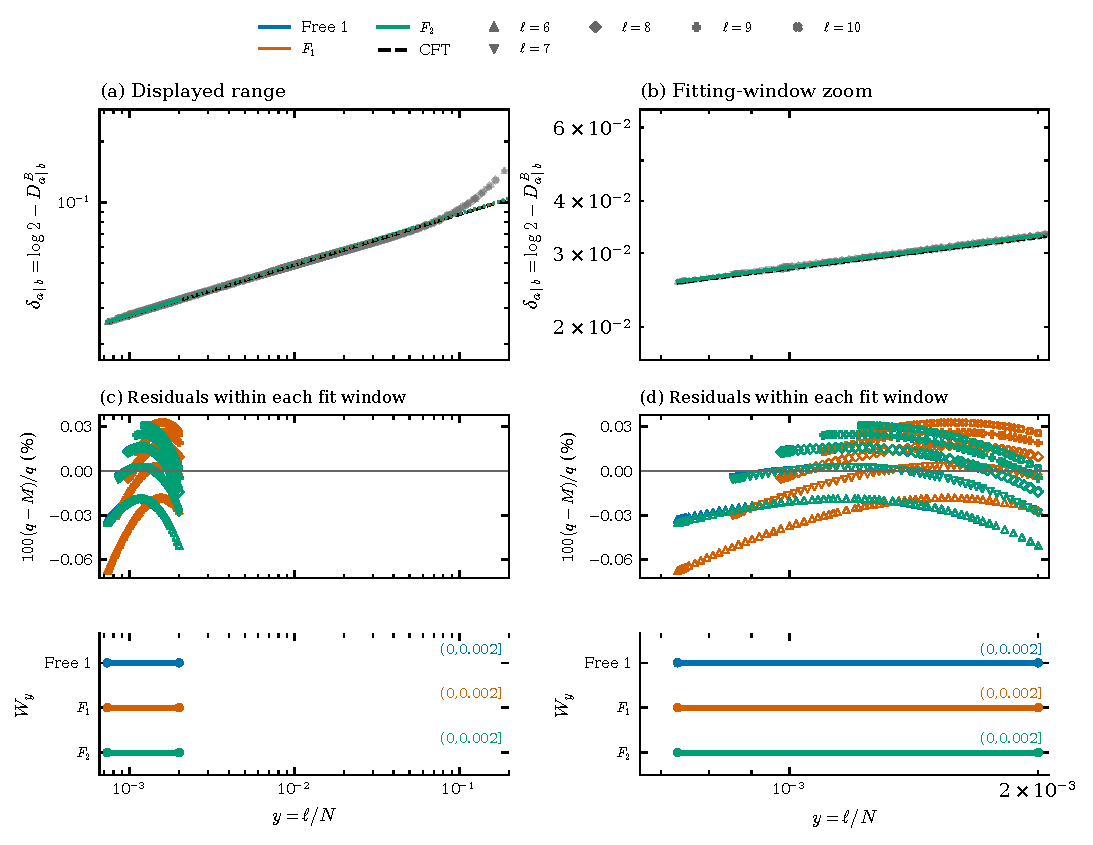
\includegraphics[width=.94\linewidth]{../figs/pair_large_ising_sigma_epsilon.pdf}\par\smallskip
\begingroup\scriptsize\setlength{\tabcolsep}{4pt}
\begin{tabular}{lllrrrrr}\toprule
Set & Model & $W_z$ & $m$ & $c_0$ & $r^{(0)}$ & $c_1$ & $r^{(1)}$\\\midrule
Both & Free 1 & $(0,0.002]$ & 260 & 0.15691 & 0.2505807 & --- & ---\\
Both & $F_1$ & $(0,0.002]$ & 260 & 0.15631 & 0.25 & --- & ---\\
Both & $F_2$ & $(0,0.002]$ & 260 & 0.15595 & 0.25 & 0.0018716 & 0.5\\
\midrule
Both & CFT & --- & --- & 0.15491 & 0.25 & --- & ---\\
\bottomrule\end{tabular}
\endgroup
\caption{Ising, large intervals, $\sigma\mid \varepsilon$, at $p=1/2$, $\ell=6,\ldots,10$, and the complete size grid in Eq.~\eqref{eq:extended-grid}. Here $z=y$ and $q=\delta=\log2-D^B$. Left: all computed data through $z=0.20$; right: a zoom into the common fitting window. Both columns show the same Free 1, $F_1$, and $F_2$ fits. All six directions of this CFT and interval type use the same window. Gray markers denote the data. Colored solid segments lie inside each model\textquotesingle s fitting interval; dotted segments are extrapolations. Black dashed is the analytical CFT leading deficit. The observable axes are logarithmic and span the measured data; nonpositive predictions cannot appear there and out-of-range extrapolations leave the panel. Residual ordinates are linear and show $100(q-M)/q$ only on each model\textquotesingle s fitted observations. Bars give the exact fitting intervals. The parameter block follows Eq.~\eqref{eq:fit}, with $c_0,c_1$ multiplying $z^{r^{(0)}},z^{r^{(1)}}$; all coefficients include powers of $\pi$. A dash means an absent fitted term, or no fitting window for CFT. Values shown are rounded; curves use full precision.}
\label{fig:pair-large_ising-sigma-epsilon}
\end{figure}
\begin{figure}[!htbp]\centering
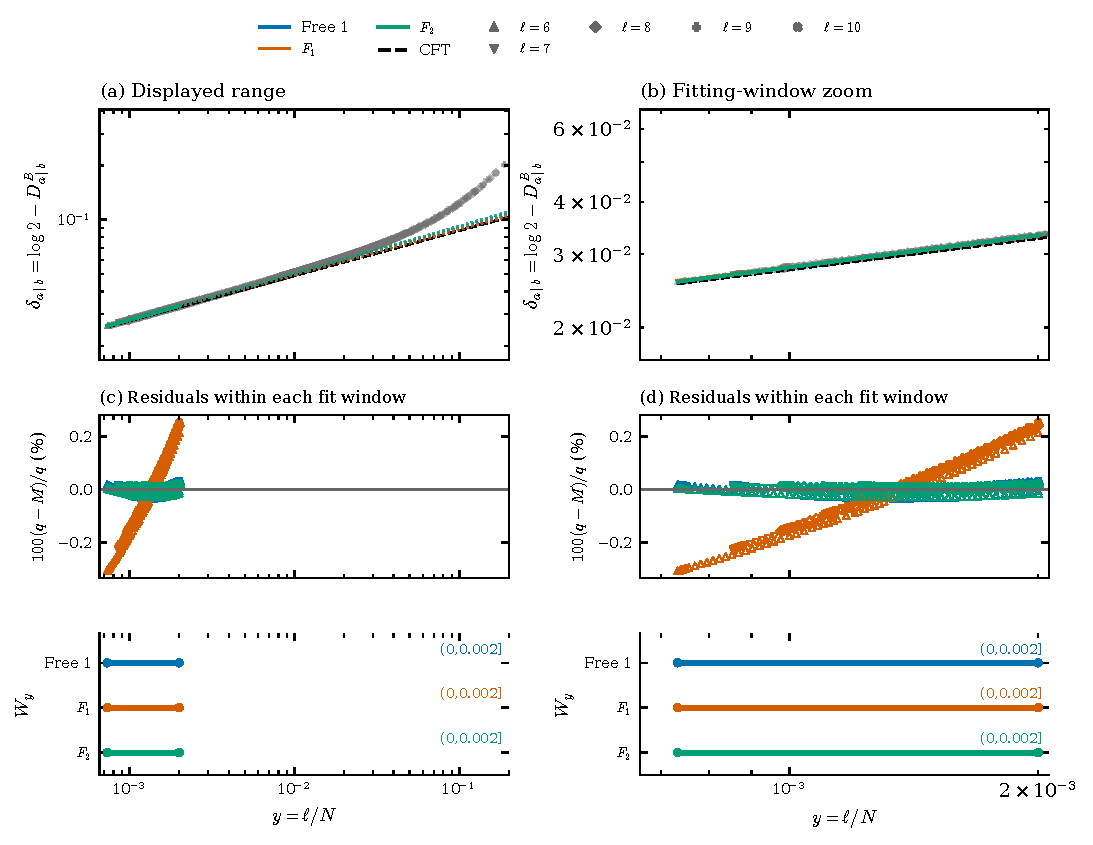
\includegraphics[width=.94\linewidth]{../figs/pair_large_ising_epsilon_sigma.pdf}\par\smallskip
\begingroup\scriptsize\setlength{\tabcolsep}{4pt}
\begin{tabular}{lllrrrrr}\toprule
Set & Model & $W_z$ & $m$ & $c_0$ & $r^{(0)}$ & $c_1$ & $r^{(1)}$\\\midrule
Both & Free 1 & $(0,0.002]$ & 260 & 0.16288 & 0.2554384 & --- & ---\\
Both & $F_1$ & $(0,0.002]$ & 260 & 0.15712 & 0.25 & --- & ---\\
Both & $F_2$ & $(0,0.002]$ & 260 & 0.15365 & 0.25 & 0.018087 & 0.5\\
\midrule
Both & CFT & --- & --- & 0.15491 & 0.25 & --- & ---\\
\bottomrule\end{tabular}
\endgroup
\caption{Ising, large intervals, $\varepsilon\mid \sigma$, at $p=1/2$, $\ell=6,\ldots,10$, and the complete size grid in Eq.~\eqref{eq:extended-grid}. Here $z=y$ and $q=\delta=\log2-D^B$. Left: all computed data through $z=0.20$; right: a zoom into the common fitting window. Both columns show the same Free 1, $F_1$, and $F_2$ fits. All six directions of this CFT and interval type use the same window. Gray markers denote the data. Colored solid segments lie inside each model\textquotesingle s fitting interval; dotted segments are extrapolations. Black dashed is the analytical CFT leading deficit. The observable axes are logarithmic and span the measured data; nonpositive predictions cannot appear there and out-of-range extrapolations leave the panel. Residual ordinates are linear and show $100(q-M)/q$ only on each model\textquotesingle s fitted observations. Bars give the exact fitting intervals. The parameter block follows Eq.~\eqref{eq:fit}, with $c_0,c_1$ multiplying $z^{r^{(0)}},z^{r^{(1)}}$; all coefficients include powers of $\pi$. A dash means an absent fitted term, or no fitting window for CFT. Values shown are rounded; curves use full precision.}
\label{fig:pair-large_ising-epsilon-sigma}
\end{figure}

\clearpage
\subsection{Compact boson, large intervals}
\label{sec:pair-large_boson}
\begin{figure}[!htbp]\centering
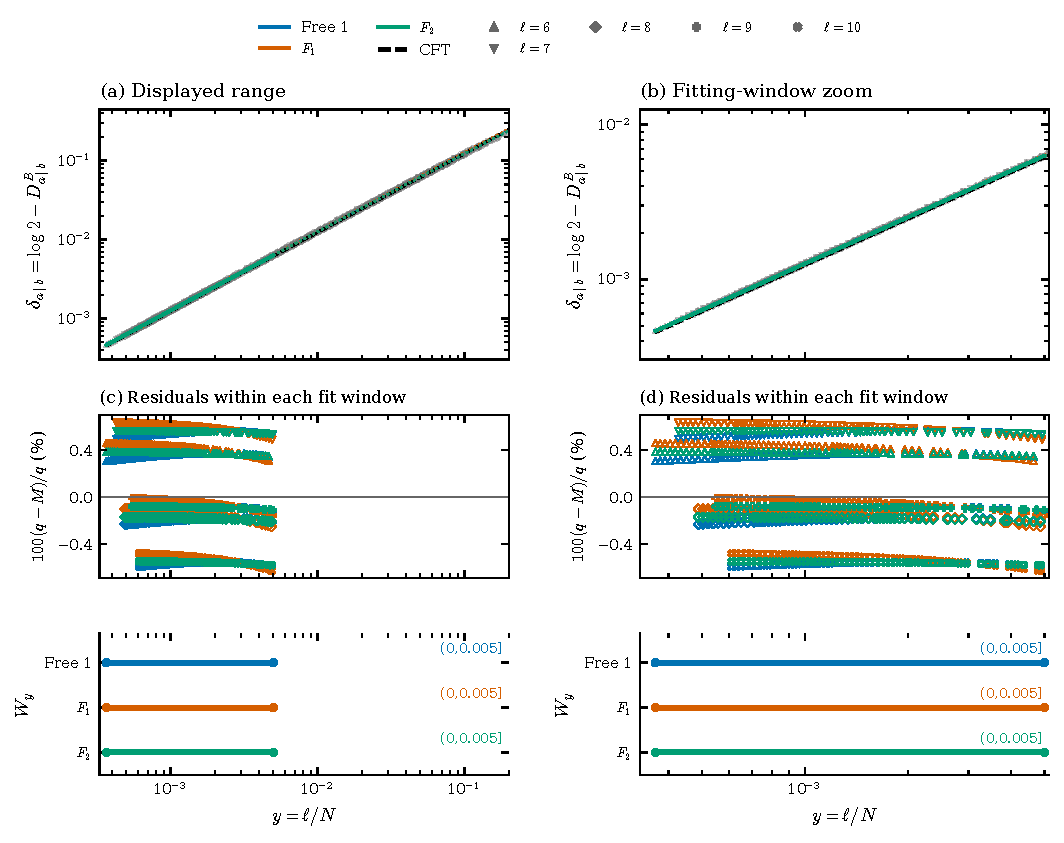
\includegraphics[width=.94\linewidth]{../figs/pair_large_boson_00_ss.pdf}\par\smallskip
\begingroup\scriptsize\setlength{\tabcolsep}{4pt}
\begin{tabular}{lllrrrrr}\toprule
Set & Model & $W_z$ & $m$ & $c_0$ & $r^{(0)}$ & $c_1$ & $r^{(1)}$\\\midrule
Both & Free 1 & $(0,0.005]$ & 317 & 1.2561 & 0.9992554 & --- & ---\\
Both & $F_1$ & $(0,0.005]$ & 317 & 1.2616 & 1 & --- & ---\\
Both & $F_2$ & $(0,0.005]$ & 317 & 1.2627 & 1 & -0.33376 & 2\\
\midrule
Both & CFT & --- & --- & 1.2337 & 1 & --- & ---\\
\bottomrule\end{tabular}
\endgroup
\caption{Compact boson, large intervals, $00\mid ss$, at $p=1/2$, $\ell=6,\ldots,10$, and the complete size grid in Eq.~\eqref{eq:extended-grid}. Here $z=y$ and $q=\delta=\log2-D^B$. Left: all computed data through $z=0.20$; right: a zoom into the common fitting window. Both columns show the same Free 1, $F_1$, and $F_2$ fits. All six directions of this CFT and interval type use the same window. Gray markers denote the data. Colored solid segments lie inside each model\textquotesingle s fitting interval; dotted segments are extrapolations. Black dashed is the analytical CFT leading deficit. The observable axes are logarithmic and span the measured data; nonpositive predictions cannot appear there and out-of-range extrapolations leave the panel. Residual ordinates are linear and show $100(q-M)/q$ only on each model\textquotesingle s fitted observations. Bars give the exact fitting intervals. The parameter block follows Eq.~\eqref{eq:fit}, with $c_0,c_1$ multiplying $z^{r^{(0)}},z^{r^{(1)}}$; all coefficients include powers of $\pi$. A dash means an absent fitted term, or no fitting window for CFT. Values shown are rounded; curves use full precision.}
\label{fig:pair-large_boson-00-ss}
\end{figure}
\begin{figure}[!htbp]\centering
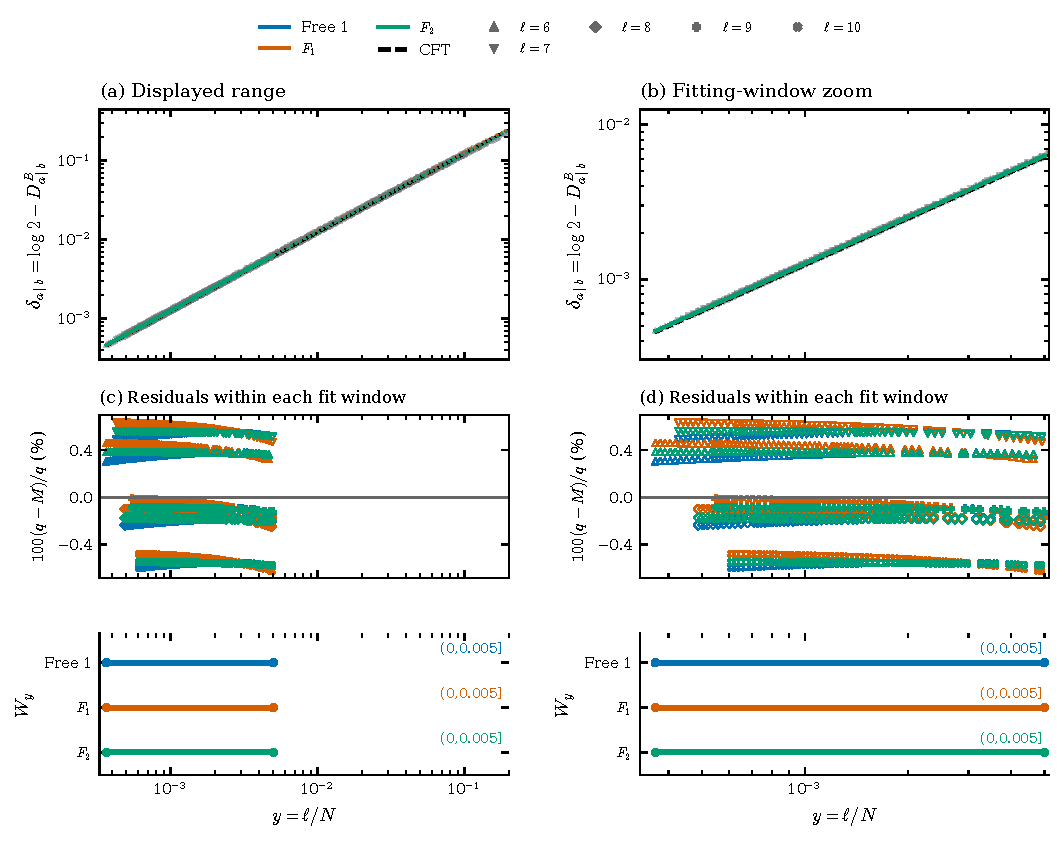
\includegraphics[width=.94\linewidth]{../figs/pair_large_boson_ss_00.pdf}\par\smallskip
\begingroup\scriptsize\setlength{\tabcolsep}{4pt}
\begin{tabular}{lllrrrrr}\toprule
Set & Model & $W_z$ & $m$ & $c_0$ & $r^{(0)}$ & $c_1$ & $r^{(1)}$\\\midrule
Both & Free 1 & $(0,0.005]$ & 317 & 1.256 & 0.9992434 & --- & ---\\
Both & $F_1$ & $(0,0.005]$ & 317 & 1.2616 & 1 & --- & ---\\
Both & $F_2$ & $(0,0.005]$ & 317 & 1.2627 & 1 & -0.34138 & 2\\
\midrule
Both & CFT & --- & --- & 1.2337 & 1 & --- & ---\\
\bottomrule\end{tabular}
\endgroup
\caption{Compact boson, large intervals, $ss\mid 00$, at $p=1/2$, $\ell=6,\ldots,10$, and the complete size grid in Eq.~\eqref{eq:extended-grid}. Here $z=y$ and $q=\delta=\log2-D^B$. Left: all computed data through $z=0.20$; right: a zoom into the common fitting window. Both columns show the same Free 1, $F_1$, and $F_2$ fits. All six directions of this CFT and interval type use the same window. Gray markers denote the data. Colored solid segments lie inside each model\textquotesingle s fitting interval; dotted segments are extrapolations. Black dashed is the analytical CFT leading deficit. The observable axes are logarithmic and span the measured data; nonpositive predictions cannot appear there and out-of-range extrapolations leave the panel. Residual ordinates are linear and show $100(q-M)/q$ only on each model\textquotesingle s fitted observations. Bars give the exact fitting intervals. The parameter block follows Eq.~\eqref{eq:fit}, with $c_0,c_1$ multiplying $z^{r^{(0)}},z^{r^{(1)}}$; all coefficients include powers of $\pi$. A dash means an absent fitted term, or no fitting window for CFT. Values shown are rounded; curves use full precision.}
\label{fig:pair-large_boson-ss-00}
\end{figure}
\begin{figure}[!htbp]\centering
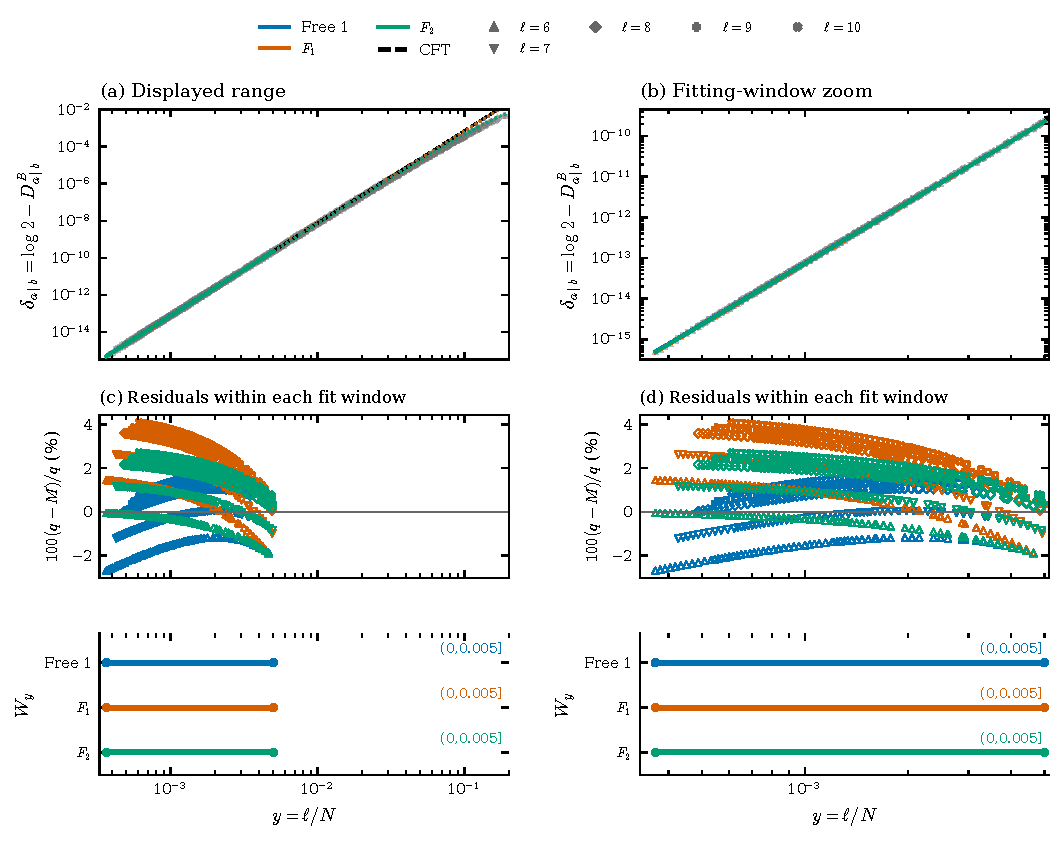
\includegraphics[width=.94\linewidth]{../figs/pair_large_boson_00_3s_s.pdf}\par\smallskip
\begingroup\scriptsize\setlength{\tabcolsep}{4pt}
\begin{tabular}{lllrrrrr}\toprule
Set & Model & $W_z$ & $m$ & $c_0$ & $r^{(0)}$ & $c_1$ & $r^{(1)}$\\\midrule
Both & Free 1 & $(0,0.005]$ & 317 & 66.924 & 4.9836496 & --- & ---\\
Both & $F_1$ & $(0,0.005]$ & 317 & 73.093 & 5 & --- & ---\\
Both & $F_2$ & $(0,0.005]$ & 317 & 74.307 & 5 & -265.58 & 6\\
\midrule
Both & CFT & --- & --- & 75.109 & 5 & --- & ---\\
\bottomrule\end{tabular}
\endgroup
\caption{Compact boson, large intervals, $00\mid 3s,s$, at $p=1/2$, $\ell=6,\ldots,10$, and the complete size grid in Eq.~\eqref{eq:extended-grid}. Here $z=y$ and $q=\delta=\log2-D^B$. Left: all computed data through $z=0.20$; right: a zoom into the common fitting window. Both columns show the same Free 1, $F_1$, and $F_2$ fits. All six directions of this CFT and interval type use the same window. Gray markers denote the data. Colored solid segments lie inside each model\textquotesingle s fitting interval; dotted segments are extrapolations. Black dashed is the analytical CFT leading deficit. The observable axes are logarithmic and span the measured data; nonpositive predictions cannot appear there and out-of-range extrapolations leave the panel. Residual ordinates are linear and show $100(q-M)/q$ only on each model\textquotesingle s fitted observations. Bars give the exact fitting intervals. The parameter block follows Eq.~\eqref{eq:fit}, with $c_0,c_1$ multiplying $z^{r^{(0)}},z^{r^{(1)}}$; all coefficients include powers of $\pi$. A dash means an absent fitted term, or no fitting window for CFT. Values shown are rounded; curves use full precision.}
\label{fig:pair-large_boson-00-3s_s}
\end{figure}
\begin{figure}[!htbp]\centering
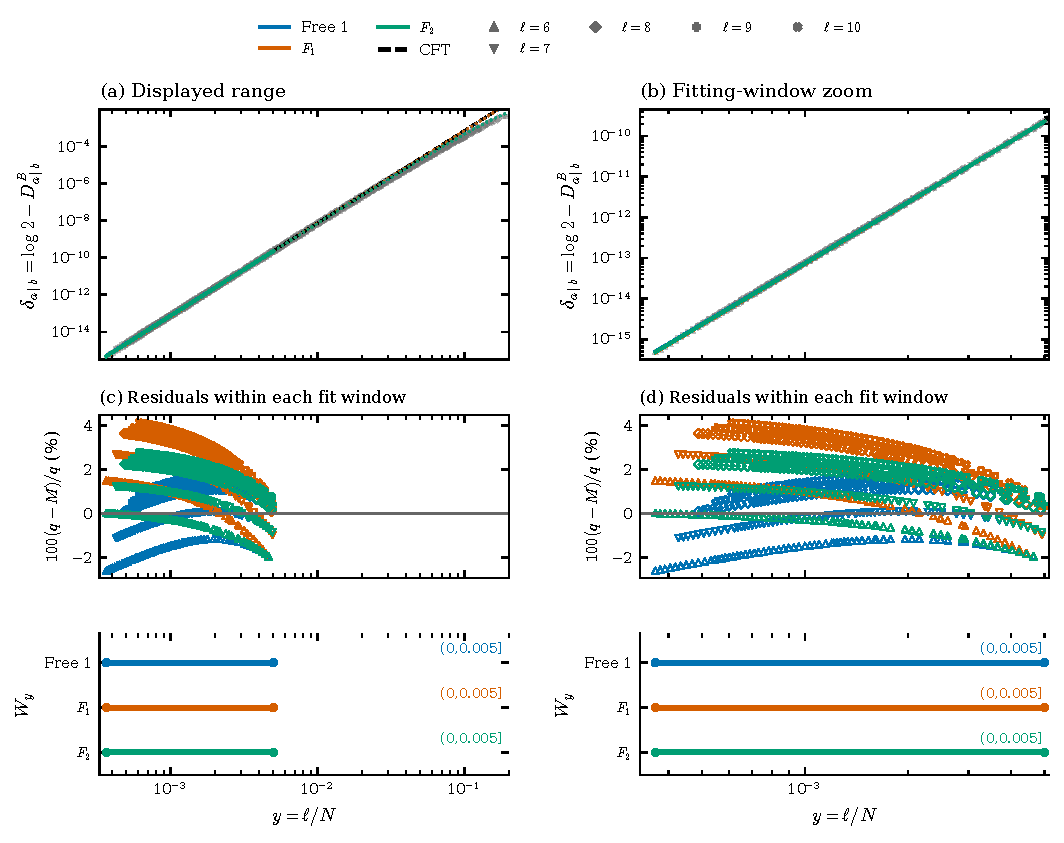
\includegraphics[width=.94\linewidth]{../figs/pair_large_boson_3s_s_00.pdf}\par\smallskip
\begingroup\scriptsize\setlength{\tabcolsep}{4pt}
\begin{tabular}{lllrrrrr}\toprule
Set & Model & $W_z$ & $m$ & $c_0$ & $r^{(0)}$ & $c_1$ & $r^{(1)}$\\\midrule
Both & Free 1 & $(0,0.005]$ & 317 & 66.96 & 4.9838386 & --- & ---\\
Both & $F_1$ & $(0,0.005]$ & 317 & 73.058 & 5 & --- & ---\\
Both & $F_2$ & $(0,0.005]$ & 317 & 74.252 & 5 & -261.18 & 6\\
\midrule
Both & CFT & --- & --- & 75.109 & 5 & --- & ---\\
\bottomrule\end{tabular}
\endgroup
\caption{Compact boson, large intervals, $3s,s\mid 00$, at $p=1/2$, $\ell=6,\ldots,10$, and the complete size grid in Eq.~\eqref{eq:extended-grid}. Here $z=y$ and $q=\delta=\log2-D^B$. Left: all computed data through $z=0.20$; right: a zoom into the common fitting window. Both columns show the same Free 1, $F_1$, and $F_2$ fits. All six directions of this CFT and interval type use the same window. Gray markers denote the data. Colored solid segments lie inside each model\textquotesingle s fitting interval; dotted segments are extrapolations. Black dashed is the analytical CFT leading deficit. The observable axes are logarithmic and span the measured data; nonpositive predictions cannot appear there and out-of-range extrapolations leave the panel. Residual ordinates are linear and show $100(q-M)/q$ only on each model\textquotesingle s fitted observations. Bars give the exact fitting intervals. The parameter block follows Eq.~\eqref{eq:fit}, with $c_0,c_1$ multiplying $z^{r^{(0)}},z^{r^{(1)}}$; all coefficients include powers of $\pi$. A dash means an absent fitted term, or no fitting window for CFT. Values shown are rounded; curves use full precision.}
\label{fig:pair-large_boson-3s_s-00}
\end{figure}
\begin{figure}[!htbp]\centering
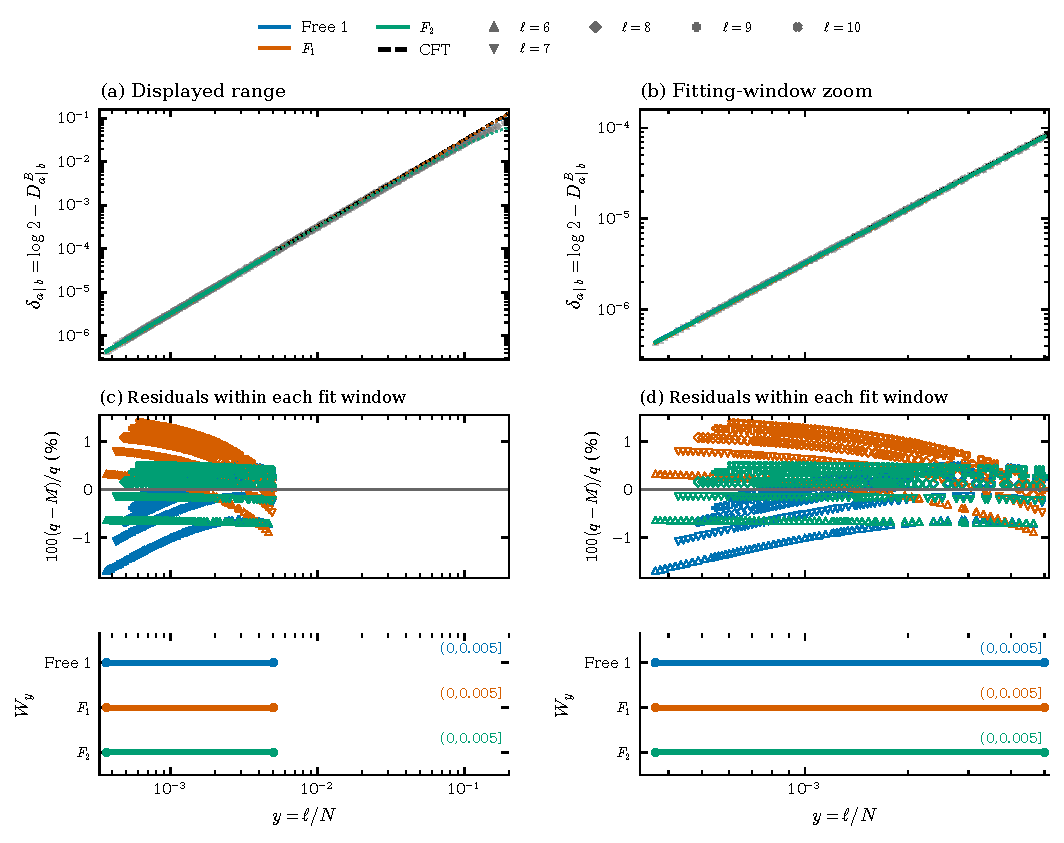
\includegraphics[width=.94\linewidth]{../figs/pair_large_boson_ss_3s_s.pdf}\par\smallskip
\begingroup\scriptsize\setlength{\tabcolsep}{4pt}
\begin{tabular}{lllrrrrr}\toprule
Set & Model & $W_z$ & $m$ & $c_0$ & $r^{(0)}$ & $c_1$ & $r^{(1)}$\\\midrule
Both & Free 1 & $(0,0.005]$ & 317 & 3.069 & 1.9914473 & --- & ---\\
Both & $F_1$ & $(0,0.005]$ & 317 & 3.2185 & 2 & --- & ---\\
Both & $F_2$ & $(0,0.005]$ & 317 & 3.2529 & 2 & -8.6617 & 3\\
\midrule
Both & CFT & --- & --- & 3.2899 & 2 & --- & ---\\
\bottomrule\end{tabular}
\endgroup
\caption{Compact boson, large intervals, $ss\mid 3s,s$, at $p=1/2$, $\ell=6,\ldots,10$, and the complete size grid in Eq.~\eqref{eq:extended-grid}. Here $z=y$ and $q=\delta=\log2-D^B$. Left: all computed data through $z=0.20$; right: a zoom into the common fitting window. Both columns show the same Free 1, $F_1$, and $F_2$ fits. All six directions of this CFT and interval type use the same window. Gray markers denote the data. Colored solid segments lie inside each model\textquotesingle s fitting interval; dotted segments are extrapolations. Black dashed is the analytical CFT leading deficit. The observable axes are logarithmic and span the measured data; nonpositive predictions cannot appear there and out-of-range extrapolations leave the panel. Residual ordinates are linear and show $100(q-M)/q$ only on each model\textquotesingle s fitted observations. Bars give the exact fitting intervals. The parameter block follows Eq.~\eqref{eq:fit}, with $c_0,c_1$ multiplying $z^{r^{(0)}},z^{r^{(1)}}$; all coefficients include powers of $\pi$. A dash means an absent fitted term, or no fitting window for CFT. Values shown are rounded; curves use full precision.}
\label{fig:pair-large_boson-ss-3s_s}
\end{figure}
\begin{figure}[!htbp]\centering
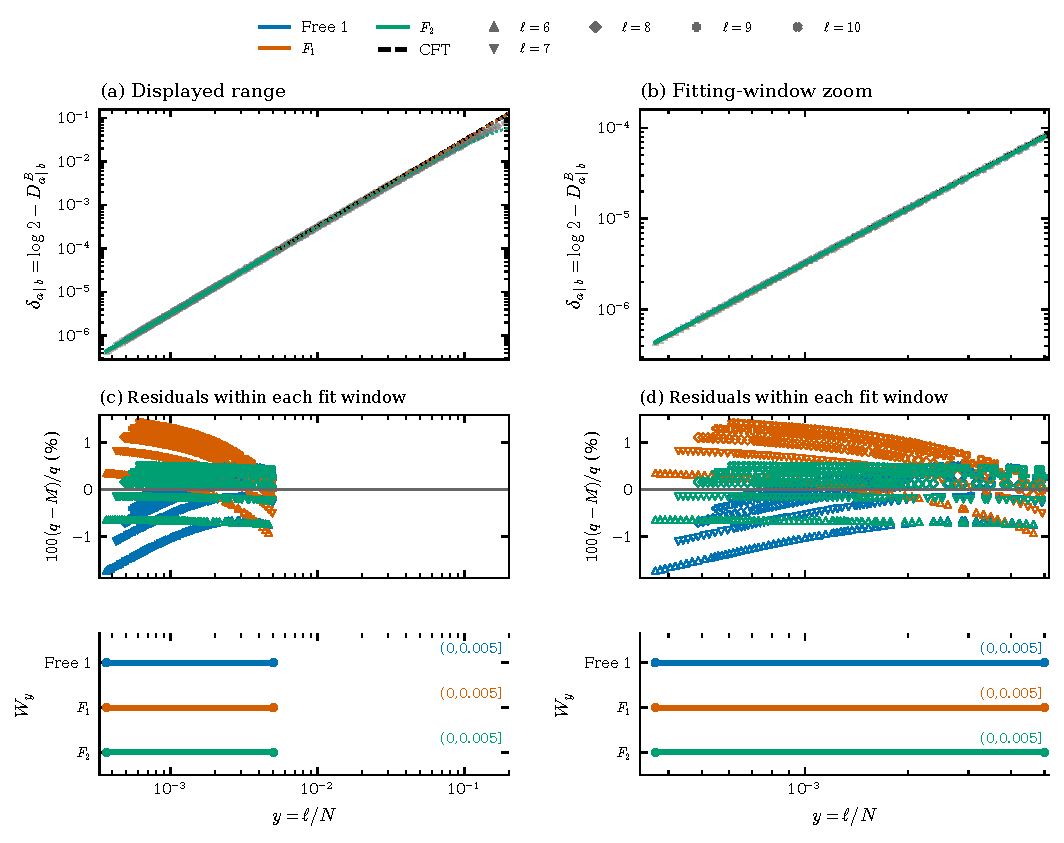
\includegraphics[width=.94\linewidth]{../figs/pair_large_boson_3s_s_ss.pdf}\par\smallskip
\begingroup\scriptsize\setlength{\tabcolsep}{4pt}
\begin{tabular}{lllrrrrr}\toprule
Set & Model & $W_z$ & $m$ & $c_0$ & $r^{(0)}$ & $c_1$ & $r^{(1)}$\\\midrule
Both & Free 1 & $(0,0.005]$ & 317 & 3.0643 & 1.9912306 & --- & ---\\
Both & $F_1$ & $(0,0.005]$ & 317 & 3.2176 & 2 & --- & ---\\
Both & $F_2$ & $(0,0.005]$ & 317 & 3.2528 & 2 & -8.8758 & 3\\
\midrule
Both & CFT & --- & --- & 3.2899 & 2 & --- & ---\\
\bottomrule\end{tabular}
\endgroup
\caption{Compact boson, large intervals, $3s,s\mid ss$, at $p=1/2$, $\ell=6,\ldots,10$, and the complete size grid in Eq.~\eqref{eq:extended-grid}. Here $z=y$ and $q=\delta=\log2-D^B$. Left: all computed data through $z=0.20$; right: a zoom into the common fitting window. Both columns show the same Free 1, $F_1$, and $F_2$ fits. All six directions of this CFT and interval type use the same window. Gray markers denote the data. Colored solid segments lie inside each model\textquotesingle s fitting interval; dotted segments are extrapolations. Black dashed is the analytical CFT leading deficit. The observable axes are logarithmic and span the measured data; nonpositive predictions cannot appear there and out-of-range extrapolations leave the panel. Residual ordinates are linear and show $100(q-M)/q$ only on each model\textquotesingle s fitted observations. Bars give the exact fitting intervals. The parameter block follows Eq.~\eqref{eq:fit}, with $c_0,c_1$ multiplying $z^{r^{(0)}},z^{r^{(1)}}$; all coefficients include powers of $\pi$. A dash means an absent fitted term, or no fitting window for CFT. Values shown are rounded; curves use full precision.}
\label{fig:pair-large_boson-3s_s-ss}
\end{figure}


\appendix
\clearpage
\section{Small-interval fit summaries}
\label{sec:allfits}
The active mixture fits compare a free power law with $F_1,F_2$ and
the supplied analytical CFT series. The models, parameter conversion,
unweighted objective and residual measures are defined in
Sec.~\ref{sec:fits}. Every coefficient includes its power of $\pi$.
The parameter tables group Free, $F_1$, $F_2$, and CFT consecutively
for each ordered pair and give each fitted model's selection interval.
They explicitly give the theoretical leading exponent $\alpha_{\rm CFT}$ and the
analytical coefficients $c_0^{\rm CFT},c_1^{\rm CFT}$ beside the model
coefficients. Only $I\mid\eps$ and $\eps\mid I$ have a supplied
next-order coefficient, respectively $-8\pi^6/45$ and $-8\pi^6/21$
at power six; see Table~\ref{tab:isingcoeff}. A dash in the analytical
next-order column means not supplied, never an assumed zero.
Free, $F_1$, and $F_2$ use the same CFT-wide window in
Eq.~\eqref{eq:common-fit-windows} for every ordered pair.
Sec.~\ref{sec:window-selection} gives a visual comparison for each pair.
All parameters retain full precision in \path{data/f2_summary_fits.csv};
the identical overview-figure fits are in \path{data/scaling_fit_summary.csv}.
The displayed rounding does not enter predictions or residuals.
For a model $M$ with window $W_M$, the quality tables use
\begin{align}
 G_M[\%]&=100\left[1-
 \frac{\mathrm{RMSE}(M;W_M)}{\mathrm{RMSE}(F_1^{[W_M]};W_M)}\right],\nonumber\\
 G_{M,\mathrm{CV}}[\%]&=100\left[1-
 \frac{\mathrm{CVRMSE}(M;W_M)}{\mathrm{CVRMSE}(F_1^{[W_M]};W_M)}\right].
 \label{eq:table-window-gains}
\end{align}
Here $F_1^{[W_M]}$ means that the one-term model is refitted on the
same observations as $M$, also within each omitted-size fold.
For fitted models, its denominator equals the displayed $F_1$ row
because the current windows coincide. The analytical CFT residual
uses these same observations. Raw RMSEs from different windows are
not directly comparable.
\subsection{Ising}
\label{sec:ising-fit-tables}
\begingroup\footnotesize\setlength{\tabcolsep}{3pt}
\begingroup\setlength{\tabcolsep}{2pt}
\begin{longtable}{lllrrrrrrrrr}
\caption{Ising small-interval parameters at $p=1/2$, $\ell=6,\ldots,10$, and the grid in Eq.~\eqref{eq:extended-grid}. Models are grouped by ordered pair. The column $W_x$ gives each fitted model\textquotesingle s interval; CFT adjusts no parameter and has no fitting window. Free, $F_1$, and $F_2$ use the same displayed interval for all six ordered pairs of this CFT and interval type, so the additional term is tested on identical observations. Every model is visualized for each ordered pair in Sec.~\ref{sec:pair-small_ising}. All amplitudes multiply $x^r$ itself and include powers of $\pi$. Columns $c_0,c_1$ multiply the displayed powers $r^{(0)},r^{(1)}$; a dash indicates an absent term. Analytical columns give the complete supplied coefficients. A dash in $c_1^{\rm CFT}$ means that the manuscript does not supply that coefficient, not that it vanishes. Percentage discrepancies follow Eq.~\eqref{eq:metrics}; an imposed power has no estimated exponent discrepancy.}
\label{tab:ising-small-parameters}\\\toprule
Direction & Model & $W_x$ & $\alpha_{\rm CFT}$ & $r^{(0)}$ & $c_0^{\rm CFT}$ & $c_0$ & $r^{(1)}$ & $c_1^{\rm CFT}$ & $c_1$ & $\eta_c$ [\%] & $\eta_r$ [\%]\\\midrule
\endfirsthead
\toprule
Direction & Model & $W_x$ & $\alpha_{\rm CFT}$ & $r^{(0)}$ & $c_0^{\rm CFT}$ & $c_0$ & $r^{(1)}$ & $c_1^{\rm CFT}$ & $c_1$ & $\eta_c$ [\%] & $\eta_r$ [\%]\\\midrule
\endhead
\bottomrule\endfoot
$I\mid \sigma$ & Free & $(0,0.02]$ & 2 & 2.0001 & 0.20562 & 0.20585 & --- & --- & --- & 0.1146 & 0.0070964\\*
$I\mid \sigma$ & $F_1$ & $(0,0.02]$ & 2 & 2 & 0.20562 & 0.20573 & --- & --- & --- & 0.055265 & ---\\*
$I\mid \sigma$ & $F_2$ & $(0,0.02]$ & 2 & 2 & 0.20562 & 0.20571 & 4 & --- & 0.083833 & 0.044771 & ---\\*
$I\mid \sigma$ & CFT & --- & 2 & 2 & 0.20562 & 0.20562 & --- & --- & --- & 0 & ---\\
\midrule
$\sigma\mid I$ & Free & $(0,0.02]$ & 2 & 2.0001 & 0.20562 & 0.20582 & --- & --- & --- & 0.099239 & 0.0057066\\*
$\sigma\mid I$ & $F_1$ & $(0,0.02]$ & 2 & 2 & 0.20562 & 0.20572 & --- & --- & --- & 0.051526 & ---\\*
$\sigma\mid I$ & $F_2$ & $(0,0.02]$ & 2 & 2 & 0.20562 & 0.2057 & 4 & --- & 0.069099 & 0.042877 & ---\\*
$\sigma\mid I$ & CFT & --- & 2 & 2 & 0.20562 & 0.20562 & --- & --- & --- & 0 & ---\\
\midrule
$I\mid \varepsilon$ & Free & $(0,0.02]$ & 4 & 3.9934 & 12.988 & 12.491 & --- & -170.91 & --- & -3.8239 & -0.16507\\*
$I\mid \varepsilon$ & $F_1$ & $(0,0.02]$ & 4 & 4 & 12.988 & 12.83 & --- & -170.91 & --- & -1.219 & ---\\*
$I\mid \varepsilon$ & $F_2$ & $(0,0.02]$ & 4 & 4 & 12.988 & 12.883 & 6 & -170.91 & -170.71 & -0.80492 & ---\\*
$I\mid \varepsilon$ & CFT & --- & 4 & 4 & 12.988 & 12.988 & 6 & -170.91 & -170.91 & 0 & ---\\
\midrule
$\varepsilon\mid I$ & Free & $(0,0.02]$ & 4 & 3.9861 & 12.988 & 12.07 & --- & -366.24 & --- & -7.0661 & -0.34832\\*
$\varepsilon\mid I$ & $F_1$ & $(0,0.02]$ & 4 & 4 & 12.988 & 12.77 & --- & -366.24 & --- & -1.6748 & ---\\*
$\varepsilon\mid I$ & $F_2$ & $(0,0.02]$ & 4 & 4 & 12.988 & 12.882 & 6 & -366.24 & -355.38 & -0.81263 & ---\\*
$\varepsilon\mid I$ & CFT & --- & 4 & 4 & 12.988 & 12.988 & 6 & -366.24 & -366.24 & 0 & ---\\
\midrule
$\sigma\mid \varepsilon$ & Free & $(0,0.02]$ & 2 & 2.0238 & 0.20562 & 0.23069 & --- & --- & --- & 12.192 & 1.1878\\*
$\sigma\mid \varepsilon$ & $F_1$ & $(0,0.02]$ & 2 & 2 & 0.20562 & 0.2089 & --- & --- & --- & 1.595 & ---\\*
$\sigma\mid \varepsilon$ & $F_2$ & $(0,0.02]$ & 2 & 2 & 0.20562 & 0.20565 & 4 & --- & 12.604 & 0.017273 & ---\\*
$\sigma\mid \varepsilon$ & CFT & --- & 2 & 2 & 0.20562 & 0.20562 & --- & --- & --- & 0 & ---\\
\midrule
$\varepsilon\mid \sigma$ & Free & $(0,0.02]$ & 2 & 2.0176 & 0.20562 & 0.22393 & --- & --- & --- & 8.9077 & 0.88006\\*
$\varepsilon\mid \sigma$ & $F_1$ & $(0,0.02]$ & 2 & 2 & 0.20562 & 0.20806 & --- & --- & --- & 1.1882 & ---\\*
$\varepsilon\mid \sigma$ & $F_2$ & $(0,0.02]$ & 2 & 2 & 0.20562 & 0.20566 & 4 & --- & 9.3133 & 0.022414 & ---\\*
$\varepsilon\mid \sigma$ & CFT & --- & 2 & 2 & 0.20562 & 0.20562 & --- & --- & --- & 0 & ---\\
\end{longtable}
\endgroup

\begingroup\setlength{\tabcolsep}{2pt}
\begin{longtable}{lllrrrrrrr}
\caption{Ising small-interval fit quality for Table~\ref{tab:ising-small-parameters}, in the same ordered-pair blocks. All fitted-row metrics use that row\textquotesingle s $W_x$ and $m$ observations; $k$ is the fitted parameter count. CFT metrics are evaluated on the same displayed window as the fitted rows, although no fitting is performed. RMSE, CV RMSE, and RMSrel follow Eqs.~\eqref{eq:metrics} and \eqref{eq:cv}. For every $F_2$ row, gains $G,G_{\rm CV}$ use $F_1$ refitted on exactly that $F_2$ window, as in Eq.~\eqref{eq:table-window-gains}; its denominator equals the displayed $F_1$ row because the windows now match. Negative gains mean worse prediction. Absolute RMSEs on different windows should not be ranked directly.}
\label{tab:ising-small-metrics}\\\toprule
Direction & Model & $W_x$ & $m$ & $k$ & RMSE & CV RMSE & RMSrel [\%] & $G$ [\%] & $G_{\rm CV}$ [\%]\\\midrule
\endfirsthead
\toprule
Direction & Model & $W_x$ & $m$ & $k$ & RMSE & CV RMSE & RMSrel [\%] & $G$ [\%] & $G_{\rm CV}$ [\%]\\\midrule
\endhead
\bottomrule\endfoot
$I\mid \sigma$ & Free & $(0,0.02]$ & 1255 & 2 & $5.158\!\times\!10^{-9}$ & $5.190\!\times\!10^{-9}$ & 0.02149 & 1.7481 & 1.5281\\*
$I\mid \sigma$ & $F_1$ & $(0,0.02]$ & 1255 & 1 & $5.249\!\times\!10^{-9}$ & $5.271\!\times\!10^{-9}$ & 0.017876 & 0 & 0\\*
$I\mid \sigma$ & $F_2$ & $(0,0.02]$ & 1255 & 2 & $5.124\!\times\!10^{-9}$ & $5.161\!\times\!10^{-9}$ & 0.016955 & 2.3911 & 2.077\\*
$I\mid \sigma$ & CFT & --- & 1255 & 0 & $1.719\!\times\!10^{-8}$ & $1.719\!\times\!10^{-8}$ & 0.053178 & -227.43 & -226.11\\
\midrule
$\sigma\mid I$ & Free & $(0,0.02]$ & 1255 & 2 & $4.526\!\times\!10^{-9}$ & $4.554\!\times\!10^{-9}$ & 0.01948 & 1.4739 & 1.2593\\*
$\sigma\mid I$ & $F_1$ & $(0,0.02]$ & 1255 & 1 & $4.594\!\times\!10^{-9}$ & $4.612\!\times\!10^{-9}$ & 0.016173 & 0 & 0\\*
$\sigma\mid I$ & $F_2$ & $(0,0.02]$ & 1255 & 2 & $4.497\!\times\!10^{-9}$ & $4.528\!\times\!10^{-9}$ & 0.01584 & 2.1181 & 1.8149\\*
$\sigma\mid I$ & CFT & --- & 1255 & 0 & $1.594\!\times\!10^{-8}$ & $1.594\!\times\!10^{-8}$ & 0.050669 & -246.9 & -245.54\\
\midrule
$I\mid \varepsilon$ & Free & $(0,0.02]$ & 1255 & 2 & $1.566\!\times\!10^{-9}$ & $1.585\!\times\!10^{-9}$ & 0.81516 & 3.9757 & 3.6364\\*
$I\mid \varepsilon$ & $F_1$ & $(0,0.02]$ & 1255 & 1 & $1.631\!\times\!10^{-9}$ & $1.645\!\times\!10^{-9}$ & 0.38995 & 0 & 0\\*
$I\mid \varepsilon$ & $F_2$ & $(0,0.02]$ & 1255 & 2 & $1.561\!\times\!10^{-9}$ & $1.582\!\times\!10^{-9}$ & 0.33241 & 4.2923 & 3.8386\\*
$I\mid \varepsilon$ & CFT & --- & 1255 & 0 & $4.411\!\times\!10^{-9}$ & $4.411\!\times\!10^{-9}$ & 0.94868 & -170.42 & -168.19\\
\midrule
$\varepsilon\mid I$ & Free & $(0,0.02]$ & 1255 & 2 & $1.565\!\times\!10^{-9}$ & $1.583\!\times\!10^{-9}$ & 1.544 & 14.705 & 14.389\\*
$\varepsilon\mid I$ & $F_1$ & $(0,0.02]$ & 1255 & 1 & $1.834\!\times\!10^{-9}$ & $1.849\!\times\!10^{-9}$ & 0.65255 & 0 & 0\\*
$\varepsilon\mid I$ & $F_2$ & $(0,0.02]$ & 1255 & 2 & $1.548\!\times\!10^{-9}$ & $1.568\!\times\!10^{-9}$ & 0.33073 & 15.616 & 15.195\\*
$\varepsilon\mid I$ & CFT & --- & 1255 & 0 & $4.320\!\times\!10^{-9}$ & $4.320\!\times\!10^{-9}$ & 0.94559 & -135.49 & -133.62\\
\midrule
$\sigma\mid \varepsilon$ & Free & $(0,0.02]$ & 1255 & 2 & $4.655\!\times\!10^{-8}$ & $4.675\!\times\!10^{-8}$ & 2.1632 & 72.895 & 72.862\\*
$\sigma\mid \varepsilon$ & $F_1$ & $(0,0.02]$ & 1255 & 1 & $1.717\!\times\!10^{-7}$ & $1.723\!\times\!10^{-7}$ & 1.1334 & 0 & 0\\*
$\sigma\mid \varepsilon$ & $F_2$ & $(0,0.02]$ & 1255 & 2 & $7.741\!\times\!10^{-9}$ & $7.820\!\times\!10^{-9}$ & 0.018834 & 95.492 & 95.461\\*
$\sigma\mid \varepsilon$ & CFT & --- & 1255 & 0 & $5.026\!\times\!10^{-7}$ & $5.026\!\times\!10^{-7}$ & 0.88172 & -192.67 & -191.78\\
\midrule
$\varepsilon\mid \sigma$ & Free & $(0,0.02]$ & 1255 & 2 & $3.468\!\times\!10^{-8}$ & $3.483\!\times\!10^{-8}$ & 1.6121 & 72.684 & 72.651\\*
$\varepsilon\mid \sigma$ & $F_1$ & $(0,0.02]$ & 1255 & 1 & $1.270\!\times\!10^{-7}$ & $1.274\!\times\!10^{-7}$ & 0.83808 & 0 & 0\\*
$\varepsilon\mid \sigma$ & $F_2$ & $(0,0.02]$ & 1255 & 2 & $7.163\!\times\!10^{-9}$ & $7.236\!\times\!10^{-9}$ & 0.016596 & 94.359 & 94.318\\*
$\varepsilon\mid \sigma$ & CFT & --- & 1255 & 0 & $3.741\!\times\!10^{-7}$ & $3.741\!\times\!10^{-7}$ & 0.66099 & -194.64 & -193.74\\
\end{longtable}
\endgroup

\endgroup
\subsection{Compact boson}
\label{sec:boson-fit-tables}
\begingroup\footnotesize\setlength{\tabcolsep}{3pt}
\begingroup\setlength{\tabcolsep}{2pt}
\begin{longtable}{lllrrrrrrrrr}
\caption{Compact boson small-interval parameters at $p=1/2$, $\ell=6,\ldots,10$, and the grid in Eq.~\eqref{eq:extended-grid}. Models are grouped by ordered pair. The column $W_x$ gives each fitted model\textquotesingle s interval; CFT adjusts no parameter and has no fitting window. Free, $F_1$, and $F_2$ use the same displayed interval for all six ordered pairs of this CFT and interval type, so the additional term is tested on identical observations. Every model is visualized for each ordered pair in Sec.~\ref{sec:pair-small_boson}. All amplitudes multiply $x^r$ itself and include powers of $\pi$. Columns $c_0,c_1$ multiply the displayed powers $r^{(0)},r^{(1)}$; a dash indicates an absent term. Analytical columns give the complete supplied coefficients. A dash in $c_1^{\rm CFT}$ means that the manuscript does not supply that coefficient, not that it vanishes. Percentage discrepancies follow Eq.~\eqref{eq:metrics}; an imposed power has no estimated exponent discrepancy.}
\label{tab:boson-small-parameters}\\\toprule
Direction & Model & $W_x$ & $\alpha_{\rm CFT}$ & $r^{(0)}$ & $c_0^{\rm CFT}$ & $c_0$ & $r^{(1)}$ & $c_1^{\rm CFT}$ & $c_1$ & $\eta_c$ [\%] & $\eta_r$ [\%]\\\midrule
\endfirsthead
\toprule
Direction & Model & $W_x$ & $\alpha_{\rm CFT}$ & $r^{(0)}$ & $c_0^{\rm CFT}$ & $c_0$ & $r^{(1)}$ & $c_1^{\rm CFT}$ & $c_1$ & $\eta_c$ [\%] & $\eta_r$ [\%]\\\midrule
\endhead
\bottomrule\endfoot
$00\mid ss$ & Free & $(0,0.1]$ & 2 & 1.9982 & 0.82247 & 0.77501 & --- & --- & --- & -5.7697 & -0.092048\\*
$00\mid ss$ & $F_1$ & $(0,0.1]$ & 2 & 2 & 0.82247 & 0.77866 & --- & --- & --- & -5.3266 & ---\\*
$00\mid ss$ & $F_2$ & $(0,0.1]$ & 2 & 2 & 0.82247 & 0.77996 & 4 & --- & -0.1917 & -5.1687 & ---\\*
$00\mid ss$ & CFT & --- & 2 & 2 & 0.82247 & 0.82247 & --- & --- & --- & 0 & ---\\
\midrule
$ss\mid 00$ & Free & $(0,0.1]$ & 2 & 1.9983 & 0.82247 & 0.77529 & --- & --- & --- & -5.7362 & -0.086511\\*
$ss\mid 00$ & $F_1$ & $(0,0.1]$ & 2 & 2 & 0.82247 & 0.77871 & --- & --- & --- & -5.3197 & ---\\*
$ss\mid 00$ & $F_2$ & $(0,0.1]$ & 2 & 2 & 0.82247 & 0.77995 & 4 & --- & -0.18219 & -5.1696 & ---\\*
$ss\mid 00$ & CFT & --- & 2 & 2 & 0.82247 & 0.82247 & --- & --- & --- & 0 & ---\\
\midrule
$00\mid 3s,s$ & Free & $(0,0.1]$ & 2 & 1.9649 & 4.1123 & 3.5315 & --- & --- & --- & -14.124 & -1.7561\\*
$00\mid 3s,s$ & $F_1$ & $(0,0.1]$ & 2 & 2 & 4.1123 & 3.8623 & --- & --- & --- & -6.0813 & ---\\*
$00\mid 3s,s$ & $F_2$ & $(0,0.1]$ & 2 & 2 & 4.1123 & 3.964 & 4 & --- & -15.02 & -3.6065 & ---\\*
$00\mid 3s,s$ & CFT & --- & 2 & 2 & 4.1123 & 4.1123 & --- & --- & --- & 0 & ---\\
\midrule
$3s,s\mid 00$ & Free & $(0,0.1]$ & 2 & 1.966 & 4.1123 & 3.545 & --- & --- & --- & -13.795 & -1.6988\\*
$3s,s\mid 00$ & $F_1$ & $(0,0.1]$ & 2 & 2 & 4.1123 & 3.8657 & --- & --- & --- & -5.9968 & ---\\*
$3s,s\mid 00$ & $F_2$ & $(0,0.1]$ & 2 & 2 & 4.1123 & 3.9643 & 4 & --- & -14.541 & -3.6009 & ---\\*
$3s,s\mid 00$ & CFT & --- & 2 & 2 & 4.1123 & 4.1123 & --- & --- & --- & 0 & ---\\
\midrule
$ss\mid 3s,s$ & Free & $(0,0.1]$ & 2 & 1.9883 & 1.6449 & 1.5661 & --- & --- & --- & -4.7937 & -0.58466\\*
$ss\mid 3s,s$ & $F_1$ & $(0,0.1]$ & 2 & 2 & 1.6449 & 1.6134 & --- & --- & --- & -1.9141 & ---\\*
$ss\mid 3s,s$ & $F_2$ & $(0,0.1]$ & 2 & 2 & 1.6449 & 1.6276 & 4 & --- & -2.0896 & -1.0534 & ---\\*
$ss\mid 3s,s$ & CFT & --- & 2 & 2 & 1.6449 & 1.6449 & --- & --- & --- & 0 & ---\\
\midrule
$3s,s\mid ss$ & Free & $(0,0.1]$ & 2 & 1.9902 & 1.6449 & 1.576 & --- & --- & --- & -4.1922 & -0.48899\\*
$3s,s\mid ss$ & $F_1$ & $(0,0.1]$ & 2 & 2 & 1.6449 & 1.6157 & --- & --- & --- & -1.7746 & ---\\*
$3s,s\mid ss$ & $F_2$ & $(0,0.1]$ & 2 & 2 & 1.6449 & 1.6276 & 4 & --- & -1.7507 & -1.0534 & ---\\*
$3s,s\mid ss$ & CFT & --- & 2 & 2 & 1.6449 & 1.6449 & --- & --- & --- & 0 & ---\\
\end{longtable}
\endgroup

\begingroup\setlength{\tabcolsep}{2pt}
\begin{longtable}{lllrrrrrrr}
\caption{Compact boson small-interval fit quality for Table~\ref{tab:boson-small-parameters}, in the same ordered-pair blocks. All fitted-row metrics use that row\textquotesingle s $W_x$ and $m$ observations; $k$ is the fitted parameter count. CFT metrics are evaluated on the same displayed window as the fitted rows, although no fitting is performed. RMSE, CV RMSE, and RMSrel follow Eqs.~\eqref{eq:metrics} and \eqref{eq:cv}. For every $F_2$ row, gains $G,G_{\rm CV}$ use $F_1$ refitted on exactly that $F_2$ window, as in Eq.~\eqref{eq:table-window-gains}; its denominator equals the displayed $F_1$ row because the windows now match. Negative gains mean worse prediction. Absolute RMSEs on different windows should not be ranked directly.}
\label{tab:boson-small-metrics}\\\toprule
Direction & Model & $W_x$ & $m$ & $k$ & RMSE & CV RMSE & RMSrel [\%] & $G$ [\%] & $G_{\rm CV}$ [\%]\\\midrule
\endfirsthead
\toprule
Direction & Model & $W_x$ & $m$ & $k$ & RMSE & CV RMSE & RMSrel [\%] & $G$ [\%] & $G_{\rm CV}$ [\%]\\\midrule
\endhead
\bottomrule\endfoot
$00\mid ss$ & Free & $(0,0.1]$ & 598 & 2 & $1.742\!\times\!10^{-5}$ & $1.819\!\times\!10^{-5}$ & 1.2305 & 0.094877 & -1.6624\\*
$00\mid ss$ & $F_1$ & $(0,0.1]$ & 598 & 1 & $1.744\!\times\!10^{-5}$ & $1.790\!\times\!10^{-5}$ & 1.0961 & 0 & 0\\*
$00\mid ss$ & $F_2$ & $(0,0.1]$ & 598 & 2 & $1.741\!\times\!10^{-5}$ & $1.835\!\times\!10^{-5}$ & 1.0996 & 0.15988 & -2.5678\\*
$00\mid ss$ & CFT & --- & 598 & 0 & $9.183\!\times\!10^{-5}$ & $9.183\!\times\!10^{-5}$ & 5.6824 & -426.7 & -413.16\\
\midrule
$ss\mid 00$ & Free & $(0,0.1]$ & 598 & 2 & $1.737\!\times\!10^{-5}$ & $1.814\!\times\!10^{-5}$ & 1.2171 & 0.084288 & -1.6754\\*
$ss\mid 00$ & $F_1$ & $(0,0.1]$ & 598 & 1 & $1.739\!\times\!10^{-5}$ & $1.784\!\times\!10^{-5}$ & 1.0955 & 0 & 0\\*
$ss\mid 00$ & $F_2$ & $(0,0.1]$ & 598 & 2 & $1.736\!\times\!10^{-5}$ & $1.830\!\times\!10^{-5}$ & 1.0992 & 0.14523 & -2.5842\\*
$ss\mid 00$ & CFT & --- & 598 & 0 & $9.171\!\times\!10^{-5}$ & $9.171\!\times\!10^{-5}$ & 5.6814 & -427.5 & -413.98\\
\midrule
$00\mid 3s,s$ & Free & $(0,0.1]$ & 598 & 2 & $6.866\!\times\!10^{-5}$ & $7.172\!\times\!10^{-5}$ & 9.5493 & 31.286 & 30.43\\*
$00\mid 3s,s$ & $F_1$ & $(0,0.1]$ & 598 & 1 & $9.993\!\times\!10^{-5}$ & $1.031\!\times\!10^{-4}$ & 2.5019 & 0 & 0\\*
$00\mid 3s,s$ & $F_2$ & $(0,0.1]$ & 598 & 2 & $6.343\!\times\!10^{-5}$ & $6.680\!\times\!10^{-5}$ & 0.81386 & 36.528 & 35.203\\*
$00\mid 3s,s$ & CFT & --- & 598 & 0 & $5.243\!\times\!10^{-4}$ & $5.243\!\times\!10^{-4}$ & 4.2262 & -424.67 & -408.57\\
\midrule
$3s,s\mid 00$ & Free & $(0,0.1]$ & 598 & 2 & $6.562\!\times\!10^{-5}$ & $6.848\!\times\!10^{-5}$ & 9.2257 & 31.748 & 30.941\\*
$3s,s\mid 00$ & $F_1$ & $(0,0.1]$ & 598 & 1 & $9.614\!\times\!10^{-5}$ & $9.916\!\times\!10^{-5}$ & 2.4246 & 0 & 0\\*
$3s,s\mid 00$ & $F_2$ & $(0,0.1]$ & 598 & 2 & $6.045\!\times\!10^{-5}$ & $6.360\!\times\!10^{-5}$ & 0.80915 & 37.118 & 35.866\\*
$3s,s\mid 00$ & CFT & --- & 598 & 0 & $5.166\!\times\!10^{-4}$ & $5.166\!\times\!10^{-4}$ & 4.2085 & -437.29 & -420.93\\
\midrule
$ss\mid 3s,s$ & Free & $(0,0.1]$ & 598 & 2 & $1.453\!\times\!10^{-5}$ & $1.519\!\times\!10^{-5}$ & 3.0938 & 17.691 & 16.67\\*
$ss\mid 3s,s$ & $F_1$ & $(0,0.1]$ & 598 & 1 & $1.765\!\times\!10^{-5}$ & $1.823\!\times\!10^{-5}$ & 0.87666 & 0 & 0\\*
$ss\mid 3s,s$ & $F_2$ & $(0,0.1]$ & 598 & 2 & $1.400\!\times\!10^{-5}$ & $1.476\!\times\!10^{-5}$ & 0.41654 & 20.66 & 18.998\\*
$ss\mid 3s,s$ & CFT & --- & 598 & 0 & $6.716\!\times\!10^{-5}$ & $6.716\!\times\!10^{-5}$ & 1.2933 & -280.54 & -268.48\\
\midrule
$3s,s\mid ss$ & Free & $(0,0.1]$ & 598 & 2 & $1.241\!\times\!10^{-5}$ & $1.294\!\times\!10^{-5}$ & 2.5931 & 17.149 & 16.297\\*
$3s,s\mid ss$ & $F_1$ & $(0,0.1]$ & 598 & 1 & $1.498\!\times\!10^{-5}$ & $1.546\!\times\!10^{-5}$ & 0.76126 & 0 & 0\\*
$3s,s\mid ss$ & $F_2$ & $(0,0.1]$ & 598 & 2 & $1.198\!\times\!10^{-5}$ & $1.258\!\times\!10^{-5}$ & 0.40929 & 20.054 & 18.631\\*
$3s,s\mid ss$ & CFT & --- & 598 & 0 & $6.191\!\times\!10^{-5}$ & $6.191\!\times\!10^{-5}$ & 1.2671 & -313.26 & -300.6\\
\end{longtable}
\endgroup

\endgroup
\clearpage
\section{Large-interval fit summaries and sanity checks}
\label{sec:complement-checks}

\subsection{Separate free, one-term, and two-term fits}
\label{sec:complement-fit-tables}
Every coefficient multiplies $y^r$ itself. Free fits determine amplitude
and exponent; $F_1$ fixes the analytical leading exponent and fits one
amplitude; $F_2$ fixes the leading and next powers in
Table~\ref{tab:complement-theory} and fits both amplitudes.
The CFT leading rows adjust no parameter. Free, $F_1$, and $F_2$ share
the CFT-wide window in Eq.~\eqref{eq:common-fit-windows} for all
six directions. The boson window is provisional; see
Appendix~\ref{sec:common-window-results}. All fits use $\ell=6,\ldots,10$,
the grid in Eq.~\eqref{eq:extended-grid}, and the
objective and diagnostics in Sec.~\ref{sec:fits}. The parameter tables
repeat the analytical leading coefficient $c_0^{\rm CFT}$ beside each
model amplitude. Their $c_1^{\rm CFT}$ column contains dashes because
the manuscript supplies no next-order coefficient for these large-interval
pairs. The next powers used in $F_2$ remain those in
Table~\ref{tab:complement-theory}, including its qualification that
the boson $ss\leftrightarrow(3s,s)$ power three is an allowed sector.
The quality-table gains use the matching-window $F_1$ reference in
Eq.~\eqref{eq:table-window-gains}; CFT metrics are evaluated on
the same CFT-wide window. The per-pair figures in Sec.~\ref{sec:window-selection}
show the corresponding curves and fitting intervals.
\begingroup\footnotesize\setlength{\tabcolsep}{3pt}
\begingroup\setlength{\tabcolsep}{2pt}
\begin{longtable}{lllrrrrrrrrr}
\caption{Ising large-interval parameters at $p=1/2$, $\ell=6,\ldots,10$, and the grid in Eq.~\eqref{eq:extended-grid}. Models are grouped by ordered pair. The column $W_y$ gives each fitted model\textquotesingle s interval; CFT adjusts no parameter and has no fitting window. Free, $F_1$, and $F_2$ use the same displayed interval for all six ordered pairs of this CFT and interval type, so the additional term is tested on identical observations. Every model is visualized for each ordered pair in Sec.~\ref{sec:pair-large_ising}. All amplitudes multiply $y^r$ itself and include powers of $\pi$. Columns $c_0,c_1$ multiply the displayed powers $r^{(0)},r^{(1)}$; a dash indicates an absent term. Analytical columns give the complete supplied coefficients. A dash in $c_1^{\rm CFT}$ means that the manuscript does not supply that coefficient, not that it vanishes. Percentage discrepancies follow Eq.~\eqref{eq:metrics}; an imposed power has no estimated exponent discrepancy.}
\label{tab:ising-large-parameters}\\\toprule
Direction & Model & $W_y$ & $\beta_{\rm CFT}$ & $r^{(0)}$ & $c_0^{\rm CFT}$ & $c_0$ & $r^{(1)}$ & $c_1^{\rm CFT}$ & $c_1$ & $\eta_c$ [\%] & $\eta_r$ [\%]\\\midrule
\endfirsthead
\toprule
Direction & Model & $W_y$ & $\beta_{\rm CFT}$ & $r^{(0)}$ & $c_0^{\rm CFT}$ & $c_0$ & $r^{(1)}$ & $c_1^{\rm CFT}$ & $c_1$ & $\eta_c$ [\%] & $\eta_r$ [\%]\\\midrule
\endhead
\bottomrule\endfoot
$I\mid \sigma$ & Free & $(0,0.002]$ & 0.25 & 0.26465 & 0.61965 & 0.71994 & --- & --- & --- & 16.184 & 5.8606\\*
$I\mid \sigma$ & $F_1$ & $(0,0.002]$ & 0.25 & 0.25 & 0.61965 & 0.65339 & --- & --- & --- & 5.4442 & ---\\*
$I\mid \sigma$ & $F_2$ & $(0,0.002]$ & 0.25 & 0.25 & 0.61965 & 0.61463 & 0.5 & --- & 0.20243 & -0.81098 & ---\\*
$I\mid \sigma$ & CFT & --- & 0.25 & 0.25 & 0.61965 & 0.61965 & --- & --- & --- & 0 & ---\\
\midrule
$\sigma\mid I$ & Free & $(0,0.002]$ & 0.25 & 0.26465 & 0.61965 & 0.71995 & --- & --- & --- & 16.186 & 5.8612\\*
$\sigma\mid I$ & $F_1$ & $(0,0.002]$ & 0.25 & 0.25 & 0.61965 & 0.65339 & --- & --- & --- & 5.4445 & ---\\*
$\sigma\mid I$ & $F_2$ & $(0,0.002]$ & 0.25 & 0.25 & 0.61965 & 0.61462 & 0.5 & --- & 0.20245 & -0.81139 & ---\\*
$\sigma\mid I$ & CFT & --- & 0.25 & 0.25 & 0.61965 & 0.61965 & --- & --- & --- & 0 & ---\\
\midrule
$I\mid \varepsilon$ & Free & $(0,0.002]$ & 2 & 1.9985 & 3.2899 & 3.2548 & --- & --- & --- & -1.0674 & -0.074487\\*
$I\mid \varepsilon$ & $F_1$ & $(0,0.002]$ & 2 & 2 & 3.2899 & 3.2861 & --- & --- & --- & -0.11533 & ---\\*
$I\mid \varepsilon$ & $F_2$ & $(0,0.002]$ & 2 & 2 & 3.2899 & 3.289 & 4 & --- & -1070.2 & -0.024918 & ---\\*
$I\mid \varepsilon$ & CFT & --- & 2 & 2 & 3.2899 & 3.2899 & --- & --- & --- & 0 & ---\\
\midrule
$\varepsilon\mid I$ & Free & $(0,0.002]$ & 2 & 2.0013 & 3.2899 & 3.3242 & --- & --- & --- & 1.0443 & 0.065315\\*
$\varepsilon\mid I$ & $F_1$ & $(0,0.002]$ & 2 & 2 & 3.2899 & 3.2964 & --- & --- & --- & 0.19921 & ---\\*
$\varepsilon\mid I$ & $F_2$ & $(0,0.002]$ & 2 & 2 & 3.2899 & 3.2938 & 4 & --- & 959.21 & 0.11818 & ---\\*
$\varepsilon\mid I$ & CFT & --- & 2 & 2 & 3.2899 & 3.2899 & --- & --- & --- & 0 & ---\\
\midrule
$\sigma\mid \varepsilon$ & Free & $(0,0.002]$ & 0.25 & 0.25058 & 0.15491 & 0.15691 & --- & --- & --- & 1.2904 & 0.23227\\*
$\sigma\mid \varepsilon$ & $F_1$ & $(0,0.002]$ & 0.25 & 0.25 & 0.15491 & 0.15631 & --- & --- & --- & 0.9017 & ---\\*
$\sigma\mid \varepsilon$ & $F_2$ & $(0,0.002]$ & 0.25 & 0.25 & 0.15491 & 0.15595 & 0.5 & --- & 0.0018716 & 0.67037 & ---\\*
$\sigma\mid \varepsilon$ & CFT & --- & 0.25 & 0.25 & 0.15491 & 0.15491 & --- & --- & --- & 0 & ---\\
\midrule
$\varepsilon\mid \sigma$ & Free & $(0,0.002]$ & 0.25 & 0.25544 & 0.15491 & 0.16288 & --- & --- & --- & 5.1411 & 2.1754\\*
$\varepsilon\mid \sigma$ & $F_1$ & $(0,0.002]$ & 0.25 & 0.25 & 0.15491 & 0.15712 & --- & --- & --- & 1.4228 & ---\\*
$\varepsilon\mid \sigma$ & $F_2$ & $(0,0.002]$ & 0.25 & 0.25 & 0.15491 & 0.15365 & 0.5 & --- & 0.018087 & -0.81285 & ---\\*
$\varepsilon\mid \sigma$ & CFT & --- & 0.25 & 0.25 & 0.15491 & 0.15491 & --- & --- & --- & 0 & ---\\
\end{longtable}
\endgroup

\begingroup\setlength{\tabcolsep}{2pt}
\begin{longtable}{lllrrrrrrr}
\caption{Ising large-interval fit quality for Table~\ref{tab:ising-large-parameters}, in the same ordered-pair blocks. All fitted-row metrics use that row\textquotesingle s $W_y$ and $m$ observations; $k$ is the fitted parameter count. CFT metrics are evaluated on the same displayed window as the fitted rows, although no fitting is performed. RMSE, CV RMSE, and RMSrel follow Eqs.~\eqref{eq:metrics} and \eqref{eq:cv}. For every $F_2$ row, gains $G,G_{\rm CV}$ use $F_1$ refitted on exactly that $F_2$ window, as in Eq.~\eqref{eq:table-window-gains}; its denominator equals the displayed $F_1$ row because the windows now match. Negative gains mean worse prediction. Absolute RMSEs on different windows should not be ranked directly.}
\label{tab:ising-large-metrics}\\\toprule
Direction & Model & $W_y$ & $m$ & $k$ & RMSE & CV RMSE & RMSrel [\%] & $G$ [\%] & $G_{\rm CV}$ [\%]\\\midrule
\endfirsthead
\toprule
Direction & Model & $W_y$ & $m$ & $k$ & RMSE & CV RMSE & RMSrel [\%] & $G$ [\%] & $G_{\rm CV}$ [\%]\\\midrule
\endhead
\bottomrule\endfoot
$I\mid \sigma$ & Free & $(0,0.002]$ & 260 & 2 & $2.156\!\times\!10^{-5}$ & $2.181\!\times\!10^{-5}$ & 0.017377 & 95.561 & 95.551\\*
$I\mid \sigma$ & $F_1$ & $(0,0.002]$ & 260 & 1 & $4.858\!\times\!10^{-4}$ & $4.902\!\times\!10^{-4}$ & 0.40158 & 0 & 0\\*
$I\mid \sigma$ & $F_2$ & $(0,0.002]$ & 260 & 2 & $1.523\!\times\!10^{-5}$ & $1.538\!\times\!10^{-5}$ & 0.01209 & 96.864 & 96.863\\*
$I\mid \sigma$ & CFT & --- & 260 & 0 & 0.0064347 & 0.0064347 & 5.1251 & -1224.7 & -1212.7\\
\midrule
$\sigma\mid I$ & Free & $(0,0.002]$ & 260 & 2 & $2.150\!\times\!10^{-5}$ & $2.175\!\times\!10^{-5}$ & 0.017332 & 95.574 & 95.564\\*
$\sigma\mid I$ & $F_1$ & $(0,0.002]$ & 260 & 1 & $4.858\!\times\!10^{-4}$ & $4.902\!\times\!10^{-4}$ & 0.40162 & 0 & 0\\*
$\sigma\mid I$ & $F_2$ & $(0,0.002]$ & 260 & 2 & $1.512\!\times\!10^{-5}$ & $1.526\!\times\!10^{-5}$ & 0.012002 & 96.888 & 96.886\\*
$\sigma\mid I$ & CFT & --- & 260 & 0 & 0.006435 & 0.006435 & 5.1254 & -1224.6 & -1212.6\\
\midrule
$I\mid \varepsilon$ & Free & $(0,0.002]$ & 260 & 2 & $1.190\!\times\!10^{-9}$ & $1.209\!\times\!10^{-9}$ & 0.01586 & 49.301 & 48.662\\*
$I\mid \varepsilon$ & $F_1$ & $(0,0.002]$ & 260 & 1 & $2.346\!\times\!10^{-9}$ & $2.354\!\times\!10^{-9}$ & 0.053668 & 0 & 0\\*
$I\mid \varepsilon$ & $F_2$ & $(0,0.002]$ & 260 & 2 & $1.217\!\times\!10^{-9}$ & $1.237\!\times\!10^{-9}$ & 0.020162 & 48.143 & 47.468\\*
$I\mid \varepsilon$ & CFT & --- & 260 & 0 & $8.406\!\times\!10^{-9}$ & $8.406\!\times\!10^{-9}$ & 0.092521 & -258.26 & -257.07\\
\midrule
$\varepsilon\mid I$ & Free & $(0,0.002]$ & 260 & 2 & $9.799\!\times\!10^{-10}$ & $9.938\!\times\!10^{-10}$ & 0.017599 & 51.74 & 51.561\\*
$\varepsilon\mid I$ & $F_1$ & $(0,0.002]$ & 260 & 1 & $2.030\!\times\!10^{-9}$ & $2.052\!\times\!10^{-9}$ & 0.041144 & 0 & 0\\*
$\varepsilon\mid I$ & $F_2$ & $(0,0.002]$ & 260 & 2 & $9.430\!\times\!10^{-10}$ & $9.591\!\times\!10^{-10}$ & 0.013062 & 53.559 & 53.25\\*
$\varepsilon\mid I$ & CFT & --- & 260 & 0 & $1.409\!\times\!10^{-8}$ & $1.409\!\times\!10^{-8}$ & 0.17539 & -593.94 & -586.78\\
\midrule
$\sigma\mid \varepsilon$ & Free & $(0,0.002]$ & 260 & 2 & $5.939\!\times\!10^{-6}$ & $5.991\!\times\!10^{-6}$ & 0.020061 & 20.974 & 20.404\\*
$\sigma\mid \varepsilon$ & $F_1$ & $(0,0.002]$ & 260 & 1 & $7.515\!\times\!10^{-6}$ & $7.527\!\times\!10^{-6}$ & 0.026612 & 0 & 0\\*
$\sigma\mid \varepsilon$ & $F_2$ & $(0,0.002]$ & 260 & 2 & $6.027\!\times\!10^{-6}$ & $6.079\!\times\!10^{-6}$ & 0.020416 & 19.802 & 19.238\\*
$\sigma\mid \varepsilon$ & CFT & --- & 260 & 0 & $2.658\!\times\!10^{-4}$ & $2.658\!\times\!10^{-4}$ & 0.89182 & -3436.8 & -3431.2\\
\midrule
$\varepsilon\mid \sigma$ & Free & $(0,0.002]$ & 260 & 2 & $4.604\!\times\!10^{-6}$ & $4.653\!\times\!10^{-6}$ & 0.01521 & 89.435 & 89.411\\*
$\varepsilon\mid \sigma$ & $F_1$ & $(0,0.002]$ & 260 & 1 & $4.358\!\times\!10^{-5}$ & $4.394\!\times\!10^{-5}$ & 0.14923 & 0 & 0\\*
$\varepsilon\mid \sigma$ & $F_2$ & $(0,0.002]$ & 260 & 2 & $4.134\!\times\!10^{-6}$ & $4.176\!\times\!10^{-6}$ & 0.013619 & 90.513 & 90.498\\*
$\varepsilon\mid \sigma$ & CFT & --- & 260 & 0 & $4.215\!\times\!10^{-4}$ & $4.215\!\times\!10^{-4}$ & 1.3909 & -867.17 & -859.14\\
\end{longtable}
\endgroup

\clearpage
\begingroup\setlength{\tabcolsep}{2pt}
\begin{longtable}{lllrrrrrrrrr}
\caption{Compact boson large-interval parameters at $p=1/2$, $\ell=6,\ldots,10$, and the grid in Eq.~\eqref{eq:extended-grid}. Models are grouped by ordered pair. The column $W_y$ gives each fitted model\textquotesingle s interval; CFT adjusts no parameter and has no fitting window. Free, $F_1$, and $F_2$ use the same displayed interval for all six ordered pairs of this CFT and interval type, so the additional term is tested on identical observations. Every model is visualized for each ordered pair in Sec.~\ref{sec:pair-large_boson}. All amplitudes multiply $y^r$ itself and include powers of $\pi$. Columns $c_0,c_1$ multiply the displayed powers $r^{(0)},r^{(1)}$; a dash indicates an absent term. Analytical columns give the complete supplied coefficients. A dash in $c_1^{\rm CFT}$ means that the manuscript does not supply that coefficient, not that it vanishes. Percentage discrepancies follow Eq.~\eqref{eq:metrics}; an imposed power has no estimated exponent discrepancy.}
\label{tab:boson-large-parameters}\\\toprule
Direction & Model & $W_y$ & $\beta_{\rm CFT}$ & $r^{(0)}$ & $c_0^{\rm CFT}$ & $c_0$ & $r^{(1)}$ & $c_1^{\rm CFT}$ & $c_1$ & $\eta_c$ [\%] & $\eta_r$ [\%]\\\midrule
\endfirsthead
\toprule
Direction & Model & $W_y$ & $\beta_{\rm CFT}$ & $r^{(0)}$ & $c_0^{\rm CFT}$ & $c_0$ & $r^{(1)}$ & $c_1^{\rm CFT}$ & $c_1$ & $\eta_c$ [\%] & $\eta_r$ [\%]\\\midrule
\endhead
\bottomrule\endfoot
$00\mid ss$ & Free & $(0,0.005]$ & 1 & 0.99926 & 1.2337 & 1.2561 & --- & --- & --- & 1.8189 & -0.07446\\*
$00\mid ss$ & $F_1$ & $(0,0.005]$ & 1 & 1 & 1.2337 & 1.2616 & --- & --- & --- & 2.2645 & ---\\*
$00\mid ss$ & $F_2$ & $(0,0.005]$ & 1 & 1 & 1.2337 & 1.2627 & 2 & --- & -0.33376 & 2.3499 & ---\\*
$00\mid ss$ & CFT & --- & 1 & 1 & 1.2337 & 1.2337 & --- & --- & --- & 0 & ---\\
\midrule
$ss\mid 00$ & Free & $(0,0.005]$ & 1 & 0.99924 & 1.2337 & 1.256 & --- & --- & --- & 1.8109 & -0.075663\\*
$ss\mid 00$ & $F_1$ & $(0,0.005]$ & 1 & 1 & 1.2337 & 1.2616 & --- & --- & --- & 2.2636 & ---\\*
$ss\mid 00$ & $F_2$ & $(0,0.005]$ & 1 & 1 & 1.2337 & 1.2627 & 2 & --- & -0.34138 & 2.351 & ---\\*
$ss\mid 00$ & CFT & --- & 1 & 1 & 1.2337 & 1.2337 & --- & --- & --- & 0 & ---\\
\midrule
$00\mid 3s,s$ & Free & $(0,0.005]$ & 5 & 4.9836 & 75.109 & 66.924 & --- & --- & --- & -10.897 & -0.32701\\*
$00\mid 3s,s$ & $F_1$ & $(0,0.005]$ & 5 & 5 & 75.109 & 73.093 & --- & --- & --- & -2.6829 & ---\\*
$00\mid 3s,s$ & $F_2$ & $(0,0.005]$ & 5 & 5 & 75.109 & 74.307 & 6 & --- & -265.58 & -1.0676 & ---\\*
$00\mid 3s,s$ & CFT & --- & 5 & 5 & 75.109 & 75.109 & --- & --- & --- & 0 & ---\\
\midrule
$3s,s\mid 00$ & Free & $(0,0.005]$ & 5 & 4.9838 & 75.109 & 66.96 & --- & --- & --- & -10.849 & -0.32323\\*
$3s,s\mid 00$ & $F_1$ & $(0,0.005]$ & 5 & 5 & 75.109 & 73.058 & --- & --- & --- & -2.7295 & ---\\*
$3s,s\mid 00$ & $F_2$ & $(0,0.005]$ & 5 & 5 & 75.109 & 74.252 & 6 & --- & -261.18 & -1.141 & ---\\*
$3s,s\mid 00$ & CFT & --- & 5 & 5 & 75.109 & 75.109 & --- & --- & --- & 0 & ---\\
\midrule
$ss\mid 3s,s$ & Free & $(0,0.005]$ & 2 & 1.9914 & 3.2899 & 3.069 & --- & --- & --- & -6.7143 & -0.42763\\*
$ss\mid 3s,s$ & $F_1$ & $(0,0.005]$ & 2 & 2 & 3.2899 & 3.2185 & --- & --- & --- & -2.1683 & ---\\*
$ss\mid 3s,s$ & $F_2$ & $(0,0.005]$ & 2 & 2 & 3.2899 & 3.2529 & 3 & --- & -8.6617 & -1.1234 & ---\\*
$ss\mid 3s,s$ & CFT & --- & 2 & 2 & 3.2899 & 3.2899 & --- & --- & --- & 0 & ---\\
\midrule
$3s,s\mid ss$ & Free & $(0,0.005]$ & 2 & 1.9912 & 3.2899 & 3.0643 & --- & --- & --- & -6.8552 & -0.43847\\*
$3s,s\mid ss$ & $F_1$ & $(0,0.005]$ & 2 & 2 & 3.2899 & 3.2176 & --- & --- & --- & -2.1982 & ---\\*
$3s,s\mid ss$ & $F_2$ & $(0,0.005]$ & 2 & 2 & 3.2899 & 3.2528 & 3 & --- & -8.8758 & -1.1274 & ---\\*
$3s,s\mid ss$ & CFT & --- & 2 & 2 & 3.2899 & 3.2899 & --- & --- & --- & 0 & ---\\
\end{longtable}
\endgroup

\begingroup\setlength{\tabcolsep}{2pt}
\begin{longtable}{lllrrrrrrr}
\caption{Compact boson large-interval fit quality for Table~\ref{tab:boson-large-parameters}, in the same ordered-pair blocks. All fitted-row metrics use that row\textquotesingle s $W_y$ and $m$ observations; $k$ is the fitted parameter count. CFT metrics are evaluated on the same displayed window as the fitted rows, although no fitting is performed. RMSE, CV RMSE, and RMSrel follow Eqs.~\eqref{eq:metrics} and \eqref{eq:cv}. For every $F_2$ row, gains $G,G_{\rm CV}$ use $F_1$ refitted on exactly that $F_2$ window, as in Eq.~\eqref{eq:table-window-gains}; its denominator equals the displayed $F_1$ row because the windows now match. Negative gains mean worse prediction. Absolute RMSEs on different windows should not be ranked directly.}
\label{tab:boson-large-metrics}\\\toprule
Direction & Model & $W_y$ & $m$ & $k$ & RMSE & CV RMSE & RMSrel [\%] & $G$ [\%] & $G_{\rm CV}$ [\%]\\\midrule
\endfirsthead
\toprule
Direction & Model & $W_y$ & $m$ & $k$ & RMSE & CV RMSE & RMSrel [\%] & $G$ [\%] & $G_{\rm CV}$ [\%]\\\midrule
\endhead
\bottomrule\endfoot
$00\mid ss$ & Free & $(0,0.005]$ & 317 & 2 & $1.023\!\times\!10^{-5}$ & $1.037\!\times\!10^{-5}$ & 0.39535 & 0.43323 & -0.33962\\*
$00\mid ss$ & $F_1$ & $(0,0.005]$ & 317 & 1 & $1.028\!\times\!10^{-5}$ & $1.034\!\times\!10^{-5}$ & 0.41077 & 0 & 0\\*
$00\mid ss$ & $F_2$ & $(0,0.005]$ & 317 & 2 & $1.024\!\times\!10^{-5}$ & $1.042\!\times\!10^{-5}$ & 0.40064 & 0.33876 & -0.80584\\*
$00\mid ss$ & CFT & --- & 317 & 0 & $5.738\!\times\!10^{-5}$ & $5.738\!\times\!10^{-5}$ & 2.3252 & -458.28 & -455.02\\
\midrule
$ss\mid 00$ & Free & $(0,0.005]$ & 317 & 2 & $1.014\!\times\!10^{-5}$ & $1.028\!\times\!10^{-5}$ & 0.39344 & 0.45533 & -0.32294\\*
$ss\mid 00$ & $F_1$ & $(0,0.005]$ & 317 & 1 & $1.019\!\times\!10^{-5}$ & $1.025\!\times\!10^{-5}$ & 0.40918 & 0 & 0\\*
$ss\mid 00$ & $F_2$ & $(0,0.005]$ & 317 & 2 & $1.015\!\times\!10^{-5}$ & $1.033\!\times\!10^{-5}$ & 0.39876 & 0.36073 & -0.7901\\*
$ss\mid 00$ & CFT & --- & 317 & 0 & $5.734\!\times\!10^{-5}$ & $5.734\!\times\!10^{-5}$ & 2.3246 & -462.85 & -459.54\\
\midrule
$00\mid 3s,s$ & Free & $(0,0.005]$ & 317 & 2 & $3.500\!\times\!10^{-13}$ & $3.791\!\times\!10^{-13}$ & 1.1997 & 1.6505 & 0.0023414\\*
$00\mid 3s,s$ & $F_1$ & $(0,0.005]$ & 317 & 1 & $3.558\!\times\!10^{-13}$ & $3.791\!\times\!10^{-13}$ & 2.4953 & 0 & 0\\*
$00\mid 3s,s$ & $F_2$ & $(0,0.005]$ & 317 & 2 & $3.508\!\times\!10^{-13}$ & $3.806\!\times\!10^{-13}$ & 1.5663 & 1.4034 & -0.40053\\*
$00\mid 3s,s$ & CFT & --- & 317 & 0 & $1.156\!\times\!10^{-12}$ & $1.156\!\times\!10^{-12}$ & 1.4529 & -224.95 & -205.02\\
\midrule
$3s,s\mid 00$ & Free & $(0,0.005]$ & 317 & 2 & $3.580\!\times\!10^{-13}$ & $3.876\!\times\!10^{-13}$ & 1.2103 & 1.5418 & -0.078414\\*
$3s,s\mid 00$ & $F_1$ & $(0,0.005]$ & 317 & 1 & $3.636\!\times\!10^{-13}$ & $3.873\!\times\!10^{-13}$ & 2.5265 & 0 & 0\\*
$3s,s\mid 00$ & $F_2$ & $(0,0.005]$ & 317 & 2 & $3.589\!\times\!10^{-13}$ & $3.891\!\times\!10^{-13}$ & 1.6086 & 1.2992 & -0.47282\\*
$3s,s\mid 00$ & CFT & --- & 317 & 0 & $1.177\!\times\!10^{-12}$ & $1.177\!\times\!10^{-12}$ & 1.4758 & -223.66 & -203.9\\
\midrule
$ss\mid 3s,s$ & Free & $(0,0.005]$ & 317 & 2 & $8.501\!\times\!10^{-8}$ & $8.824\!\times\!10^{-8}$ & 0.60705 & 15.387 & 14.604\\*
$ss\mid 3s,s$ & $F_1$ & $(0,0.005]$ & 317 & 1 & $1.005\!\times\!10^{-7}$ & $1.033\!\times\!10^{-7}$ & 0.78756 & 0 & 0\\*
$ss\mid 3s,s$ & $F_2$ & $(0,0.005]$ & 317 & 2 & $8.538\!\times\!10^{-8}$ & $8.894\!\times\!10^{-8}$ & 0.40879 & 15.019 & 13.931\\*
$ss\mid 3s,s$ & CFT & --- & 317 & 0 & $4.998\!\times\!10^{-7}$ & $4.998\!\times\!10^{-7}$ & 1.666 & -397.48 & -383.72\\
\midrule
$3s,s\mid ss$ & Free & $(0,0.005]$ & 317 & 2 & $8.761\!\times\!10^{-8}$ & $9.097\!\times\!10^{-8}$ & 0.61706 & 15.259 & 14.46\\*
$3s,s\mid ss$ & $F_1$ & $(0,0.005]$ & 317 & 1 & $1.034\!\times\!10^{-7}$ & $1.063\!\times\!10^{-7}$ & 0.80671 & 0 & 0\\*
$3s,s\mid ss$ & $F_2$ & $(0,0.005]$ & 317 & 2 & $8.800\!\times\!10^{-8}$ & $9.170\!\times\!10^{-8}$ & 0.41394 & 14.883 & 13.775\\*
$3s,s\mid ss$ & CFT & --- & 317 & 0 & $5.070\!\times\!10^{-7}$ & $5.070\!\times\!10^{-7}$ & 1.6816 & -390.4 & -376.77\\
\end{longtable}
\endgroup

\endgroup

\subsection{Sparse cross moments, borders, and cached minors}
\label{sec:complement-pf-details}
This subsection specifies the algebra used to evaluate
Eq.~\eqref{eq:complement-bordered-pf} efficiently, including the
singular cross-sector cases. All indices of the moment matrix start
at zero. Define the full-circle matrix $D$ by replacing $B$ with
all $N$ sites in Eq.~\eqref{eq:complement-cross-moment}.
Because $b_1,b_2\in\{0,1\}$,
\begin{equation}
 g_1(z)\overline{g_2(z)}
 =c_{-1}z^{-1}+c_0+c_1z,\quad
 (c_{-1},c_0,c_1)=
 \left(-\frac{b_2}{W},1+\frac{b_1b_2}{W^2},-\frac{b_1}{W}\right).
 \label{eq:complement-laurent}
\end{equation}
The root-of-unity sum $\sum_jz_j^t=N$ for $t=0\bmod N$ and zero
otherwise gives the sparse moments
\begin{equation}
 D_{rs}=N(s-r)\sum_{h=-1}^{1}
          c_h\,\mathbf1_{r+s-1+\kappa+h=0\ {\rm mod}\ N}.
 \label{eq:complement-sparse-moments}
\end{equation}
The norms $\mathcal Z_i$ are the Pfaffians of the corresponding
diagonal-charge moment matrices of dimension $2M_i$.

For the pairs in this study the full cross matrix can be singular.
Use the following regular matrices $R$; $e_j$ denotes the unit column
at moment index $j$:
\begin{equation}
 R=\begin{cases}
 \begin{pmatrix}D&e_{(d-1)/2}\\-e_{(d-1)/2}^T&0\end{pmatrix},
       &(00,ss),\quad d=N-1,\\[2mm]
 D+e_0e_{d/2}^T-e_{d/2}e_0^T,
       &(00,3s,s),\quad d=N-2,\\[1mm]
 \begin{pmatrix}D&e_0\\-e_0^T&0\end{pmatrix},
       &(ss,3s,s),\quad d=N-3 .
 \end{cases}
 \label{eq:complement-regularizer}
\end{equation}
These are exact auxiliary matrices. For odd $d$, retain the border
while removing the physical $A$ sites, and pad every physical column
$f,f'$ by a zero. For even $d$, remove the artificial rank-two
coupling together with the $A$ contributions. To do both cases at once,
collect the physical columns $f(z_j),f'(z_j)$ for $j\in A$ in a matrix
$V$; in the even case append $e_0,e_{d/2}$. Define
$J=\left(\begin{smallmatrix}0&1\\-1&0\end{smallmatrix}\right)$ and
$S=\operatorname{diag}(w(z_0)J,\ldots,w(z_{\ell-1})J)$,
appending one $J$ block in the even case.
The environment matrix (bordered when $d$ is odd) is
$\widetilde D_B=R-VSV^T$.

Set $K_V=V^TR^{-1}V$ and $H=S^{-1}-K_V$. The matrix inverse and
Pfaffian update identities then read
\begin{align}
 \widetilde D_B^{-1}
 &=R^{-1}+R^{-1}VH^{-1}V^TR^{-1},\nonumber\\
 \operatorname{Pf}(\widetilde D_B)
 &=\operatorname{Pf}(R)(-1)^r
       \left(\prod_{j=1}^r w_j\right)\operatorname{Pf}(H).
 \label{eq:complement-pf-update}
\end{align}
Here $r$ is the number of column pairs in $V$ and $w_j$ their weights;
the artificial pair has $w_j=1$.
All needed products with $R^{-1}$ are obtained by one sparse solve
with multiple right-hand sides. Only $H$, of dimension $2\ell$ or
$2\ell+2$, is inverted with high-precision dense arithmetic.

For even $d$, choose the external columns $E_{UV}$ of
Eq.~\eqref{eq:complement-bordered-pf} and evaluate
\begin{equation}
 \operatorname{Pf}
 \begin{pmatrix}D_B&E_{UV}\\-E_{UV}^T&0\end{pmatrix}
 =\operatorname{Pf}(D_B)
  \operatorname{Pf}(E_{UV}^TD_B^{-1}E_{UV}).
 \label{eq:complement-even-reduction}
\end{equation}
For odd $d$, pad these columns by zero and append the unit column
$e_d$ on the retained border, obtaining $E'_{UV}$. Then
\begin{equation}
 \operatorname{Pf}
 \begin{pmatrix}D_B&E_{UV}\\-E_{UV}^T&0\end{pmatrix}
 =-\operatorname{Pf}(\widetilde D_B)
  \operatorname{Pf}((E'_{UV})^T\widetilde D_B^{-1}E'_{UV}).
 \label{eq:complement-odd-reduction}
\end{equation}
The minus sign results from expanding the added border pair in the
full antisymmetric matrix. The appended $e_d$ enforces removal of
that auxiliary pair; ignoring it would compute a different contraction.
For odd $d$, $q$ is odd, so $q+1$ is even as a Pfaffian requires.
All external minors come from a common matrix of dimension at most
$2\ell+1$. They depend only on $U\cup V$ and $U\cap V$ and are cached.
Principal minors are evaluated by the Pfaffian Laplace expansion
\cite{Wimmer}. The sparse solve, border choices, and cross-charge
contraction are implemented in \texttt{boson\_transition.py}.

\subsection{Independent validation and numerical precision}
The new checks use explicit full wavefunctions at $N=8,10,12$ and
$\ell=3,4$. Ising vectors come from the independent conformal-block
vacuum/energy construction and block-seeded Lanczos spin state.
Boson vectors are directly enumerated from the vertex blocks.
For every unordered pair, form the coefficient matrices explicitly
and compare $X_a^TX_b^*$ with the new transition on $A$,
allowing one global phase. The complex alignment factor is denoted $c$;
we also check that it has unit modulus.
Both directed entropies are then computed from explicit matrices on
$B$ and compared with Eq.~\eqref{eq:complement-entropy}.
An independent phase rotation of the transition tests the invariance
of the Gram result.

The boson checks additionally use $W=\infty$ and $W=4$ at $N=10$,
$\ell=4$. The latter gives substantial nonconstant Laurent terms in
Eq.~\eqref{eq:complement-laurent}, testing the finite-endpoint formula
away from its production value.
At $N=256,\ell=10$, all three boson transitions are recomputed at
130 decimal digits and compared with 100 digits.
Ising anchored overlaps evaluated by singular values are compared
with the earlier determinant evaluation.

In production, eigenvalues below $\tau=10^{-15}$ are omitted from
$t\log t$ sums. This is a numerical threshold, not an added positive
floor in the density matrix. We check $\tau=10^{-14}$ and $10^{-16}$
at $N=32,256$, $\ell=4,10$, for all six pairs.
Define the support-weight defect and Holevo identity defect by
\begin{align}
 e_w&=\max_{c=a,b}\left|
       2\sum_{\lambda_k>\tau}\lambda_k v_k^\dagger P_c v_k-1
       \right|,\nonumber\\
 e_H&=\left|\frac{D^B_{a\mid b}+D^B_{b\mid a}}2
       -S(\bar\rho_{ab}^B)+
         \frac{S(\rho_a^A)+S(\rho_b^A)}2\right|,
 \label{eq:complement-precision-metrics}
\end{align}
where $S(\rho)=-\Tr\rho\log\rho$ is von Neumann entropy.
Every production record includes the minimum Gram eigenvalue,
$|\Tr\mathcal G-1|$, $e_w$, and $e_H$. These are algebraic consistency
checks; agreement with CFT is a separate test.
\begin{center}\begin{minipage}{\linewidth}\centering\small\captionsetup{hypcap=false}\begin{tabular}{lrrr}\toprule
Check & Count & Maximum error & Tolerance\\\midrule
Transition versus explicit vectors & 18 & $4.491\!\times\!10^{-14}$ & $2.000\!\times\!10^{-11}$\\
Transition phase modulus & 18 & $2.709\!\times\!10^{-14}$ & $2.000\!\times\!10^{-11}$\\
Gram versus explicit large matrices & 18 & $2.354\!\times\!10^{-14}$ & $2.000\!\times\!10^{-11}$\\
Independent phase rotation & 18 & $5.662\!\times\!10^{-15}$ & $2.000\!\times\!10^{-12}$\\
Entropy cutoff $10^{-15}$ versus $10^{-14}$ & 12 & $1.019\!\times\!10^{-11}$ & $2.000\!\times\!10^{-11}$\\
Entropy cutoff $10^{-15}$ versus $10^{-16}$ & 12 & $1.314\!\times\!10^{-12}$ & $2.000\!\times\!10^{-11}$\\
Ising overlap evaluation & 3 & $5.503\!\times\!10^{-15}$ & $2.000\!\times\!10^{-11}$\\
Entropy under transition precision change & 6 & $1.248\!\times\!10^{-13}$ & $2.000\!\times\!10^{-11}$\\
Boson transition: 100 versus 130 digits & 3 & 0 & $2.000\!\times\!10^{-11}$\\
\bottomrule\end{tabular}\captionof{table}{All 108 displayed complementary-interval implementation checks pass; checks at $\ell=4,5$ remain archived and are excluded from this table. Transition errors are maximum absolute entry differences after one constant phase alignment; phase error is $||c|-1|$. Entropy errors are the largest absolute difference between the two directions. A zero precision difference means identical matrices after conversion to double precision. The construction and precision settings are specified in Sec.~\ref{sec:complement-checks}.}\label{tab:complement-checks}\end{minipage}\end{center}


\subsection{Extension to \texorpdfstring{$\ell=11,12$}{ell=11,12}}
\label{sec:complement-extension-checks}
Increasing $\ell$ enlarges both the local matrices and the Gram blocks.
We therefore construct the common-$B$ symmetry blocks directly and use
Eq.~\eqref{eq:complement-support} for the new production points.
The Schmidt cutoff is $\tau_s=10^{-16}$; the entropy cutoff remains
$\tau=10^{-15}$. The independent $N=256$ reference retains the full
Gram blocks for all six unordered pairs at both new lengths.
For each pair and length we compare the supported result with this
reference, vary $\tau_s$ to $10^{-17}$ and $10^{-15}$, and measure
$e_s=\max_{c=a,b}|1-\sum_{j:\,\lambda_{cj}>\tau_s}\lambda_{cj}|$,
where $\lambda_{cj}$ are the eigenvalues of $\rho_c^A$.
This checks the numerical support approximation; it does not assume
that the discarded spectrum is exactly zero.

For every size and state, the partial trace of the new $\ell=12$
diagonal matrix must reproduce the original $\ell=10$ cache.
The same test applies to each transition, allowing one constant phase
and separately checking its unit modulus. At $N=256$, sampled entries
of all three boson diagonal matrices and all three transitions are
recomputed at 130 decimal digits by a direct pivoted Pfaffian, independently
of the cached principal-minor recursion used in production. The samples
cover every allowed local occupation count, edge configurations, and
fixed-seed random configurations. This is an entrywise sample test,
not a full 130-digit recomputation of the $4096\times4096$ matrices.

The boson implementation also avoids repeated products over site pairs.
For a site set $C$, define
$V(C)=\prod_{i<j,\,i,j\in C}(z_j-z_i)$ and
$P_j(C)=\prod_{i\in C\setminus\{j\}}
(z_{\max(i,j)}-z_{\min(i,j)})$.
With $C=U\cup V$, $J=U\cap V$, and multiplicity
$m_i=\mathbf1_{i\in U}+\mathbf1_{i\in V}$, the denominator is
\begin{equation}
 \prod_{i<j}(z_j-z_i)^{m_i m_j}
 =V(C)V(J)\prod_{j\in J}P_j(C).
 \label{eq:complement-product-cache}
\end{equation}
For a pair of sites in $C$, the right-hand exponent is
$1+\mathbf1_{i\in J}+\mathbf1_{j\in J}
+\mathbf1_{i,j\in J}=m_i m_j$, which proves the identity.
The factors are cached recursively over subsets. The same principal-minor
recursion is evaluated with Julia \texttt{BigFloat} at the precision of
100 decimal digits; only the final rescaled matrix entries are converted
to double precision. This changes the execution speed, not the contraction
formula. The source pair \texttt{boson\_julia.py} and
\texttt{boson\_reconstruct.jl} supplies the bridge and the complete recursion;
the Python implementation remains available for comparison.

Before the extension, 21 checks compare the revised Gram construction
with its original implementation, the supported and full Gram results,
Ising Wick and Schur diagonal reconstruction, and sampled versus complete
boson calculations at smaller $\ell$. The additional 324 extension
checks are summarized in Table~\ref{tab:complement-extension-checks}.
\begin{center}\begin{minipage}{\linewidth}\centering\small\captionsetup{hypcap=false}\begin{tabular}{lrrr}\toprule
Check & Count & Maximum error & Tolerance\\\midrule
Direct sectors versus original Gram & 6 & $6.66\!\times\!10^{-15}$ & $2.00\!\times\!10^{-11}$\\
Schmidt support versus original Gram & 6 & $1.22\!\times\!10^{-13}$ & $2.00\!\times\!10^{-11}$\\
Ising Wick versus Schur diagonal & 3 & $7.77\!\times\!10^{-16}$ & $2.00\!\times\!10^{-11}$\\
Sampled direct Pfaffian: diagonal & 3 & $3.13\!\times\!10^{-85}$ & $2.00\!\times\!10^{-11}$\\
Sampled direct Pfaffian: transition & 3 & 0 & $2.00\!\times\!10^{-11}$\\
\midrule
Diagonal $\ell=10$ partial trace & 90 & $1.67\!\times\!10^{-15}$ & $2.00\!\times\!10^{-11}$\\
Transition $\ell=10$ partial trace & 90 & $1.32\!\times\!10^{-16}$ & $2.00\!\times\!10^{-11}$\\
Partial-trace phase modulus & 90 & $1.15\!\times\!10^{-13}$ & $2.00\!\times\!10^{-11}$\\
Schmidt support versus full Gram, $N=256$ & 12 & $1.37\!\times\!10^{-13}$ & $2.00\!\times\!10^{-11}$\\
Schmidt cutoff $10^{-17}$ versus $10^{-16}$ & 12 & $1.61\!\times\!10^{-13}$ & $2.00\!\times\!10^{-11}$\\
Schmidt cutoff $10^{-15}$ versus $10^{-16}$ & 12 & $4.12\!\times\!10^{-13}$ & $2.00\!\times\!10^{-11}$\\
Discarded Schmidt trace & 12 & $6.99\!\times\!10^{-15}$ & $2.00\!\times\!10^{-13}$\\
130-digit sampled diagonal entries & 3 & $1.08\!\times\!10^{-40}$ & $2.00\!\times\!10^{-11}$\\
130-digit sampled transition entries & 3 & $1.18\!\times\!10^{-43}$ & $2.00\!\times\!10^{-11}$\\
\bottomrule\end{tabular}\captionof{table}{All 21 preliminary implementation checks and 324 extension checks pass. The first group tests revised code against the original construction; the second tests the new $\ell=12$ matrices at all fifteen sizes, full versus supported Gram results at $N=256$, $\ell=11,12$, support-cutoff stability, and independent 130-digit sampled Pfaffians. Matrix errors are maximum absolute entry differences, with one constant phase allowed for transitions; phase-modulus and discarded-trace errors are defined in Sec.~\ref{sec:complement-extension-checks}. Gram and cutoff comparisons use the largest absolute entropy difference over the two directions.}\label{tab:complement-extension-checks}\end{minipage}\end{center}


The historical checks above document the original production through
$N=256$, including the archived $\ell=11,12$ extension. The active
larger-chain checks use the same state definitions and are given next.
\subsection{Checks of the larger-chain numerical method}
\label{sec:scaling-checks}
The Fourier construction in Eq.~\eqref{eq:fourier-covariance} was
compared with the original dense Hamiltonian eigensolve at
$N=8,16,32,128,256$ for all three states. The anchored transition was
compared with the original full complex covariance and singular-value
overlap implementation at $\ell=4$ for every pair. The largest covariance
entry difference was $2.220\!\times\!10^{-15}$ and the largest transition
entry difference was $3.747\!\times\!10^{-15}$. Energies and Fourier applications
to independent test columns were checked as well; all 30 records passed.
At $N=256$, $\ell=4,10$, the new entropy remainder and original
trace-log/Gram formulas agreed within $1.400\!\times\!10^{-12}$ across both CFTs.

At the largest Ising size, Fourier applications additionally verify
$\Gamma^2v=-v$ and antisymmetry on four independent test columns for
each primary; local $XX$ and $Z$ expectations reproduce the analytical
energy per site. These are included in the independent-check table.
Tables~\ref{tab:scaling-numerical-checks} and
\ref{tab:scaling-independent-checks} give the full new production and
precision checks. The support-cutoff criterion was relative variation
below one percent, and the absolute comparison tolerance was
$5\times10^{-12}$. For observables below that absolute scale, independent
high-precision contractions and the noncommuting tiny-Gram example are
essential: a cancellation-damaged zero could otherwise pass an absolute
test. These checks assess numerical accuracy of the finite-chain
construction, not the separate continuum extrapolation. A reported zero
entry difference means identical rounded double-precision outputs;
it does not assert zero error in exact arithmetic or 120-digit accuracy
of the final returned matrices.
\input{tables/scaling_numerical_checks}
\input{tables/scaling_independent_checks}



\section{Files and reproduction of the scaling revision}
The implementation is in \path{src/conformal_blocks/}. The original
wavefunction and puMPS comparisons, historical data, and their audits
are retained. The active mixture results use these new files:
\begin{itemize}
\item \path{larger_chain_engine.py}: Fourier Ising covariance, selected
transition columns, real LU overlap and solve diagnostics.
\item \path{stable_entropy.py}: the matrix-function identities in
Eqs.~\eqref{eq:stable-remainder} and \eqref{eq:stable-deficit}.
\item \path{scaling_production.py}: resumable state contractions and both
interval observables, written incrementally to
\path{data/larger_chain_observations.csv}; numerical checks and timings
are in \path{larger_chain_checks.csv} and \path{larger_chain_timings.csv}.
\item \path{scaling_checks.py}: independent high-precision endpoint and
tiny-deficit tests. The checked records are packaged with the report.
\item \path{frozen_density_production.py}: reproduces the latest 48 added
sizes per CFT from \path{data/frozen_density_grid_manifest.json}, using
$\ell=6,\ldots,10$ and the same production engine and precision.
\item \path{scaling_fits.py}: common-window free, $F_1,F_2$, and CFT fits,
omitted-size validation and nested fitting windows. The five active
CSV files begin with \texttt{scaling\_}; their selection flags explicitly
identify fitting and display data. Only complete new size/model grids
are included. Historical interval lengths are not silently selected.
\item \path{report/scaling_artifacts.py}: reads completed CSVs and writes
vector PDF plots and tables. It performs no numerical fitting.
\item \path{retained_window_fits.py}: reproduces every recorded
principal and companion window records, refitting Free 1, $F_1$, and $F_2$ with
matching-window $F_1$ controls. \path{report/f2_table_artifacts.py} writes the principal
parameter and quality tables; \path{report/selection_audit.py}
checks all updated rows, explicit window specifications, and preserved raw data.
\item \path{dense_windows.py}: the identical-window first- and second-term
comparisons, exploratory window scans, and shared-interval comparison in
Appendix~\ref{sec:dense-second-order}.
\end{itemize}
The primary-to-primary appendix retains its previously tested $N\leq256$
grid and $x\leq0.08$ free fits, separately from the common mixture
windows in Eq.~\eqref{eq:common-fit-windows}, with coefficients converted to the same
direct-power convention.
Its physical predictions and residuals are unchanged by that conversion.
Historical files such as \path{fit_summary.csv} and
\path{complement_fit_summary.csv} document earlier revisions and are
not the active mixture fit inputs. The common-window plot inputs are in
\path{scaling_fit_summary.csv}; the revised summary-table inputs are in
\path{f2_summary_fits.csv}.

With the approved Python interpreter and \texttt{PYTHONPATH=src}, run
\begin{verbatim}
python -m conformal_blocks.scaling_production --sizes 512 1024 2048 4096 8192
python -m conformal_blocks.scaling_production --models boson --sizes 16384
python -m conformal_blocks.scaling_production --models ising --sizes \
  4352 4608 4864 5120 5376 5632 5888 6144 6400 6656 6912 7168 7424 7680 7936
python -m conformal_blocks.scaling_production --models boson --sizes \
  9216 10240 11264 12288 14336
python -m conformal_blocks.scaling_production --models ising --sizes \
  8000 8016 8032 8048 8064 8080 8096 8112 8128 8144 200 152
python -m conformal_blocks.scaling_production --models boson --sizes \
  12800 13312 15360 168 104
python -m conformal_blocks.dense_production --output-dir new_dense_run
python -m conformal_blocks.frozen_density_production \
  --output-dir new_density_run
python -m conformal_blocks.scaling_checks --size 16384
python -m conformal_blocks.scaling_checks --size 8192 --ising-only
python -m conformal_blocks.scaling_baseline_checks
python report/rebuild_report.py
python report/selection_audit.py
cd report
pdflatex -interaction=nonstopmode -halt-on-error main.tex
pdflatex -interaction=nonstopmode -halt-on-error main.tex
pdflatex -interaction=nonstopmode -halt-on-error main.tex
\end{verbatim}
The executable interpreter path and threading settings are in the README.
Run production and fitting sequentially so the final analysis uses a
complete frozen grid. Small-size primary construction and historical
Gram checks remain documented in \texttt{METHOD\_REFERENCES.md}.
The Overleaf archive contains \texttt{main.tex} at its root and needs
pdfLaTeX with no BibTeX step. The study archive additionally contains
the numerical source, current CSVs, and audit records.

\clearpage
\section{Fitting-window and sample-count checks}
\label{sec:window-comparison}
The four active mixture windows are Eq.~\eqref{eq:common-fit-windows}.
They retain, per ordered pair, 1255 small-Ising, 598 small-boson,
260 large-Ising, and 317 large-boson observations. The corresponding
minimum training counts after omitting one chain size are 1250, 593,
255, and 312. Every active fit therefore exceeds forty observations,
including every omitted-size training set. All fitting and display
masks exclude $\ell=4,5$, while the raw files preserve those values.
Table~\ref{tab:scaling-sampling} gives exact sampled endpoints and
distinct-size counts. All five retained subsystem lengths occur in
each of the four active groups.

As a separate check closer to zero, we retain the earlier free-power
fits on $(0,0.001]$. Additional sizes within the validated maxima
restored their sample counts after excluding $\ell=4,5$; the later
dense scan added one further observation at $N=6000$, $\ell=6$.
After the fixed-window refinement, these diagnostic fits contain
57 Ising and 116 boson geometries per direction. They are not
the fits used in the active mixture figures or principal tables.

The count can be reconstructed without examining any entropy values.
For cutoff $t$ and the chain-size set $\mathcal N_{\rm CFT}$ of the
chosen CFT in Eq.~\eqref{eq:extended-grid}, define
\begin{equation}
 n_N(t)=\max\{0,\min[10,\lfloor tN\rfloor]-5\},\qquad
 m(t)=\sum_{N\in\mathcal N_{\rm CFT}}n_N(t).
 \label{eq:fit-sample-count}
\end{equation}
Here $\lfloor u\rfloor$ is the greatest integer no larger than $u$;
$n_N$ counts the admitted lengths starting at six. A size-holdout
training set contains $m(t)-n_N(t)$ points. Both $m(t)$ at each adopted cutoff and every
such training count are checked against the minimum of forty.

For Ising, $N\leq8192$ means that only $\ell=6,7,8$ can enter
the separate $0.001$ diagnostic fit: $\ell=9,10$ would require $N\geq9000,10000$. Their computed
values remain in the figures. For the boson, every subsystem size
$\ell=6,\ldots,10$ occurs among the selected points, with
$N\leq16384$. Adding sizes increases the sampling density within
these limits; it does not lower the smallest accessible fraction.
Points sharing a chain or subsystem size are deterministic samples,
not forty statistically independent measurements.
Different $(N,\ell)$ can have the same fraction; they remain distinct
lattice observations and receive equal weight in Eq.~\eqref{eq:objective}.

The denser boson data also support the trial cutoff $0.00075$, with
69 points and at least 64 after omitting one size. The boson cutoff
$0.000625$ contains 41 points but can leave only 36 in a training
fold, so it is excluded. The remaining smaller trial windows fail
the same forty-point requirement. The free-fit tables below give
the qualifying smaller-window diagnostics in a compact form.
Each row estimates $Cz^r$ with both parameters free using
Eq.~\eqref{eq:objective}; theory enters only the subsequent comparison.

The coefficient and exponent are correlated, so a small exponent change
can produce a larger coefficient change when extrapolated to unit
fraction. Furthermore, a fixed range $\ell=6,\ldots,10$ keeps the
lattice resolution fixed as $N$ increases. Stable exponent recovery
does not require that every finite-$\ell$ amplitude equal its continuum
value. These are direct fits and comparisons; no extra lattice-effect
power law is assumed.
\begingroup\footnotesize\setlength{\tabcolsep}{4pt}
\begin{longtable}{llrrrrr}
\caption{Sample-count audit for the active mixture fits. Counts apply to each of the six directions. Every full fit and every omitted-size training set contains at least 40 distinct $(N,\ell)$ geometries. The fraction range is the actual sampled range within the corresponding window of Eq.~\eqref{eq:common-fit-windows}; active mixture figures display fractions through $0.2$. The number of sizes counts distinct retained $N$.}
\label{tab:scaling-sampling}\\\toprule
Interval & CFT & Samples & Sizes & Min. CV training & Smallest fraction & Largest fraction\\\midrule
\endfirsthead
\toprule
Interval & CFT & Samples & Sizes & Min. CV training & Smallest fraction & Largest fraction\\\midrule
\endhead
\bottomrule\endfoot
small & ising & 1255 & 278 & 1250 & $7.324\!\times\!10^{-4}$ & 0.02\\
small & boson & 598 & 124 & 593 & $3.662\!\times\!10^{-4}$ & 0.1\\
large & ising & 260 & 67 & 255 & $7.324\!\times\!10^{-4}$ & 0.002\\
large & boson & 317 & 68 & 312 & $3.662\!\times\!10^{-4}$ & 0.0049779\\
\end{longtable}

\begin{longtable}{lrrrrrr}
\caption{Free power-law fits on small-interval windows meeting the minimum of 40 observations even after omitting any one size. Every row estimates $C,r$ in $Cz^r$, with $z=x,r=\alpha$ for small intervals and $z=y,r=\beta$ for large intervals. Coefficients include all powers of $\pi$; all computed samples have $\ell=6,\ldots,10$. The cutoff is an upper bound, $m$ is the retained count, and the objective is Eq.~\eqref{eq:objective}. Only qualifying cutoffs are shown. These are a separate asymptotic-range check, not the adopted fits in Eq.~\eqref{eq:common-fit-windows}.}
\label{tab:ising-small-windows}\\\toprule
Direction & Cutoff & $m$ & $C$ & $r$ & $\eta_c$ [\%] & $\eta_r$ [\%]\\\midrule
\endfirsthead
\toprule
Direction & Cutoff & $m$ & $C$ & $r$ & $\eta_c$ [\%] & $\eta_r$ [\%]\\\midrule
\endhead
\bottomrule\endfoot
$I\mid \sigma$ & 0.001 & 57 & 0.20452 & 1.9992 & -0.53234 & -0.041954\\
$\sigma\mid I$ & 0.001 & 57 & 0.20453 & 1.9992 & -0.52997 & -0.04176\\
$I\mid \varepsilon$ & 0.001 & 57 & 14.577 & 4.018 & 12.232 & 0.45071\\
$\varepsilon\mid I$ & 0.001 & 57 & 14.574 & 4.018 & 12.212 & 0.45011\\
$\sigma\mid \varepsilon$ & 0.001 & 57 & 0.20476 & 1.9993 & -0.41875 & -0.033779\\
$\varepsilon\mid \sigma$ & 0.001 & 57 & 0.20471 & 1.9993 & -0.43938 & -0.035187\\
\end{longtable}

\begin{longtable}{lrrrrrr}
\caption{Free power-law fits on small-interval windows meeting the minimum of 40 observations even after omitting any one size. Every row estimates $C,r$ in $Cz^r$, with $z=x,r=\alpha$ for small intervals and $z=y,r=\beta$ for large intervals. Coefficients include all powers of $\pi$; all computed samples have $\ell=6,\ldots,10$. The cutoff is an upper bound, $m$ is the retained count, and the objective is Eq.~\eqref{eq:objective}. Only qualifying cutoffs are shown. These are a separate asymptotic-range check, not the adopted fits in Eq.~\eqref{eq:common-fit-windows}.}
\label{tab:boson-small-windows}\\\toprule
Direction & Cutoff & $m$ & $C$ & $r$ & $\eta_c$ [\%] & $\eta_r$ [\%]\\\midrule
\endfirsthead
\toprule
Direction & Cutoff & $m$ & $C$ & $r$ & $\eta_c$ [\%] & $\eta_r$ [\%]\\\midrule
\endhead
\bottomrule\endfoot
$00\mid ss$ & 0.001 & 116 & 0.82876 & 2.0087 & 0.76489 & 0.43312\\
$00\mid ss$ & $7.500\!\times\!10^{-4}$ & 69 & 0.89103 & 2.0185 & 8.336 & 0.92557\\
$ss\mid 00$ & 0.001 & 116 & 0.82876 & 2.0087 & 0.76489 & 0.43312\\
$ss\mid 00$ & $7.500\!\times\!10^{-4}$ & 69 & 0.89103 & 2.0185 & 8.336 & 0.92557\\
$00\mid 3s,s$ & 0.001 & 116 & 4.1499 & 2.0064 & 0.91377 & 0.32068\\
$00\mid 3s,s$ & $7.500\!\times\!10^{-4}$ & 69 & 4.3823 & 2.0138 & 6.565 & 0.69105\\
$3s,s\mid 00$ & 0.001 & 116 & 4.1499 & 2.0064 & 0.91387 & 0.32069\\
$3s,s\mid 00$ & $7.500\!\times\!10^{-4}$ & 69 & 4.3823 & 2.0138 & 6.5651 & 0.69105\\
$ss\mid 3s,s$ & 0.001 & 116 & 1.6645 & 2.0032 & 1.19 & 0.15955\\
$ss\mid 3s,s$ & $7.500\!\times\!10^{-4}$ & 69 & 1.713 & 2.0071 & 4.14 & 0.35488\\
$3s,s\mid ss$ & 0.001 & 116 & 1.6645 & 2.0032 & 1.1902 & 0.15956\\
$3s,s\mid ss$ & $7.500\!\times\!10^{-4}$ & 69 & 1.713 & 2.0071 & 4.1401 & 0.35488\\
\end{longtable}

\begin{longtable}{lrrrrrr}
\caption{Free power-law fits on large-interval windows meeting the minimum of 40 observations even after omitting any one size. Every row estimates $C,r$ in $Cz^r$, with $z=x,r=\alpha$ for small intervals and $z=y,r=\beta$ for large intervals. Coefficients include all powers of $\pi$; all computed samples have $\ell=6,\ldots,10$. The cutoff is an upper bound, $m$ is the retained count, and the objective is Eq.~\eqref{eq:objective}. Only qualifying cutoffs are shown. These are a separate asymptotic-range check, not the adopted fits in Eq.~\eqref{eq:common-fit-windows}.}
\label{tab:ising-large-windows}\\\toprule
Direction & Cutoff & $m$ & $C$ & $r$ & $\eta_c$ [\%] & $\eta_r$ [\%]\\\midrule
\endfirsthead
\toprule
Direction & Cutoff & $m$ & $C$ & $r$ & $\eta_c$ [\%] & $\eta_r$ [\%]\\\midrule
\endhead
\bottomrule\endfoot
$I\mid \sigma$ & 0.001 & 57 & 0.7149 & 0.26364 & 15.372 & 5.4547\\
$\sigma\mid I$ & 0.001 & 57 & 0.7149 & 0.26364 & 15.371 & 5.4543\\
$I\mid \varepsilon$ & 0.001 & 57 & 3.2493 & 1.9983 & -1.2326 & -0.086132\\
$\varepsilon\mid I$ & 0.001 & 57 & 3.2954 & 2 & 0.16796 & 0.0019731\\
$\sigma\mid \varepsilon$ & 0.001 & 57 & 0.15835 & 0.25189 & 2.2203 & 0.75771\\
$\varepsilon\mid \sigma$ & 0.001 & 57 & 0.16243 & 0.25504 & 4.8522 & 2.0148\\
\end{longtable}

\begin{longtable}{lrrrrrr}
\caption{Free power-law fits on large-interval windows meeting the minimum of 40 observations even after omitting any one size. Every row estimates $C,r$ in $Cz^r$, with $z=x,r=\alpha$ for small intervals and $z=y,r=\beta$ for large intervals. Coefficients include all powers of $\pi$; all computed samples have $\ell=6,\ldots,10$. The cutoff is an upper bound, $m$ is the retained count, and the objective is Eq.~\eqref{eq:objective}. Only qualifying cutoffs are shown. These are a separate asymptotic-range check, not the adopted fits in Eq.~\eqref{eq:common-fit-windows}.}
\label{tab:boson-large-windows}\\\toprule
Direction & Cutoff & $m$ & $C$ & $r$ & $\eta_c$ [\%] & $\eta_r$ [\%]\\\midrule
\endfirsthead
\toprule
Direction & Cutoff & $m$ & $C$ & $r$ & $\eta_c$ [\%] & $\eta_r$ [\%]\\\midrule
\endhead
\bottomrule\endfoot
$00\mid ss$ & 0.001 & 116 & 1.2264 & 0.99587 & -0.59355 & -0.41329\\
$00\mid ss$ & $7.500\!\times\!10^{-4}$ & 69 & 1.2068 & 0.99371 & -2.1781 & -0.62939\\
$ss\mid 00$ & 0.001 & 116 & 1.2264 & 0.99587 & -0.59482 & -0.41346\\
$ss\mid 00$ & $7.500\!\times\!10^{-4}$ & 69 & 1.2068 & 0.9937 & -2.184 & -0.63019\\
$00\mid 3s,s$ & 0.001 & 116 & 70.278 & 4.9903 & -6.4314 & -0.19312\\
$00\mid 3s,s$ & $7.500\!\times\!10^{-4}$ & 69 & 78.936 & 5.0066 & 5.096 & 0.13181\\
$3s,s\mid 00$ & 0.001 & 116 & 70.201 & 4.9902 & -6.534 & -0.19593\\
$3s,s\mid 00$ & $7.500\!\times\!10^{-4}$ & 69 & 78.905 & 5.0065 & 5.0553 & 0.13098\\
$ss\mid 3s,s$ & 0.001 & 116 & 3.2701 & 2.001 & -0.60142 & 0.050917\\
$ss\mid 3s,s$ & $7.500\!\times\!10^{-4}$ & 69 & 3.376 & 2.0054 & 2.6196 & 0.26766\\
$3s,s\mid ss$ & 0.001 & 116 & 3.2688 & 2.001 & -0.64071 & 0.048605\\
$3s,s\mid ss$ & $7.500\!\times\!10^{-4}$ & 69 & 3.3753 & 2.0053 & 2.5966 & 0.26651\\
\end{longtable}

\endgroup

\clearpage
\section{Method references, implementation map, and sanity checks}
\label{sec:method-audit}
The main text presents the methods used to generate the relative-entropy
data and the reasons for choosing them. Here we collect the independent
constructions and numerical evidence supporting that choice.
This appendix separates the published ingredients from their assembly
in this project. Equation numbers in the reading guide refer to the
linked arXiv versions. The companion \texttt{METHOD\_REFERENCES.md}
gives the same reading route, source paths, and executable commands.
The full reproducibility archive contains the Python implementation;
the Overleaf archive contains the report and validation records.

\subsection{Definitions of the state-quality diagnostics}
\label{sec:validation-metrics}
To judge the quality of a normalized candidate $\ket{\psi}$, we compute
its mean energy $E_\psi=\bra{\psi}H\ket{\psi}$ and eigenstate residual
\begin{equation}
 \eta_\psi=\|(H-E_\psi)\ket{\psi}\|_2
 =\sqrt{\bra{\psi}H^2\ket{\psi}-E_\psi^2}.
 \label{eq:eigenresidual}
\end{equation}
The residual vanishes for an exact eigenstate. We also check symmetry and energy
ordering, because a small residual alone does not identify the desired
primary. The vector norm is $\|v\|_2=(\sum_i|v_i|^2)^{1/2}$.

\subsection{Compact-boson wavefunction and Haldane--Shastry checks}
\label{sec:boson-sanity}
We evaluate Eq.~\eqref{eq:bosonpolynomial} independently of the
logarithmic correlator implementation and compare normalized vectors.
For each fixed $N$, charge pair $(a,b)$, and endpoint $W$, let $\psi$
be the normalized vector obtained by directly evaluating the
Laughlin/Jastrow polynomial in Eq.~\eqref{eq:bosonpolynomial}
(\texttt{polynomial\_state} in the code). Let $\phi$ be the normalized
conformal-block vector obtained by exponentiating the logarithmic
amplitudes in Eq.~\eqref{eq:logblock} (\texttt{vertex\_state}). Both
vectors represent the same chosen primary, with identical coordinates,
endpoint and occupation basis. Define their phase-aligned amplitude error
\begin{equation}
 e_{\rm amp}(\psi,\phi)=
 \max_O\left|\psi(O)e^{-i\arg\langle\phi|\psi\rangle}-\phi(O)\right|.
 \label{eq:amplitudeerror}
\end{equation}
The argument $\arg$ is the phase of the complex overlap. This comparison
checks that two implementations produce the same wavefunction, including
its phases and normalization. To test an independent spectral property
of that wavefunction, we also examine its eigenstate residual.

\paragraph{Why use the Haldane--Shastry Hamiltonian?}
The choice is specific to the exponent-two Jastrow states on the uniform
circle used here. Their half-filled vacuum is exactly the ground state
of the Haldane--Shastry (HS) spin chain, whose continuum description is
the compact boson at the $SU(2)_1$ radius. The conformal-block vacuum
and its relation to HS are given in Ref.~\cite{Herwerth}, Sec.~II A,
Eq.~(10), and Sec.~III A, Eq.~(37). This makes HS a natural additional
benchmark for our three explicit lattice states. In our energy convention,
the Hamiltonian is
\begin{equation}
 H_{\rm HS}=\left(\frac{\pi}{N}\right)^2
 \sum_{j<k}\frac{\bm S_j\cdot\bm S_k}{\sin^2[\pi(j-k)/N]},
 \qquad \bm S_j=(X_j,Y_j,Z_j)/2.
 \label{eq:HHS}
\end{equation}
Here $X,Y,Z$ are Pauli matrices, so each site is a spin one-half.
For each normalized state we compute
\begin{equation}
 E_{\rm HS}=\langle\psi|H_{\rm HS}|\psi\rangle,\qquad
 \eta_{\rm HS}=\|(H_{\rm HS}-E_{\rm HS})\ket{\psi}\|_2.
\end{equation}
This is Eq.~\eqref{eq:eigenresidual} with the Hamiltonian specified.
A small $\eta_{\rm HS}$ tests stationarity under HS; it does not by
itself identify the CFT primary or establish its conformal weights.
For the three states at $N=8,10,12$, the largest residual at strict
infinity is $6.21\times10^{-15}$. The excited-state residuals at
$W=10^8$ range from $4.60\times10^{-9}$ to $6.30\times10^{-9}$,
showing the small departure from an HS eigenstate introduced by retaining
the original finite endpoint.

All three boson vectors are constructed directly from the conformal-block
or polynomial amplitudes before applying this test. The HS Hamiltonian
is used only as a diagnostic: it neither generates these vectors nor
enters the relative entropy, which is calculated from their reduced
density matrices. Its use here is not a requirement of the continuum
relative-entropy theory and does not extend automatically to other
compactification radii or lattice geometries.

\begin{table}[htbp]\centering\small
\begin{tabular}{rlrrrr}\toprule
$N$ & State & $e_{\rm amp}(\infty)$ & $e_{\rm amp}(10^8)$ & $\eta(\infty)$ & $\eta(10^8)$\\\midrule
8 & $00$ & $9.30\times10^{-16}$ & $9.30\times10^{-16}$ & $1.04\times10^{-15}$ & $1.04\times10^{-15}$ \\
8 & $ss$ & $1.04\times10^{-15}$ & $8.50\times10^{-16}$ & $1.43\times10^{-15}$ & $5.97\times10^{-9}$ \\
8 & $3s,s$ & $4.38\times10^{-16}$ & $5.00\times10^{-16}$ & $8.02\times10^{-16}$ & $6.30\times10^{-9}$ \\
10 & $00$ & $2.86\times10^{-15}$ & $2.86\times10^{-15}$ & $1.58\times10^{-15}$ & $1.58\times10^{-15}$ \\
10 & $ss$ & $1.18\times10^{-15}$ & $1.14\times10^{-15}$ & $1.32\times10^{-15}$ & $5.22\times10^{-9}$ \\
10 & $3s,s$ & $1.46\times10^{-15}$ & $2.01\times10^{-15}$ & $9.82\times10^{-16}$ & $5.35\times10^{-9}$ \\
12 & $00$ & $2.89\times10^{-15}$ & $2.89\times10^{-15}$ & $6.21\times10^{-15}$ & $6.21\times10^{-15}$ \\
12 & $ss$ & $1.70\times10^{-15}$ & $2.24\times10^{-15}$ & $5.58\times10^{-15}$ & $4.60\times10^{-9}$ \\
12 & $3s,s$ & $1.88\times10^{-15}$ & $1.83\times10^{-15}$ & $5.11\times10^{-15}$ & $4.66\times10^{-9}$ \\
\bottomrule\end{tabular}

\caption{Direct polynomial versus logarithmic conformal-block evaluation
for the three canonical boson states. Here $\psi$ is the normalized
direct Laughlin/Jastrow polynomial vector of Eq.~\eqref{eq:bosonpolynomial},
and $\phi$ is the normalized conformal-block vector obtained by
exponentiating Eq.~\eqref{eq:logblock}. Each comparison uses the same
$N$, primary and endpoint $W$ for both vectors. The two amplitude-error
columns give $e_{\rm amp}(\psi,\phi)$ from Eq.~\eqref{eq:amplitudeerror};
the two residual columns apply Eqs.~\eqref{eq:eigenresidual} and
\eqref{eq:HHS} to $\psi$.
All vectors are normalized, $z_j=e^{2\pi i j/N}$, and the endpoint is
either strict infinity or $10^8$. The finite-endpoint residuals quantify
the perturbation retained to match the original Laughlin implementation.
No interval length or mixing probability enters these whole-state tests.}
\label{tab:bosoncanonical}
\end{table}

\clearpage
\subsection{Independent Ising constructions used for validation}
\label{sec:ising-independent}
The production reduced states use the exact fermion covariance method
of Sec.~\ref{sec:ising-production}. The full-vector constructions below
provide independent checks of that input: conformal blocks for $I,\eps$,
and conformal-block-seeded Lanczos projection for $\sigma$.

The chiral Ising fields are $1,\chi,\sigma$ with weights $0,1/2,1/16$;
$\chi$ is a Majorana fermion. Their fusion rules are
\begin{equation}
 \sigma\times\sigma=1+\chi,\qquad
 \chi\times\chi=1,\qquad \chi\times\sigma=\sigma.
\end{equation}

\subsubsection{Vacuum block: fusion data become spin amplitudes}
For the vacuum, the auxiliary correlator is
$\langle0|\sigma(z_1)\cdots\sigma(z_{2N})|0\rangle_{\bm p}$.
The subscript $\bm p$ chooses its intermediate fusion channels.
\begin{enumerate}
\item Use $2N$ spin fields on the circle,
$z_r=\exp[i\theta_r]$ with $\theta_r=\pi r/N$, $r=1,\ldots,2N$.
Pair $(z_{2j-1},z_{2j})$. Each pair fuses to identity ($m_j=0$) or
fermion ($m_j=1$), defining a physical spin with $Z_j=(-1)^{m_j}$.
\item Label the successive intermediate channels by bits
$\bm p=(p_1,\ldots,p_{N-1})$, setting $p_0=p_N=0$.
The physical bits are $m_j=p_{j-1}\mathbin{\mathrm{xor}}p_j$.
Thus $\sum_jm_j$ is even. The construction spans the even sector of the
physical spin parity $P=\prod_j Z_j$.
\item Enumerate binary strings $\bm q=(q_1,\ldots,q_{N-1})$ and define
$s_1=1$, $s_j=\prod_{k<j}(1-2q_k)$.
Split the field coordinates into two groups
$l_{\bm q}(j)=2j-(1+s_j)/2$ and
$l'_{\bm q}(j)=2j-(1-s_j)/2$. Each group contains one field from each pair.
Calculate the positive weight
\begin{equation}
 A_{\bm q}=\prod_{j>k}
 \left[\sin\frac{\theta_{l_{\bm q}(j)}-\theta_{l_{\bm q}(k)}}2
 \sin\frac{\theta_{l'_{\bm q}(j)}-\theta_{l'_{\bm q}(k)}}2\right]^{1/2}.
\end{equation}
\item Define $B_{\bm p}=\sum_{\bm q}(-1)^{\bm p\cdot\bm q}A_{\bm q}$,
where the dot product is a sum of products of bits. The vacuum amplitudes
are $\psi_I(\bm m(\bm p))\propto\sqrt{B_{\bm p}}$.
The binary sign sum is a Walsh--Hadamard transform, evaluated with
$O(N2^{N-1})$ butterfly operations instead of evaluating every
$(\bm p,\bm q)$ pair separately.
The weights themselves cost $O(N^2 2^{N-1})$ operations.
\item Normalize by
$\mathcal N_I=(\sum_{\bm p}B_{\bm p})^{1/2}$, so that
$\psi_I(\bm m(\bm p))=\sqrt{B_{\bm p}}/\mathcal N_I$.
Set all odd-parity amplitudes to zero. The output is a normalized
$2^N$-component vector.
\end{enumerate}
The homogeneous choice sets the pair-displacement parameter $\delta=0$ in
\texttt{fusion\_blocks}. Ref.~\cite{Montes2017} proves that this block
vacuum is the finite-chain critical ground state. We additionally check
its energy, symmetry sector, and residual numerically.

\subsubsection{Energy primary: insert two Majorana endpoint fields}
\begin{enumerate}
\item Keep the same $2N$ spin fields, coordinates, and physical basis.
Replace the auxiliary vacuum states by Majorana states:
\begin{equation}
 \Psi_\eps(\bm p)\propto
 \langle\chi|\sigma(z_1)\cdots\sigma(z_{2N})|\chi\rangle_{\bm p}.
\end{equation}
Since the chiral Majorana has weight $1/2$, the insertion at infinity
means $\chi(\infty)=\lim_{W\to\infty}W\chi(W)$.
The two endpoints preserve even physical parity.
\item Reuse $A_{\bm q}$ and $B_{\bm p}$ from the vacuum construction.
The endpoint correlator introduces the real factor
$C_{\bm q}=\cos[(\pi/2N)\sum_j s_j]$. Compute a second sign transform
$U_{\bm p}=\sum_{\bm q}(-1)^{\bm p\cdot\bm q}A_{\bm q}C_{\bm q}$.
The explicit result is
\begin{equation}
 \psi_\eps(\bm m(\bm p))\propto
 \frac{\displaystyle\sum_{\bm q}(-1)^{\bm p\cdot\bm q}A_{\bm q}
 \cos\left(\frac\pi{2N}\sum_{j=1}^Ns_j\right)}{\sqrt{B_{\bm p}}}.
\label{eq:epsblock}
\end{equation}
\item Normalize by
$\mathcal N_\eps=(\sum_{\bm p}|U_{\bm p}|^2/B_{\bm p})^{1/2}$
and embed $\psi_\eps(\bm m(\bm p))=U_{\bm p}/(\sqrt{B_{\bm p}}\mathcal N_\eps)$
in the same spin basis.
\item Check its orthogonality to $I$, its even parity, zero momentum,
energy, and eigenstate residual. The identification with the nonchiral
primary $\eps$ uses these spectral and symmetry properties; the
auxiliary chiral endpoint fields alone do not establish that identification.
\end{enumerate}
Equation~\eqref{eq:epsblock} is the published expression in
Ref.~\cite{Montes2017}, Eqs.~(73)--(75), specialized to the uniform
circle. Its equality with the desired excited eigenstate is numerically
verified here through $N=24$; we do not replace that numerical evidence
by an unprovided general proof for arbitrary insertions.

\subsubsection{Spin primary: conformal-block-seeded Lanczos}
\label{sec:sigmamethod}
An even-parity block cannot represent the odd-parity $\sigma$ state.
Ref.~\cite{Montes2017}, Sec.~X, reports that the naive endpoint-spin and
single-fermion candidates do not directly yield the desired homogeneous
odd-sector ground state. To check the production covariance state
independently at small sizes, we construct a full-vector representative
of $\sigma$ by a Hamiltonian projection initialized from the block vacuum.
This seed and projection are our combination of the published block
vacuum and a standard eigensolver, not a formula claimed in that paper.
Here ``block-seeded'' means seeded by a conformal block; the solver is
single-vector Lanczos, not a multi-vector block-Lanczos algorithm.
The steps below specify the numerical construction, including the part
performed by the Lanczos solver~\cite{ARPACK,ScipyEigsh}.

\begin{enumerate}
\item \textbf{Prepare a seed with the required symmetry.}
Starting from normalized $\ket{I_{\rm CB}}$, set
\begin{equation}
 \ket{v_\sigma}=\sum_{j=0}^{N-1}X_j\ket{I_{\rm CB}},\qquad
 \ket{q_1}=\frac{\ket{v_\sigma}}{\|v_\sigma\|_2}.
 \label{eq:sigmaseed}
\end{equation}
Since $PX_j=-X_jP$, the seed is odd. The sum is invariant under
translation, so the seed has zero momentum. It generally contains
higher-energy odd states as well as $\sigma$; applying the summed spin
operator is not itself the final projection.
\item \textbf{Build the odd-sector Hamiltonian action.}
Retain only bit strings $\bm m$ with $\sum_jm_j$ odd, leaving
$2^{N-1}$ basis vectors. Let $H_-$ denote $H$ restricted to this basis.
For a coefficient vector $f$, its action is
\begin{equation}
 (H_-f)_{\bm m}=
 -\left[\sum_j(-1)^{m_j}\right]f_{\bm m}
 -\sum_j f_{\bm m\oplus\bm e_j\oplus\bm e_{j+1}},
 \label{eq:oddaction}
\end{equation}
where $\bm e_j$ has one bit at site $j$, $\oplus$ is bitwise exclusive-or,
and site indices are periodic. The first term is diagonal; the second
flips neighboring bits. No full $2^{N-1}$ by $2^{N-1}$ matrix is stored.
Only parity is explicitly imposed in this basis; translation symmetry
is inherited from the seed and preserved by the Hamiltonian.
\item \textbf{Generate a Krylov space.}
After $r$ basis vectors, the search space is
\begin{equation}
 \mathcal K_r=\operatorname{span}
 \{q_1,H_-q_1,\ldots,H_-^{r-1}q_1\}.
\end{equation}
Lanczos constructs orthonormal vectors $q_j$. In exact arithmetic,
with $q_0=0$ and $b_0=0$, the recurrence is
\begin{align}
 a_j&=\langle q_j|H_-|q_j\rangle,\notag\\
 \ket{w_j}&=H_-\ket{q_j}-a_j\ket{q_j}-b_{j-1}\ket{q_{j-1}},\notag\\
 b_j&=\|w_j\|_2,\qquad \ket{q_{j+1}}=\ket{w_j}/b_j.
 \label{eq:lanczos}
\end{align}
If $b_j=0$, the generated subspace is already invariant. In floating-point
arithmetic the solver also controls loss of orthogonality. The symbols
$a_j,b_j$ here are Lanczos coefficients, unrelated to the boson endpoint
labels or the leading fitting exponent $\alpha$.
\item \textbf{Select the lowest-energy combination.}
Form $(T_r)_{ij}=\langle q_i|H_-|q_j\rangle$. This small matrix is
tridiagonal, with diagonal $a_j$ and neighboring entries $b_j$.
Let $\theta_{\min}$ and $\bm y$ be its smallest eigenvalue and normalized
eigenvector. The Rayleigh--Ritz approximation is
\begin{equation}
 \ket{\sigma_N^{(r)}}=\sum_{j=1}^r y_j\ket{q_j}.
\end{equation}
It minimizes the energy within the current search space. Increasing the
space, or restarting while retaining the useful spectral information,
refines the approximation.
\item \textbf{Converge and measure the actual residual.}
The code calls \texttt{eigsh} with \texttt{k=1}, \texttt{which="SA"},
the seed as \texttt{v0}, and \texttt{tol=2e-12}. It uses implicitly
restarted Lanczos~\cite{ScipyEigsh}. The requested solver tolerance is
not an absolute bound on $\eta$: after convergence we independently
evaluate Eq.~\eqref{eq:eigenresidual} using the original Hamiltonian.
\item \textbf{Identify and validate the primary.}
Normalize the vector, restore zero entries on even bit strings, and
check $P=-1$, zero momentum, orthogonality to $I,\eps$, and the energy
$E_\sigma=-2\cot[\pi/(2N)]$. The vanishing large-$N$ gap has scaling
dimension $1/8$, identifying the $(1/16,1/16)$ primary.
Our explicit construction checks use
$e_P=\|(P+1)\sigma_N\|_2$ and
$e_{\mathsf T}=\|(\mathsf T-1)\sigma_N\|_2$ for the two symmetry errors.
\end{enumerate}

The spectral projection underlying these steps can also be written as
\begin{equation}
 \ket{\sigma_N}=\lim_{\tau\to\infty}
 \frac{e^{-\tau(H-E_*)}\ket{q_1}}
 {\|e^{-\tau(H-E_*)}\ket{q_1}\|_2}.
 \label{eq:projection}
\end{equation}
Here $\tau$ is imaginary time and $E_*$ is an arbitrary reference energy.
The normalized seed has an expansion into odd-sector eigenstates;
provided its $\sigma$ coefficient is nonzero, higher energies are
suppressed relative to the lowest one. Lanczos implements the search
without explicitly exponentiating $H$.
The measured squared seed overlap
$F_{\rm seed}=|\langle\sigma_N|q_1\rangle|^2$ is approximately
$0.986,0.983,0.981,0.979,0.977$ at $N=6,8,10,12,16$.
At $N=16$, the recorded projected-state residual is
$2.70\times10^{-12}$.
The complete size-by-size residual and independent-state checks appear
in Appendix~\ref{sec:ising-spin-validation}; the largest recorded residual is
$1.99\times10^{-11}$ at $N=12$. Thus the solver tolerance must not be
quoted as the achieved absolute residual.

This method obtains the required lattice primary using both a conformal
block and the Hamiltonian. A pure endpoint conformal-block formula for
the periodic $\sigma$ state remains unestablished here.


\subsection{Comparisons with the original lattice implementations}
\label{sec:state-comparisons}
We define squared fidelity $F=|\langle\psi|\phi\rangle|^2$ for normalized
vectors, infidelity $1-F$, and matrix error
$\|M\|_F=(\Tr M^\dagger M)^{1/2}$. The most useful energy ratio uses
\emph{excitation gaps}, since ratios of extensive total energies are
insensitive to the excitation:
\begin{equation}
 E_I=-2\csc\frac\pi{2N},\quad E_\sigma=-2\cot\frac\pi{2N},\quad
 E_\eps=E_I+8\sin\frac\pi{2N},\quad
 R_E=\frac{E_\eps-E_I}{E_\sigma-E_I}=8\cos^2\frac\pi{4N}.
 \label{eq:gaps}
\end{equation}
The continuum limit is $R_E\to8$, from dimensions $1$ and $1/8$.
With the velocity $v=2$ of Eq.~\eqref{eq:Hising}, the relation
$E_a-E_I\sim(2\pi v/N)(h_a+\bar h_a)$ identifies
the $\eps$ and $\sigma$ dimensions as $1$ and $1/8$, respectively.

\begin{table}[htbp]\centering\small
\begin{tabular}{rrlrrrr}\toprule
$N$ & $D_{\rm bond}$ & State & Infidelity & $|E_{\rm puMPS}-E_{\rm CB}|$ & $\eta_{\rm puMPS}$ & $\|\Delta\rho_4\|_F$\\\midrule
10 & 8 & $I$ & $1.65\!\times\!10^{-9}$ & $1.95\!\times\!10^{-8}$ & $4.88\!\times\!10^{-4}$ & $1.91\!\times\!10^{-6}$ \\
10 & 8 & $\sigma$ & $3.97\!\times\!10^{-8}$ & $5.18\!\times\!10^{-7}$ & 0.0026512 & $6.23\!\times\!10^{-6}$ \\
10 & 8 & $\varepsilon$ & $1.64\!\times\!10^{-7}$ & $1.93\!\times\!10^{-6}$ & 0.0048855 & $2.46\!\times\!10^{-5}$ \\
16 & 14 & $I$ & $2.62\!\times\!10^{-10}$ & $2.81\!\times\!10^{-9}$ & $1.81\!\times\!10^{-4}$ & $2.33\!\times\!10^{-6}$ \\
16 & 14 & $\sigma$ & $6.34\!\times\!10^{-8}$ & $7.61\!\times\!10^{-7}$ & 0.0031009 & $2.89\!\times\!10^{-6}$ \\
16 & 14 & $\varepsilon$ & $3.99\!\times\!10^{-7}$ & $4.30\!\times\!10^{-6}$ & 0.007004 & $1.46\!\times\!10^{-5}$ \\
\bottomrule\end{tabular}

\caption{Fresh full-vector comparisons with archived puMPS checkpoints.
$D_{\rm bond}$ is the MPS bond dimension, distinct from relative entropy.
The seed is $1234+N$ in the archived optimization. $I$ and $\eps$ use pure
CB vectors, while $\sigma$ uses Eq.~\eqref{eq:projection}. All vectors
are normalized, all energies use Eq.~\eqref{eq:Hising}, and the interval
matrix comparison has $\ell=4$. Every reported infidelity is below
$4.0\times10^{-7}$. No puMPS reoptimization is claimed.}
\label{tab:pumps}
\end{table}

For the Laughlin comparison, the new code places site zero in the least
significant bit, whereas the original dense constructor uses the most
significant bit. We reverse bit order before comparing the vectors;
the comparison then tests branches, phases and normalization in the
same physical basis.
Fresh Laughlin-vector comparisons at $N=8,10,12$, for all three boson
states and $W=10^8$, give $|1-F|\leq1.8\times10^{-15}$ and maximum
phase-aligned amplitude error $4.1\times10^{-15}$.
For the Haldane--Shastry convention in Eq.~\eqref{eq:HHS}, the measured
gap ratios $(E_{3s,s}-E_{00})/(E_{ss}-E_{00})$ are
$4,4.2,13/3$ at $N=8,10,12$, approaching the CFT value five.
At finite $W$, excited-state eigen residuals are below $6.3\times10^{-9}$.

Ising blocks were tested against independent exact diagonalization through
$N=12$, and against exact-fermion interval matrices for every requested
$N\leq24$. The full $I$ and $\eps$ CB vectors were evaluated even at
$N=24$. Exact-fermion production for $\sigma$ is cross-checked against the
projected vectors through $N=16$. Numerical CSVs retain every test value.
For the covariance calculation, the code also enforces
$\max_{r,s}|(G^2+\id)_{rs}|<2\times10^{-12}$.
The baseline 150 boson values agree with the original 150 values
within $1.16\times10^{-11}$. Ising differences from the available puMPS
grid are at most $4.15\times10^{-7}$ across $\ell=2,\ldots,6$.
Historical $N=22$ puMPS states were excluded because their mutual overlaps
failed a quality criterion. Our $N=22$ data are newly generated exact-chain
data, explicitly marked as such; we have not repaired or silently
reinstated those puMPS checkpoints.

\subsubsection{Numerical evidence for the Ising reference}
\label{sec:method-quality-checks}
We choose the exact finite-chain Ising states as the primary input to the
relative-entropy study because their preparation error is independently
controlled. The conformal-block vectors for $I,\eps$ and the projected
vector for $\sigma$ verify the state identification; the exact fermion
covariances provide the interval matrices used in the fits.
The decision is supported by the following comparison with the original
periodic uniform matrix product states (puMPS).

\begin{table}[htbp]\centering\small
\input{tables/ising_method_quality}
\caption{Accuracy comparison at $N=16$ against the archived puMPS
checkpoint of bond dimension $D_{\rm bond}=14$, optimization seed $1250$.
All vectors are normalized and use Eq.~\eqref{eq:Hising} with both
couplings equal to one and periodic spin boundaries.
The residual $\eta$ is defined by Eq.~\eqref{eq:eigenresidual};
$1-F=1-|\langle\psi_{\rm new}|\psi_{\rm puMPS}\rangle|^2$ is the
infidelity. The new $\sigma$ vector uses block-seeded Lanczos, with
requested solver tolerance $2\times10^{-12}$, rather than a pure
conformal-block formula. Entries are from the original whole-vector
validation CSVs; no puMPS reoptimization is performed.}
\label{tab:methodquality}
\end{table}

\begin{enumerate}
\item \textbf{The tested finite-chain eigenstate errors are smaller.}
Table~\ref{tab:methodquality} shows residuals near $10^{-12}$ for the
new vectors, compared with $10^{-4}$--$10^{-2}$ for the archived puMPS
vectors. Their energy ordering and symmetries also match the exact
solution, so the small residuals do not merely identify unrelated
eigenstates. The full $N=10,16$ overlap and energy comparisons are in
Table~\ref{tab:pumps}.
\item \textbf{The reduced states have an independent reference.}
For $I,\eps$, direct partial traces of the conformal-block vectors agree
with the exact fermion interval matrices to a maximum Frobenius error
of $1.55\times10^{-13}$ over the original sizes
$N=16,18,20,22,24$ and $\ell=2,\ldots,6$.
For $\sigma$, the projected vectors were independently compared with
the exact fermion reduced states through $N=16$.
\item \textbf{The same construction covers the full requested size grid.}
It supplies exact-chain data at $N=22$, where the archived puMPS
checkpoint did not pass the earlier overlap-quality criterion.
The new calculation has its own provenance and does not rehabilitate
that checkpoint.
\end{enumerate}

The scope of this preference is finite-chain accuracy for this integrable
Hamiltonian. The archived puMPS vectors are already close in overlap,
with infidelity below $4\times10^{-7}$ in all tested comparisons.
Larger bond dimensions or improved optimization could reduce their
remaining errors; the tests do not establish that conformal blocks are
universally superior to converged puMPS. The $\sigma$ accuracy relies on
Hamiltonian projection and the exact fermion solution. Finally, exact
lattice eigenstates still have finite-size and short-interval lattice
corrections. Improving their preparation therefore does not, by itself,
remove the discrepancies with continuum coefficients at $\ell=2,3,4$.


\begin{figure}[htbp]\centering
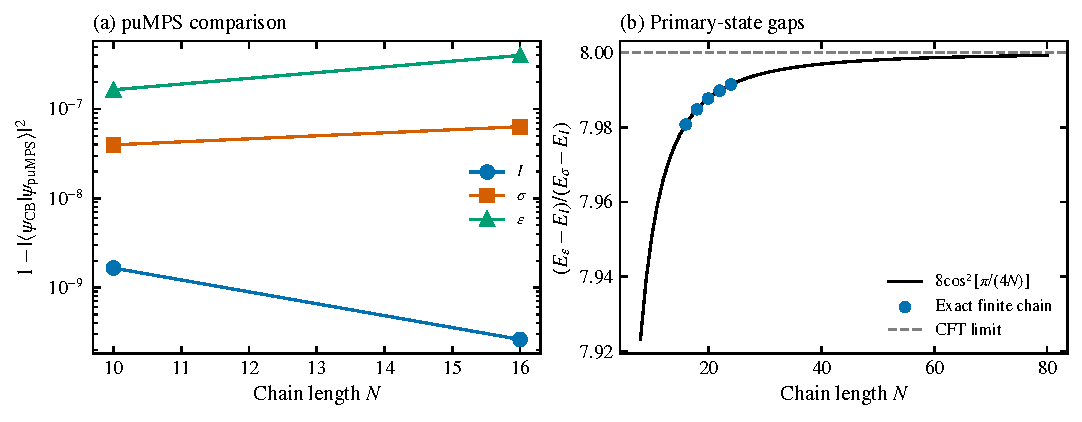
\includegraphics[width=\linewidth]{../figs/state_validation.pdf}
\caption{State validation at critical coupling and periodic spin boundaries.
(a) Squared-overlap infidelities against archived puMPS at
$(N,D_{\rm bond})=(10,8),(16,14)$, seeds $1244,1250$; $\sigma$ uses the
CB-seeded projection with solver tolerance $2\times10^{-12}$.
(b) Exact finite-chain gap ratios at $N=16,18,20,22,24$ and
Eq.~\eqref{eq:gaps}; the dashed line is the continuum value eight.
No interval length or mixture probability enters these whole-state tests.}
\label{fig:validation}
\end{figure}

\clearpage

\subsection{What was checked for the projected spin state}
\label{sec:ising-spin-validation}
For normalized vectors, define the energy error, eigenstate residual,
and squared overlap by
\begin{equation}
 \delta E=|\langle H\rangle-E_\sigma^{\rm exact}|,\qquad
 \eta=\|(H-\langle H\rangle)\ket{\sigma_N}\|_2,\qquad
 F=|\langle\sigma_{\rm ref}|\sigma_N\rangle|^2.
\end{equation}
The residual equals the square root of the energy variance. It tests
closeness to an eigenstate, but does not identify which eigenstate;
parity, translation and the exact lowest odd-sector energy supply that
identification. The interval comparison is
\begin{equation}
 e_\rho=\max_{1\leq\ell\leq\min(5,N/2)}
 \left\|\rho^{\rm Lanczos}_{\sigma,\ell}
       -\rho^{\rm covariance}_{\sigma,\ell}\right\|_F,
 \qquad \|B\|_F=\sqrt{\sum_{u,v}|B_{uv}|^2}.
\end{equation}
The following are the archived results in
\texttt{ising\_cb\_validation.csv}, rounded only for display.
That file evaluates the exact reference energy through the covariance;
using the equivalent trigonometric formula can change the last
roundoff digits of $\delta E$.
\begin{center}\small
\begin{tabular}{rrrrrr}\toprule
$N$ & $F_{\rm seed}$ & $\eta$ & $\delta E$ & $e_\rho$ & $|1-F|$\\\midrule
6 & .985928 & $1.54\,10^{-15}$ & $1.78\,10^{-15}$ & $1.82\,10^{-15}$ & $1.33\,10^{-15}$\\
8 & .982894 & $6.11\,10^{-15}$ & $5.33\,10^{-15}$ & $1.61\,10^{-15}$ & $2.22\,10^{-15}$\\
10 & .980864 & $2.22\,10^{-13}$ & $0$ & $2.76\,10^{-15}$ & $0$\\
12 & .979404 & $1.99\,10^{-11}$ & $2.49\,10^{-14}$ & $2.47\,10^{-13}$ & $1.78\,10^{-15}$\\
16 & .977431 & $2.70\,10^{-12}$ & $4.26\,10^{-14}$ & $4.02\,10^{-14}$ & ---\\\bottomrule
\end{tabular}
\end{center}
Here $F_{\rm seed}=|\langle\sigma_N|q_1\rangle|^2$ measures how much
of the target was already in the seed. For $N\leq12$, $F$ compares
against the lowest three eigenpairs from a separate full-spin-space
Hamiltonian action with a random starting vector. That reference also
uses \texttt{eigsh}; it is a different state construction, not an
independent eigensolver implementation. No full-space overlap was
recorded at $N=16$, hence the dash. Values of $F$ exceeding one by
roundoff are reported as $|1-F|$, not negative infidelities; zero entries
are floating-point results, not proofs of exact arithmetic equality.

The separate \texttt{ising\_construction\_checks.csv} run tests
$|\langle\sigma|\sigma\rangle-1|$,
$\|(P+1)\sigma\|_2$, $\|(\mathsf T-1)\sigma\|_2$, and
$\max_{a=I,\eps}|\langle a|\sigma\rangle|$ on the same five sizes.
Their maxima are $9.99\times10^{-16}$, $0$,
$7.20\times10^{-13}$, and $0$, respectively. Parity and mutual
orthogonality are enforced by disjoint basis sectors, so those zeros
alone do not establish state accuracy.

For context, the archived puMPS $\sigma$ residuals are
$2.65\times10^{-3}$ at $(N,D_{\rm bond})=(10,8)$ and
$3.10\times10^{-3}$ at $(16,14)$. Their squared overlaps with the
reference are $0.9999999603$ and $0.9999999366$.
These comparisons favor the exact reference for this integrable model
and these supplied checkpoints. They do not bound the accuracy of
puMPS after further optimization or at a larger bond dimension.

\subsection{Large-chain contraction and entropy checks}
\label{sec:large-sanity}
Validation tests each link in the calculation, rather than only checking
the final entropy. The 119 larger-interval records are in
\texttt{large\_interval\_checks.csv}; the earlier 345 smaller-interval
checks remain in \texttt{extension\_checks.csv}.
\begin{center}
\begin{minipage}{\linewidth}\small
\captionsetup{type=table}
\begin{tabular}{p{.58\linewidth}rr}\toprule
Check & Count & Largest difference\\\midrule
Boson ten-site matrix versus full wavefunction enumeration,
$N=20$, all three primaries &3&$3.22\times10^{-15}$\\
Boson 100 versus 130 working digits, $N=20,128$, $\ell=10$
&6&$<2\times10^{-14}$\\
Boson partial traces of ten-site matrices versus direct Pfaffians,
$N=20,128$, $\ell=4,5,6,7$ &24&$1.12\times10^{-16}$\\
Ising partial traces versus direct covariance reductions,
$N=32,82,128$, $\ell=4,5,6,7$ &36&$1.23\times10^{-15}$\\
Ising energies versus exact finite-chain formulas,
$N=32,82,128$ &9&$2.85\times10^{-14}$\\
Ising matrix entries between opposite parity sectors, $\ell=10$
&9&$0$\\
Symmetry-block versus full-matrix directed entropy, $\ell=10$
&2&$1.96\times10^{-14}$\\
Entropy threshold $10^{-15}$ versus $10^{-16}$, $\ell=10$
&30&$3.37\times10^{-13}$\\\bottomrule
\end{tabular}
\caption{Large-chain contraction and entropy checks. Counts give
the number of comparisons in each test family; sizes, interval lengths
and primary-state coverage are specified in the first column. Matrix
errors are maximum absolute entrywise differences; energy and entropy
errors are absolute scalar differences. The precision row reports a
validation-tolerance bound on the final double-precision matrices.}
\label{tab:large-validation}
\end{minipage}
\end{center}
Matrix differences in Table~\ref{tab:large-validation} mean the largest absolute entrywise
difference $\max_{u,v}|\rho^{(1)}_{uv}-\rho^{(2)}_{uv}|$; energy and
entropy differences are absolute scalar differences. Precision comparisons
refer to the final complex double-precision matrices, and the displayed
bound is their validation tolerance. The exact zeros refer to the
implemented parity-block structure, not a general error bound.

The full-matrix entropy checks use boson $ss\mid3s,s$ at $N=20$ and
Ising $\sigma\mid\eps$ at $N=82$. The threshold comparison covers all
six directions at $N=20,128$ for the boson and $N=32,82,128$ for Ising.
No mixture is replaced by a covariance-only approximation. The generation
stage independently checks trace, Hermiticity, and minimum eigenvalue for
all 294 state--interval combinations in the requested grid; these records
are in \texttt{large\_interval\_quality.csv}. The 180 observations shared
with the preceding grid retain their original stored values.

The exact contractions remove sampling and variational errors from the
present finite-lattice calculation. They do not remove the physical
dependence on $N$, $\ell$, or the fixed finite endpoint $W=10^8$.
The comparison with CFT in Sec.~\ref{sec:extension} keeps these physical
limitations distinct from numerical contraction accuracy.


Table~\ref{tab:large-validation} lists all eight families of the 119 checks, including
their sizes, norms, and errors. In particular, the $N=20$,
$\ell=10$ boson comparison tests every matrix element of all three
states against full wavefunction enumeration, with maximum error
$3.22\times10^{-15}$. This tests off-diagonal phases as well as
normalization. At $N=128$, where full enumeration is impractical,
increased working precision and agreement between direct and cached
contractions test numerical stability. They share the same algebraic
formula and therefore do not constitute an independent large-$N$
wavefunction proof. The algebra is derived in Sec.~\ref{sec:boson-contraction} and independently
tested at the sizes where enumeration is possible.

For Ising, finite-chain energies, covariance purity, zero-mode parity,
and agreement with smaller full vectors test distinct parts of the
construction. A partial trace of a ten-site matrix is also compared
with reconstruction from the directly restricted covariance. Entropy
checks then compare full-matrix and symmetry-block calculations, and
vary the eigenvalue threshold. Trace, Hermiticity and positivity are
necessary checks; agreement with an independently constructed state
is the stronger check. These tests certify the finite-lattice
calculation at the stated precision, not the absence of continuum
cutoff effects or unknown small-interval corrections.

\subsubsection{Endpoint checks for the extension through \texorpdfstring{$N=256$}{N=256}}
\label{sec:n256-sanity}
Before generating the new sizes, we tested all three states of each CFT
at $N=256$ and $\ell=10$. The 70 records in
\texttt{larger\_size\_checks.csv} test the same contraction in the new
size range. In addition to the matrix and entropy differences defined
in Table~\ref{tab:large-validation}, define
\begin{equation}
 e_G=\max_{r,s}|(G^2+\id)_{rs}|,\qquad
 e_P=|(-1)^N\operatorname{Pf}(G)-P|,\qquad
 e_+=\max(0,-\lambda_{\min}(\rho_A)).
 \label{eq:n256-diagnostics}
\end{equation}
Here $e_G$ tests purity of the full-chain Ising covariance, $e_P$ tests
its parity, and $e_+$ measures a negative eigenvalue caused by numerical
error. The remaining matrix-quality errors are $|\Tr\rho_A-1|$ and
$\max_{u,v}|(\rho_A-\rho_A^\dagger)_{uv}|$.
\begin{center}
\begin{minipage}{\linewidth}\small
\captionsetup{type=table}
\begin{tabular}{p{.61\linewidth}rr}\toprule
Check at $N=256$ & Count & Largest error\\\midrule
Ising exact finite-chain energies &3&$5.69\times10^{-14}$\\
Ising full covariance purity $e_G$ &3&$3.11\times10^{-15}$\\
Ising full-state parity $e_P$ &3&$5.96\times10^{-14}$\\
Ising partial traces versus direct covariance, $\ell=4,6$ &6&$5.42\times10^{-16}$\\
Boson 100 versus 130 digits, $\ell=10$ &3&$<2\times10^{-14}$\\
Boson partial traces versus direct Pfaffians, $\ell=4,6$ &6&$1.39\times10^{-16}$\\
Trace, Hermiticity and $e_+$, both CFTs, $\ell=10$ &18&$2.19\times10^{-16}$\\
Entropy cutoff $10^{-15}$ versus $10^{-16}$, $\ell=4,10$ &24&$7.93\times10^{-14}$\\
Symmetry-block versus full-matrix entropy, $\ell=4,10$ &4&$1.67\times10^{-14}$\\\bottomrule
\end{tabular}
\caption{All 70 endpoint checks for the extension to $N=256$. State
checks cover all three primaries per model; entropy-threshold checks
cover all six directions. Full-matrix comparisons use Ising
$\sigma\mid\eps$ and boson $ss\mid3s,s$. Errors use
Eq.~\eqref{eq:n256-diagnostics} and the entrywise/scalar conventions of
Table~\ref{tab:large-validation}. The precision row gives the validation
tolerance for final complex double-precision matrices, not a claim of
100-digit precision in the returned matrix.}
\label{tab:n256-validation}
\end{minipage}
\end{center}
All checks passed. The additional production run records trace,
Hermiticity and minimum eigenvalue for all $8\times3\times7\times2=336$
new state/interval combinations in \texttt{larger\_size\_quality.csv}.
It appends 672 directed relative entropies while preserving all 1200
earlier observations. The high-precision comparison shares the same
algebra and tests numerical stability; it is not an independent
full-wavefunction check at $N=256$.

\subsection{Reading route and attribution}
\begin{enumerate}
\item \textbf{Ising block states and the spin-primary limitation.}
Read Montes et al.~\cite{Montes2017}, Sec.~VIII, Eqs.~(55)--(62),
for the homogeneous even-sector block and its fermion ground state;
Appendix C, Eqs.~(133)--(137), supplies spin/fermion conventions.
Sec.~X, Eqs.~(73)--(75), constructs the energy-primary endpoint block.
The discussion after Eq.~(79) explains the difficulty with proposed
odd-sector endpoint states. Our summed-spin seed and odd-sector
projection, Eqs.~\eqref{eq:sigmaseed}--\eqref{eq:projection}, are a
project adaptation. They are not a published closed block formula for
$\sigma$.
\item \textbf{Lanczos projection.}
The algorithmic reference is the ARPACK guide~\cite{ARPACK}; the
direct implementation contract is \texttt{eigsh}~\cite{ScipyEigsh}.
The three-term recurrence and Rayleigh--Ritz selection are written out
in Appendix~\ref{sec:sigmamethod}. Our call uses \texttt{k=1},
\texttt{which="SA"}, \texttt{v0=seed}, and \texttt{tol=2e-12}.
It leaves \texttt{ncv} and \texttt{maxiter} at their defaults: for the
tested odd-sector dimension $d=2^{N-1}$, these are $20$ and $10d$.
No shift-invert transformation is requested. The API parameter
\texttt{sigma} denotes a spectral shift and is unrelated to our
primary-state name. The recorded environment uses SciPy 1.17.1;
the linked 1.17-series API describes these parameters.
\item \textbf{Large Ising chains.}
Read Peschel and Eisler~\cite{PeschelEisler}, Sec.~3.3(II),
Eqs.~(14)--(18), including the following Majorana paragraph.
It explains why a subsystem of a quadratic-fermion eigenstate is
determined by restricted correlations. Our explicit parity and zero-mode
selection precedes that reduction. Match the Majorana basis before
matching signs: we use
$\langle a_ra_s\rangle=\delta_{rs}-iG_{rs}$, whereas the review writes
$\delta_{rs}+i\Gamma_{rs}$ and chooses a different sign for one Majorana
per site. After aligning the basis, $G=-\Gamma$.
The Gaussian statement applies to each Ising primary; the mixture in
Eq.~\eqref{eq:large-target} is evaluated as a full matrix.
\item \textbf{Large compact-boson chains.}
Read St\'{e}phan and Pollmann~\cite{Stephan}, Appendix A.1,
Eqs.~(A5)--(A11), for the confluent Vandermonde determinant and
discrete Pfaffian normalization. Appendix A.2, Eqs.~(A14)--(A15),
introduces site weights for diagonal observables. Their site count $L$
and particle count $N$ are our $N$ and $M$. Their diagonal calculation
can discard amplitude phases. Our off-diagonal interval matrix cannot:
Eq.~\eqref{eq:pf-rdm} retains the bra and ket factors explicitly.
The finite-$W$ extension, bordered contraction, tridiagonal solve,
and reuse of repeated minors are developed in Sec.~\ref{sec:boson-contraction}, and are
checked against explicit vertex-state sums.
\item \textbf{Pfaffian signs and numerical evaluation.}
Wimmer~\cite{Wimmer}, Eqs.~(4) and (5), gives the first-row expansion
and congruence identity. These justify the cached recursion and block
elimination used here. Sec.~II A, Eqs.~(15)--(18), explains pivoted
antisymmetric elimination, the basis of our scalar Pfaffian helpers.
Our code implements those elementary updates using NumPy or mpmath;
it does not call the paper's software package. Caching the minors and
sharing multiplicity factors are implementation choices in this project.
\end{enumerate}

\subsection{From a formula to its source function}
All Python paths in this table are relative to
\texttt{src/conformal\_blocks/}; the method functions have source
references in their docstrings. A reduced density matrix is abbreviated
RDM in function and data-file names.
\begin{center}\small
\begin{tabular}{>{\raggedright\arraybackslash}p{.35\linewidth}>{\raggedright\arraybackslash}p{.57\linewidth}}\toprule
Operation & File and functions\\\midrule
Block vacuum and projected $\sigma$
&\path{ising.py}: \path{fusion_blocks}, \path{sigma_from_cb},
\path{hamiltonian_action}, \path{energy_diagnostics}\\
Quadratic sectors, zero modes and Eq.~\eqref{eq:large-ising-rdm}
&\path{ising.py}: \path{majorana_covariance}, \path{pfaffian},
\path{gaussian_rdm}; direct comparison: \path{dense_rdm}\\
Explicit compact-boson amplitudes
&\path{boson.py}: \path{vertex_state}, \path{sector_rdm}\\
Eqs.~\eqref{eq:pf-small} and \eqref{eq:pf-rdm}
&\path{boson_pfaffian.py}: \path{jastrow_rdm},
\path{_tridiagonal_solve}, \path{pfaffian_mp}, \path{_cached_density}\\
Shorter intervals and exact mixture entropy
&\path{boson_pfaffian.py}: \path{block_rdms};
\path{symmetry_entropy.py}: \path{sectors}, \path{directed_entropies}\\
Validation and current-grid generation
&\path{method_sanity.py}, \path{extension_checks.py},
\path{large_interval_checks.py}, \path{large_intervals.py}\\\bottomrule
\end{tabular}
\end{center}

\subsection{A short reproduction run}
From the root of the full reproducibility project, using a Python
environment containing NumPy, SciPy and mpmath, run
\begin{verbatim}
export PYTHONPATH=src
export OPENBLAS_NUM_THREADS=1
python -m conformal_blocks.method_sanity \
  --output method_sanity.json
\end{verbatim}
This script constructs $\sigma$ at $N=12$, checks its energy, residual,
symmetries and four-site reduction, and tests all three primaries at
$N=12,128$ for both CFTs with $\ell=4$. The boson checks compare the
cached 100-digit calculation with direct 130-digit Pfaffians, and at
$N=12$ with explicit vertex amplitudes. It also compares both entropy
implementations. Every check writes its error, tolerance, parameters
and pass flag. The executed result is archived as
\texttt{data/method\_sanity.json}; all 55 checks passed. This compact
reproduction supplements the archived 345 earlier checks and 119
ten-site checks, without replacing them or rerunning any fits.

\clearpage
\section{Relative entropy between primaries}
\label{sec:primary-relative-entropy}
This appendix retains the historical $N\leq256$ sanity-check data,
with fit and display cutoffs $0.08$ and $0.20$, respectively. Its
smallest fraction is $4/256=0.015625$, so it has no observations in
the current mixture display window $x\leq0.01$. Its figures and fits
remain separate from the active mixture analysis in Secs.~\ref{sec:fits}
and \ref{sec:complement}.

This appendix tests the primary interval matrices against a second
observable whose leading coefficient is known analytically. For the same
normalized lattice states used in the mixture study, define
\begin{equation}
 S_{a\Vert b}(N,\ell)
 =S(\rho_A^a\Vert\rho_A^b)
 =\Tr\rho_A^a\log\rho_A^a-\Tr\rho_A^a\log\rho_A^b,
 \qquad x=\ell/N.
 \label{eq:primary-entropy-definition}
\end{equation}
Here $A$ is the interval of $\ell$ sites, and the double bar separates the
first and second density matrices. Both arguments are reductions of
individual primaries; no mixing probability enters this observable.
The global primary vectors may be orthogonal, but the comparison in
Eq.~\eqref{eq:primary-entropy-definition} concerns their local reductions.
Every pair in the main report is tested in both directions. The mixture
data, fitted coefficients, and fitting figures are unchanged.

\subsection{Leading predictions from the supplied literature}
\label{sec:primary-analytic}
The sources are the two S\'{a}rosi--Ugajin papers supplied as
\path{Theory_paper/1603.03057v2.pdf} and
\path{Theory_paper/1611.02959v1.pdf}.
Equations (50) and (53) of the first paper~\cite{Sarosi} give the
leading operator-product-expansion result; its Eq.~(61) gives the stress
tensor contribution, and Eq.~(63) treats free-boson vertex operators.
Equation (1.3) and Secs.~3.1--3.3 of the second
paper~\cite{SarosiHigher} give the corresponding scalar, stress tensor,
and current results. These equation and subsection numbers belong to
the cited source versions. The formulas below specialize those published
results to the states of this report; no unknown subleading coefficient
is derived.

Let $O_j$ be an orthonormal set of the lightest local operators whose
diagonal matrix elements differ in states $a$ and $b$. Their common
scaling dimension is $\Delta$, and
$C_{O_j a^\dagger a}=\langle a|O_j|a\rangle$ denotes the normalized
plane three-point coefficient. The index $j$ labels operators and is
unrelated to the leading exponent $\alpha$. The published result is
\begin{equation}
 S_{a\Vert b}(x)=K(\Delta)
 \sum_j\bigl(C_{O_j a^\dagger a}-C_{O_j b^\dagger b}\bigr)^2
 (\pi x)^{2\Delta}+o(x^{2\Delta}),\qquad
 K(\Delta)=\frac{\Gamma(3/2)\Gamma(\Delta+1)}
 {2\Gamma(\Delta+3/2)}.
 \label{eq:primary-ope}
\end{equation}
The symbol $\Gamma$ denotes Euler's gamma function; $o(x^r)$ means terms
whose ratio to $x^r$ vanishes as $x\to0$ in the continuum theory.
Thus $\alpha=2\Delta$, and $K(1)=1/3$. This leading term is symmetric
under $a\leftrightarrow b$, although the full relative entropy need not
be symmetric. For unequal conformal weights, an operator with
$\Delta<2$ still dominates the stress tensor, as explained immediately
before Eq.~(63) of Ref.~\cite{Sarosi}.

\subsubsection{Ising: identify the first nonzero diagonal difference}
The conformal weights are
$(h_I,\bar h_I)=(0,0)$,
$(h_\sigma,\bar h_\sigma)=(1/16,1/16)$, and
$(h_\eps,\bar h_\eps)=(1/2,1/2)$, with central charge $c=1/2$.
The energy primary $\eps$ has total scaling dimension one; it is the
nonchiral energy field in the periodic spin chain. The Ising fusion
rules $\sigma\times\sigma=I+\eps$ and $\eps\times\eps=I$ imply
that only $\sigma$ has a nonzero diagonal energy-field coefficient.
Using the normalization in Sec.~5 of Ref.~\cite{Sarosi}, the data are
\begin{equation}
 C_{\eps II}=0,\qquad C_{\eps\sigma\sigma}=\tfrac12,
 \qquad C_{\eps\eps\eps}=0.
 \label{eq:primary-ising-ope-data}
\end{equation}
The spin field itself has zero diagonal coefficient
in each of these parity eigenstates, so its smaller scaling dimension
does not produce an $x^{1/4}$ term. Inserting the difference $1/2$
and $K(1)=1/3$ into Eq.~\eqref{eq:primary-ope} gives
\begin{equation}
 S_{I\Vert\sigma}=S_{\sigma\Vert I}
 =S_{\sigma\Vert\eps}=S_{\eps\Vert\sigma}
 =\frac{\pi^2}{12}x^2+o(x^2)
 \quad\text{at leading order}.
 \label{eq:primary-ising-spin}
\end{equation}
The equalities here refer only to the displayed leading term.

For $I\leftrightarrow\eps$, the energy-field diagonal difference
vanishes. The stress tensors $T,\bar T$, of scaling dimension two,
then give the first contribution. Equation (61) of Ref.~\cite{Sarosi}
includes both chiralities for $h=\bar h$:
\begin{equation}
 S_{a\Vert b}(x)=\frac{16}{15c}(h_a-h_b)^2(\pi x)^4+o(x^4).
 \label{eq:primary-stress}
\end{equation}
With $c=1/2$ and $|h_I-h_\eps|=1/2$, this becomes
\begin{equation}
 S_{I\Vert\eps}=S_{\eps\Vert I}
 =\frac{8\pi^4}{15}x^4+o(x^4)
 \quad\text{at leading order}.
 \label{eq:primary-ising-energy}
\end{equation}

\subsubsection{Nonchiral compact boson: add the two current contributions}
Write $\boldsymbol Q_a=(Q_{L,a},Q_{R,a})$ for the left and right
charges, with $h_a=Q_{L,a}^2/2$ and $\bar h_a=Q_{R,a}^2/2$.
The charge convention of Sec.~\ref{sec:bosonconstruction} is
\begin{equation}
 \boldsymbol Q_{00}=(0,0),\qquad
 \boldsymbol Q_{ss}=(s,s),\qquad
 \boldsymbol Q_{3s,s}=(3s,s),\qquad s=1/\sqrt2.
 \label{eq:primary-boson-charges}
\end{equation}
Equation (63) of Ref.~\cite{Sarosi} states the chiral vertex result
$S=(Q_{L,a}-Q_{L,b})^2[1-\pi x\cot(\pi x)]$.
For the leading nonchiral result, use Eq.~\eqref{eq:primary-ope} with
the two orthogonal, dimension-one currents $J_L=i\partial\phi_L$ and
$J_R=i\bar\partial\phi_R$. Their normalized diagonal coefficients
are the corresponding charges, up to the common sign convention
discussed below that source equation. Their squared differences add;
there is no mixed-current contribution because the two currents have
zero two-point overlap. Therefore
\begin{equation}
 S_{a\Vert b}(x)=\frac{\kappa_{ab}\pi^2}{3}x^2+o(x^2),
 \qquad \kappa_{ab}=(Q_{L,a}-Q_{L,b})^2+(Q_{R,a}-Q_{R,b})^2.
 \label{eq:primary-boson-leading}
\end{equation}
The three squared separations are $1$, $5$, and $2$ for
$00\leftrightarrow ss$, $00\leftrightarrow3s,s$, and
$ss\leftrightarrow3s,s$, respectively. The corresponding coefficients
are $\pi^2/3$, $5\pi^2/3$, and $2\pi^2/3$, with $\alpha=2$ in every direction.
This use of both currents also covers the nonzero conformal spin of
$\ket{3s,s}$. It does not apply the spinless stress-tensor formula to
that state.

All coefficients in Eqs.~\eqref{eq:primary-ising-spin},
\eqref{eq:primary-ising-energy}, and \eqref{eq:primary-boson-leading}
are four times the corresponding equal-mixture leading coefficients in
Sec.~\ref{sec:coefficients}. This agreement follows by comparing the
published leading formulas. The numerical values below are computed
directly from Eq.~\eqref{eq:primary-entropy-definition}, rather than
obtained by multiplying the mixture data by four.

\subsection{Direct numerical procedure and checks}
\label{sec:primary-numerics}
The calculation uses every geometry displayed in the main report:
the 15 sizes in Eq.~\eqref{eq:large-grid}, $\ell=6,\ldots,10$, and
$x\leq0.20$. This gives 70 observations for each of 12 directions,
or 840 displayed direct primary relative entropies. The 51 points per direction
with $x\leq0.08$ define the analytical CFT comparison window.
Section~\ref{sec:primary-fits} subsequently fits the same numerical
data; those fits do not enter this leading-theory comparison.
\begin{enumerate}
\item Load the existing $\ell=10$ primary density matrices and obtain
shorter intervals by the partial trace of Sec.~\ref{sec:extension}.
Ising uses exact Jordan--Wigner states for all three primaries. The
boson uses the same normalized finite-$W$ vertex/Jastrow states with
$q=2$, unit-circle sites, $w_1=0$, $W=10^8$, and 100 decimal working
digits in their Pfaffian construction. No new primary optimization is
performed.
\item Diagonalize each local parity block (Ising) or occupation block
(boson), retaining its original trace. Denote target eigenvectors by
$|v_{bj}\rangle$, target eigenvalues by $\lambda_{bj}$, and the
first state's weights in that basis by
$w_{aj}^{(b)}=\langle v_{bj}|\rho_A^a|v_{bj}\rangle$.
The index $j$ runs over eigenvectors in all blocks. The matrices need
not commute; their eigenvectors are essential in this cross term.
\item Evaluate the spectral trace with natural logarithms:
\begin{equation}
 S^{(\tau)}_{a\Vert b}
 =\sum_{\lambda_{aj}>0}\lambda_{aj}\log\lambda_{aj}
 -\sum_j w_{aj}^{(b)}\log\!\bigl[\max(\lambda_{bj},\tau)\bigr],
 \qquad \tau=10^{-15}.
 \label{eq:primary-numerical-trace}
\end{equation}
The small eigenvalue floor $\tau$ only regularizes the target logarithm;
it does not renormalize or flatten a symmetry block. Negative
eigenvalues at roundoff scale are omitted from the self-entropy sum;
an eigenvalue below $-2\times10^{-12}$ aborts the calculation.
\item Check the regularization by repeating the logarithms at
$\tau=10^{-14}$ and $10^{-16}$. Record both the span of the three
entropy values and the first-state weight on target modes below the
production floor,
\begin{equation}
 t_{a\Vert b}=\sum_{\lambda_{bj}<10^{-15}}
 \max(w_{aj}^{(b)},0).
 \label{eq:primary-tail}
\end{equation}
An exact target null space with nonzero first-state weight would make
the unregularized relative entropy infinite. The floor is consequently
audited, rather than used to conceal a support mismatch. Cutoff
sensitivity is a numerical stability test, not a rigorous bound on
unresolved eigenvalues.
\end{enumerate}

There are 4824 passing numerical checks. The maximum entropy span over
the three floors is $1.66\times10^{-10}$, below the
$2\times10^{-10}$ tolerance; the maximum $t_{a\Vert b}$ is
$1.50\times10^{-11}$, below $2\times10^{-11}$.
All directed values are nonnegative, and self-comparisons
$S^{(\tau)}_{a\Vert a}$ have maximum absolute magnitude
$3.23\times10^{-13}$ over all three floors.
At $N=256$, $\ell=4,6$, direct diagonalization of the full interval
matrix agrees with the symmetry-block calculation for all pairs to
$4.67\times10^{-15}$.

For every Ising geometry we also check a formula that operates on the
$2\ell\times2\ell$ one-particle matrices instead of the
$2^\ell\times2^\ell$ many-body matrices. Define
$C_a=(\mathbb I+i\Gamma_{a,A})/2$, where $\Gamma_{a,A}$ is the
restricted Majorana covariance defined in Sec.~\ref{sec:large-ising}.
Gaussian mode decomposition~\cite{PeschelEisler} gives
\begin{equation}
 S_{a\Vert b}=\operatorname{tr}_{2\ell}
 \bigl[C_a(\log C_a-\log C_b)\bigr].
 \label{eq:primary-gaussian-check}
\end{equation}
In this doubled Majorana representation, the eigenvalues occur as
$n_j,1-n_j$; both occupations of each fermionic mode are already counted,
so no extra factor of $1/2$ is inserted. In the eigenbasis of $C_b$,
the quadratic target logarithm is averaged using the diagonal weights
of $C_a$, which yields the cross term in
Eq.~\eqref{eq:primary-gaussian-check}. This independent evaluation
agrees with the many-body trace to $2.35\times10^{-12}$ across all
600 Ising directed comparisons. These checks validate the entropy
evaluation; they do not remove the physical finite-interval corrections.

\subsection{Comparison with the analytical CFT leading term}
\label{sec:primary-results}
Let $B_{ab}$ denote the analytical coefficient obtained above, and define
\begin{align}
 S^{\rm LO}_{a\Vert b}(x)&=B_{ab}x^\alpha,
 &R_{a\Vert b}&=\frac{S_{a\Vert b}}{S^{\rm LO}_{a\Vert b}},\notag\\
 \delta_{a\Vert b}[\%]&=100(R_{a\Vert b}-1),
 &E_m[\%]&=\sqrt{\frac1m\sum_{i:x_i\leq0.08}\delta_i^2}.
 \label{eq:primary-comparison-metrics}
\end{align}
LO means leading order. The denominator in the percentage is the
analytical prediction. The index $i$ runs over the $m=51$ geometries for
one direction. Neither $B_{ab}$ nor $\alpha$ is fitted.
Tables~\ref{tab:ising-primary-entropy} and
\ref{tab:boson-primary-entropy} show every directed pair, while
Fig.~\ref{fig:primary-entropy-leading} shows the interval dependence.

\begin{table}[htbp]\centering\scriptsize
\begin{tabular}{lrrrrrrr}\toprule
Direction & $\alpha$ & $B_{ab}$ & $S_{10}$ & $S_{10}^{\rm LO}$ & $\delta_6$ (\%) & $\delta_{10}$ (\%) & $E_m$ (\%)\\\midrule
$I\Vert \sigma$ & 2 & $(1/12)\pi^{2}$ & 0.0012566 & 0.001255 & +0.106 & +0.126 & 0.221\\
$\sigma\Vert I$ & 2 & $(1/12)\pi^{2}$ & 0.0012566 & 0.001255 & +0.117 & +0.130 & 0.232\\
$I\Vert \varepsilon$ & 4 & $(8/15)\pi^{4}$ & $1.16\!\times\!10^{-4}$ & $1.21\!\times\!10^{-4}$ & -2.854 & -4.439 & 7.160\\
$\varepsilon\Vert I$ & 4 & $(8/15)\pi^{4}$ & $1.18\!\times\!10^{-4}$ & $1.21\!\times\!10^{-4}$ & -2.079 & -2.388 & 3.940\\
$\sigma\Vert \varepsilon$ & 2 & $(1/12)\pi^{2}$ & 0.001342 & 0.001255 & +2.437 & +6.932 & 11.634\\
$\varepsilon\Vert \sigma$ & 2 & $(1/12)\pi^{2}$ & 0.0013738 & 0.001255 & +3.313 & +9.469 & 16.494\\
\bottomrule\end{tabular}

\caption{Ising primary relative entropy sanity check for all six
directions under the critical periodic Hamiltonian
$H=-\sum XX-\sum Z$. The theoretical coefficient $B_{ab}$ multiplies
$x^\alpha$, including its power of $\pi$. Here $S_{10}$ and $S_{10}^{\rm LO}$ are respectively
the direct numerical entropy and its analytical CFT leading-order prediction at
$N=256$, $\ell=10$, $x=5/128$; both use natural logarithms.
$\delta_6$ and $\delta_{10}$ are signed deviations at $N=256$ for
$\ell=6$ and ten, respectively. $E_m$ uses all $m=51$ geometries with
$x\leq0.08$ and is defined by Eq.~\eqref{eq:primary-comparison-metrics}.
All primaries and spectral checks are specified in
Sec.~\ref{sec:primary-numerics}; every coefficient is fixed analytically.}
\label{tab:ising-primary-entropy}
\end{table}
\begin{table}[htbp]\centering\scriptsize
\begin{tabular}{lrrrrrrr}\toprule
Direction & $\alpha$ & $B_{ab}$ & $S_{10}$ & $S_{10}^{\rm LO}$ & $\delta_6$ (\%) & $\delta_{10}$ (\%) & $E_m$ (\%)\\\midrule
$00\Vert ss$ & 2 & $(1/3)\pi^{2}$ & 0.0048262 & 0.0050199 & -6.829 & -3.859 & 5.291\\
$ss\Vert 00$ & 2 & $(1/3)\pi^{2}$ & 0.0048262 & 0.0050199 & -6.830 & -3.860 & 5.293\\
$00\Vert 3s,s$ & 2 & $(5/3)\pi^{2}$ & 0.024469 & 0.0251 & -4.780 & -2.515 & 3.579\\
$3s,s\Vert 00$ & 2 & $(5/3)\pi^{2}$ & 0.024466 & 0.0251 & -4.792 & -2.527 & 3.615\\
$ss\Vert 3s,s$ & 2 & $(2/3)\pi^{2}$ & 0.0099902 & 0.01004 & -1.702 & -0.495 & 1.035\\
$3s,s\Vert ss$ & 2 & $(2/3)\pi^{2}$ & 0.0099884 & 0.01004 & -1.721 & -0.513 & 1.084\\
\bottomrule\end{tabular}

\caption{Compact-boson primary relative entropy for all six directions,
with the same geometry and indicator definitions as
Table~\ref{tab:ising-primary-entropy}. The normalized vertex/Jastrow
states have charges in Eq.~\eqref{eq:primary-boson-charges}, $q=2$,
$z_j=e^{2\pi i j/N}$, $w_1=0$, $W=10^8$, and no orthogonalization.
All rows have fixed $\alpha=2$; $B_{ab}=\kappa_{ab}\pi^2/3$ follows from
Eq.~\eqref{eq:primary-boson-leading}. The data use the primary target
$\rho_A^b$, with no mixture.}
\label{tab:boson-primary-entropy}
\end{table}

At $N=256$, $\ell=10$, the Ising $I\leftrightarrow\sigma$ deviations
are about $+0.13\%$. The $I\Vert\eps$ and $\eps\Vert I$ deviations
are $-4.44\%$ and $-2.39\%$, whereas
$\sigma\Vert\eps$ and $\eps\Vert\sigma$ give $+6.93\%$ and
$+9.47\%$. Reducing $x$ to $3/128$ with $\ell=6$ reduces the latter
two deviations to $+2.437\%$ and $+3.313\%$, while also changing the
lattice resolution. In the boson, the largest absolute deviation at
$N=256$, $\ell=10$ is $3.86\%$, and the
$ss\leftrightarrow3s,s$ deviations are about $-0.5\%$.

The leading predictions thus reproduce the scales and small-$x$
behavior across the pairs, with the residual deviations explicitly
resolved. The $\sigma\leftrightarrow\eps$ channels are particularly
sensitive to retaining only their leading term: over the entire
$x\leq0.08$ window their maximum signed deviations reach $24.9\%$
and $36.1\%$. Smaller $x$ at fixed $\ell$ and larger $\ell$ in lattice
units address different limits, as discussed in
Sec.~\ref{sec:large-scales}. This sanity check is not a controlled
continuum extrapolation or an assertion that a leading-only expression
is exact on the finite-chain grid.

The implementation is \path{src/conformal_blocks/primary_relative_entropy.py}.
The raw \path{primary_relative_entropy.csv} retains all 1200 observations, including excluded lengths. The selection module rebuilds
\path{primary_entropy_summary.csv} (12 directional summaries),
\path{primary_entropy_checks.csv} (4824 numerical checks), and
\path{primary_entropy_validation.json} in the report's data directory.
The independent renderer \path{report/primary_entropy_artifacts.py}
reads these CSVs. From the project root, the reproducible commands are
\begin{verbatim}
PYTHONPATH=src $PY -m conformal_blocks.primary_selection
MPLCONFIGDIR=/tmp/relative_entropy_mpl $PY report/primary_entropy_artifacts.py
\end{verbatim}
Here \texttt{\$PY} is the approved Python interpreter specified in the
reproduction instructions, with one BLAS thread. Existing cached density
matrices are reused; if absent, the same production formulas recompute them.

\begin{figure}[p]\centering
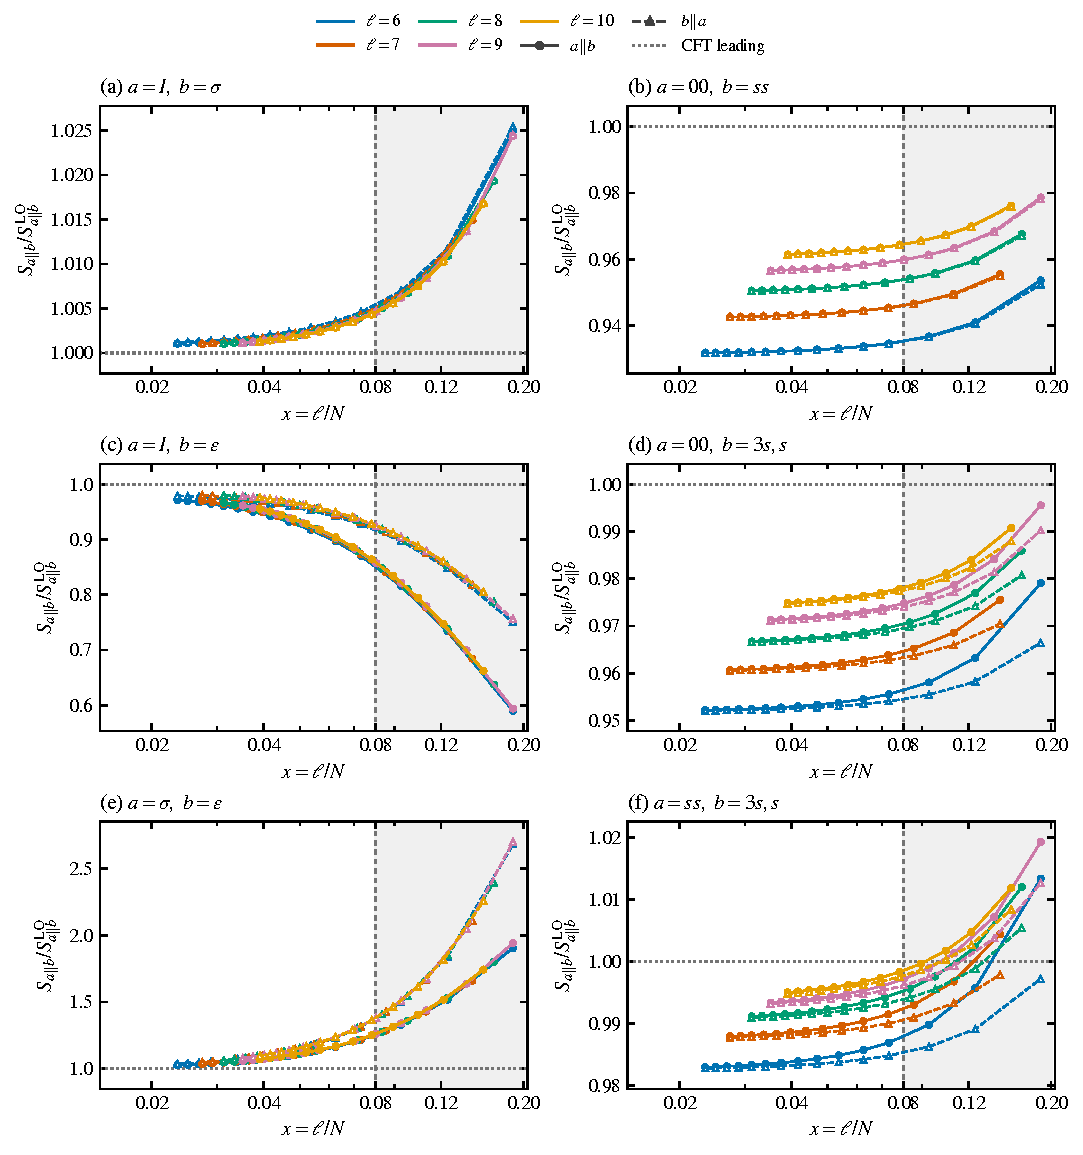
\includegraphics[width=.95\linewidth]{../figs/primary_entropy_leading.pdf}
\caption{Historical parameter-free leading-order check of primary relative entropy.
Each panel compares the two directions between the states $a,b$ named
in its title; the left column is Ising and the right column the compact
boson. The ordinate is $R=S_{a\Vert b}/[B_{ab}x^\alpha]$,
defined by Eq.~\eqref{eq:primary-comparison-metrics}; the dotted line
at one is the analytical CFT leading-order prediction. Colors identify
$\ell=6,\ldots,10$. Solid lines with filled circles denote $a\Vert b$,
and dashed lines with open triangles denote $b\Vert a$; segments only
connect computed sizes. Each direction has 70 points from the 15 sizes
through $N=256$ in Eq.~\eqref{eq:large-grid}, displayed for
$x\leq0.20$. The vertical line at $x=0.08$ marks the 51-point summary
window; shaded points are outside that window. There are no fitted
curves or optimized parameters. Ising uses exact Jordan--Wigner
primaries of $H=-\sum XX-\sum Z$ with periodic spins; the boson uses
the charges and $q=2$, $W=10^8$ construction in
Table~\ref{tab:boson-primary-entropy}. All logarithms are natural,
and the audited target-logarithm floor is $10^{-15}$.
$\alpha=4$, $B=8\pi^4/15$ for Ising $I\leftrightarrow\eps$;
$\alpha=2$, $B=\pi^2/12$ for the other Ising panels;
$\alpha=2$, $B=\pi^2/3,5\pi^2/3,2\pi^2/3$ for the boson panels from top to bottom.
Differences between reverse directions and departures from one remain
visible; the analytical equality is a leading-order statement.}
\label{fig:primary-entropy-leading}
\end{figure}
\clearpage
\subsection{Free power-law fits for the primary pairs}
\label{sec:primary-fits}
To test whether the numerical primary relative entropies recover both
parts of the analytical leading term, we fit one power law with a
free coefficient and a free exponent. The six-panel presentation follows
Figs.~\ref{fig:isingfits}--\ref{fig:bosonresid}; the fitting model below
is specific to the primary-pair comparison. The parameter-free checks
in Secs.~\ref{sec:primary-analytic}--\ref{sec:primary-results} remain
independent of these fits.

For a fixed directed pair $a\Vert b$, let $y_i=S_{a\Vert b}(x_i)$
denote a numerical observation. Define the fitted model and the
analytical leading prediction by
\begin{align}
 F(x;C,\alpha)&=Cx^\alpha,\qquad
 F_{\rm CFT}(x)=B_{ab}x^{\alpha_{\rm CFT}}, \notag\\
 (\widehat C,\widehat\alpha)
 &=\mathop{\mathrm{arg\,min}}_{C>0,\ \alpha\in\mathbb R}
   \sum_{i:x_i\leq0.08}\bigl[y_i-Cx_i^\alpha\bigr]^2 .
 \label{eq:primary-fit-ansatz}
\end{align}
Both $C$ and $\alpha$ are optimized, giving two free parameters.
No theoretical exponent or coefficient is supplied to the optimizer,
and the exponent is not restricted to an integer or to a neighborhood
of its CFT value. Positivity of $C$ enforces a positive power-law
entropy. This is unweighted nonlinear least squares in the entropy
itself; the logarithmic axes do not change the objective.
The analytical values $B_{ab}$ and $\alpha_{\rm CFT}$ from
Sec.~\ref{sec:primary-analytic} are used only for the subsequent
comparison. The CFT prediction has zero free parameters.

For a reproducible numerical procedure, set $x_\star=0.08$ and write
\begin{equation}
 t_i=\ln(x_i/x_\star),\quad
 F(x_i)=\exp(u+\alpha t_i),\quad
 C=\exp(u)x_\star^{-\alpha}.
 \label{eq:primary-free-pivot}
\end{equation}
First regress $\ln y_i$ on $t_i$ to obtain a data-based starting
guess for $(u,\alpha)$. Then optimize both variables against the
original entropies using Eq.~\eqref{eq:primary-fit-ansatz}.
The log-data regression supplies only an initial guess.
The solver uses derivatives
$\partial_uF=F$ and $\partial_\alpha F=Ft_i$;
rescaling all residuals by their common entropy scale does not
change the minimum. Finally convert the fitted amplitude to
$\widehat C$ using Eq.~\eqref{eq:primary-free-pivot}.

The fit uses 51 observations per direction from 12 contributing
system sizes, with the selection $\ell=6,\ldots,10$ and $x\leq0.08$.
The figures show 70 observations per direction from all 15 sizes
in Eq.~\eqref{eq:large-grid}, with $\ell=6,\ldots,10$ and $x\leq0.20$.
The 19 displayed observations outside $x\leq0.08$ do not affect any
coefficient or table metric. Curves beyond the vertical cutoff are
extrapolations of the fitted power law.

For clarity, define the signed entropy residual $r_i$, its percentage
$\eta_i$, and the root mean square error (RMSE), for either
$M=F$ or $M=F_{\rm CFT}$, by
\begin{equation}
 r_i=y_i-M(x_i),\qquad
 \eta_i=100\,\frac{r_i}{y_i},\qquad
 {\rm RMSE}_M=\sqrt{\frac{1}{51}\sum_{i:x_i\leq0.08}r_i^2}.
 \label{eq:primary-fit-residual}
\end{equation}
The percentage denominator here is the numerical entropy $y_i$.
It differs from the analytical denominator in
Eq.~\eqref{eq:primary-comparison-metrics}.
The two signed parameter deviations are
\begin{equation}
 \delta C[\%]=100\left(\frac{\widehat C}{B_{ab}}-1\right),
 \qquad
 \delta\alpha[\%]=100\left(
       \frac{\widehat\alpha}{\alpha_{\rm CFT}}-1\right).
 \label{eq:primary-parameter-errors}
\end{equation}
The coefficient comparison uses powers of $x$ itself, including all powers of $\pi$.
The archived amplitude $\widetilde C$ multiplying $(\pi x)^\alpha$
is converted by $C=\pi^\alpha\widetilde C$.
Changing this convention changes coefficient comparisons when the
exponents differ, so the convention must accompany the numbers.

Cross-validation (CV) omits one of the 12 contributing sizes,
refits \emph{both} parameters on the other 11, and predicts all
omitted observations. If $F^{(-N_i)}$ is the resulting prediction
for observation $i$, define
\begin{equation}
 {\rm CVRMSE}=\sqrt{\frac1{51}\sum_{i:x_i\leq0.08}
       [y_i-F^{(-N_i)}(x_i)]^2}.
 \label{eq:primary-free-cv}
\end{equation}
The residual degrees of freedom are $51-2=49$ for the free fit
and 51 for the analytical CFT leading-order prediction.
For the latter, CV RMSE equals RMSE because no parameter is refitted.

Tables~\ref{tab:ising-primary-all-fits}--\ref{tab:boson-primary-all-fits}
compare both fitted parameters with their analytical values.
For Ising, in the ordered-pair order of Table~\ref{tab:ising-primary-all-fits}, the fitted exponents are $2.0040, 2.0041, 3.8376, 3.9196, 2.2160, 2.3071$.
The boson exponents lie between $2.0050$ and $2.0090$.
The Ising spin--energy coefficients are $1.75660, 2.40358$, compared with $B_{ab}=\pi^2/12$.
A two-parameter power law over a finite window estimates an effective
coefficient and exponent; agreement of its curve with the data
does not by itself establish their asymptotic CFT values.
No additional term or lattice-correction model enters this fit.

\subsubsection{Complete Ising fitting table}
\label{sec:primary-ising-fit-table}
{\footnotesize\setlength{\tabcolsep}{3pt}\renewcommand{\arraystretch}{1.15}
\begin{longtable}{lrrrrrrrrr}
\caption{Ising primary-pair free power-law fits, $F(x)=\widehat Cx^{\widehat\alpha}$: both $C$ and $\alpha$ are optimized on 51 samples per direction, with $\ell=6,\ldots,10$, at $x\leq0.08$. The analytical CFT leading-order prediction is $B_{ab}x^{\alpha_{\rm CFT}}$, with no fitted parameters. All amplitudes include their powers of $\pi$. Parameter deviations use Eq.~\eqref{eq:primary-parameter-errors}; RMSE and CV RMSE refer to the free fit, and CFT RMSE to this analytical CFT prediction. Natural logarithms and the complete definitions in Sec.~\ref{sec:primary-fits} apply.}
\label{tab:ising-primary-all-fits}\\\toprule
Direction & $B_{ab}$ & $\widehat C$ & $\delta C$ [\%] & $\alpha_{\rm CFT}$ & $\widehat\alpha$ & $\delta\alpha$ [\%] & RMSE & CFT RMSE & CV RMSE\\\midrule\endfirsthead
\toprule
Direction & $B_{ab}$ & $\widehat C$ & $\delta C$ [\%] & $\alpha_{\rm CFT}$ & $\widehat\alpha$ & $\delta\alpha$ [\%] & RMSE & CFT RMSE & CV RMSE\\\midrule\endhead
\bottomrule\endfoot
$I\Vert \sigma$ & $1\pi^{2}/12$ & 0.8344 & 1.4505 & 2 & 2.004 & 0.20221 & $6.54\!\times\!10^{-7}$ & $7.21\!\times\!10^{-6}$ & $7.06\!\times\!10^{-7}$\\
$\sigma\Vert I$ & $1\pi^{2}/12$ & 0.83465 & 1.4819 & 2 & 2.0041 & 0.20553 & $7.67\!\times\!10^{-7}$ & $7.50\!\times\!10^{-6}$ & $8.33\!\times\!10^{-7}$\\
$I\Vert \varepsilon$ & $8\pi^{4}/15$ & 29.732 & -42.77 & 4 & 3.8376 & -4.059 & $2.44\!\times\!10^{-6}$ & $7.02\!\times\!10^{-5}$ & $2.64\!\times\!10^{-6}$\\
$\varepsilon\Vert I$ & $8\pi^{4}/15$ & 39.286 & -24.38 & 4 & 3.9196 & -2.01 & $1.95\!\times\!10^{-6}$ & $3.76\!\times\!10^{-5}$ & $2.23\!\times\!10^{-6}$\\
$\sigma\Vert \varepsilon$ & $1\pi^{2}/12$ & 1.7566 & 113.58 & 2 & 2.216 & 10.802 & $2.40\!\times\!10^{-5}$ & $3.95\!\times\!10^{-4}$ & $2.76\!\times\!10^{-5}$\\
$\varepsilon\Vert \sigma$ & $1\pi^{2}/12$ & 2.4036 & 192.24 & 2 & 2.3071 & 15.353 & $3.60\!\times\!10^{-5}$ & $5.66\!\times\!10^{-4}$ & $4.10\!\times\!10^{-5}$\\
\end{longtable}

}

\subsubsection{Complete compact-boson fitting table}
\label{sec:primary-boson-fit-table}
{\footnotesize\setlength{\tabcolsep}{3pt}\renewcommand{\arraystretch}{1.15}
\begin{longtable}{lrrrrrrrrr}
\caption{Compact-boson primary-pair free power-law fits, $F(x)=\widehat Cx^{\widehat\alpha}$: both $C$ and $\alpha$ are optimized on 51 samples per direction, with $\ell=6,\ldots,10$, at $x\leq0.08$. The analytical CFT leading-order prediction is $B_{ab}x^{\alpha_{\rm CFT}}$, with no fitted parameters. All amplitudes include their powers of $\pi$. Parameter deviations use Eq.~\eqref{eq:primary-parameter-errors}; RMSE and CV RMSE refer to the free fit, and CFT RMSE to this analytical CFT prediction. Natural logarithms and the complete definitions in Sec.~\ref{sec:primary-fits} apply.}
\label{tab:boson-primary-all-fits}\\\toprule
Direction & $B_{ab}$ & $\widehat C$ & $\delta C$ [\%] & $\alpha_{\rm CFT}$ & $\widehat\alpha$ & $\delta\alpha$ [\%] & RMSE & CFT RMSE & CV RMSE\\\midrule\endfirsthead
\toprule
Direction & $B_{ab}$ & $\widehat C$ & $\delta C$ [\%] & $\alpha_{\rm CFT}$ & $\widehat\alpha$ & $\delta\alpha$ [\%] & RMSE & CFT RMSE & CV RMSE\\\midrule\endhead
\bottomrule\endfoot
$00\Vert ss$ & $1\pi^{2}/3$ & 3.2114 & -2.3851 & 2 & 2.009 & 0.44964 & $9.35\!\times\!10^{-5}$ & $4.46\!\times\!10^{-4}$ & $1.07\!\times\!10^{-4}$\\
$ss\Vert 00$ & $1\pi^{2}/3$ & 3.2106 & -2.4094 & 2 & 2.0089 & 0.44594 & $9.36\!\times\!10^{-5}$ & $4.47\!\times\!10^{-4}$ & $1.07\!\times\!10^{-4}$\\
$00\Vert 3s,s$ & $5\pi^{2}/3$ & 16.286 & -0.99214 & 2 & 2.0079 & 0.39731 & $3.50\!\times\!10^{-4}$ & 0.0014811 & $4.02\!\times\!10^{-4}$\\
$3s,s\Vert 00$ & $5\pi^{2}/3$ & 16.231 & -1.3301 & 2 & 2.007 & 0.34759 & $3.62\!\times\!10^{-4}$ & 0.0015101 & $4.16\!\times\!10^{-4}$\\
$ss\Vert 3s,s$ & $2\pi^{2}/3$ & 6.6504 & 1.0737 & 2 & 2.0063 & 0.31743 & $7.02\!\times\!10^{-5}$ & $1.49\!\times\!10^{-4}$ & $8.04\!\times\!10^{-5}$\\
$3s,s\Vert ss$ & $2\pi^{2}/3$ & 6.6204 & 0.61876 & 2 & 2.005 & 0.25236 & $7.70\!\times\!10^{-5}$ & $1.65\!\times\!10^{-4}$ & $8.85\!\times\!10^{-5}$\\
\end{longtable}

}

\clearpage
\subsubsection{Reproducing the primary fits}
The command module \path{src/conformal_blocks/primary_fits.py} calls
\path{primary_powerlaw.py} on the existing direct measurements
in \path{primary_relative_entropy.csv}; no density matrix is recomputed.
Its separate outputs in \path{report/data/} are
\path{primary_fit_summary.csv} (24 free/CFT summaries),
\path{primary_fit_input.csv} (612 selected observations),
\path{primary_fit_residuals.csv} (1224 selected residuals),
\path{primary_display_input.csv} (840 displayed observations),
\path{primary_display_predictions.csv} (1680 displayed predictions),
\path{primary_exact_coefficients.csv} (12 analytical leading terms),
and \path{primary_free_power_cv.csv} (144 omitted-size refits).
The public entropy column is \path{S_primary}.
The full summary CSV retains both parameter estimates and deviations,
squared-error sums, relative-residual indicators from Eq.~\eqref{eq:metrics},
and the minimum and maximum of both parameters across the 12 CV fits.
Its additional local diagnostics use the Jacobian
$J_{i1}=F_i$, $J_{i2}=F_it_i$ in variables $(u,\alpha)$:
$\kappa_J=\sigma_{\max}(J)/\sigma_{\min}(J)$ and the covariance
$({\rm SSE}/49)(J^TJ)^{-1}$. Transforming this covariance to
$(C,\alpha)$ gives a matrix $V$. The exported standard errors are
$\sqrt{V_{11}}$ and $\sqrt{V_{22}}$, and the parameter correlation
is $V_{12}/\sqrt{V_{11}V_{22}}$.
These local linearization diagnostics are descriptive, not confidence
intervals for correlated lattice data.

The archived solver CSV uses its original $(\pi x)^\alpha$ amplitude.
The report converter writes \path{primary_reported_coefficients.csv}
with $C=\pi^{\widehat\alpha}\widetilde C$ and
$B_{ab}=\pi^{\alpha_{\rm CFT}}\widetilde B_{ab}$, including the
transformed coefficient errors and local covariance. Physical curves,
exponents and residuals are invariant under this conversion.

An independent check eliminates the amplitude at each trial exponent:
\begin{equation}
 \widehat A(\alpha)=
  \frac{\sum_i y_i v_i(\alpha)}{\sum_i v_i(\alpha)^2},
 \qquad v_i(\alpha)=(x_i/x_\star)^\alpha .
 \label{eq:primary-profile-check}
\end{equation}
Minimizing the remaining one-dimensional objective independently checks
the two-parameter solver. This check covers all 12 complete fits
and all 144 omitted-size fits; a synthetic power law with the
noninteger exponent $2.37$ also verifies that the solver recovers
a free exponent. The implementation is
\path{report/primary_free_fit_checks.py}.
With the interpreter variable \path{PY} defined in
Sec.~\ref{sec:primary-results}, run from the project root:
\begin{verbatim}
PYTHONPATH=src $PY -m conformal_blocks.primary_fits
PYTHONPATH=src MPLCONFIGDIR=/tmp/relative_entropy_mpl \
  $PY report/primary_fit_artifacts.py
PYTHONPATH=src $PY report/primary_free_fit_checks.py
\end{verbatim}
The renderer reads these CSVs to generate the four vector PDF figures
and Tables~\ref{tab:ising-primary-all-fits}--\ref{tab:boson-primary-all-fits}.

\clearpage
\begin{figure}[p]\centering
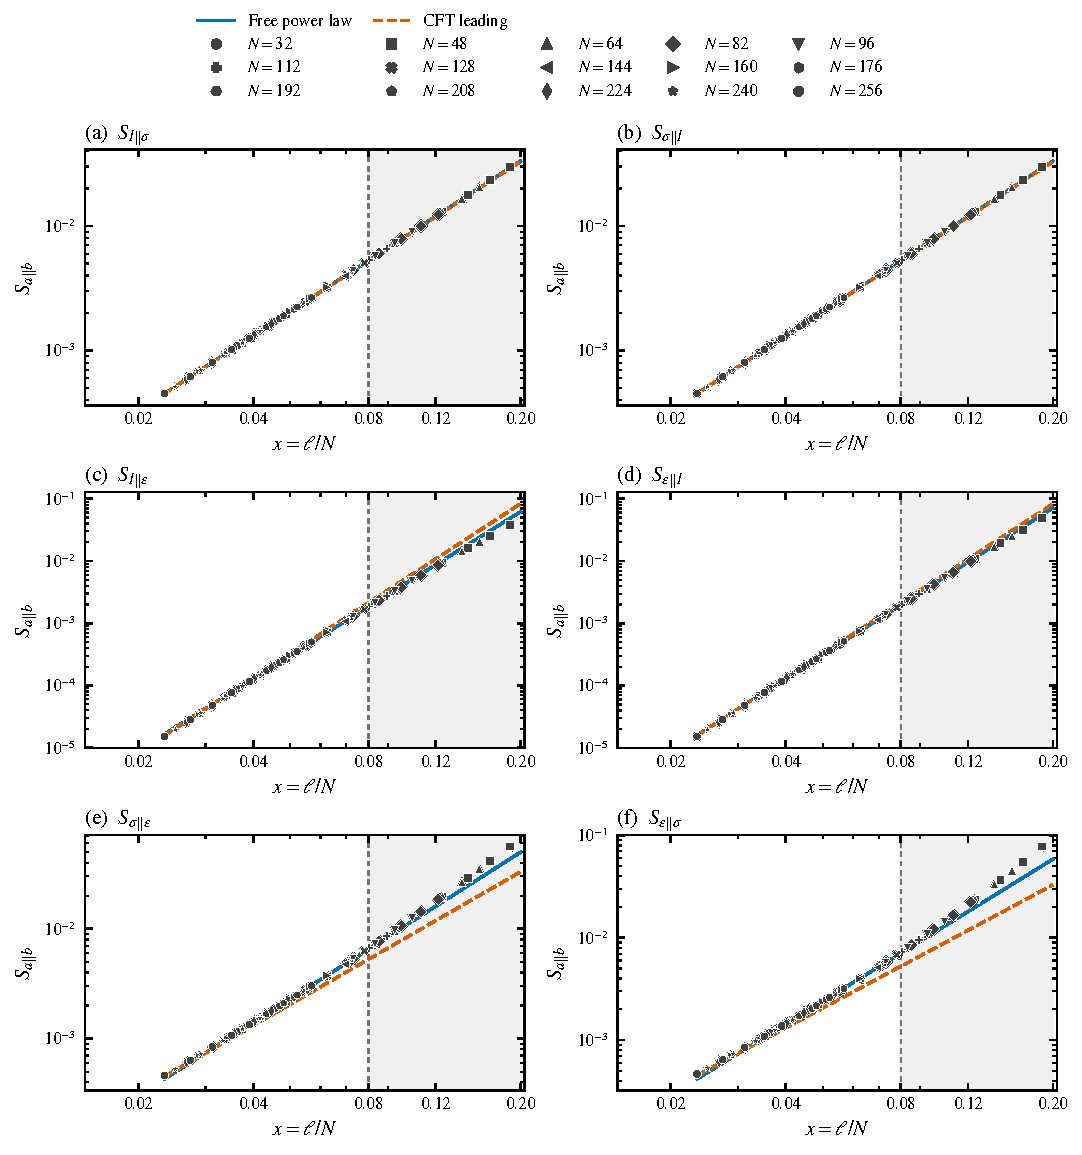
\includegraphics[width=.95\linewidth]{../figs/ising_primary_fits.pdf}
\caption{Historical Ising primary relative entropy $S_{a\Vert b}$ for
all six directions. Markers identify the 15 system sizes through
$N=256$ in Eq.~\eqref{eq:large-grid}; $\ell=6,\ldots,10$.
Each panel shows 70 observations with $x=\ell/N\leq0.20$.
Only the 51 observations at $x\leq0.08$ enter the unweighted
least-squares fits in Eq.~\eqref{eq:primary-fit-ansatz}.
The vertical line and shading mark the cutoff and the extrapolation
region containing 19 observations. Blue solid lines show the free
power law $F=\widehat Cx^{\widehat\alpha}$; both parameters
are optimized independently for each direction. Orange dashed
lines show the analytical CFT leading-order prediction, with no fitted parameters. For panels (c,d),
$\alpha_{\rm CFT}=4$ and $B_{ab}=8\pi^4/15$; elsewhere
$\alpha_{\rm CFT}=2$ and $B_{ab}=\pi^2/12$.
Table~\ref{tab:ising-primary-all-fits} compares both fitted
parameters with these analytical values.
The data use exact Jordan--Wigner primaries of the critical
periodic-spin Hamiltonian $H=-\sum XX-\sum Z$,
natural logarithms, and target-logarithm floor $10^{-15}$.
Both axes are logarithmic. The fitted exponent is a free real
number and the coefficient is positive; no additional powers enter.}
\label{fig:ising-primary-fits}
\end{figure}

\begin{figure}[p]\centering
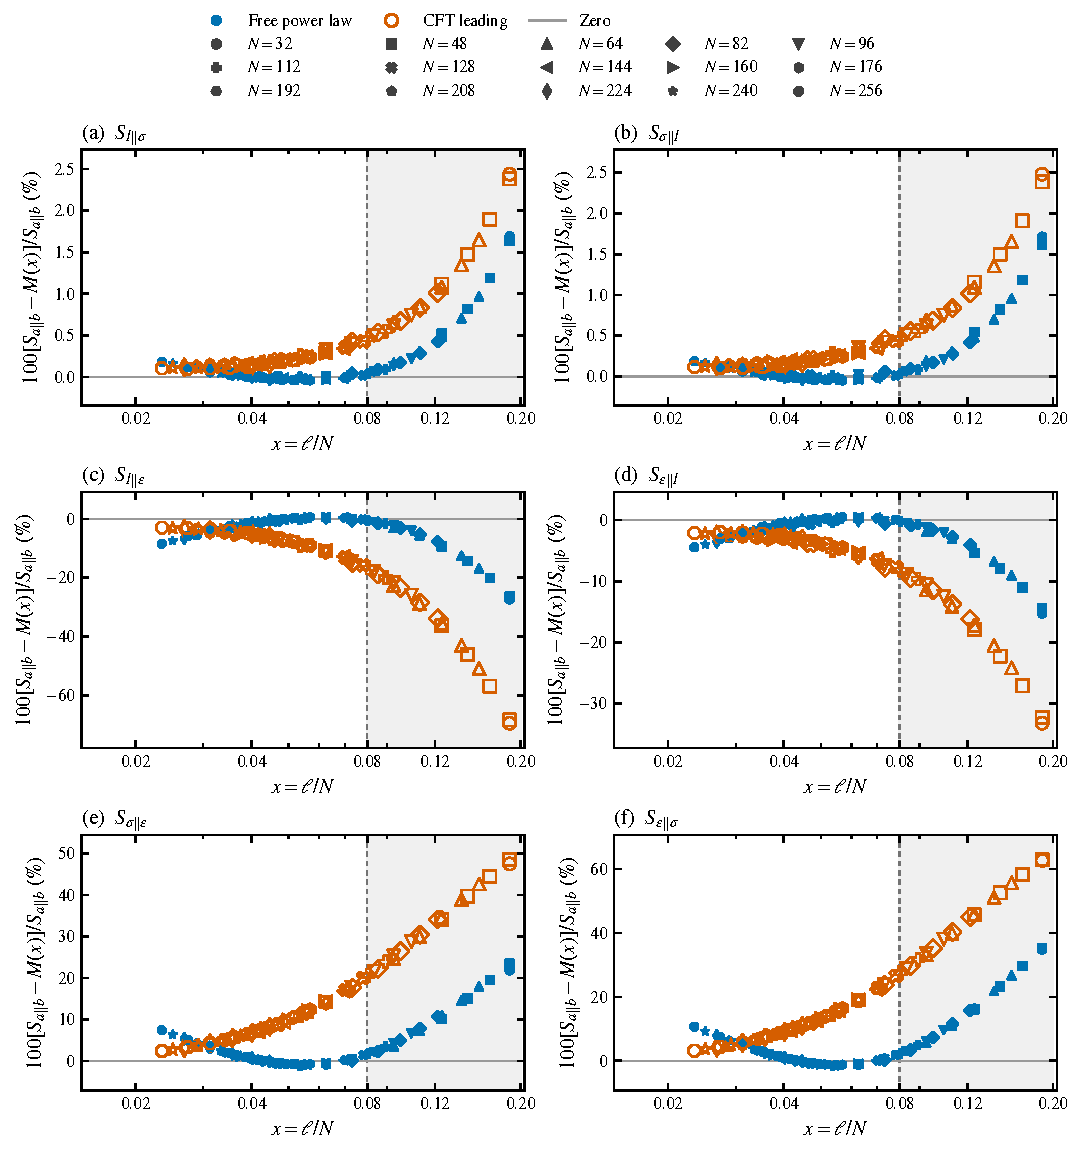
\includegraphics[width=.95\linewidth]{../figs/ising_primary_residuals.pdf}
\caption{Signed percentage residuals for the Ising primary
comparisons in Fig.~\ref{fig:ising-primary-fits}. Blue filled markers
denote the free power law and orange open markers the analytical
leading prediction. Marker shapes identify the 15 sizes in
Eq.~\eqref{eq:large-grid}, with
$\ell=6,\ldots,10$. The ordinate is
$\eta_i=100[S_{a\Vert b}(x_i)-M(x_i)]/S_{a\Vert b}(x_i)$,
where $M=F$ or $F_{\rm CFT}$,
from Eq.~\eqref{eq:primary-fit-residual}; zero means exact agreement.
The ordinate is linear throughout, with ticks showing signed percentage
values directly; $x$ is logarithmic.
All 70 displayed observations per direction satisfy $x\leq0.20$.
Only 51 at $x\leq0.08$ determine the fits and table metrics;
the 19 shaded-region observations test extrapolation.
The free fit has two jointly optimized parameters,
$F=\widehat Cx^{\widehat\alpha}$.
Only the analytical comparison uses $\alpha_{\rm CFT}=4$,
$B_{ab}=8\pi^4/15$ in (c,d), and $\alpha_{\rm CFT}=2$, $B_{ab}=\pi^2/12$
otherwise. The exact PBC Ising states, natural
logarithms and target floor $10^{-15}$ are as in
Fig.~\ref{fig:ising-primary-fits}; coefficients, exponents, RMSE and
CV RMSE appear in Table~\ref{tab:ising-primary-all-fits}.}
\label{fig:ising-primary-residuals}
\end{figure}

\begin{figure}[p]\centering
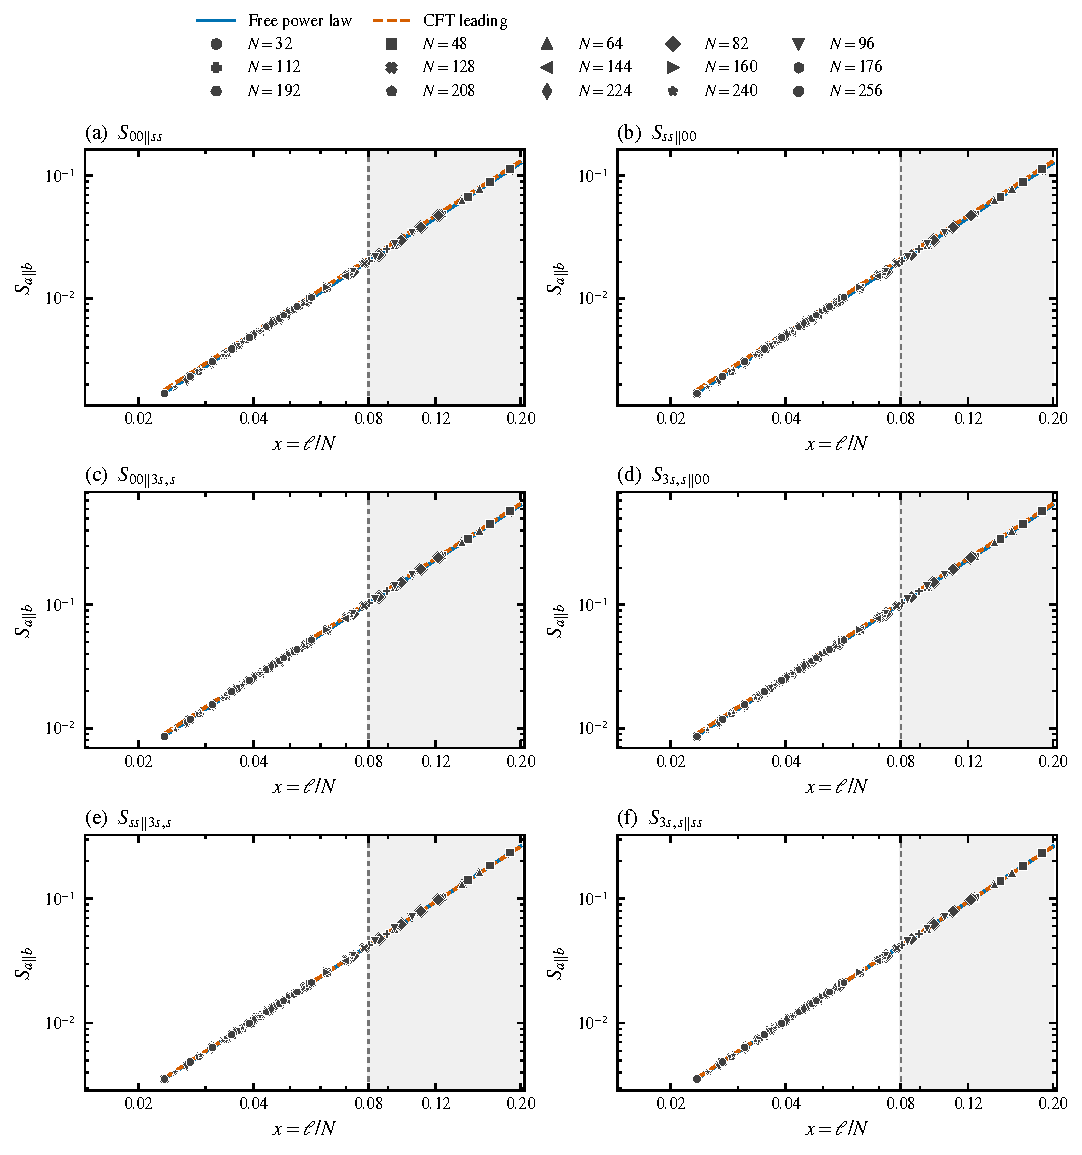
\includegraphics[width=.95\linewidth]{../figs/boson_primary_fits.pdf}
\caption{Historical compact-boson primary relative entropy for all six
directions among charges $(0,0)$, $(s,s)$ and $(3s,s)$,
$s=1/\sqrt2$. Markers identify the 15 sizes through $N=256$
in Eq.~\eqref{eq:large-grid}; $\ell=6,\ldots,10$.
Each panel displays 70 observations at $x\leq0.20$.
The 51 observations at $x\leq0.08$ determine the unweighted
least-squares fits; the vertical line and shading mark the 19
observations outside the fit window. Blue solid lines show
$F=\widehat Cx^{\widehat\alpha}$ from
Eq.~\eqref{eq:primary-fit-ansatz}, with both coefficient and exponent
optimized. Orange dashed lines show the analytical CFT leading-order
predictions, with no fitted parameters: $\alpha_{\rm CFT}=2$ and
$B_{ab}=\pi^2/3$ in (a,b), $5\pi^2/3$ in (c,d), and $2\pi^2/3$ in (e,f).
Table~\ref{tab:boson-primary-all-fits} compares both fitted
parameters with the analytical values.
The normalized vertex/Jastrow states use the unit circle,
$q=2$, $w_1=0$, $W=10^8$, and 100-decimal-digit Pfaffian
construction, without orthogonalization, as in
Sec.~\ref{sec:primary-numerics}.
All logarithms are natural and the target-logarithm floor
is $10^{-15}$. Both axes are logarithmic. The fit has a positive
coefficient and a free real exponent, with no additional terms.}
\label{fig:boson-primary-fits}
\end{figure}

\begin{figure}[p]\centering
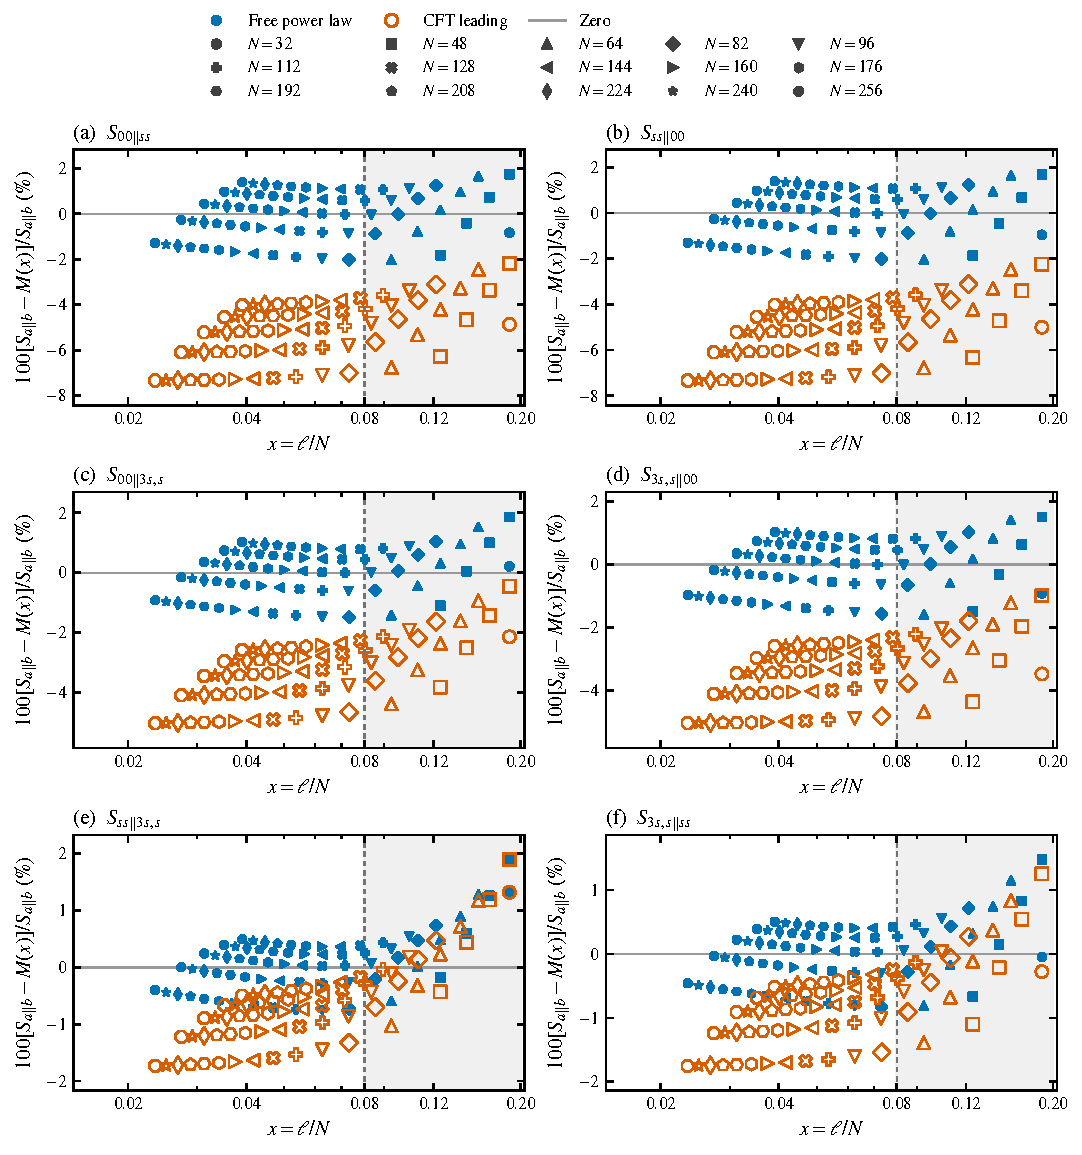
\includegraphics[width=.95\linewidth]{../figs/boson_primary_residuals.pdf}
\caption{Signed percentage residuals for the compact-boson
primary comparisons in Fig.~\ref{fig:boson-primary-fits}.
Blue filled markers denote the free power law; orange open markers
denote the analytical leading term.
The ordinate is $100[S_{a\Vert b}-M]/S_{a\Vert b}$,
where $M=F$ or $F_{\rm CFT}$,
as in Eq.~\eqref{eq:primary-fit-residual}. The vertical scale is linear
throughout, with ticks showing signed percentage values directly;
$x$ is logarithmic. Markers identify the 15 sizes in
Eq.~\eqref{eq:large-grid}, with $\ell=6,\ldots,10$.
All 70 observations per direction at $x\leq0.20$ are shown;
51 at $x\leq0.08$ enter the fits and metrics, while 19 lie
in the shaded extrapolation region. The two-parameter fit is
$F=\widehat Cx^{\widehat\alpha}$; its exponent is not
fixed. The analytical comparison uses $\alpha_{\rm CFT}=2$
and $B_{ab}=\pi^2/3$, $5\pi^2/3$, $2\pi^2/3$ in the top, middle and bottom rows.
The vertex charges, $q=2$,
unit-circle sites, $w_1=0$, $W=10^8$, 100-digit construction,
absence of orthogonalization, natural logarithms and
target floor $10^{-15}$ are as in Fig.~\ref{fig:boson-primary-fits}.
Table~\ref{tab:boson-primary-all-fits} compares fitted coefficients
and exponents with theory and gives RMSE and size-based CV RMSE.}
\label{fig:boson-primary-residuals}
\end{figure}
\clearpage


\clearpage
\section{Parameters and numerical errors for the visual comparisons}
\label{sec:window-appendix}
These tables supplement Sec.~\ref{sec:window-selection}. Models are
grouped by ordered pair, and every fitted row gives its actual interval.
They correspond to both columns of the per-pair figures and the
principal tables in Appendices~\ref{sec:allfits} and
\ref{sec:complement-checks}. The same CFT-wide windows are used throughout.
The coefficient convention and indices follow
Eq.~\eqref{eq:window-models}. Unknown analytical next coefficients
are left blank throughout. Agreement is assessed through the displayed
numerical parameters and curves, without interval-selection labels.

\subsection{Small intervals: Ising}
\begingroup\setlength{\tabcolsep}{2pt}
\begin{longtable}{lllrrrrrrr}
\caption{Ising small intervals: leading parameters for all three models, grouped by ordered pair. Amplitudes multiply $x^r$ itself, including powers of $\pi$. $W_x$ and $m$ give the fitting interval and count. Fixed models impose $r^{(1)}=\alpha_{\rm CFT}$; Free 1 estimates the leading power. Percentage discrepancies use Eq.~\eqref{eq:window-discrepancies}.}
\label{tab:window-small_ising-leading}\\\toprule
Direction & Model & $W_x$ & $m$ & $r^{(1)}_{\rm CFT}$ & $r^{(1)}$ & $c_1^{\rm CFT}$ & $c_1$ & $\eta_{r,1}$ & $\eta_{c,1}$\\\midrule
\endfirsthead
\toprule
Direction & Model & $W_x$ & $m$ & $r^{(1)}_{\rm CFT}$ & $r^{(1)}$ & $c_1^{\rm CFT}$ & $c_1$ & $\eta_{r,1}$ & $\eta_{c,1}$\\\midrule
\endhead
\bottomrule\endfoot
$I\mid \sigma$ & Free 1 & $(0,0.02]$ & 1255 & 2 & 2.0001 & 0.20562 & 0.20585 & 0.0070964 & 0.1146\\*
$I\mid \sigma$ & $F_1$ & $(0,0.02]$ & 1255 & 2 & 2 & 0.20562 & 0.20573 & --- & 0.055265\\*
$I\mid \sigma$ & $F_2$ & $(0,0.02]$ & 1255 & 2 & 2 & 0.20562 & 0.20571 & --- & 0.044771\\
\midrule
$\sigma\mid I$ & Free 1 & $(0,0.02]$ & 1255 & 2 & 2.0001 & 0.20562 & 0.20582 & 0.0057066 & 0.099239\\*
$\sigma\mid I$ & $F_1$ & $(0,0.02]$ & 1255 & 2 & 2 & 0.20562 & 0.20572 & --- & 0.051526\\*
$\sigma\mid I$ & $F_2$ & $(0,0.02]$ & 1255 & 2 & 2 & 0.20562 & 0.2057 & --- & 0.042877\\
\midrule
$I\mid \varepsilon$ & Free 1 & $(0,0.02]$ & 1255 & 4 & 3.9934 & 12.988 & 12.491 & -0.16507 & -3.8239\\*
$I\mid \varepsilon$ & $F_1$ & $(0,0.02]$ & 1255 & 4 & 4 & 12.988 & 12.83 & --- & -1.219\\*
$I\mid \varepsilon$ & $F_2$ & $(0,0.02]$ & 1255 & 4 & 4 & 12.988 & 12.883 & --- & -0.80492\\
\midrule
$\varepsilon\mid I$ & Free 1 & $(0,0.02]$ & 1255 & 4 & 3.9861 & 12.988 & 12.07 & -0.34832 & -7.0661\\*
$\varepsilon\mid I$ & $F_1$ & $(0,0.02]$ & 1255 & 4 & 4 & 12.988 & 12.77 & --- & -1.6748\\*
$\varepsilon\mid I$ & $F_2$ & $(0,0.02]$ & 1255 & 4 & 4 & 12.988 & 12.882 & --- & -0.81263\\
\midrule
$\sigma\mid \varepsilon$ & Free 1 & $(0,0.02]$ & 1255 & 2 & 2.0238 & 0.20562 & 0.23069 & 1.1878 & 12.192\\*
$\sigma\mid \varepsilon$ & $F_1$ & $(0,0.02]$ & 1255 & 2 & 2 & 0.20562 & 0.2089 & --- & 1.595\\*
$\sigma\mid \varepsilon$ & $F_2$ & $(0,0.02]$ & 1255 & 2 & 2 & 0.20562 & 0.20565 & --- & 0.017273\\
\midrule
$\varepsilon\mid \sigma$ & Free 1 & $(0,0.02]$ & 1255 & 2 & 2.0176 & 0.20562 & 0.22393 & 0.88006 & 8.9077\\*
$\varepsilon\mid \sigma$ & $F_1$ & $(0,0.02]$ & 1255 & 2 & 2 & 0.20562 & 0.20806 & --- & 1.1882\\*
$\varepsilon\mid \sigma$ & $F_2$ & $(0,0.02]$ & 1255 & 2 & 2 & 0.20562 & 0.20566 & --- & 0.022414\\
\end{longtable}
\endgroup

\begingroup\setlength{\tabcolsep}{2pt}
\begin{longtable}{lllrrrrrr}
\caption{Ising small intervals: next-order parameters, with $c_2$ multiplying $x^{r^{(2)}}$. $F_2$ imposes both manuscript powers and estimates both coefficients. Empty analytical cells mean that the manuscript does not supply the coefficient. The displayed windows and numerical values also appear in the per-pair figures in Sec.~\ref{sec:pair-small_ising}. Percentage discrepancies use Eq.~\eqref{eq:window-discrepancies}.}
\label{tab:window-small_ising-second}\\\toprule
Direction & Model & $W_x$ & $r^{(2)}_{\rm CFT}$ & $r^{(2)}$ & $c_2^{\rm CFT}$ & $c_2$ & $\eta_{r,2}$ & $\eta_{c,2}$\\\midrule
\endfirsthead
\toprule
Direction & Model & $W_x$ & $r^{(2)}_{\rm CFT}$ & $r^{(2)}$ & $c_2^{\rm CFT}$ & $c_2$ & $\eta_{r,2}$ & $\eta_{c,2}$\\\midrule
\endhead
\bottomrule\endfoot
$I\mid \sigma$ & $F_2$ & $(0,0.02]$ & 4 & 4 &  & 0.083833 & --- & \\*
$\sigma\mid I$ & $F_2$ & $(0,0.02]$ & 4 & 4 &  & 0.069099 & --- & \\*
$I\mid \varepsilon$ & $F_2$ & $(0,0.02]$ & 6 & 6 & -170.91 & -170.71 & --- & -0.12193\\*
$\varepsilon\mid I$ & $F_2$ & $(0,0.02]$ & 6 & 6 & -366.24 & -355.38 & --- & -2.9657\\*
$\sigma\mid \varepsilon$ & $F_2$ & $(0,0.02]$ & 4 & 4 &  & 12.604 & --- & \\*
$\varepsilon\mid \sigma$ & $F_2$ & $(0,0.02]$ & 4 & 4 &  & 9.3133 & --- & \\
\end{longtable}
\endgroup

\begingroup\setlength{\tabcolsep}{2pt}
\begin{longtable}{lllrrrr}
\caption{Ising small intervals: numerical fit errors on each row\textquotesingle s own window. RMSE uses Eq.~\eqref{eq:metrics}; the normalized percentages $E_{\rm fit}$ and $E_{\rm CV}$ use Eq.~\eqref{eq:pair-errors}. The residual plots show pointwise percentages instead. All models and all six directions use the same window for this CFT and interval type.}
\label{tab:window-small_ising-quality}\\\toprule
Direction & Model & $W_x$ & $m$ & RMSE & $E_{\rm fit}$ [\%] & $E_{\rm CV}$ [\%]\\\midrule
\endfirsthead
\toprule
Direction & Model & $W_x$ & $m$ & RMSE & $E_{\rm fit}$ [\%] & $E_{\rm CV}$ [\%]\\\midrule
\endhead
\bottomrule\endfoot
$I\mid \sigma$ & Free 1 & $(0,0.02]$ & 1255 & $5.158\!\times\!10^{-9}$ & 0.017406 & 0.017515\\*
$I\mid \sigma$ & $F_1$ & $(0,0.02]$ & 1255 & $5.249\!\times\!10^{-9}$ & 0.017715 & 0.017787\\*
$I\mid \sigma$ & $F_2$ & $(0,0.02]$ & 1255 & $5.124\!\times\!10^{-9}$ & 0.017292 & 0.017418\\
\midrule
$\sigma\mid I$ & Free 1 & $(0,0.02]$ & 1255 & $4.526\!\times\!10^{-9}$ & 0.015275 & 0.015369\\*
$\sigma\mid I$ & $F_1$ & $(0,0.02]$ & 1255 & $4.594\!\times\!10^{-9}$ & 0.015504 & 0.015565\\*
$\sigma\mid I$ & $F_2$ & $(0,0.02]$ & 1255 & $4.497\!\times\!10^{-9}$ & 0.015175 & 0.015282\\
\midrule
$I\mid \varepsilon$ & Free 1 & $(0,0.02]$ & 1255 & $1.566\!\times\!10^{-9}$ & 0.30918 & 0.31285\\*
$I\mid \varepsilon$ & $F_1$ & $(0,0.02]$ & 1255 & $1.631\!\times\!10^{-9}$ & 0.32198 & 0.32466\\*
$I\mid \varepsilon$ & $F_2$ & $(0,0.02]$ & 1255 & $1.561\!\times\!10^{-9}$ & 0.30816 & 0.31219\\
\midrule
$\varepsilon\mid I$ & Free 1 & $(0,0.02]$ & 1255 & $1.565\!\times\!10^{-9}$ & 0.31025 & 0.3139\\*
$\varepsilon\mid I$ & $F_1$ & $(0,0.02]$ & 1255 & $1.834\!\times\!10^{-9}$ & 0.36374 & 0.36666\\*
$\varepsilon\mid I$ & $F_2$ & $(0,0.02]$ & 1255 & $1.548\!\times\!10^{-9}$ & 0.30693 & 0.31094\\
\midrule
$\sigma\mid \varepsilon$ & Free 1 & $(0,0.02]$ & 1255 & $4.655\!\times\!10^{-8}$ & 0.1547 & 0.15537\\*
$\sigma\mid \varepsilon$ & $F_1$ & $(0,0.02]$ & 1255 & $1.717\!\times\!10^{-7}$ & 0.57076 & 0.57252\\*
$\sigma\mid \varepsilon$ & $F_2$ & $(0,0.02]$ & 1255 & $7.741\!\times\!10^{-9}$ & 0.025729 & 0.025989\\
\midrule
$\varepsilon\mid \sigma$ & Free 1 & $(0,0.02]$ & 1255 & $3.468\!\times\!10^{-8}$ & 0.11573 & 0.11623\\*
$\varepsilon\mid \sigma$ & $F_1$ & $(0,0.02]$ & 1255 & $1.270\!\times\!10^{-7}$ & 0.42368 & 0.42497\\*
$\varepsilon\mid \sigma$ & $F_2$ & $(0,0.02]$ & 1255 & $7.163\!\times\!10^{-9}$ & 0.023901 & 0.024146\\
\end{longtable}
\endgroup

\clearpage
\subsection{Small intervals: compact boson}
\begingroup\setlength{\tabcolsep}{2pt}
\begin{longtable}{lllrrrrrrr}
\caption{Compact boson small intervals: leading parameters for all three models, grouped by ordered pair. Amplitudes multiply $x^r$ itself, including powers of $\pi$. $W_x$ and $m$ give the fitting interval and count. Fixed models impose $r^{(1)}=\alpha_{\rm CFT}$; Free 1 estimates the leading power. Percentage discrepancies use Eq.~\eqref{eq:window-discrepancies}.}
\label{tab:window-small_boson-leading}\\\toprule
Direction & Model & $W_x$ & $m$ & $r^{(1)}_{\rm CFT}$ & $r^{(1)}$ & $c_1^{\rm CFT}$ & $c_1$ & $\eta_{r,1}$ & $\eta_{c,1}$\\\midrule
\endfirsthead
\toprule
Direction & Model & $W_x$ & $m$ & $r^{(1)}_{\rm CFT}$ & $r^{(1)}$ & $c_1^{\rm CFT}$ & $c_1$ & $\eta_{r,1}$ & $\eta_{c,1}$\\\midrule
\endhead
\bottomrule\endfoot
$00\mid ss$ & Free 1 & $(0,0.1]$ & 598 & 2 & 1.9982 & 0.82247 & 0.77501 & -0.092048 & -5.7697\\*
$00\mid ss$ & $F_1$ & $(0,0.1]$ & 598 & 2 & 2 & 0.82247 & 0.77866 & --- & -5.3266\\*
$00\mid ss$ & $F_2$ & $(0,0.1]$ & 598 & 2 & 2 & 0.82247 & 0.77996 & --- & -5.1687\\
\midrule
$ss\mid 00$ & Free 1 & $(0,0.1]$ & 598 & 2 & 1.9983 & 0.82247 & 0.77529 & -0.086511 & -5.7362\\*
$ss\mid 00$ & $F_1$ & $(0,0.1]$ & 598 & 2 & 2 & 0.82247 & 0.77871 & --- & -5.3197\\*
$ss\mid 00$ & $F_2$ & $(0,0.1]$ & 598 & 2 & 2 & 0.82247 & 0.77995 & --- & -5.1696\\
\midrule
$00\mid 3s,s$ & Free 1 & $(0,0.1]$ & 598 & 2 & 1.9649 & 4.1123 & 3.5315 & -1.7561 & -14.124\\*
$00\mid 3s,s$ & $F_1$ & $(0,0.1]$ & 598 & 2 & 2 & 4.1123 & 3.8623 & --- & -6.0813\\*
$00\mid 3s,s$ & $F_2$ & $(0,0.1]$ & 598 & 2 & 2 & 4.1123 & 3.964 & --- & -3.6065\\
\midrule
$3s,s\mid 00$ & Free 1 & $(0,0.1]$ & 598 & 2 & 1.966 & 4.1123 & 3.545 & -1.6988 & -13.795\\*
$3s,s\mid 00$ & $F_1$ & $(0,0.1]$ & 598 & 2 & 2 & 4.1123 & 3.8657 & --- & -5.9968\\*
$3s,s\mid 00$ & $F_2$ & $(0,0.1]$ & 598 & 2 & 2 & 4.1123 & 3.9643 & --- & -3.6009\\
\midrule
$ss\mid 3s,s$ & Free 1 & $(0,0.1]$ & 598 & 2 & 1.9883 & 1.6449 & 1.5661 & -0.58466 & -4.7937\\*
$ss\mid 3s,s$ & $F_1$ & $(0,0.1]$ & 598 & 2 & 2 & 1.6449 & 1.6134 & --- & -1.9141\\*
$ss\mid 3s,s$ & $F_2$ & $(0,0.1]$ & 598 & 2 & 2 & 1.6449 & 1.6276 & --- & -1.0534\\
\midrule
$3s,s\mid ss$ & Free 1 & $(0,0.1]$ & 598 & 2 & 1.9902 & 1.6449 & 1.576 & -0.48899 & -4.1922\\*
$3s,s\mid ss$ & $F_1$ & $(0,0.1]$ & 598 & 2 & 2 & 1.6449 & 1.6157 & --- & -1.7746\\*
$3s,s\mid ss$ & $F_2$ & $(0,0.1]$ & 598 & 2 & 2 & 1.6449 & 1.6276 & --- & -1.0534\\
\end{longtable}
\endgroup

\begingroup\setlength{\tabcolsep}{2pt}
\begin{longtable}{lllrrrrrr}
\caption{Compact boson small intervals: next-order parameters, with $c_2$ multiplying $x^{r^{(2)}}$. $F_2$ imposes both manuscript powers and estimates both coefficients. Empty analytical cells mean that the manuscript does not supply the coefficient. The displayed windows and numerical values also appear in the per-pair figures in Sec.~\ref{sec:pair-small_boson}. Percentage discrepancies use Eq.~\eqref{eq:window-discrepancies}.}
\label{tab:window-small_boson-second}\\\toprule
Direction & Model & $W_x$ & $r^{(2)}_{\rm CFT}$ & $r^{(2)}$ & $c_2^{\rm CFT}$ & $c_2$ & $\eta_{r,2}$ & $\eta_{c,2}$\\\midrule
\endfirsthead
\toprule
Direction & Model & $W_x$ & $r^{(2)}_{\rm CFT}$ & $r^{(2)}$ & $c_2^{\rm CFT}$ & $c_2$ & $\eta_{r,2}$ & $\eta_{c,2}$\\\midrule
\endhead
\bottomrule\endfoot
$00\mid ss$ & $F_2$ & $(0,0.1]$ & 4 & 4 &  & -0.1917 & --- & \\*
$ss\mid 00$ & $F_2$ & $(0,0.1]$ & 4 & 4 &  & -0.18219 & --- & \\*
$00\mid 3s,s$ & $F_2$ & $(0,0.1]$ & 4 & 4 &  & -15.02 & --- & \\*
$3s,s\mid 00$ & $F_2$ & $(0,0.1]$ & 4 & 4 &  & -14.541 & --- & \\*
$ss\mid 3s,s$ & $F_2$ & $(0,0.1]$ & 4 & 4 &  & -2.0896 & --- & \\*
$3s,s\mid ss$ & $F_2$ & $(0,0.1]$ & 4 & 4 &  & -1.7507 & --- & \\
\end{longtable}
\endgroup

\begingroup\setlength{\tabcolsep}{2pt}
\begin{longtable}{lllrrrr}
\caption{Compact boson small intervals: numerical fit errors on each row\textquotesingle s own window. RMSE uses Eq.~\eqref{eq:metrics}; the normalized percentages $E_{\rm fit}$ and $E_{\rm CV}$ use Eq.~\eqref{eq:pair-errors}. The residual plots show pointwise percentages instead. All models and all six directions use the same window for this CFT and interval type.}
\label{tab:window-small_boson-quality}\\\toprule
Direction & Model & $W_x$ & $m$ & RMSE & $E_{\rm fit}$ [\%] & $E_{\rm CV}$ [\%]\\\midrule
\endfirsthead
\toprule
Direction & Model & $W_x$ & $m$ & RMSE & $E_{\rm fit}$ [\%] & $E_{\rm CV}$ [\%]\\\midrule
\endhead
\bottomrule\endfoot
$00\mid ss$ & Free 1 & $(0,0.1]$ & 598 & $1.742\!\times\!10^{-5}$ & 1.0869 & 1.1352\\*
$00\mid ss$ & $F_1$ & $(0,0.1]$ & 598 & $1.744\!\times\!10^{-5}$ & 1.0879 & 1.1167\\*
$00\mid ss$ & $F_2$ & $(0,0.1]$ & 598 & $1.741\!\times\!10^{-5}$ & 1.0862 & 1.1453\\
\midrule
$ss\mid 00$ & Free 1 & $(0,0.1]$ & 598 & $1.737\!\times\!10^{-5}$ & 1.0838 & 1.1319\\*
$ss\mid 00$ & $F_1$ & $(0,0.1]$ & 598 & $1.739\!\times\!10^{-5}$ & 1.0847 & 1.1133\\*
$ss\mid 00$ & $F_2$ & $(0,0.1]$ & 598 & $1.736\!\times\!10^{-5}$ & 1.0832 & 1.142\\
\midrule
$00\mid 3s,s$ & Free 1 & $(0,0.1]$ & 598 & $6.866\!\times\!10^{-5}$ & 0.86378 & 0.90223\\*
$00\mid 3s,s$ & $F_1$ & $(0,0.1]$ & 598 & $9.993\!\times\!10^{-5}$ & 1.2571 & 1.2969\\*
$00\mid 3s,s$ & $F_2$ & $(0,0.1]$ & 598 & $6.343\!\times\!10^{-5}$ & 0.79788 & 0.84032\\
\midrule
$3s,s\mid 00$ & Free 1 & $(0,0.1]$ & 598 & $6.562\!\times\!10^{-5}$ & 0.82472 & 0.86069\\*
$3s,s\mid 00$ & $F_1$ & $(0,0.1]$ & 598 & $9.614\!\times\!10^{-5}$ & 1.2083 & 1.2463\\*
$3s,s\mid 00$ & $F_2$ & $(0,0.1]$ & 598 & $6.045\!\times\!10^{-5}$ & 0.75982 & 0.7993\\
\midrule
$ss\mid 3s,s$ & Free 1 & $(0,0.1]$ & 598 & $1.453\!\times\!10^{-5}$ & 0.43746 & 0.45738\\*
$ss\mid 3s,s$ & $F_1$ & $(0,0.1]$ & 598 & $1.765\!\times\!10^{-5}$ & 0.53149 & 0.54888\\*
$ss\mid 3s,s$ & $F_2$ & $(0,0.1]$ & 598 & $1.400\!\times\!10^{-5}$ & 0.42169 & 0.4446\\
\midrule
$3s,s\mid ss$ & Free 1 & $(0,0.1]$ & 598 & $1.241\!\times\!10^{-5}$ & 0.37329 & 0.38904\\*
$3s,s\mid ss$ & $F_1$ & $(0,0.1]$ & 598 & $1.498\!\times\!10^{-5}$ & 0.45055 & 0.46479\\*
$3s,s\mid ss$ & $F_2$ & $(0,0.1]$ & 598 & $1.198\!\times\!10^{-5}$ & 0.3602 & 0.3782\\
\end{longtable}
\endgroup

\clearpage
\subsection{Large intervals: Ising}
\begingroup\setlength{\tabcolsep}{2pt}
\begin{longtable}{lllrrrrrrr}
\caption{Ising large intervals: leading parameters for all three models, grouped by ordered pair. Amplitudes multiply $y^r$ itself, including powers of $\pi$. $W_y$ and $m$ give the fitting interval and count. Fixed models impose $r^{(1)}=\beta_{\rm CFT}$; Free 1 estimates the leading power. Percentage discrepancies use Eq.~\eqref{eq:window-discrepancies}.}
\label{tab:window-large_ising-leading}\\\toprule
Direction & Model & $W_y$ & $m$ & $r^{(1)}_{\rm CFT}$ & $r^{(1)}$ & $c_1^{\rm CFT}$ & $c_1$ & $\eta_{r,1}$ & $\eta_{c,1}$\\\midrule
\endfirsthead
\toprule
Direction & Model & $W_y$ & $m$ & $r^{(1)}_{\rm CFT}$ & $r^{(1)}$ & $c_1^{\rm CFT}$ & $c_1$ & $\eta_{r,1}$ & $\eta_{c,1}$\\\midrule
\endhead
\bottomrule\endfoot
$I\mid \sigma$ & Free 1 & $(0,0.002]$ & 260 & 0.25 & 0.26465 & 0.61965 & 0.71994 & 5.8606 & 16.184\\*
$I\mid \sigma$ & $F_1$ & $(0,0.002]$ & 260 & 0.25 & 0.25 & 0.61965 & 0.65339 & --- & 5.4442\\*
$I\mid \sigma$ & $F_2$ & $(0,0.002]$ & 260 & 0.25 & 0.25 & 0.61965 & 0.61463 & --- & -0.81098\\
\midrule
$\sigma\mid I$ & Free 1 & $(0,0.002]$ & 260 & 0.25 & 0.26465 & 0.61965 & 0.71995 & 5.8612 & 16.186\\*
$\sigma\mid I$ & $F_1$ & $(0,0.002]$ & 260 & 0.25 & 0.25 & 0.61965 & 0.65339 & --- & 5.4445\\*
$\sigma\mid I$ & $F_2$ & $(0,0.002]$ & 260 & 0.25 & 0.25 & 0.61965 & 0.61462 & --- & -0.81139\\
\midrule
$I\mid \varepsilon$ & Free 1 & $(0,0.002]$ & 260 & 2 & 1.9985 & 3.2899 & 3.2548 & -0.074487 & -1.0674\\*
$I\mid \varepsilon$ & $F_1$ & $(0,0.002]$ & 260 & 2 & 2 & 3.2899 & 3.2861 & --- & -0.11533\\*
$I\mid \varepsilon$ & $F_2$ & $(0,0.002]$ & 260 & 2 & 2 & 3.2899 & 3.289 & --- & -0.024918\\
\midrule
$\varepsilon\mid I$ & Free 1 & $(0,0.002]$ & 260 & 2 & 2.0013 & 3.2899 & 3.3242 & 0.065315 & 1.0443\\*
$\varepsilon\mid I$ & $F_1$ & $(0,0.002]$ & 260 & 2 & 2 & 3.2899 & 3.2964 & --- & 0.19921\\*
$\varepsilon\mid I$ & $F_2$ & $(0,0.002]$ & 260 & 2 & 2 & 3.2899 & 3.2938 & --- & 0.11818\\
\midrule
$\sigma\mid \varepsilon$ & Free 1 & $(0,0.002]$ & 260 & 0.25 & 0.25058 & 0.15491 & 0.15691 & 0.23227 & 1.2904\\*
$\sigma\mid \varepsilon$ & $F_1$ & $(0,0.002]$ & 260 & 0.25 & 0.25 & 0.15491 & 0.15631 & --- & 0.9017\\*
$\sigma\mid \varepsilon$ & $F_2$ & $(0,0.002]$ & 260 & 0.25 & 0.25 & 0.15491 & 0.15595 & --- & 0.67037\\
\midrule
$\varepsilon\mid \sigma$ & Free 1 & $(0,0.002]$ & 260 & 0.25 & 0.25544 & 0.15491 & 0.16288 & 2.1754 & 5.1411\\*
$\varepsilon\mid \sigma$ & $F_1$ & $(0,0.002]$ & 260 & 0.25 & 0.25 & 0.15491 & 0.15712 & --- & 1.4228\\*
$\varepsilon\mid \sigma$ & $F_2$ & $(0,0.002]$ & 260 & 0.25 & 0.25 & 0.15491 & 0.15365 & --- & -0.81285\\
\end{longtable}
\endgroup

\begingroup\setlength{\tabcolsep}{2pt}
\begin{longtable}{lllrrrrrr}
\caption{Ising large intervals: next-order parameters, with $c_2$ multiplying $y^{r^{(2)}}$. $F_2$ imposes both manuscript powers and estimates both coefficients. Empty analytical cells mean that the manuscript does not supply the coefficient. The displayed windows and numerical values also appear in the per-pair figures in Sec.~\ref{sec:pair-large_ising}. Percentage discrepancies use Eq.~\eqref{eq:window-discrepancies}.}
\label{tab:window-large_ising-second}\\\toprule
Direction & Model & $W_y$ & $r^{(2)}_{\rm CFT}$ & $r^{(2)}$ & $c_2^{\rm CFT}$ & $c_2$ & $\eta_{r,2}$ & $\eta_{c,2}$\\\midrule
\endfirsthead
\toprule
Direction & Model & $W_y$ & $r^{(2)}_{\rm CFT}$ & $r^{(2)}$ & $c_2^{\rm CFT}$ & $c_2$ & $\eta_{r,2}$ & $\eta_{c,2}$\\\midrule
\endhead
\bottomrule\endfoot
$I\mid \sigma$ & $F_2$ & $(0,0.002]$ & 0.5 & 0.5 &  & 0.20243 & --- & \\*
$\sigma\mid I$ & $F_2$ & $(0,0.002]$ & 0.5 & 0.5 &  & 0.20245 & --- & \\*
$I\mid \varepsilon$ & $F_2$ & $(0,0.002]$ & 4 & 4 &  & -1070.2 & --- & \\*
$\varepsilon\mid I$ & $F_2$ & $(0,0.002]$ & 4 & 4 &  & 959.21 & --- & \\*
$\sigma\mid \varepsilon$ & $F_2$ & $(0,0.002]$ & 0.5 & 0.5 &  & 0.0018716 & --- & \\*
$\varepsilon\mid \sigma$ & $F_2$ & $(0,0.002]$ & 0.5 & 0.5 &  & 0.018087 & --- & \\
\end{longtable}
\endgroup

\begingroup\setlength{\tabcolsep}{2pt}
\begin{longtable}{lllrrrr}
\caption{Ising large intervals: numerical fit errors on each row\textquotesingle s own window. RMSE uses Eq.~\eqref{eq:metrics}; the normalized percentages $E_{\rm fit}$ and $E_{\rm CV}$ use Eq.~\eqref{eq:pair-errors}. The residual plots show pointwise percentages instead. All models and all six directions use the same window for this CFT and interval type.}
\label{tab:window-large_ising-quality}\\\toprule
Direction & Model & $W_y$ & $m$ & RMSE & $E_{\rm fit}$ [\%] & $E_{\rm CV}$ [\%]\\\midrule
\endfirsthead
\toprule
Direction & Model & $W_y$ & $m$ & RMSE & $E_{\rm fit}$ [\%] & $E_{\rm CV}$ [\%]\\\midrule
\endhead
\bottomrule\endfoot
$I\mid \sigma$ & Free 1 & $(0,0.002]$ & 260 & $2.156\!\times\!10^{-5}$ & 0.017352 & 0.01755\\*
$I\mid \sigma$ & $F_1$ & $(0,0.002]$ & 260 & $4.858\!\times\!10^{-4}$ & 0.39088 & 0.39445\\*
$I\mid \sigma$ & $F_2$ & $(0,0.002]$ & 260 & $1.523\!\times\!10^{-5}$ & 0.012258 & 0.012375\\
\midrule
$\sigma\mid I$ & Free 1 & $(0,0.002]$ & 260 & $2.150\!\times\!10^{-5}$ & 0.017302 & 0.0175\\*
$\sigma\mid I$ & $F_1$ & $(0,0.002]$ & 260 & $4.858\!\times\!10^{-4}$ & 0.39091 & 0.39449\\*
$\sigma\mid I$ & $F_2$ & $(0,0.002]$ & 260 & $1.512\!\times\!10^{-5}$ & 0.012167 & 0.012282\\
\midrule
$I\mid \varepsilon$ & Free 1 & $(0,0.002]$ & 260 & $1.190\!\times\!10^{-9}$ & 0.017016 & 0.017287\\*
$I\mid \varepsilon$ & $F_1$ & $(0,0.002]$ & 260 & $2.346\!\times\!10^{-9}$ & 0.033562 & 0.033674\\*
$I\mid \varepsilon$ & $F_2$ & $(0,0.002]$ & 260 & $1.217\!\times\!10^{-9}$ & 0.017404 & 0.01769\\
\midrule
$\varepsilon\mid I$ & Free 1 & $(0,0.002]$ & 260 & $9.799\!\times\!10^{-10}$ & 0.013973 & 0.014171\\*
$\varepsilon\mid I$ & $F_1$ & $(0,0.002]$ & 260 & $2.030\!\times\!10^{-9}$ & 0.028953 & 0.029255\\*
$\varepsilon\mid I$ & $F_2$ & $(0,0.002]$ & 260 & $9.430\!\times\!10^{-10}$ & 0.013446 & 0.013677\\
\midrule
$\sigma\mid \varepsilon$ & Free 1 & $(0,0.002]$ & 260 & $5.939\!\times\!10^{-6}$ & 0.019975 & 0.020151\\*
$\sigma\mid \varepsilon$ & $F_1$ & $(0,0.002]$ & 260 & $7.515\!\times\!10^{-6}$ & 0.025277 & 0.025317\\*
$\sigma\mid \varepsilon$ & $F_2$ & $(0,0.002]$ & 260 & $6.027\!\times\!10^{-6}$ & 0.020272 & 0.020447\\
\midrule
$\varepsilon\mid \sigma$ & Free 1 & $(0,0.002]$ & 260 & $4.604\!\times\!10^{-6}$ & 0.015407 & 0.015572\\*
$\varepsilon\mid \sigma$ & $F_1$ & $(0,0.002]$ & 260 & $4.358\!\times\!10^{-5}$ & 0.14583 & 0.14705\\*
$\varepsilon\mid \sigma$ & $F_2$ & $(0,0.002]$ & 260 & $4.134\!\times\!10^{-6}$ & 0.013835 & 0.013973\\
\end{longtable}
\endgroup

\clearpage
\subsection{Large intervals: compact boson}
\begingroup\setlength{\tabcolsep}{2pt}
\begin{longtable}{lllrrrrrrr}
\caption{Compact boson large intervals: leading parameters for all three models, grouped by ordered pair. Amplitudes multiply $y^r$ itself, including powers of $\pi$. $W_y$ and $m$ give the fitting interval and count. Fixed models impose $r^{(1)}=\beta_{\rm CFT}$; Free 1 estimates the leading power. Percentage discrepancies use Eq.~\eqref{eq:window-discrepancies}.}
\label{tab:window-large_boson-leading}\\\toprule
Direction & Model & $W_y$ & $m$ & $r^{(1)}_{\rm CFT}$ & $r^{(1)}$ & $c_1^{\rm CFT}$ & $c_1$ & $\eta_{r,1}$ & $\eta_{c,1}$\\\midrule
\endfirsthead
\toprule
Direction & Model & $W_y$ & $m$ & $r^{(1)}_{\rm CFT}$ & $r^{(1)}$ & $c_1^{\rm CFT}$ & $c_1$ & $\eta_{r,1}$ & $\eta_{c,1}$\\\midrule
\endhead
\bottomrule\endfoot
$00\mid ss$ & Free 1 & $(0,0.005]$ & 317 & 1 & 0.99926 & 1.2337 & 1.2561 & -0.07446 & 1.8189\\*
$00\mid ss$ & $F_1$ & $(0,0.005]$ & 317 & 1 & 1 & 1.2337 & 1.2616 & --- & 2.2645\\*
$00\mid ss$ & $F_2$ & $(0,0.005]$ & 317 & 1 & 1 & 1.2337 & 1.2627 & --- & 2.3499\\
\midrule
$ss\mid 00$ & Free 1 & $(0,0.005]$ & 317 & 1 & 0.99924 & 1.2337 & 1.256 & -0.075663 & 1.8109\\*
$ss\mid 00$ & $F_1$ & $(0,0.005]$ & 317 & 1 & 1 & 1.2337 & 1.2616 & --- & 2.2636\\*
$ss\mid 00$ & $F_2$ & $(0,0.005]$ & 317 & 1 & 1 & 1.2337 & 1.2627 & --- & 2.351\\
\midrule
$00\mid 3s,s$ & Free 1 & $(0,0.005]$ & 317 & 5 & 4.9836 & 75.109 & 66.924 & -0.32701 & -10.897\\*
$00\mid 3s,s$ & $F_1$ & $(0,0.005]$ & 317 & 5 & 5 & 75.109 & 73.093 & --- & -2.6829\\*
$00\mid 3s,s$ & $F_2$ & $(0,0.005]$ & 317 & 5 & 5 & 75.109 & 74.307 & --- & -1.0676\\
\midrule
$3s,s\mid 00$ & Free 1 & $(0,0.005]$ & 317 & 5 & 4.9838 & 75.109 & 66.96 & -0.32323 & -10.849\\*
$3s,s\mid 00$ & $F_1$ & $(0,0.005]$ & 317 & 5 & 5 & 75.109 & 73.058 & --- & -2.7295\\*
$3s,s\mid 00$ & $F_2$ & $(0,0.005]$ & 317 & 5 & 5 & 75.109 & 74.252 & --- & -1.141\\
\midrule
$ss\mid 3s,s$ & Free 1 & $(0,0.005]$ & 317 & 2 & 1.9914 & 3.2899 & 3.069 & -0.42763 & -6.7143\\*
$ss\mid 3s,s$ & $F_1$ & $(0,0.005]$ & 317 & 2 & 2 & 3.2899 & 3.2185 & --- & -2.1683\\*
$ss\mid 3s,s$ & $F_2$ & $(0,0.005]$ & 317 & 2 & 2 & 3.2899 & 3.2529 & --- & -1.1234\\
\midrule
$3s,s\mid ss$ & Free 1 & $(0,0.005]$ & 317 & 2 & 1.9912 & 3.2899 & 3.0643 & -0.43847 & -6.8552\\*
$3s,s\mid ss$ & $F_1$ & $(0,0.005]$ & 317 & 2 & 2 & 3.2899 & 3.2176 & --- & -2.1982\\*
$3s,s\mid ss$ & $F_2$ & $(0,0.005]$ & 317 & 2 & 2 & 3.2899 & 3.2528 & --- & -1.1274\\
\end{longtable}
\endgroup

\begingroup\setlength{\tabcolsep}{2pt}
\begin{longtable}{lllrrrrrr}
\caption{Compact boson large intervals: next-order parameters, with $c_2$ multiplying $y^{r^{(2)}}$. $F_2$ imposes both manuscript powers and estimates both coefficients. Empty analytical cells mean that the manuscript does not supply the coefficient. The displayed windows and numerical values also appear in the per-pair figures in Sec.~\ref{sec:pair-large_boson}. Percentage discrepancies use Eq.~\eqref{eq:window-discrepancies}.}
\label{tab:window-large_boson-second}\\\toprule
Direction & Model & $W_y$ & $r^{(2)}_{\rm CFT}$ & $r^{(2)}$ & $c_2^{\rm CFT}$ & $c_2$ & $\eta_{r,2}$ & $\eta_{c,2}$\\\midrule
\endfirsthead
\toprule
Direction & Model & $W_y$ & $r^{(2)}_{\rm CFT}$ & $r^{(2)}$ & $c_2^{\rm CFT}$ & $c_2$ & $\eta_{r,2}$ & $\eta_{c,2}$\\\midrule
\endhead
\bottomrule\endfoot
$00\mid ss$ & $F_2$ & $(0,0.005]$ & 2 & 2 &  & -0.33376 & --- & \\*
$ss\mid 00$ & $F_2$ & $(0,0.005]$ & 2 & 2 &  & -0.34138 & --- & \\*
$00\mid 3s,s$ & $F_2$ & $(0,0.005]$ & 6 & 6 &  & -265.58 & --- & \\*
$3s,s\mid 00$ & $F_2$ & $(0,0.005]$ & 6 & 6 &  & -261.18 & --- & \\*
$ss\mid 3s,s$ & $F_2$ & $(0,0.005]$ & 3 & 3 &  & -8.6617 & --- & \\*
$3s,s\mid ss$ & $F_2$ & $(0,0.005]$ & 3 & 3 &  & -8.8758 & --- & \\
\end{longtable}
\endgroup

\begingroup\setlength{\tabcolsep}{2pt}
\begin{longtable}{lllrrrr}
\caption{Compact boson large intervals: numerical fit errors on each row\textquotesingle s own window. RMSE uses Eq.~\eqref{eq:metrics}; the normalized percentages $E_{\rm fit}$ and $E_{\rm CV}$ use Eq.~\eqref{eq:pair-errors}. The residual plots show pointwise percentages instead. All models and all six directions use the same window for this CFT and interval type.}
\label{tab:window-large_boson-quality}\\\toprule
Direction & Model & $W_y$ & $m$ & RMSE & $E_{\rm fit}$ [\%] & $E_{\rm CV}$ [\%]\\\midrule
\endfirsthead
\toprule
Direction & Model & $W_y$ & $m$ & RMSE & $E_{\rm fit}$ [\%] & $E_{\rm CV}$ [\%]\\\midrule
\endhead
\bottomrule\endfoot
$00\mid ss$ & Free 1 & $(0,0.005]$ & 317 & $1.023\!\times\!10^{-5}$ & 0.40141 & 0.4069\\*
$00\mid ss$ & $F_1$ & $(0,0.005]$ & 317 & $1.028\!\times\!10^{-5}$ & 0.40315 & 0.40552\\*
$00\mid ss$ & $F_2$ & $(0,0.005]$ & 317 & $1.024\!\times\!10^{-5}$ & 0.40179 & 0.40879\\
\midrule
$ss\mid 00$ & Free 1 & $(0,0.005]$ & 317 & $1.014\!\times\!10^{-5}$ & 0.39781 & 0.40329\\*
$ss\mid 00$ & $F_1$ & $(0,0.005]$ & 317 & $1.019\!\times\!10^{-5}$ & 0.39963 & 0.40199\\*
$ss\mid 00$ & $F_2$ & $(0,0.005]$ & 317 & $1.015\!\times\!10^{-5}$ & 0.39819 & 0.40517\\
\midrule
$00\mid 3s,s$ & Free 1 & $(0,0.005]$ & 317 & $3.500\!\times\!10^{-13}$ & 0.87692 & 0.94986\\*
$00\mid 3s,s$ & $F_1$ & $(0,0.005]$ & 317 & $3.558\!\times\!10^{-13}$ & 0.89163 & 0.94989\\*
$00\mid 3s,s$ & $F_2$ & $(0,0.005]$ & 317 & $3.508\!\times\!10^{-13}$ & 0.87912 & 0.95369\\
\midrule
$3s,s\mid 00$ & Free 1 & $(0,0.005]$ & 317 & $3.580\!\times\!10^{-13}$ & 0.89749 & 0.97157\\*
$3s,s\mid 00$ & $F_1$ & $(0,0.005]$ & 317 & $3.636\!\times\!10^{-13}$ & 0.91154 & 0.97081\\*
$3s,s\mid 00$ & $F_2$ & $(0,0.005]$ & 317 & $3.589\!\times\!10^{-13}$ & 0.8997 & 0.9754\\
\midrule
$ss\mid 3s,s$ & Free 1 & $(0,0.005]$ & 317 & $8.501\!\times\!10^{-8}$ & 0.38482 & 0.39943\\*
$ss\mid 3s,s$ & $F_1$ & $(0,0.005]$ & 317 & $1.005\!\times\!10^{-7}$ & 0.45481 & 0.46774\\*
$ss\mid 3s,s$ & $F_2$ & $(0,0.005]$ & 317 & $8.538\!\times\!10^{-8}$ & 0.3865 & 0.40258\\
\midrule
$3s,s\mid ss$ & Free 1 & $(0,0.005]$ & 317 & $8.761\!\times\!10^{-8}$ & 0.39671 & 0.4119\\*
$3s,s\mid ss$ & $F_1$ & $(0,0.005]$ & 317 & $1.034\!\times\!10^{-7}$ & 0.46815 & 0.48153\\*
$3s,s\mid ss$ & $F_2$ & $(0,0.005]$ & 317 & $8.800\!\times\!10^{-8}$ & 0.39847 & 0.4152\\
\end{longtable}
\endgroup


\clearpage
\subsection{Sanity checks and reproducibility}
\label{sec:window-reproduction}
For each retained window, the two-term residual is checked against
the matching one-term residual, since that model is nested in the
two-term family. Fixed coefficients are independently checked by
column-normalized normal equations.
Original entropy values are checked against the pre-revision snapshot;
the added system sizes extend those raw records. The $\ell=4,5$ values
remain archived and enter neither the fitted nor displayed data.
The principal fitted rows in Appendices~\ref{sec:allfits} and
\ref{sec:complement-checks} adopt the common CFT-wide windows
in Eq.~\eqref{eq:common-fit-windows}. Their coefficients and omitted-size errors are refitted
independently from the entropy CSV; every fit and training fold has at
least forty observations. All three fitted models share an interval
across all six directions of each CFT and interval type. CFT coefficients remain analytical
inputs, while its residual metrics use the common-window data mask.
The dense-scan window choices are recorded explicitly.

The numerical record contains the following files:
\begin{itemize}
\item \path{window_scan.csv}: the historical window-scan record.
\item \path{window_selected.csv}: selected windows, complete parameters,
and observation counts; the report reads only Free 1, $F_1$, and $F_2$.
\item \path{window_retained_cv.csv}: omitted-size refits for the current
companion visualization records (the same common-window fits).
\item \path{retained_window_specifications.json}: current explicit window
endpoints, checked against every current principal and varied fit.
\item \path{selection_raw_preservation.json} and
\path{selection_audit.json}: raw-data preservation and current audits.
\item \path{f2_summary_fits.csv}: revised principal tables, with
CFT-wide windows for all three models and matched-window gains.
\item \path{f2_summary_cv.csv}: all principal models and reference $F_1$
omitted-size refits; \path{f2_summary_comparison.csv} records common-window
and companion $F_2$ coefficients, which now coincide.
\end{itemize}
Conditional least-squares
standard errors in the CSVs are descriptive local-curvature measures,
not statistical confidence intervals for these deterministic data.

The complete numerical implementation is
\texttt{src/conformal\_blocks/retained\_window\_fits.py}; plotting and TeX
generation are in \texttt{report/pair\_fit\_artifacts.py}.
Using the already approved interpreter and threading settings in
\texttt{SCALING\_README.md}, run
\begin{verbatim}
python report/rebuild_report.py
python report/selection_audit.py
\end{verbatim}
Then compile \texttt{main.tex} three times and package with the
existing report audit. The visualization reads the supplied entropy and fit
CSVs directly and does not require the wavefunction caches. The
manuscript is identified by source hash and citation, not redistributed
in the Overleaf archive.

\clearpage
\section{Dense sampling and the second manuscript term}
\label{sec:dense-second-order}
The purpose of this scan is to distinguish an improved residual from
an improved estimate of a CFT coefficient. In particular, adding a
second basis function always reduces the training sum of squares, but
need not move the first coefficient towards its theoretical value.
We therefore compare $F_1$ and $F_2$ on exactly the same observations,
using the objective in Eq.~\eqref{eq:objective}, and examine both
coefficients rather than the residual alone.

\subsection{Additional geometries and direct coefficient comparisons}
Both CFTs first receive the same additional 47 even sizes between 60 and
6000. Start with $N_j=2\operatorname{round}[30\,100^{j/48}]$ for
$j=0,\ldots,48$, and omit sizes already present. Every new size uses
$\ell=6,7,8,9,10$ and computes both interval observables for all six
ordered pairs. A further 188 Ising sizes complete the progression
$N=200,204,\ldots,1000$, concentrating observations where the known
$x^6$ term is measurable. The two sets are defined in
Eq.~\eqref{eq:dense-grid}. No new size exceeds the existing maxima
8192 and 16384. The resulting 1175 Ising and 235 boson new geometries per direction fill
the intermediate fractions without changing any previously computed
entropy. The exact executed sizes, checks, and timings are retained
in \path{data/dense_grid_manifest.json} and the production CSVs.
The subsequent refinement in Appendix~\ref{sec:common-window-results}
adds 48 further sizes for each CFT while keeping all fitting windows
fixed. Every current fit, plotted coefficient and window-sensitivity
comparison below uses the combined data; the two grid manifests
distinguish the original dense scan from this later refinement.

Let $q=D^A$ with $z=x$ for a small interval, or
$q=\delta=\log 2-D^B$ with $z=y$ for its large complement. With the
pair-specific powers $r_0,r_1$ in Eq.~\eqref{eq:fit}, the two models are
$F_1=c_0z^{r_0}$ and $F_2=c_0z^{r_0}+c_1z^{r_1}$.
Both coefficients in $F_2$ are estimated; neither is fixed to theory.
All amplitudes include their powers of $\pi$.
For the leading discrepancy $\eta_c$ in Eq.~\eqref{eq:metrics}, define
\begin{equation}
 \Delta_0=|\eta_c(F_1)|-|\eta_c(F_2)|.
 \label{eq:dense-coefficient-gain}
\end{equation}
A positive $\Delta_0$, measured in percentage points, means that
including the second term improves the leading coefficient on that
window. This is distinct from the residual gain $G$ and the omitted-size
prediction gain $G_{\rm CV}$. All reported fits and omitted-size
training sets retain at least forty observations.

For the known Ising coefficients, the supplied manuscript gives
\begin{align}
 D^A_{I\mid\eps}&=\frac{2\pi^4}{15}x^4-\frac{8\pi^6}{45}x^6+O(x^8),\nonumber\\
 D^A_{\eps\mid I}&=\frac{2\pi^4}{15}x^4-\frac{8\pi^6}{21}x^6+O(x^8).
 \label{eq:dense-known-ising}
\end{align}
These are the $p=1/2$ specializations of the two Ising mixture
expressions in the supplied source~\cite{theoryLarge}. No missing
subleading coefficient is derived or assumed. The unknown analytical
cells remain blank.

\subsection{What is resolved by the dense scan}
The principal comparisons improve the absolute leading-coefficient discrepancy in 22 of the 24 ordered-pair/interval cases. Of these, 18 also improve the omitted-size prediction residual. Tables~\ref{tab:dense-small-ising}--\ref{tab:dense-large-boson-second} retain the failures as well as the improvements. A lower residual alone is therefore not counted as recovery of a CFT coefficient.

For boson large intervals, $00\mid ss$ on $W=(0,0.005]$ changes the leading discrepancy from $2.2645\%$ under $F_1$ to $2.3499\%$ under $F_2$. This is a failure to improve that coefficient, even if the residual decreases.

For boson large intervals, $ss\mid 00$ on $W=(0,0.005]$ changes the leading discrepancy from $2.2636\%$ under $F_1$ to $2.351\%$ under $F_2$. This is a failure to improve that coefficient, even if the residual decreases.

The adopted windows are Eq.~\eqref{eq:common-fit-windows}. The large-boson upper cutoff is prescribed as $0.005$: Appendix~\ref{sec:common-window-results} reports its neighboring-cutoff and omitted-size sensitivity. Improvement of a leading coefficient does not establish recovery of its unknown second coefficient.

For the two known Ising directions, the pooled window $W_x=(0,0.02]$ gives $c_1=-170.71$ and $-355.38$, respectively. Their signed discrepancies from Eq.~\eqref{eq:dense-known-ising} are $-0.12193\%$ and $-2.9657\%$. The leading coefficient improves in 2 of these two directions; the omitted-size ranges in Table~\ref{tab:dense-small-ising-second} expose the remaining sensitivity of the pooled second coefficients.

At $\ell=10$, the separate-length fits on $W_x=(0,0.006]$ contain 82 points each and give $c_1=-169.27$ and $-362.08$. Their discrepancies are $-0.96408\%$ and $-1.1357\%$. The leading coefficients differ from theory by about $0.49974\%$. The dependence on $\ell$ and on the upper endpoint is visible in Fig.~\ref{fig:dense-subsystem}; these small omitted-size ranges do not erase the finite-length offset.

The cutoff propagation in Eq.~\eqref{eq:dense-cutoff-bound} gives $b_1=0.0027612$ and $0.0027345$ for the same $\ell=10$ fits. The recorded cutoff variation is much smaller than the observed second-coefficient discrepancy. These values are sensitivity bounds for the tested cutoff variation only.

The separate shared-window diagnostic uses $W_x=W_y=(0,0.006]$ and improves the leading coefficient in 21 of 24 cases; see Fig.~\ref{fig:dense-shared}. Across all 744 common windows in the recorded scan on the current grid, the largest improvement count is 23 of 24. No single interval in that scan improves all pairs simultaneously. This does not preclude the four CFT/interval-specific common windows now adopted. In particular, one apparent near-match does not establish a universal interval where every second coefficient is resolved.

For example, that same shared window gives pooled Ising second coefficients $-1029.7$ and $-1220.3$. Their signed discrepancies from Eq.~\eqref{eq:dense-known-ising} are $502.46\%$ and $233.2\%$. An improved leading amplitude cannot by itself validate the second term. The unknown second coefficients in the tables are estimates of the specified finite-$\ell$ two-term fits, not established continuum constants.

The chosen windows were explored with these deterministic data, so
their agreement with theory is an exploratory comparison rather than
a blind prediction. Omitted-size refits test sensitivity to individual
chain sizes; they do not remove the effect of selecting a window.
The fitted $c_1$ should be interpreted as a coefficient of the specified
two-term truncation unless it remains stable as the window changes.
The separate-$\ell$ comparison uses exactly the same $F_2$ model on
$W_x=(0,0.006]$ for each of the five lengths. It estimates both
coefficients independently for each length and adds no new power.
Different finite-$\ell$ leading amplitudes can influence a pooled
second coefficient when their relative sampling changes across the
window. The separate-length results expose this directly; they are
not an extrapolation to $\ell\to\infty$.

We also propagate the recorded entropy variation under the support-cutoff
checks to the two fitted coefficients. For the design matrix
$X_{ij}=x_i^{r_j}$, let $P=(X^TX)^{-1}X^T$ and let $s_i$ be the
observed span of entropy values when the numerical support cutoff is
varied. The resulting sensitivity bound is
\begin{equation}
 b_j=\sum_i |P_{ji}|s_i.
 \label{eq:dense-cutoff-bound}
\end{equation}
This bounds coefficient changes if each data perturbation is no larger
than its recorded span. It is an empirical cutoff-sensitivity check,
not an error bound for the continuum approximation or for all
floating-point operations. The implementation uses scaled columns
and a pseudoinverse, avoiding the large dynamic range of the powers.

To expose the second term directly, plot
\begin{equation}
 U(z)=\frac{q(z)}{z^{r_0}},\qquad t=z^{r_1-r_0}.
 \label{eq:dense-normalized-curve}
\end{equation}
The plotted $F_2$ curve is then a straight line $U=c_0+c_1t$.
The fit is still performed in $q$, not in $U$; the transformation is
only a visualization. Separate symbols retain the subsystem length,
so disagreement between lengths is visible without introducing an
extra lattice-correction ansatz. At fixed $\ell$, increasing $N$
reduces $z$ but does not take a continuum limit with $\ell\to\infty$.
Consequently, denser sampling alone cannot guarantee exact recovery
of the continuum coefficients.

\begin{figure}[!htbp]\centering
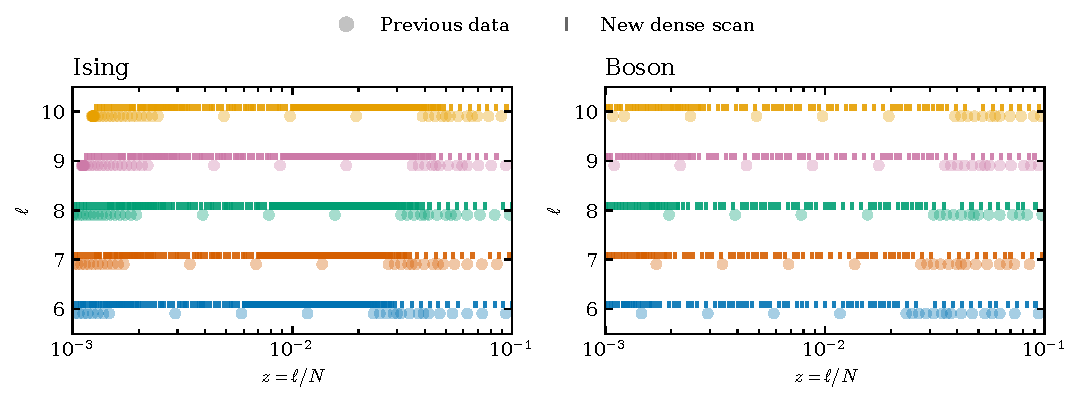
\includegraphics[width=.97\linewidth]{../figs/dense_sampling.pdf}
\caption{Sampling between $10^{-3}$ and $10^{-1}$, common to both interval observables. Circles are the geometries preceding the dense study; vertical marks include the original dense scan and the subsequent fixed-window refinement in Appendix~\ref{sec:common-window-results}. Colors identify $\ell=6,\ldots,10$. Both added grids were chosen from geometry, before their entropies were evaluated, and preserve the largest tested sizes.}
\label{fig:dense-sampling}
\end{figure}

\begin{figure}[!htbp]\centering
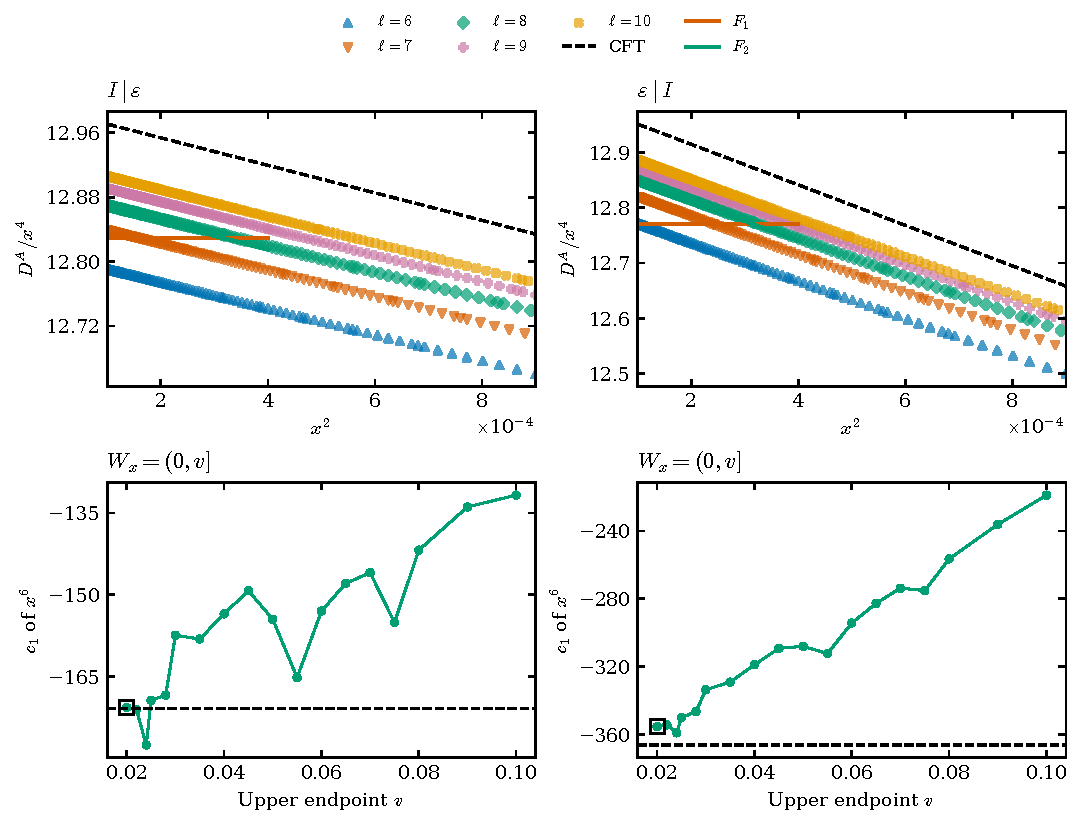
\includegraphics[width=.97\linewidth]{../figs/dense_known_ising.pdf}
\caption{Direct test of the two known Ising second-order coefficients at $p=1/2$. Top: the normalization in Eq.~\eqref{eq:dense-normalized-curve}, zoomed to $0.01\leq x\leq0.03$ with $\ell=6,\ldots,10$, to resolve the fitted slope and the offsets between lengths. The black dashed line is Eq.~\eqref{eq:dense-known-ising}; the fitted lines are drawn only on their actual windows. Bottom: the inferred $x^6$ coefficient as the upper endpoint varies while the displayed lower endpoint stays fixed. Squares mark the reported windows. $I\mid \varepsilon$: $W_x=(0,0.02]$, $m=1255$, $c_0=12.883$, $c_1=-170.71$; $\varepsilon\mid I$: $W_x=(0,0.02]$, $m=1255$, $c_0=12.882$, $c_1=-355.38$. Both $F_2$ coefficients are free; the objective is in $D^A$, not in $D^A/x^4$.}
\label{fig:dense-known}
\end{figure}

\begin{figure}[!htbp]\centering
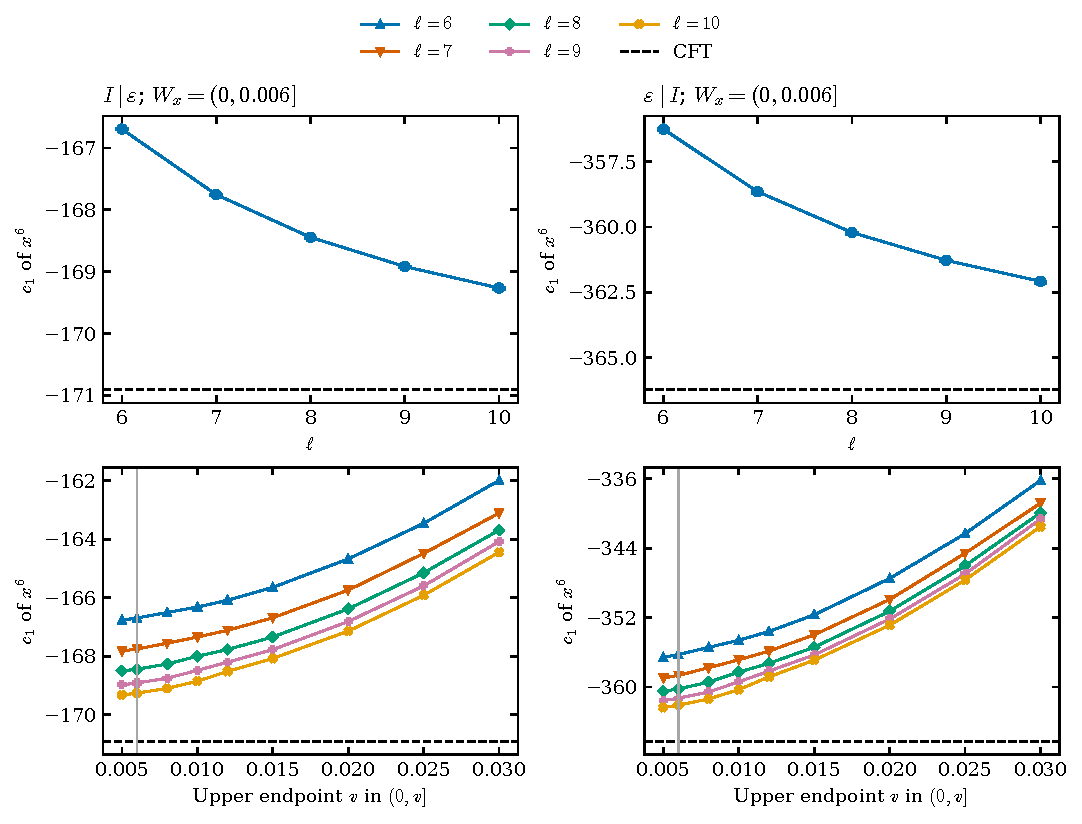
\includegraphics[width=.97\linewidth]{../figs/dense_fixed_subsystem.pdf}
\caption{The same two-power Ising fit performed separately at each subsystem length. Both $x^4$ and $x^6$ coefficients are fitted freely with their exponents fixed; no lattice-correction term is added. Top: vertical bars are the range of $c_1$ across omitted-size refits, not statistical confidence intervals; the marker is the full-data estimate. The black dashed values are Eq.~\eqref{eq:dense-known-ising}. Bottom: coefficient drift as the upper endpoint varies, with each length fitted independently; the vertical line marks the tabulated window. Every fit and every omitted-size training set contains at least forty points. Table~\ref{tab:dense-subsystem} gives the exact counts, both coefficients, and discrepancies.}
\label{fig:dense-subsystem}
\end{figure}

\begin{figure}[!htbp]\centering
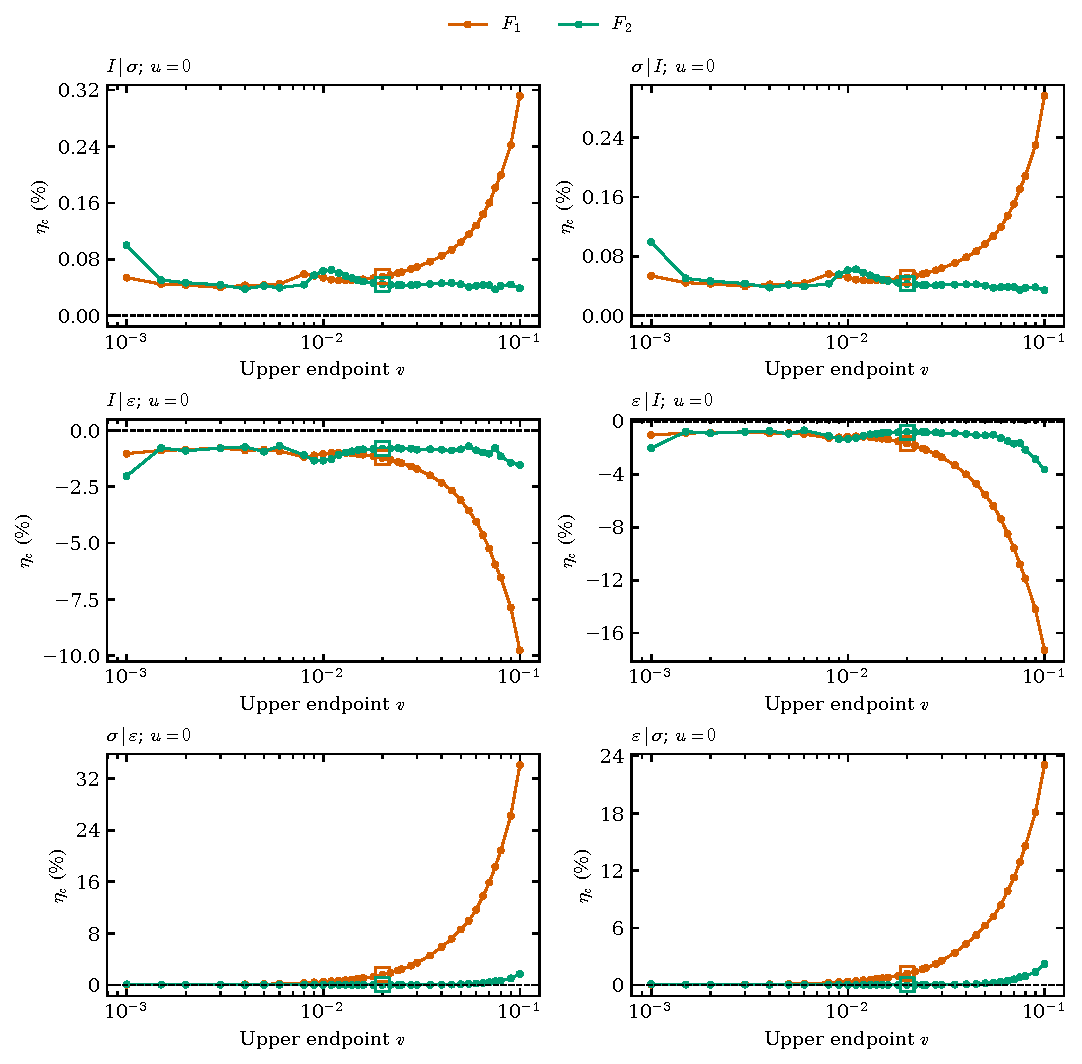
\includegraphics[width=.97\linewidth]{../figs/dense_coefficients_small_ising.pdf}
\caption{Ising small intervals: leading-coefficient discrepancy $\eta_c$ against the upper endpoint $v\leq0.1$ of $W=[u,v]$. Each panel states its fixed $u$; only windows with at least forty points in every omitted-size training set are shown. $F_1$ and $F_2$ always use identical points; $F_2$ fixes both manuscript powers. Squares mark the principal-table windows. All ordinates are linear. The zero line is the theoretical leading coefficient, with its full power of $\pi$.}
\label{fig:dense-coefficients-small-ising}
\end{figure}

\begin{figure}[!htbp]\centering
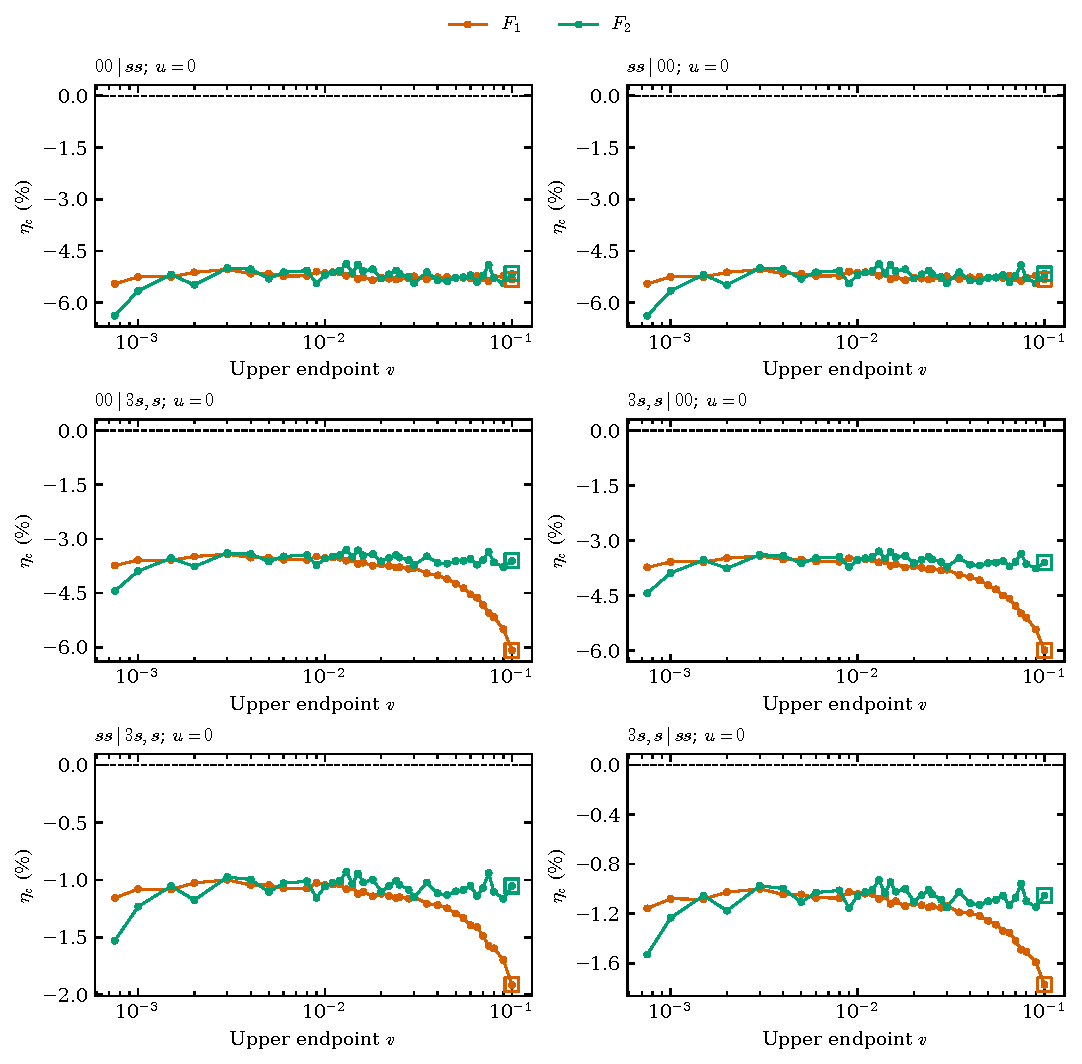
\includegraphics[width=.97\linewidth]{../figs/dense_coefficients_small_boson.pdf}
\caption{Compact boson small intervals: leading-coefficient discrepancy $\eta_c$ against the upper endpoint $v\leq0.1$ of $W=[u,v]$. Each panel states its fixed $u$; only windows with at least forty points in every omitted-size training set are shown. $F_1$ and $F_2$ always use identical points; $F_2$ fixes both manuscript powers. Squares mark the principal-table windows. All ordinates are linear. The zero line is the theoretical leading coefficient, with its full power of $\pi$.}
\label{fig:dense-coefficients-small-boson}
\end{figure}

\begin{figure}[!htbp]\centering
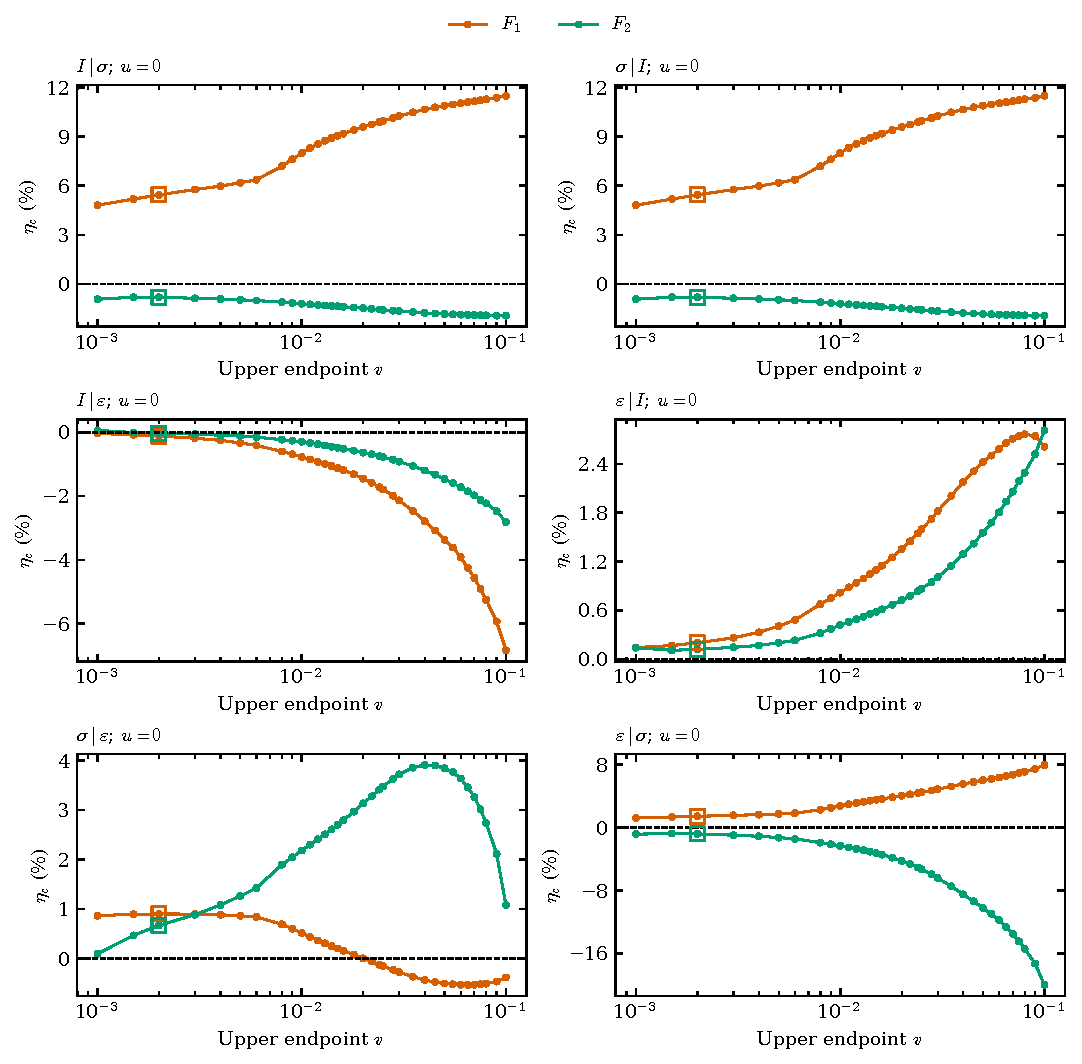
\includegraphics[width=.97\linewidth]{../figs/dense_coefficients_large_ising.pdf}
\caption{Ising large intervals: leading-coefficient discrepancy $\eta_c$ against the upper endpoint $v\leq0.1$ of $W=[u,v]$. Each panel states its fixed $u$; only windows with at least forty points in every omitted-size training set are shown. $F_1$ and $F_2$ always use identical points; $F_2$ fixes both manuscript powers. Squares mark the principal-table windows. All ordinates are linear. The zero line is the theoretical leading coefficient, with its full power of $\pi$.}
\label{fig:dense-coefficients-large-ising}
\end{figure}

\begin{figure}[!htbp]\centering
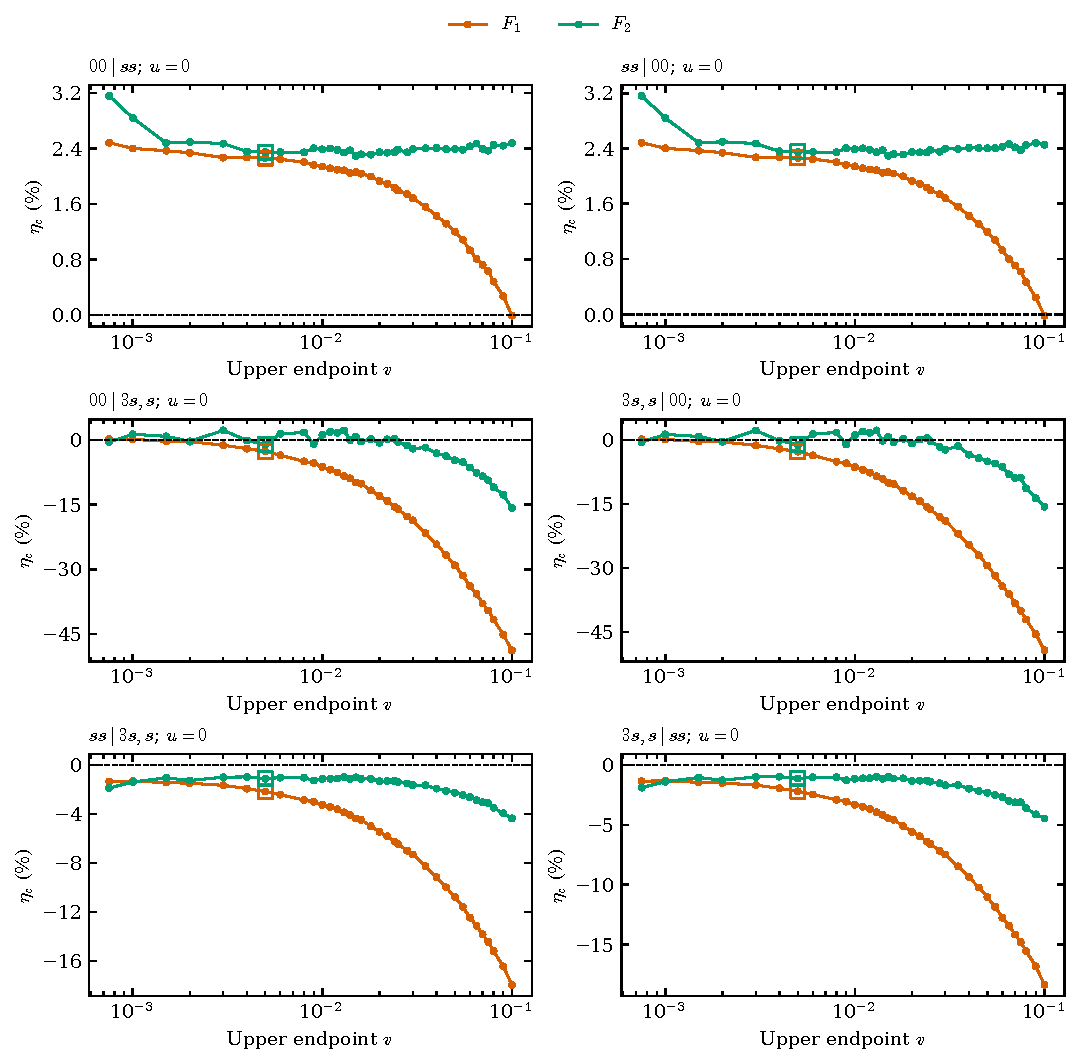
\includegraphics[width=.97\linewidth]{../figs/dense_coefficients_large_boson.pdf}
\caption{Compact boson large intervals: leading-coefficient discrepancy $\eta_c$ against the upper endpoint $v\leq0.1$ of $W=[u,v]$. Each panel states its fixed $u$; only windows with at least forty points in every omitted-size training set are shown. $F_1$ and $F_2$ always use identical points; $F_2$ fixes both manuscript powers. Squares mark the principal-table windows. All ordinates are linear. The zero line is the theoretical leading coefficient, with its full power of $\pi$.}
\label{fig:dense-coefficients-large-boson}
\end{figure}

\begin{figure}[!htbp]\centering
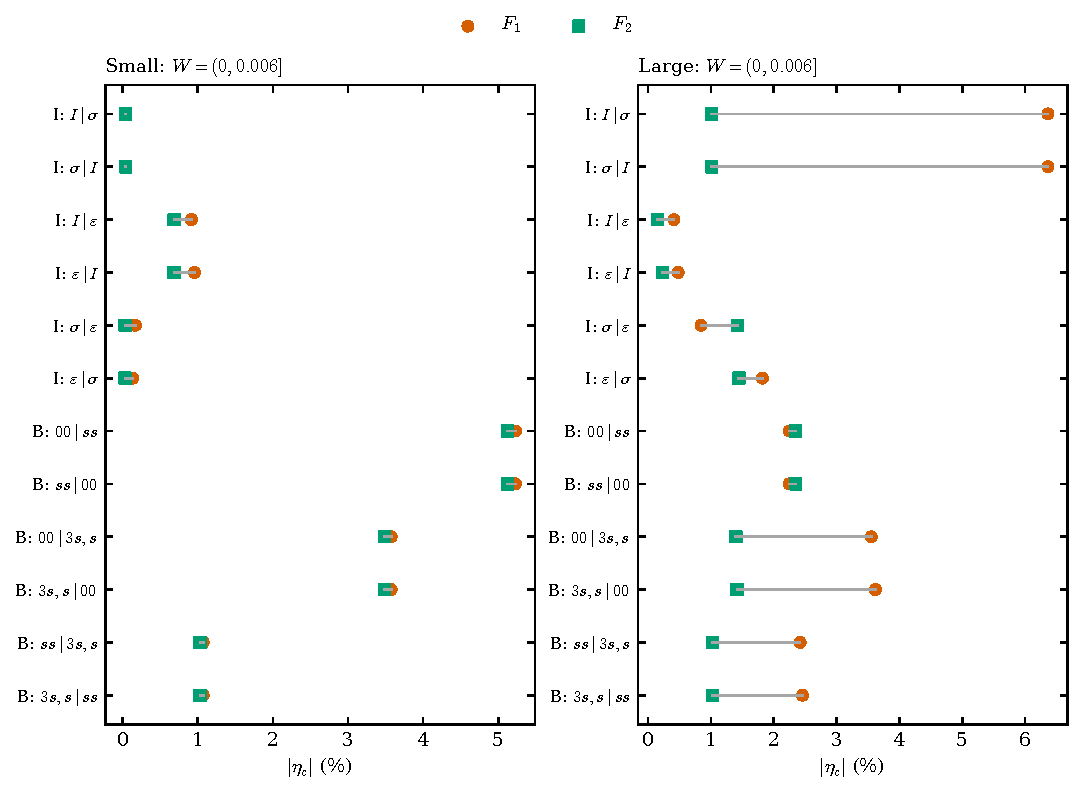
\includegraphics[width=.97\linewidth]{../figs/dense_shared_window.pdf}
\caption{A separate single-window diagnostic across all ordered pairs, using the current enlarged data and distinct from the adopted CFT-specific windows in Eq.~\eqref{eq:common-fit-windows}. I and B identify Ising and compact boson. A leftward shift from the circle ($F_1$) to the square ($F_2$) improves the leading coefficient. The same displayed interval and the same observations are used for both models; powers are fixed to the pair-specific manuscript values. Coefficients include powers of $\pi$, and $|\eta_c|$ is the absolute percentage discrepancy in Eq.~\eqref{eq:metrics}. The original largest sizes and $\ell=6,\ldots,10$ are retained.}
\label{fig:dense-shared}
\end{figure}

\subsection{Matched-window results and reproduction}
The source \path{src/conformal_blocks/dense_windows.py} regenerates
the scan and matched-window comparisons from completed CSVs.
The portable \path{fitting_datas} notebook includes per-model window
controls and the complete scan, selected comparisons, and omitted-size
records. Its defaults keep all models and directions in each CFT and
interval group on the same window. Separate-length and shared-window
figures are explicitly identified diagnostics.
\begingroup\footnotesize
\begingroup\setlength{\tabcolsep}{2pt}
\begin{longtable}{llrrrrrrrr}
\caption{Ising small intervals: identical-window coefficient comparison at $p=1/2$, $\ell=6,\ldots,10$. The displayed $W$ contains $m$ observations. $c_0$ multiplies the leading power and $c_1$ the second manuscript power; both include powers of $\pi$. The column $\Delta_0$ is Eq.~\eqref{eq:dense-coefficient-gain}, in percentage points; $G_{\rm CV}$ is the omitted-size residual gain in Eq.~\eqref{eq:cv}. Positive values mean improvement, but the two measures test different properties. Blank analytical second coefficients are unavailable. Powers and all model parameters are listed in Table~\ref{tab:ising-small-parameters}.}
\label{tab:dense-small-ising}\\\toprule
Direction & $W$ & $m$ & $c_0(F_1)$ & $c_0(F_2)$ & $c_0^{\rm CFT}$ & $c_1(F_2)$ & $c_1^{\rm CFT}$ & $\Delta_0$ & $G_{\rm CV}$\\\midrule
\endfirsthead
\toprule
Direction & $W$ & $m$ & $c_0(F_1)$ & $c_0(F_2)$ & $c_0^{\rm CFT}$ & $c_1(F_2)$ & $c_1^{\rm CFT}$ & $\Delta_0$ & $G_{\rm CV}$\\\midrule
\endhead
\bottomrule\endfoot
$I\mid \sigma$ & $(0,0.02]$ & 1255 & 0.20573 & 0.20571 & 0.20562 & 0.083833 &  & 0.010494 & 2.077\\
$\sigma\mid I$ & $(0,0.02]$ & 1255 & 0.20572 & 0.2057 & 0.20562 & 0.069099 &  & 0.0086493 & 1.8149\\
$I\mid \varepsilon$ & $(0,0.02]$ & 1255 & 12.83 & 12.883 & 12.988 & -170.71 & -170.91 & 0.41412 & 3.8386\\
$\varepsilon\mid I$ & $(0,0.02]$ & 1255 & 12.77 & 12.882 & 12.988 & -355.38 & -366.24 & 0.86214 & 15.195\\
$\sigma\mid \varepsilon$ & $(0,0.02]$ & 1255 & 0.2089 & 0.20565 & 0.20562 & 12.604 &  & 1.5777 & 95.461\\
$\varepsilon\mid \sigma$ & $(0,0.02]$ & 1255 & 0.20806 & 0.20566 & 0.20562 & 9.3133 &  & 1.1658 & 94.318\\
\end{longtable}
\endgroup

\begingroup\setlength{\tabcolsep}{3pt}
\begin{longtable}{llrrrrrr}
\caption{Ising small intervals: second-coefficient sensitivity for Table~\ref{tab:dense-small-ising}. The extrema $c_{1,\min}^{(-N)},c_{1,\max}^{(-N)}$ come from the omitted-size refits and are not confidence bounds. $\eta_1=100(c_1/c_1^{\rm CFT}-1)$ is blank when theory supplies no coefficient. The final column is $100|c_1v^{r_1-r_0}/c_0|$, the size of the fitted second term relative to the first at the window upper endpoint $v$. A fitted nonzero coefficient is not by itself proof of a continuum coefficient.}
\label{tab:dense-small-ising-second}\\\toprule
Direction & $W$ & $c_1$ & $c_1^{\rm CFT}$ & $c_{1,\min}^{(-N)}$ & $c_{1,\max}^{(-N)}$ & $\eta_1$ [\%] & Term ratio [\%]\\\midrule
\endfirsthead
\toprule
Direction & $W$ & $c_1$ & $c_1^{\rm CFT}$ & $c_{1,\min}^{(-N)}$ & $c_{1,\max}^{(-N)}$ & $\eta_1$ [\%] & Term ratio [\%]\\\midrule
\endhead
\bottomrule\endfoot
$I\mid \sigma$ & $(0,0.02]$ & 0.083833 &  & 0.076713 & 0.089011 &  & 0.016301\\
$\sigma\mid I$ & $(0,0.02]$ & 0.069099 &  & 0.063043 & 0.073541 &  & 0.013436\\
$I\mid \varepsilon$ & $(0,0.02]$ & -170.71 & -170.91 & -181.53 & -153.57 & -0.12193 & 0.53\\
$\varepsilon\mid I$ & $(0,0.02]$ & -355.38 & -366.24 & -366.12 & -338.45 & -2.9657 & 1.1035\\
$\sigma\mid \varepsilon$ & $(0,0.02]$ & 12.604 &  & 12.595 & 12.619 &  & 2.4516\\
$\varepsilon\mid \sigma$ & $(0,0.02]$ & 9.3133 &  & 9.3048 & 9.3273 &  & 1.8114\\
\end{longtable}
\endgroup

\begingroup\setlength{\tabcolsep}{2pt}
\begin{longtable}{llrrrrrrrr}
\caption{Compact boson small intervals: identical-window coefficient comparison at $p=1/2$, $\ell=6,\ldots,10$. The displayed $W$ contains $m$ observations. $c_0$ multiplies the leading power and $c_1$ the second manuscript power; both include powers of $\pi$. The column $\Delta_0$ is Eq.~\eqref{eq:dense-coefficient-gain}, in percentage points; $G_{\rm CV}$ is the omitted-size residual gain in Eq.~\eqref{eq:cv}. Positive values mean improvement, but the two measures test different properties. Blank analytical second coefficients are unavailable. Powers and all model parameters are listed in Table~\ref{tab:boson-small-parameters}.}
\label{tab:dense-small-boson}\\\toprule
Direction & $W$ & $m$ & $c_0(F_1)$ & $c_0(F_2)$ & $c_0^{\rm CFT}$ & $c_1(F_2)$ & $c_1^{\rm CFT}$ & $\Delta_0$ & $G_{\rm CV}$\\\midrule
\endfirsthead
\toprule
Direction & $W$ & $m$ & $c_0(F_1)$ & $c_0(F_2)$ & $c_0^{\rm CFT}$ & $c_1(F_2)$ & $c_1^{\rm CFT}$ & $\Delta_0$ & $G_{\rm CV}$\\\midrule
\endhead
\bottomrule\endfoot
$00\mid ss$ & $(0,0.1]$ & 598 & 0.77866 & 0.77996 & 0.82247 & -0.1917 &  & 0.15793 & -2.5678\\
$ss\mid 00$ & $(0,0.1]$ & 598 & 0.77871 & 0.77995 & 0.82247 & -0.18219 &  & 0.1501 & -2.5842\\
$00\mid 3s,s$ & $(0,0.1]$ & 598 & 3.8623 & 3.964 & 4.1123 & -15.02 &  & 2.4748 & 35.203\\
$3s,s\mid 00$ & $(0,0.1]$ & 598 & 3.8657 & 3.9643 & 4.1123 & -14.541 &  & 2.3959 & 35.866\\
$ss\mid 3s,s$ & $(0,0.1]$ & 598 & 1.6134 & 1.6276 & 1.6449 & -2.0896 &  & 0.86075 & 18.998\\
$3s,s\mid ss$ & $(0,0.1]$ & 598 & 1.6157 & 1.6276 & 1.6449 & -1.7507 &  & 0.72113 & 18.631\\
\end{longtable}
\endgroup

\begingroup\setlength{\tabcolsep}{3pt}
\begin{longtable}{llrrrrrr}
\caption{Compact boson small intervals: second-coefficient sensitivity for Table~\ref{tab:dense-small-boson}. The extrema $c_{1,\min}^{(-N)},c_{1,\max}^{(-N)}$ come from the omitted-size refits and are not confidence bounds. $\eta_1=100(c_1/c_1^{\rm CFT}-1)$ is blank when theory supplies no coefficient. The final column is $100|c_1v^{r_1-r_0}/c_0|$, the size of the fitted second term relative to the first at the window upper endpoint $v$. A fitted nonzero coefficient is not by itself proof of a continuum coefficient.}
\label{tab:dense-small-boson-second}\\\toprule
Direction & $W$ & $c_1$ & $c_1^{\rm CFT}$ & $c_{1,\min}^{(-N)}$ & $c_{1,\max}^{(-N)}$ & $\eta_1$ [\%] & Term ratio [\%]\\\midrule
\endfirsthead
\toprule
Direction & $W$ & $c_1$ & $c_1^{\rm CFT}$ & $c_{1,\min}^{(-N)}$ & $c_{1,\max}^{(-N)}$ & $\eta_1$ [\%] & Term ratio [\%]\\\midrule
\endhead
\bottomrule\endfoot
$00\mid ss$ & $(0,0.1]$ & -0.1917 &  & -0.50151 & 0.1399 &  & 0.24579\\
$ss\mid 00$ & $(0,0.1]$ & -0.18219 &  & -0.4909 & 0.14816 &  & 0.23359\\
$00\mid 3s,s$ & $(0,0.1]$ & -15.02 &  & -16.149 & -13.84 &  & 3.7891\\
$3s,s\mid 00$ & $(0,0.1]$ & -14.541 &  & -15.603 & -13.438 &  & 3.668\\
$ss\mid 3s,s$ & $(0,0.1]$ & -2.0896 &  & -2.3303 & -1.8108 &  & 1.2839\\
$3s,s\mid ss$ & $(0,0.1]$ & -1.7507 &  & -1.9474 & -1.5292 &  & 1.0756\\
\end{longtable}
\endgroup

\begingroup\setlength{\tabcolsep}{2pt}
\begin{longtable}{llrrrrrrrr}
\caption{Ising large intervals: identical-window coefficient comparison at $p=1/2$, $\ell=6,\ldots,10$. The displayed $W$ contains $m$ observations. $c_0$ multiplies the leading power and $c_1$ the second manuscript power; both include powers of $\pi$. The column $\Delta_0$ is Eq.~\eqref{eq:dense-coefficient-gain}, in percentage points; $G_{\rm CV}$ is the omitted-size residual gain in Eq.~\eqref{eq:cv}. Positive values mean improvement, but the two measures test different properties. Blank analytical second coefficients are unavailable. Powers and all model parameters are listed in Table~\ref{tab:ising-large-parameters}.}
\label{tab:dense-large-ising}\\\toprule
Direction & $W$ & $m$ & $c_0(F_1)$ & $c_0(F_2)$ & $c_0^{\rm CFT}$ & $c_1(F_2)$ & $c_1^{\rm CFT}$ & $\Delta_0$ & $G_{\rm CV}$\\\midrule
\endfirsthead
\toprule
Direction & $W$ & $m$ & $c_0(F_1)$ & $c_0(F_2)$ & $c_0^{\rm CFT}$ & $c_1(F_2)$ & $c_1^{\rm CFT}$ & $\Delta_0$ & $G_{\rm CV}$\\\midrule
\endhead
\bottomrule\endfoot
$I\mid \sigma$ & $(0,0.002]$ & 260 & 0.65339 & 0.61463 & 0.61965 & 0.20243 &  & 4.6332 & 96.863\\
$\sigma\mid I$ & $(0,0.002]$ & 260 & 0.65339 & 0.61462 & 0.61965 & 0.20245 &  & 4.6331 & 96.886\\
$I\mid \varepsilon$ & $(0,0.002]$ & 260 & 3.2861 & 3.289 & 3.2899 & -1070.2 &  & 0.090409 & 47.468\\
$\varepsilon\mid I$ & $(0,0.002]$ & 260 & 3.2964 & 3.2938 & 3.2899 & 959.21 &  & 0.081036 & 53.25\\
$\sigma\mid \varepsilon$ & $(0,0.002]$ & 260 & 0.15631 & 0.15595 & 0.15491 & 0.0018716 &  & 0.23133 & 19.238\\
$\varepsilon\mid \sigma$ & $(0,0.002]$ & 260 & 0.15712 & 0.15365 & 0.15491 & 0.018087 &  & 0.60996 & 90.498\\
\end{longtable}
\endgroup

\begingroup\setlength{\tabcolsep}{3pt}
\begin{longtable}{llrrrrrr}
\caption{Ising large intervals: second-coefficient sensitivity for Table~\ref{tab:dense-large-ising}. The extrema $c_{1,\min}^{(-N)},c_{1,\max}^{(-N)}$ come from the omitted-size refits and are not confidence bounds. $\eta_1=100(c_1/c_1^{\rm CFT}-1)$ is blank when theory supplies no coefficient. The final column is $100|c_1v^{r_1-r_0}/c_0|$, the size of the fitted second term relative to the first at the window upper endpoint $v$. A fitted nonzero coefficient is not by itself proof of a continuum coefficient.}
\label{tab:dense-large-ising-second}\\\toprule
Direction & $W$ & $c_1$ & $c_1^{\rm CFT}$ & $c_{1,\min}^{(-N)}$ & $c_{1,\max}^{(-N)}$ & $\eta_1$ [\%] & Term ratio [\%]\\\midrule
\endfirsthead
\toprule
Direction & $W$ & $c_1$ & $c_1^{\rm CFT}$ & $c_{1,\min}^{(-N)}$ & $c_{1,\max}^{(-N)}$ & $\eta_1$ [\%] & Term ratio [\%]\\\midrule
\endhead
\bottomrule\endfoot
$I\mid \sigma$ & $(0,0.002]$ & 0.20243 &  & 0.20232 & 0.20251 &  & 6.9649\\
$\sigma\mid I$ & $(0,0.002]$ & 0.20245 &  & 0.20234 & 0.20253 &  & 6.9657\\
$I\mid \varepsilon$ & $(0,0.002]$ & -1070.2 &  & -1095.7 & -1053.3 &  & 0.13015\\
$\varepsilon\mid I$ & $(0,0.002]$ & 959.21 &  & 944.43 & 976.81 &  & 0.11649\\
$\sigma\mid \varepsilon$ & $(0,0.002]$ & 0.0018716 &  & 0.0018486 & 0.0019195 &  & 0.25379\\
$\varepsilon\mid \sigma$ & $(0,0.002]$ & 0.018087 &  & 0.018053 & 0.01811 &  & 2.4894\\
\end{longtable}
\endgroup

\begingroup\setlength{\tabcolsep}{2pt}
\begin{longtable}{llrrrrrrrr}
\caption{Compact boson large intervals: identical-window coefficient comparison at $p=1/2$, $\ell=6,\ldots,10$. The displayed $W$ contains $m$ observations. $c_0$ multiplies the leading power and $c_1$ the second manuscript power; both include powers of $\pi$. The column $\Delta_0$ is Eq.~\eqref{eq:dense-coefficient-gain}, in percentage points; $G_{\rm CV}$ is the omitted-size residual gain in Eq.~\eqref{eq:cv}. Positive values mean improvement, but the two measures test different properties. Blank analytical second coefficients are unavailable. Powers and all model parameters are listed in Table~\ref{tab:boson-large-parameters}.}
\label{tab:dense-large-boson}\\\toprule
Direction & $W$ & $m$ & $c_0(F_1)$ & $c_0(F_2)$ & $c_0^{\rm CFT}$ & $c_1(F_2)$ & $c_1^{\rm CFT}$ & $\Delta_0$ & $G_{\rm CV}$\\\midrule
\endfirsthead
\toprule
Direction & $W$ & $m$ & $c_0(F_1)$ & $c_0(F_2)$ & $c_0^{\rm CFT}$ & $c_1(F_2)$ & $c_1^{\rm CFT}$ & $\Delta_0$ & $G_{\rm CV}$\\\midrule
\endhead
\bottomrule\endfoot
$00\mid ss$ & $(0,0.005]$ & 317 & 1.2616 & 1.2627 & 1.2337 & -0.33376 &  & -0.085416 & -0.80584\\
$ss\mid 00$ & $(0,0.005]$ & 317 & 1.2616 & 1.2627 & 1.2337 & -0.34138 &  & -0.087364 & -0.7901\\
$00\mid 3s,s$ & $(0,0.005]$ & 317 & 73.093 & 74.307 & 75.109 & -265.58 &  & 1.6153 & -0.40053\\
$3s,s\mid 00$ & $(0,0.005]$ & 317 & 73.058 & 74.252 & 75.109 & -261.18 &  & 1.5885 & -0.47282\\
$ss\mid 3s,s$ & $(0,0.005]$ & 317 & 3.2185 & 3.2529 & 3.2899 & -8.6617 &  & 1.0449 & 13.931\\
$3s,s\mid ss$ & $(0,0.005]$ & 317 & 3.2176 & 3.2528 & 3.2899 & -8.8758 &  & 1.0707 & 13.775\\
\end{longtable}
\endgroup

\begingroup\setlength{\tabcolsep}{3pt}
\begin{longtable}{llrrrrrr}
\caption{Compact boson large intervals: second-coefficient sensitivity for Table~\ref{tab:dense-large-boson}. The extrema $c_{1,\min}^{(-N)},c_{1,\max}^{(-N)}$ come from the omitted-size refits and are not confidence bounds. $\eta_1=100(c_1/c_1^{\rm CFT}-1)$ is blank when theory supplies no coefficient. The final column is $100|c_1v^{r_1-r_0}/c_0|$, the size of the fitted second term relative to the first at the window upper endpoint $v$. A fitted nonzero coefficient is not by itself proof of a continuum coefficient.}
\label{tab:dense-large-boson-second}\\\toprule
Direction & $W$ & $c_1$ & $c_1^{\rm CFT}$ & $c_{1,\min}^{(-N)}$ & $c_{1,\max}^{(-N)}$ & $\eta_1$ [\%] & Term ratio [\%]\\\midrule
\endfirsthead
\toprule
Direction & $W$ & $c_1$ & $c_1^{\rm CFT}$ & $c_{1,\min}^{(-N)}$ & $c_{1,\max}^{(-N)}$ & $\eta_1$ [\%] & Term ratio [\%]\\\midrule
\endhead
\bottomrule\endfoot
$00\mid ss$ & $(0,0.005]$ & -0.33376 &  & -0.53362 & -0.14815 &  & 0.13216\\
$ss\mid 00$ & $(0,0.005]$ & -0.34138 &  & -0.53762 & -0.15672 &  & 0.13518\\
$00\mid 3s,s$ & $(0,0.005]$ & -265.58 &  & -373.74 & -178.05 &  & 1.7871\\
$3s,s\mid 00$ & $(0,0.005]$ & -261.18 &  & -372.89 & -175.63 &  & 1.7588\\
$ss\mid 3s,s$ & $(0,0.005]$ & -8.6617 &  & -9.6333 & -8.0378 &  & 1.3314\\
$3s,s\mid ss$ & $(0,0.005]$ & -8.8758 &  & -9.8805 & -8.2283 &  & 1.3643\\
\end{longtable}
\endgroup

\begingroup\setlength{\tabcolsep}{3pt}
\begin{longtable}{lrrrrrrr}
\caption{Known Ising coefficient checks separated by subsystem length, at $p=1/2$ and the common window $W_x=(0,0.006]$. Each row fits $c_0x^4+c_1x^6$ to the stated $\ell$ only; $m$ counts distinct chain sizes. The theoretical coefficients are Eq.~\eqref{eq:dense-known-ising}; $\eta_j=100(c_j/c_j^{\rm CFT}-1)$, $j=0,1$, are signed percentage discrepancies. The final column gives the extrema from omitting each chain size and refitting. These deterministic ranges are sensitivity measures, not confidence intervals.}
\label{tab:dense-subsystem}\\\toprule
Direction & $\ell$ & $m$ & $c_0$ & $\eta_0$ [\%] & $c_1$ & $\eta_1$ [\%] & $c_1$ omitted-size range\\\midrule
\endfirsthead
\toprule
Direction & $\ell$ & $m$ & $c_0$ & $\eta_0$ [\%] & $c_1$ & $\eta_1$ [\%] & $c_1$ omitted-size range\\\midrule
\endhead
\bottomrule\endfoot
$I\mid \varepsilon$ & 6 & 97 & 12.808 & -1.3871 & -166.69 & -2.4684 & $[-166.71,-166.69]$\\
$I\mid \varepsilon$ & 7 & 92 & 12.855 & -1.0194 & -167.75 & -1.8482 & $[-167.77,-167.75]$\\
$I\mid \varepsilon$ & 8 & 89 & 12.886 & -0.78063 & -168.45 & -1.4442 & $[-168.47,-168.44]$\\
$I\mid \varepsilon$ & 9 & 86 & 12.908 & -0.61689 & -168.92 & -1.1677 & $[-168.93,-168.92]$\\
$I\mid \varepsilon$ & 10 & 82 & 12.923 & -0.49974 & -169.27 & -0.96408 & $[-169.28,-169.26]$\\
$\varepsilon\mid I$ & 6 & 97 & 12.808 & -1.3872 & -356.25 & -2.7295 & $[-356.3,-356.24]$\\
$\varepsilon\mid I$ & 7 & 92 & 12.855 & -1.0194 & -358.64 & -2.075 & $[-358.73,-358.64]$\\
$\varepsilon\mid I$ & 8 & 89 & 12.886 & -0.78069 & -360.21 & -1.6477 & $[-360.3,-360.2]$\\
$\varepsilon\mid I$ & 9 & 86 & 12.908 & -0.61696 & -361.28 & -1.3561 & $[-361.32,-361.27]$\\
$\varepsilon\mid I$ & 10 & 82 & 12.923 & -0.4998 & -362.08 & -1.1357 & $[-362.16,-362.08]$\\
\end{longtable}
\endgroup

\endgroup

\clearpage
\subsection{Zero-anchored common windows on the denser data}
\label{sec:common-window-results}
The small-Ising and small-boson windows remain $(0,0.02]$ and
$(0,0.1]$. The large-interval comparison adopts $(0,0.002]$ for Ising
and the prescribed $(0,0.005]$ for the compact boson. These are the
four windows of Eq.~\eqref{eq:common-fit-windows}; every model and
all six directions within each group use identical observations.
The preceding data refinement added 48 even system sizes for each CFT, with all five
lengths $\ell=6,7,8,9,10$ at each size. The largest sizes remain
$8192$ and $16384$. Every added geometry enters the corresponding
small-interval window; only those satisfying the separate large-interval
cutoff enter its fits. Both observables are computed and preserved.
The data refinement initially kept all four windows fixed. A subsequent
zero-anchored search selected the historical large-boson cutoff $0.0047$.
The current revision changes that cutoff to the prescribed $0.005$,
on exactly the same raw data. All theoretical powers are unchanged.
At the current cutoff, $F_2$ improves four of the six large-boson
leading coefficients; the all-six target is not met.

The new sizes are chosen using geometry alone. For each CFT, seed
the even sizes at which each length first enters its large-interval
window. Repeatedly bisect the largest gap in $\log N$, choosing the
nearest unused even size to the geometric midpoint. Add 32 sizes
in $3000\leq N\leq8192$ for Ising or $3750\leq N\leq16384$ for
the boson. Add 16 further sizes in $500\leq N\leq3000$ or
$100\leq N\leq3750$, respectively. Existing sizes are never
recomputed or replaced. The exact executed lists are included in
Eq.~\eqref{eq:extended-grid} and the data manifest below.

Table~\ref{tab:common-window-counts} gives the updated counts. On the adopted windows, $F_2$ improves the absolute leading-coefficient discrepancy in 22 of 24 cases and omitted-size prediction in 18 of 24 cases. All models use the same observations within each group. The current large-boson cutoff is prescribed as $0.005$; the earlier coefficient-guided choice $0.0047$ is retained as a historical comparison.

The added sizes pass all 10512 stored production checks of the types in Table~\ref{tab:scaling-numerical-checks}. Recomputing 450 directed rows from saved matrices reproduces every recorded value exactly. No entropy calculation or physical observation is changed by this window revision.

The two small-interval windows and all their coefficients are unchanged from the denser-data revision. The known Ising $x^6$ coefficients and their discrepancies are given in Tables~\ref{tab:dense-small-ising} and \ref{tab:dense-small-ising-second}.

\begingroup\footnotesize
\begingroup\setlength{\tabcolsep}{3pt}
\begin{longtable}{lllrrrrr}
\caption{Adopted common-window results for $p=1/2$, $\ell=6,\ldots,10$. Counts apply to every direction. The last two columns count directions with positive leading-coefficient gain $\Delta_0$ in Eq.~\eqref{eq:dense-coefficient-gain} and positive omitted-size prediction gain $G_{\rm CV}$ in Eq.~\eqref{eq:cv}, respectively. All three fitted models use the stated window. The large-boson upper cutoff is prescribed as $0.005$.}
\label{tab:common-window-counts}\\\toprule
Interval & CFT & $W$ & $m$ & Sizes & Min. training & $\Delta_0>0$ & $G_{\rm CV}>0$\\\midrule
\endfirsthead
\toprule
Interval & CFT & $W$ & $m$ & Sizes & Min. training & $\Delta_0>0$ & $G_{\rm CV}>0$\\\midrule
\endhead
\bottomrule\endfoot
small & ising & $(0,0.02]$ & 1255 & 278 & 1250 & 6/6 & 6/6\\
small & boson & $(0,0.1]$ & 598 & 124 & 593 & 6/6 & 4/6\\
large & ising & $(0,0.002]$ & 260 & 67 & 255 & 6/6 & 6/6\\
large & boson & $(0,0.005]$ & 317 & 68 & 312 & 4/6 & 2/6\\
\end{longtable}
\endgroup

\endgroup

For large Ising, the adopted window retains 260 observations per direction at 67 distinct chain sizes. Relative to $F_1$ on those observations, $F_2$ improves the leading coefficient in 6 of six directions and omitted-size prediction in 6 of six. The coefficient gain stays positive in every omitted-size refit for 6 directions. Table~\ref{tab:common-large-ising} compares with the preceding report window on the same numerical grid.

\begingroup\footnotesize
\begingroup\setlength{\tabcolsep}{3pt}
\begin{longtable}{lrrrrr}
\caption{Ising large intervals: absolute leading-coefficient discrepancies $E_0=|\eta_c|$, with $\eta_c$ defined in Eq.~\eqref{eq:metrics}. Both versions use the same numerical grid. The previous $F_2$ column uses $(0,0.002]$ with 260 observations per direction; the current fits use $(0,0.002]$ with 260. $G_{\rm CV}$ compares $F_2$ with $F_1$ on the same current window and observations. The last column counts omitted-size refits in which $\Delta_0>0$. All discrepancies and gains are percentages; these are deterministic comparisons, not statistical error bars.}
\label{tab:common-large-ising}\\\toprule
Direction & $E_0(F_1)$ & $E_0(F_2)$ & Previous $E_0(F_2)$ & $G_{\rm CV}$ & Positive folds\\\midrule
\endfirsthead
\toprule
Direction & $E_0(F_1)$ & $E_0(F_2)$ & Previous $E_0(F_2)$ & $G_{\rm CV}$ & Positive folds\\\midrule
\endhead
\bottomrule\endfoot
$I\mid \sigma$ & 5.4442 & 0.81098 & 0.81098 & 96.863 & 67/67\\
$\sigma\mid I$ & 5.4445 & 0.81139 & 0.81139 & 96.886 & 67/67\\
$I\mid \varepsilon$ & 0.11533 & 0.024918 & 0.024918 & 47.468 & 67/67\\
$\varepsilon\mid I$ & 0.19921 & 0.11818 & 0.11818 & 53.25 & 67/67\\
$\sigma\mid \varepsilon$ & 0.9017 & 0.67037 & 0.67037 & 19.238 & 67/67\\
$\varepsilon\mid \sigma$ & 1.4228 & 0.81285 & 0.81285 & 90.498 & 67/67\\
\end{longtable}
\endgroup

\endgroup

For large compact boson, the adopted window retains 317 observations per direction at 68 distinct chain sizes. Relative to $F_1$ on those observations, $F_2$ improves the leading coefficient in 4 of six directions and omitted-size prediction in 2 of six. The coefficient gain stays positive in every omitted-size refit for 4 directions. Table~\ref{tab:common-large-boson} compares with the preceding report window on the same numerical grid.

$00\mid ss$ has absolute leading discrepancies $2.2645\%$ under $F_1$ and $2.34992\%$ under $F_2$. Its omitted-size prediction gain is $-0.805838\%$, and the leading gain stays positive in 0 of 68 refits. Negative prediction gains denote worse prediction.

$ss\mid 00$ has absolute leading discrepancies $2.26363\%$ under $F_1$ and $2.351\%$ under $F_2$. Its omitted-size prediction gain is $-0.790097\%$, and the leading gain stays positive in 0 of 68 refits. Negative prediction gains denote worse prediction.

$00\mid 3s,s$ has absolute leading discrepancies $2.68291\%$ under $F_1$ and $1.06764\%$ under $F_2$. Its omitted-size prediction gain is $-0.400526\%$, and the leading gain stays positive in 68 of 68 refits. Negative prediction gains denote worse prediction.

$3s,s\mid 00$ has absolute leading discrepancies $2.72951\%$ under $F_1$ and $1.14099\%$ under $F_2$. Its omitted-size prediction gain is $-0.47282\%$, and the leading gain stays positive in 68 of 68 refits. Negative prediction gains denote worse prediction.

\begingroup\footnotesize
\begingroup\setlength{\tabcolsep}{3pt}
\begin{longtable}{lrrrrr}
\caption{Compact boson large intervals: absolute leading-coefficient discrepancies $E_0=|\eta_c|$, with $\eta_c$ defined in Eq.~\eqref{eq:metrics}. Both versions use the same numerical grid. The previous $F_2$ column uses $(0,0.0047]$ with 311 observations per direction; the current fits use $(0,0.005]$ with 317. $G_{\rm CV}$ compares $F_2$ with $F_1$ on the same current window and observations. The last column counts omitted-size refits in which $\Delta_0>0$. All discrepancies and gains are percentages; these are deterministic comparisons, not statistical error bars.}
\label{tab:common-large-boson}\\\toprule
Direction & $E_0(F_1)$ & $E_0(F_2)$ & Previous $E_0(F_2)$ & $G_{\rm CV}$ & Positive folds\\\midrule
\endfirsthead
\toprule
Direction & $E_0(F_1)$ & $E_0(F_2)$ & Previous $E_0(F_2)$ & $G_{\rm CV}$ & Positive folds\\\midrule
\endhead
\bottomrule\endfoot
$00\mid ss$ & 2.2645 & 2.3499 & 2.2855 & -0.80584 & 0/68\\
$ss\mid 00$ & 2.2636 & 2.351 & 2.2855 & -0.7901 & 0/68\\
$00\mid 3s,s$ & 2.6829 & 1.0676 & 2.197 & -0.40053 & 68/68\\
$3s,s\mid 00$ & 2.7295 & 1.141 & 2.2251 & -0.47282 & 68/68\\
$ss\mid 3s,s$ & 2.1683 & 1.1234 & 0.8515 & 13.931 & 68/68\\
$3s,s\mid ss$ & 2.1982 & 1.1274 & 0.84555 & 13.775 & 68/68\\
\end{longtable}
\endgroup

\clearpage
\begingroup\setlength{\tabcolsep}{4pt}
\begin{longtable}{lrrrrr}
\caption{Concrete neighboring-cutoff tests for the large intervals. Every row uses $W_y=(0,v]$ for all directions, both fitted powers fixed as in Table~\ref{tab:complement-theory}, and $\ell=6,\ldots,10$. The two count columns use the definitions in Table~\ref{tab:common-window-counts}. The last column is the largest absolute leading-coefficient discrepancy among the six $F_2$ fits, in percent. The changing $m$ shows when a cutoff adds an actual observation.}
\label{tab:common-window-neighbors}\\\toprule
CFT & $v$ & $m$ & $\Delta_0>0$ & $G_{\rm CV}>0$ & Max. $E_0(F_2)$\\\midrule
\endfirsthead
\toprule
CFT & $v$ & $m$ & $\Delta_0>0$ & $G_{\rm CV}>0$ & Max. $E_0(F_2)$\\\midrule
\endhead
\bottomrule\endfoot
ising & 0.0015 & 175 & 6/6 & 6/6 & 0.80928\\
ising & 0.002 & 260 & 6/6 & 6/6 & 0.81285\\
ising & 0.0025 & 314 & 6/6 & 6/6 & 0.90129\\
ising & 0.003 & 348 & 6/6 & 5/6 & 0.97471\\
ising & 0.004 & 389 & 5/6 & 6/6 & 1.1168\\
boson & 0.0016 & 193 & 2/6 & 2/6 & 2.4537\\
boson & 0.0045 & 308 & 4/6 & 4/6 & 2.3172\\
boson & 0.0046 & 308 & 4/6 & 4/6 & 2.3172\\
boson & 0.00465 & 310 & 4/6 & 4/6 & 2.3126\\
boson & 0.00469 & 310 & 4/6 & 4/6 & 2.3126\\
boson & 0.0047 & 311 & 6/6 & 4/6 & 2.2855\\
boson & 0.00472 & 311 & 6/6 & 4/6 & 2.2855\\
boson & 0.00474 & 311 & 6/6 & 4/6 & 2.2855\\
boson & 0.00475 & 312 & 4/6 & 4/6 & 2.2959\\
boson & 0.0048 & 313 & 4/6 & 2/6 & 2.3298\\
boson & 0.0049 & 315 & 4/6 & 2/6 & 2.3732\\
boson & 0.005 & 317 & 4/6 & 2/6 & 2.351\\
\end{longtable}
\endgroup

\endgroup

The zero-anchored search on the current grid enumerates every distinct selection $W_y=(0,v]$ through $v=0.20$, requiring at least forty observations after omitting any chain size. It contains 1361 admissible Ising windows and 532 boson windows. Of the Ising windows, 258 improve all six leading estimates and 251 also improve omitted-size prediction in all six directions. The already adopted Ising cutoff remains suitable.

For the boson, exactly one distinct data selection improves all six leading estimates. The corresponding upper cutoffs satisfy \begin{equation}0.004691689008042895\leq v<0.004741833508956797.\label{eq:zero-equivalent-cutoffs}\end{equation} The rounded value $v=0.0047$ lies in this range. The existing endpoint comparison tolerance is $10^{-14}$. There are no observations between the bounding fractions, so changing $v$ inside this range does not provide a new sampling test.

Table~\ref{tab:common-window-neighbors} retains the neighboring failures. The historical all-six coefficient gain at $0.0047$ disappears at the immediately adjacent selections; its weakest gain, for $ss\mid00$, is only about $0.00555$ percentage points. No enumerated zero-anchored boson window improves both coefficient accuracy and omitted-size prediction in all six directions. Figures~\ref{fig:zero-anchored-scan} and \ref{fig:zero-anchored-zoom} show this cutoff dependence. The currently prescribed window $0<y\leq0.005$ has 317 observations per direction and improves 4 of six leading coefficients; it does not meet the all-six target.

The earlier exhaustive search on 23472 observations and the subsequent fixed-window density comparison remain historical records. Their windows and conclusions must not be substituted for this search on the enlarged grid. All physical data are preserved; only derived selection flags and fitted summaries change in this revision.

\begin{sloppypar}The current directed results are in \path{data/common_cft_coefficient_comparison.csv}; \path{data/zero_adoption_cv.csv} and \path{data/zero_neighbor_cv.csv} retain the omitted-size fits. Files prefixed \texttt{zero\_anchored\_} contain the exhaustive scan and its validation; files prefixed \texttt{zero\_before\_} preserve the preceding report. The portable \path{fitting_datas} notebook uses the same adopted windows and refitted coefficients. The two cutoff figures have linear discrepancy ordinates.\end{sloppypar}

\clearpage
\begin{figure}[p]
\centering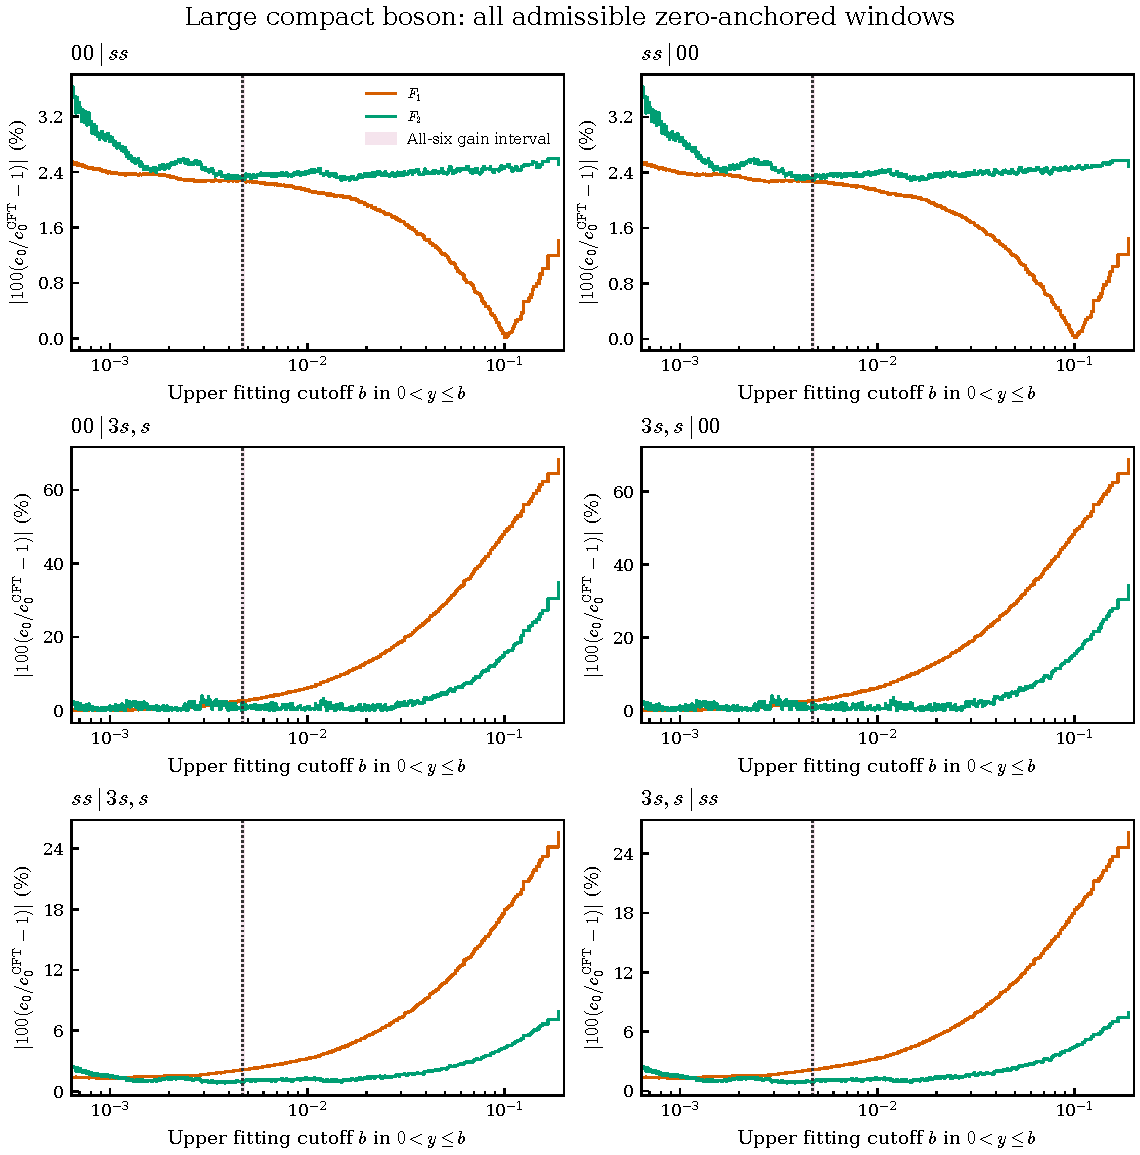
\includegraphics[width=\textwidth,height=.83\textheight,keepaspectratio]{../figs/zero_anchored_cutoff_scan.pdf}
\caption{Large-boson leading-coefficient accuracy across all admissible zero-anchored windows $W_y=(0,v]$ through $v=0.20$, using $p=1/2$ and $\ell=6,7,8,9,10$. The plotting symbol $b$ on the horizontal axis denotes the trial upper cutoff $v$, not a primary-state label. Each step corresponds to a distinct selected data set with at least forty training observations after any chain-size omission. Both powers of $F_2$ are fixed to Table~\ref{tab:complement-theory}; $F_1$ uses only its leading power. The ordinate is $|\eta_c|$ from Eq.~\eqref{eq:metrics}, on a linear scale. The dotted line marks the previous candidate $v=0.0047$, and the shaded band marks Eq.~\eqref{eq:zero-equivalent-cutoffs}. The current prescribed cutoff is $0.005$; its counts and minimum training sizes are in Table~\ref{tab:common-window-counts}.}
\label{fig:zero-anchored-scan}
\end{figure}
\clearpage
\begin{figure}[p]
\centering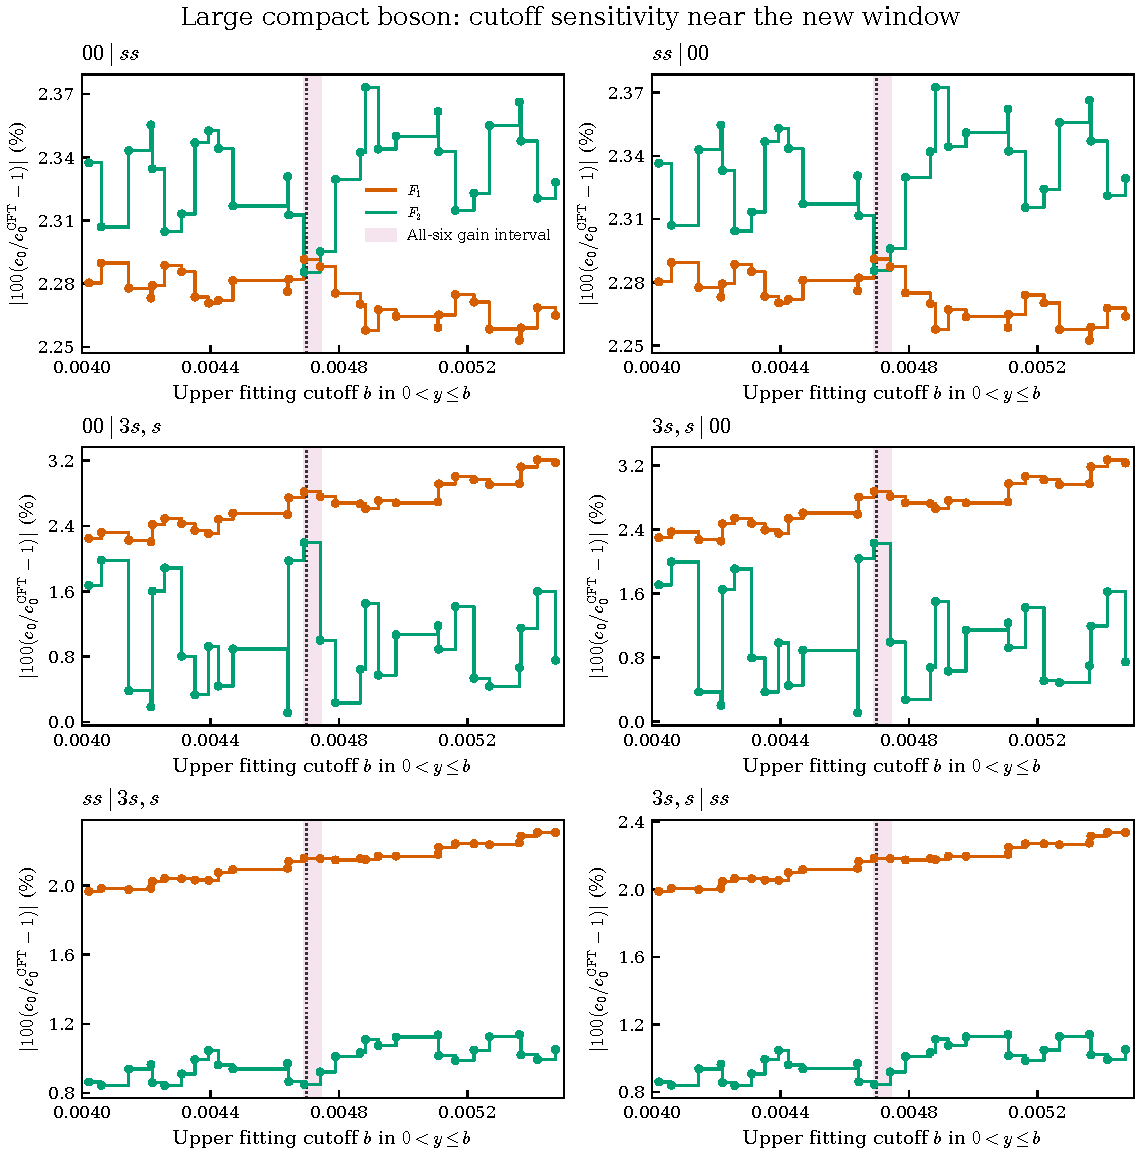
\includegraphics[width=\textwidth,height=.83\textheight,keepaspectratio]{../figs/zero_anchored_cutoff_zoom.pdf}
\caption{Historical cutoff sensitivity around the previous large-boson candidate $0.0047$, using the same data, models and discrepancy as Fig.~\ref{fig:zero-anchored-scan}. Markers show actual changes of data membership; both axes are linear. The shaded historical interval has 311 points per direction from 68 chain sizes. The nearest selections outside it lose the all-six leading-coefficient gain, as quantified in Table~\ref{tab:common-window-neighbors}. The residual reduction alone does not establish coefficient recovery.}
\label{fig:zero-anchored-zoom}
\end{figure}
\clearpage



\begin{thebibliography}{99}
\raggedright
\small
\bibitem{GolubPereyra} G. H. Golub and V. Pereyra,
\emph{The differentiation of pseudo-inverses and nonlinear least
squares problems whose variables separate}, SIAM J. Numer. Anal.
\textbf{10}(2), 413--432 (1973),
\href{https://doi.org/10.1137/0710036}{doi:10.1137/0710036}.
\bibitem{theoryLarge} N. Lashkari and J. Mohanty,
\emph{Relative entropy of mixtures of excited states in CFT},
supplied working manuscript \texttt{manuscript\_theory/main3.tex}.
The large-interval two-point result and the subsections on Ising and
non-chiral compact-boson examples are used here. The accompanying
\texttt{main.pdf} is an older version and does not contain those examples.
\bibitem{Bravyi} S. Bravyi,
\emph{Lagrangian representation for fermionic linear optics},
Quantum Inf. Comput. \textbf{5}, 216--238 (2005),
\href{https://arxiv.org/abs/quant-ph/0404180}{arXiv:quant-ph/0404180}.
\bibitem{Surace} J. Surace and L. Tagliacozzo,
\emph{Fermionic Gaussian states: an introduction to numerical approaches},
\href{https://arxiv.org/abs/2111.08343}{arXiv:2111.08343}.
\bibitem{theory} Supplied manuscript, \emph{Relative entropy of mixtures},
PDF and source archive in \texttt{Theory\_paper/}; matching discussion
in \texttt{main3.tex}, Sec.~4.2, Eqs.~(4.13)--(4.18). The six boson pairs
are specified explicitly in the user's request; table numbering differs
between manuscript versions.
\bibitem{Herwerth} B. Herwerth, G. Sierra, H.-H. Tu, and A. E. B. Nielsen,
\emph{Excited states in spin chains from conformal blocks},
Phys. Rev. B \textbf{91}, 235121 (2015),
\href{https://arxiv.org/abs/1501.07557}{arXiv:1501.07557}.
\bibitem{Montes2016} S. Montes, J. Rodr\'{i}guez-Laguna, H.-H. Tu, and G. Sierra,
\emph{Many-body lattice wavefunctions from conformal blocks},
Phys. Rev. B \textbf{95}, 085146 (2017),
\href{https://arxiv.org/abs/1609.05217}{arXiv:1609.05217}.
\bibitem{Liu} T. Liu, Y.-H. Wu, H.-H. Tu, and T. Xiang,
\emph{Bridging conformal field theory and parton approaches to
$\mathrm{SU}(n)_k$ chiral spin liquids}, Phys. Rev. B \textbf{111}, 205137 (2025),
\href{https://arxiv.org/abs/2501.09567}{arXiv:2501.09567}.
\bibitem{Montes2017} S. Montes, J. Rodr\'{i}guez-Laguna, and G. Sierra,
\emph{BCS wave function, matrix product states, and the Ising conformal field theory},
Phys. Rev. B \textbf{96}, 195152 (2017),
\href{https://arxiv.org/abs/1709.01979}{arXiv:1709.01979}.
\bibitem{Nakagawa} Y. O. Nakagawa and T. Ugajin,
\emph{Numerical calculations on the relative entanglement entropy in critical spin chains},
J. Stat. Mech. (2017) 093104,
\href{https://arxiv.org/abs/1705.07899}{arXiv:1705.07899}.
\bibitem{Sarosi} G. S\'{a}rosi and T. Ugajin,
\emph{Relative entropy of excited states in two dimensional conformal field theories},
JHEP \textbf{07} (2016) 114,
\href{https://arxiv.org/abs/1603.03057}{arXiv:1603.03057}.
\bibitem{SarosiHigher} G. S\'{a}rosi and T. Ugajin,
\emph{Relative entropy of excited states in conformal field theories of
arbitrary dimensions} (2016),
\href{https://arxiv.org/abs/1611.02959}{arXiv:1611.02959}; supplied version v1.
\bibitem{ScipyEigsh} SciPy 1.17 documentation,
\emph{scipy.sparse.linalg.eigsh}, implicitly restarted Lanczos
and solver parameter definitions,
\href{https://docs.scipy.org/doc/scipy-1.17.0/reference/generated/scipy.sparse.linalg.eigsh.html}{official API reference}.
\bibitem{Stephan} J.-M. St\'{e}phan and F. Pollmann,
\emph{Full counting statistics in the Haldane--Shastry chain},
Phys. Rev. B \textbf{95}, 035119 (2017),
\href{https://arxiv.org/abs/1608.06856}{arXiv:1608.06856}.
\bibitem{PeschelEisler} I. Peschel and V. Eisler,
\emph{Reduced density matrices and entanglement entropy in free lattice models},
J. Phys. A: Math. Theor. \textbf{42}, 504003 (2009),
\href{https://doi.org/10.1088/1751-8113/42/50/504003}{doi:10.1088/1751-8113/42/50/504003},
\href{https://arxiv.org/abs/0906.1663}{arXiv:0906.1663}.
\bibitem{Wimmer} M. Wimmer,
\emph{Algorithm 923: Efficient numerical computation of the Pfaffian
for dense and banded skew-symmetric matrices},
ACM Trans. Math. Softw. \textbf{38}(4), Article 30 (2012),
\href{https://doi.org/10.1145/2331130.2331138}{doi:10.1145/2331130.2331138},
\href{https://arxiv.org/abs/1102.3440}{arXiv:1102.3440}.
\bibitem{ARPACK} R. B. Lehoucq, D. C. Sorensen, and C. Yang,
\emph{ARPACK Users' Guide: Solution of Large-Scale Eigenvalue Problems
with Implicitly Restarted Arnoldi Methods}, SIAM, Philadelphia (1998),
\href{https://doi.org/10.1137/1.9780898719628}{doi:10.1137/1.9780898719628}.
\bibitem{Higham} N. J. Higham, \emph{Functions of Matrices: Theory and Computation}, SIAM (2008),
\href{https://doi.org/10.1137/1.9780898717778}{doi:10.1137/1.9780898717778}.
\end{thebibliography}
\end{document}
